\documentclass[12pt, a4paper, twoside, openright]{book}

\usepackage{vuwthesis} % sets up some local things, mostly the front page
% And sets up 1.5 line spacing for 12 pt font.  To reset, use the following:
%\renewcommand{\baselinestretch}{1.00}

\setlength{\intextsep}{12pt} % set space above and below in-line float
\setlength{\abovecaptionskip}{0pt} % set space between figure and caption.

%\usepackage{palatino} % sets palatino as the default font


%%%%%%%%%%%%%%%%%%%%%%%%%%%%%%%%%%%%%%%%%%%%%%%% Superset of Preambles
%%%%  The set union of the preambles of all included files.

\usepackage{url} % for typesetting urls

%%%%%%%%%%%%%%%%%%%%%%%%%%%%%%%%%%%%%%%%%%%%%%%%    Maths and Diagrams

% These 3 must go before next 3, otherwise `undefined color' error occurs!
\usepackage{float}
\usepackage[usenames,dvipsnames]{xcolor}
\definecolor{litegrey}{rgb}{0.9,0.9,0.9}

\usepackage{amssymb, amsmath}
\usepackage{tikz}
\usetikzlibrary{calc}

\usepackage{adjustbox}

%%%%%%%%%%%%%%%%%%%%%%%%%%%%%%%%%%%%%%%%%%%%%%%   Formula abbreviations.

\newcommand{\beff}{\ensuremath{b_{\mathrm{eff}}}}
\newcommand{\ewf}{\ensuremath{\epsilon_{\mathrm{wf}}}}
\newcommand{\vslip}{\ensuremath{v_{\mathrm{slip}}}}

\newcommand{\paper}[1]
         {\colorbox[gray]{0.8}{ \textsc{#1}}
         
         }
\newcommand{\bhigh}{\ensuremath{b_{\mathrm{high}}}}
\newcommand{\blow}{\ensuremath{b_{\mathrm{low}}}}
\newcommand{\phislip}{\ensuremath{\phi_{\mathrm{slip}}}}
\newcommand{\phisol}{\ensuremath{\phi_{\mathrm{solid}}}}
\newcommand{\sigsol}{\ensuremath{\sigma_{\mathrm{solid}}}}
\newcommand{\gamsol}{\ensuremath{ \dot{\gamma}_{\mathrm{solid}} }} 

\newcommand{\sep}{\begin{equation*} \star \end{equation*}}
\newcommand{\bmean}{\ensuremath{ \left< b \right> }}

\newcommand{\bmin}{\ensuremath{b_{\mathrm{min}}}}
\newcommand{\bmax}{\ensuremath{b_{\mathrm{max}}}}
\newcommand{\bslip}{\ensuremath{b_{\mathrm{slip}}}}
\newcommand{\bcu}{\ensuremath{b_{\mathrm{cu.}}}}
\newcommand{\ucu}{\ensuremath{u_{\mathrm{cu.}}}}

\newcommand{\bhom}{\ensuremath{b_{\mathrm{hom}}}}
\newcommand{\bfar}{\ensuremath{b_{\mathrm{far}}}}

\newcommand{\beffh}{\ensuremath{b_{\mathrm{eff}}} = \left< \frac{1}{b} \right>^{-1} }
\newcommand{\beffhf}{\ensuremath{b_{\mathrm{eff (flat)}}} = \left< \frac{1}{b} \right>^{-1} }
\newcommand{\beffha}{\ensuremath{b_{\mathrm{eff}}} = \left< \sqrt{1 + |\nabla h|^2} / {b} \right>^{-1} }
\newcommand{\beffm}{\ensuremath{b_{\mathrm{eff}}} = \left< b \right> }


\newcommand{\Tr}{\ensuremath{T_{\mathrm{room}}}}

\newcommand{\Finc}{\ensuremath{F_{\mathrm{inc}}}}
\newcommand{\Fads}{\ensuremath{F_{\mathrm{ads}}}}
\newcommand{\Fdes}{\ensuremath{F_{\mathrm{des}}}}
\newcommand{\Fcat}{\ensuremath{F_{\mathrm{cat}}}}

\newcommand{\kcat}{\ensuremath{k_{\mathrm{cat}}}}
\newcommand{\kads}{\ensuremath{k_{\mathrm{ads}}}}
\newcommand{\kadscat}{\ensuremath{k_{\mathrm{ads \to cat}}}}

%\newcommand{\blo}{\ensuremath{b_{\mathrm{low}}}}
%\newcommand{\bhi}{\ensuremath{b_{\mathrm{high}}}}

\newcommand{\vens}{\ensuremath{v_{\mathrm{ens}}}}
%\usepackage{marvosym}

\usepackage{docmute}  % Discards header of `included' files:  
% Only content between \begin{document} and \end{document} of included file is used.
% This allows `included' files to be compiled standalone.

% The following lets each chapter have its own bibliography if compiled alone.
% (Essentially a modern version of the if/then statement.)
\usepackage{etoolbox}
\newtoggle{compilealone}
\togglefalse{compilealone}
% \toggletrue{compilealone} appears in each chapter.

%%%%%%%%%%%%%%%%%%%%%%%%%%%%%%%%%%%%%%%%%%%%%%%%%%%%%%%%%%%%%%%%%%%%%%%%%%%%%%%%%%%%
%%%%%%%%%%%%%%%%%%%%%%%%%%%%%%%%%%%%%%%%%%%%%%%%%%%%%%%%%%%%%%%%%%%%%%%%%%%%%%%%%%%%

\begin{document}

\frontmatter
%%%%%%%%%%%%%%%%%%%%%%%%%%%%%%%%%%%%%%%%%%%%%%%%%%%%%%%

\title{Effective Slip Lengths for Stokes Flow over Rough, Mixed-Slip Surfaces}

\author{Nathaniel Joseph Lund}

\subject{Physics}

\abstract{In this thesis, homogenization and perturbation methods are used to derive analytic expressions for effective slip lengths for Stokes flow over rough, mixed-slip surfaces, where the roughness is periodic, and the variation in slip length has the same period.
If the classical no-slip boundary condition of fluid mechanics is relaxed, the slip velocity of the fluid at the surface is non-zero.  For simple shear flow, the slip velocity is proportional to the shear rate.  The constant of proportionality has dimensions of length and is known as the slip length.  Any variation in the slip length over the surface will cause a perturbation to the flow adjacent to the surface. Due to the diffusion of momentum, at sufficient height above the surface, the flow perturbations have diminished, and flow is smooth and uniform.  The velocity and shear rate at this height imply an effective slip length of the surface.  The purpose of this thesis is to predict that effective slip length.

Homogenization is a technique for finding approximate solutions to partial differential equations.  The essence of homogenization is to construct a mathematical model of a physical problem featuring some periodic heterogeneity, then generate a sequence of models such that the period in question reduces with each increment in the sequence.  If the sequence is appropriately defined, it has a limit model in the limit of vanishing period, for which a solution can be found.  The solution to the limit system is an approximation to the solutions of systems with a finite period.

We use homogenization to find the effective slip length of a system of Stokes flow over a periodically rough surface, described by periodic function $h(x,y)$, with a local slip length $b(x,y)$ varying with the same period.  For systems where the period $L$ is smaller than  both the domain height $P$ and typical slip lengths, the effective slip length $\beff$ is well-approximated by the harmonic mean of local slip lengths, weighted by area of contact between liquid and surface:
\begin{equation}
\beff = \left<  \frac{ \sqrt{1 + |\nabla h|^2} }{b(x,y)} \right>^{-1}
\end{equation}

We further use a perturbation technique to verify the above expression in the special case of a flat surface, and to derive another effective slip length expression:  For a flat surface with local slip lengths much smaller than the period and domain height, the effective slip length $\beff$ is well-approximated by the area-weighted average of local slip lengths:
\begin{equation}
\beff = \left< b(x,y) \right>
\end{equation}
}
% Books don't normally have abstracts, and this is a bit of a hack

\phd

\maketitle

\documentclass[12pt, a4paper, twoside, openright]{book}

\usepackage{vuwthesis} % sets up some local things, mostly the front page


\begin{document}
\chapter*{Acknowledgements}\label{C:ack}

Thanks are due first and foremost to my supervisor, Professor Shaun Hendy, for the opportunity to study fluid mechanics, and the freedom to do it my way.
I would like to acknowledge Professor John Lekner (co-supervisor) for early inspiration in the art of theoretical physics.

The mathematician Dr Xing-You ``Philip" Zhang suggested the use of the homogenization technique; this work has benefited immeasurably as a result.  Philip patiently helped me learn homogenization and tease out the connection between the maths and the physics.  Thank you, Philip.

The entirety of the work was carried out in the (now defunct) Applied Maths team at (the now defunct) Industrial Research Limited.  I wish to thank the Applied Maths team for the resources and hospitality provided to me. I would like to acknowledge Peter McGavin for computer support, the most-recent leader John Burnell, and in particular former leader Graham Weir as an outstanding exemplar of skill in applied mathematics. 
I particularly wish to thank Robin Willink (formerly of Applied Maths), for stimulating discussions on the meaning and interpretation of models.

I have appreciated the company of many students, interns and workers along the way, including Brent, Peter Z, Srikanth, Amanda, Rebecca, Elf, Ben, Geoff the Ref, Keoni, Dion, Nicola, Catriona, Bryne, Udbhav, Kirsten, Donal, Julie, Simon, James, Gregor, Wayne, and various others.

\clearpage
Particular mention must be made of a few fellow students who have now graduated:  my office-mate Dr Sione Paea, for the huge hugs, Dr Dmitri Schebarchov, who kindly read a partial draft of this thesis (thanks D, that helped a lot), Dr Shrividya Ravi, for the conversation and creamy balls, and Dr Krista Steenbergen, for her intensity and huge heart (bigger even than her mouth).

Extra-special feathery felicity to Christine Roseveare, for everything.
\end{document}


\tableofcontents

%%%%%%%%%%%%%%%%%%%%%%%%%%%%%%%%%%%%%%%%%%%%%%%%%%%%%%%

\mainmatter
% individual chapters included here

% Finished August 17, 2012
% Split in half October 15, 2013.
% Put into VUW thesis format (with Figure numbers) November 2013.

\documentclass[12pt, a4paper, twoside, openright]{book}

\usepackage{vuwthesis} % sets up some local things, mostly the front page

\setlength{\intextsep}{12pt} % set space above and below in-line float
\setlength{\abovecaptionskip}{0pt} % set space between figure and caption.

\usepackage{amssymb, amsmath}
\usepackage{tikz}

\newcommand{\beff}{\ensuremath{b_{\mathrm{eff}}}}
\newcommand{\ewf}{\ensuremath{\epsilon_{\mathrm{wf}}}}

\usepackage{etoolbox}
\newtoggle{compilealone}
\toggletrue{compilealone}

\author{Nat Lund}
\title{Chapter 1: Introduction}

\begin{document}
\chapter{Introduction}\label{C:intro}

\section{Background}

How fast is the water at the bottom of the canal? Is it moving or at rest? The first person to provide an answer to this question (indeed, perhaps the first to ask it; entertainment was limited in those days) was probably Daniel Bernoulli. He claimed: the water is at rest. This pronouncement was made in 1738, but it was not until the twentieth century that this notion came to be accepted as universally valid. This notion is of course the `no slip' boundary condition of fluid mechanics.

The foundations of fluid mechanics were laid by Navier and Stokes by about 1840. Their eponymous equation captured the fact that an element of fluid obeys Newton's Second Law $F=ma$ just as surely as `solid' matter. But the Navier-Stokes equations are not enough: While they describe behaviour in the \emph{bulk} of the fluid, to generate a complete description of the fluid, we need information about what goes on at the \emph{boundaries.}

Unlike the case of the bulk fluid obeying Newton's universal laws of motion, there seemed to be no fundamental \emph{a priori} principle at work on the boundary. However, there was a body of experimental work. Interestingly, no clear picture --- let alone a clear principle --- had emerged from the experiments.  Bernoulli's early result had later been contradicted by experiments showing \emph{slip.} That is, the fluid in contact with the solid surface moved, or slipped, along the solid. By the 1840s, the issue had become sufficiently controversial that Stokes himself was commissioned to sort the matter out. At length, he determined that fluid did \emph{not} slip along the solid surface. But the matter didn't end there; for example, Helmholtz found evidence of slip in the 1860s. The issue wasn't fully settled until 1927, when Tausz and K\"orosy published a book in which previous evidence of slip was dismissed as experimental artefact. An overview of this early history (and much more) is available in the excellent 2005 review article by Chiara Neto \emph{et al} \cite{NetoReview2005}.

Thus, by the early twentieth century, the no slip boundary condition had become cemented in fluid mechanics textbooks. However, by the the twenty-first century, evidence was beginning to accumulate that the no slip condition sometimes does not hold.
Before discussing this, it will help to introduce some mathematical machinery --- specifically, the concept of \emph{slip length.}

\section{Slip Length}

Let us consider what is surely the simplest case of fluid flow: Couette flow.  In this canonical regime, some fluid sits between two parallel solid plates. One of the plates is moving at a constant velocity, with respect to the other plate. (For clarity we shall often assume that the bottom plate is stationary, and the top plate moves; another convention is that the two plates have equal and opposite velocities.) The plates are considered to be infinite planes; likewise, the interstitial fluid extends infinitely in all horizontal directions, so that there are no `edges' to the system. We are interested in the flow velocity field of the fluid in the steady state.  A schematic diagram of a Couette flow system is in Figure (\ref{Couettesystem}).
\clearpage

\begin{figure}[ht]
\centering
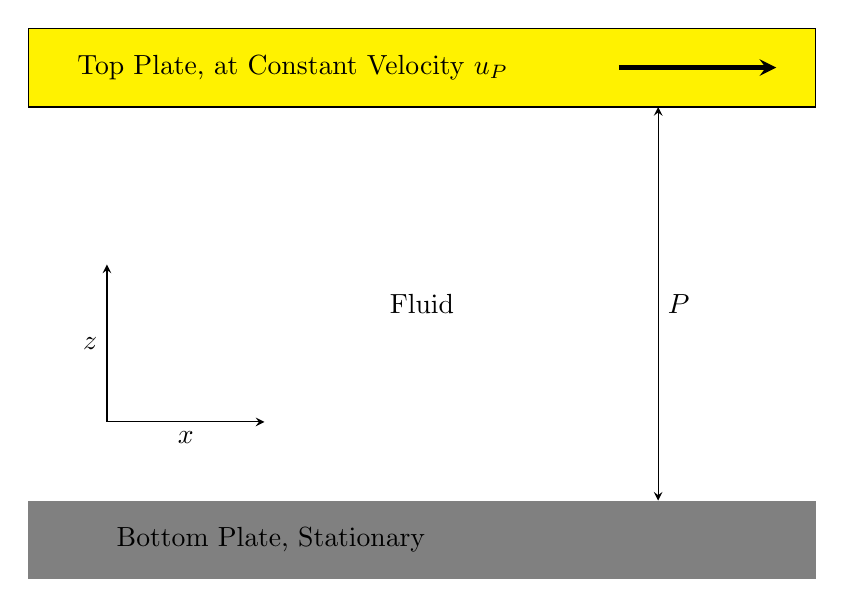
\begin{tikzpicture}    [> = stealth]

\filldraw[fill=yellow, draw=black] (0,5) rectangle (10,6);
\fill[color=gray] (0,0) rectangle (10,-1);

\node at (0.5,5.5) [right] {Top Plate, at Constant Velocity $u_{P}$};
\node at (5,2.5) {Fluid};
\node at (1,-0.5) [right] {Bottom Plate, Stationary};

\draw [->, ultra thick] (7.5,5.5) -- +(2,0);

\draw [<->] (1,3) -- node[left] {$z$} ++(0,-2) -- node[below] {$x$} +(2,0);

\draw [<->] (8,0) -- node[right] {$P$} +(0,5); 

\end{tikzpicture}
\caption{The system of Couette flow} \label{Couettesystem}
\end{figure}

This setup is amenable to experimental measurement; the point of theoretical physics is to generate a prediction of the measurements using mathematical reasoning.  To that end, we need a mathematical model of the physical situation.
We work in $\mathbb{R}^{3}$, with $z$ being the vertical direction, and $x$ the left-to-right horizontal direction. The fluid is modeled as a \emph{continuum} velocity field $\vec{u}(x,y,z) = (u,v,w) $ obeying the Navier-Stokes equations at all points. The boundaries of the fluid -- the two plates -- are modeled as perfect $x,y$ planes, separated by a width $P$. The bottom boundary is the plane $z=0$, the top the plane $z=P$.
The bottom boundary is stationary, while the top boundary has a constant velocity $\vec{u}_P$ in the $x$ direction (with magnitude $u_{P}$). 

To solve the Navier-Stokes equations, a boundary condition is required. Let's start with the simple classical case of no slip. Since the fluid sticks to the boundaries, the fluid at the bottom boundary has zero velocity, while fluid at the top boundary has velocity $\vec{u}_{P}$. 
The fluid has \emph{viscosity}, that is, a layer of fluid atoms sliding over another layer causes a shear stress that tends to accelerate the lower layer.  By this mechanism, the driving plate drives the entire bulk fluid, as the driving velocity propagates down through the fluid.
%The fluid is driven by the driving plate, and viscosity causes shear stress, accelerating %fluid in the bulk. 
The steady-state solution is that the fluid velocity is in the $x$ direction only, with a magnitude $u(z)$ that changes linearly between 0 at the bottom and $u_{P}$ at the top:

\begin{equation}
u(z) = \frac{z}{P}u_{P}  
\end{equation}

A schematic of Couette flow with its characteristic linear velocity gradient appears in Figure (\ref{Couetteflow}).

\begin{figure}[ht]
\centering
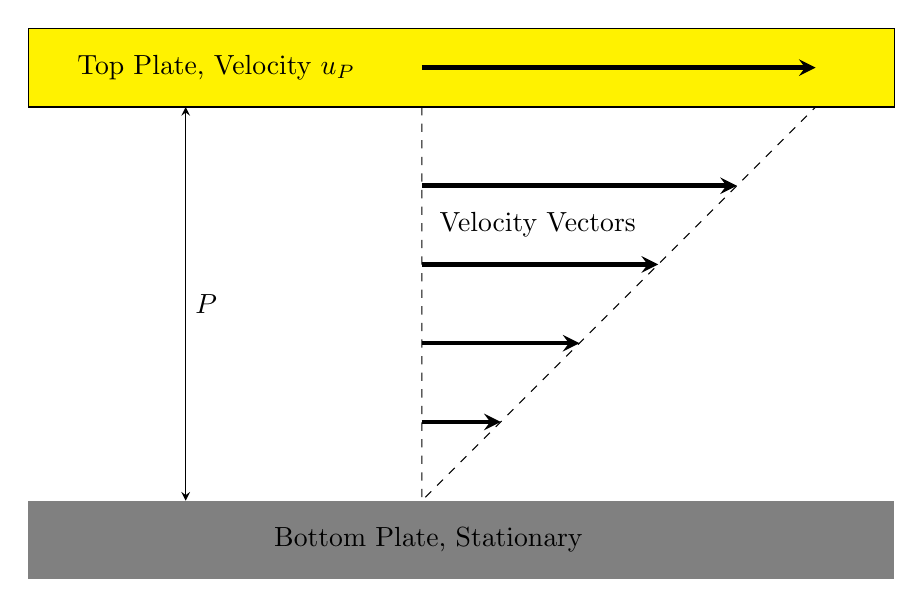
\begin{tikzpicture}    [> = stealth]

\filldraw[fill=yellow, draw=black] (-1,5) rectangle ++(11,1);
\fill[color=gray] (-1,0) rectangle (10,-1);

\node at (-0.5,5.5) [right] {Top Plate, Velocity $u_{P}$};
\node at (4.1,3.5) [right] {Velocity Vectors};
\node at (2,-0.5) [right] {Bottom Plate, Stationary};

\draw [->, ultra thick] (4,5.5) -- +(5,0);

\draw [<->] (1,0) -- node[right] {$P$} +(0,5); 

% x,z axes
%\draw [<->] (1,3) -- node[left] {$z$} ++(0,-2) -- node[below] {$x$} +(2,0); 

\foreach \z in {1,2,3,4}
  \draw [->, ultra thick] (4,\z) -- +(\z,0);

\draw [dashed] (4,5) -- +(0,-5) -- +(5,0);  

\end{tikzpicture}
\caption{Couette flow} \label{Couetteflow}
\end{figure}

Now let's relax the no slip condition and consider some kind of \emph{slip} boundary condition. The simplest such condition is that there is a finite slip velocity at the surface, and that velocity is proportional to the \emph{shear rate} in the fluid. This condition was first proposed by Navier:

\begin{equation}
u_{\mathrm{slip}} = b \frac{\partial u}{\partial z}
\end{equation}

The constant of proportionality $b$, has units of length, and accordingly is known as the \emph{slip length.}

Since the shear stress is proportional to the shear rate, the Navier slip relation says that the shear stress on the fluid at the boundary is proportional to the fluid velocity at the boundary.

In the model in use here, the slip length has a simple geometric interpretation: 
The velocity gradient at the wall may be linearly extrapolated \emph{into} the wall. The distance into the wall at which the velocity \emph{would} be zero, is the slip length.

Couette flow with a non-zero slip length is shown in Figure (\ref{Couetteslip}).

\begin{figure}[ht]
\centering
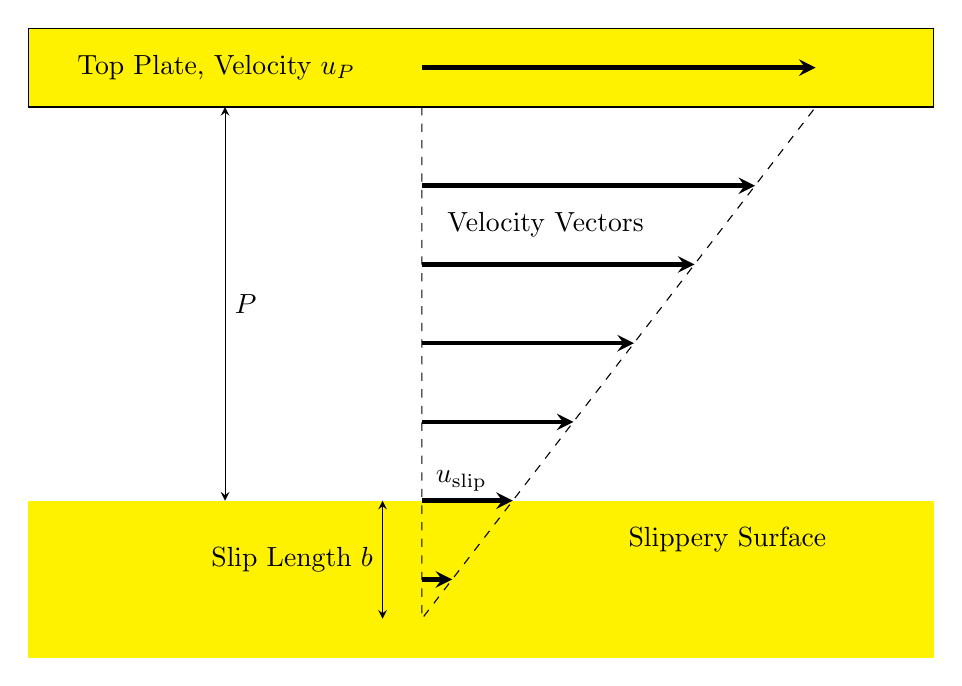
\begin{tikzpicture}    [> = stealth]

\filldraw[fill=yellow, draw=black] (-1.5,5) rectangle ++(11.5,1);
\fill[color=yellow] (-1.5,0) rectangle ++(11.5,-2);

\node at (-1,5.5) [right] {Top Plate, Velocity $u_{P}$};
\node at (3.7,3.5) [right] {Velocity Vectors};
\node at (6,-0.5) [right] {Slippery Surface};

\draw [->, ultra thick] (3.5,5.5) -- +(5,0);

\draw [<->] (1,0) -- node[right] {$P$} +(0,5); 

% x,z axes
%\draw [<->] (1,3) -- node[left] {$z$} ++(0,-2) -- node[below] {$x$} +(2,0); 

\foreach \z in {-1,0,1,2,3,4}
  \draw [->, ultra thick] (3.5,\z) -- +(\z*0.76923 + 1.1545 ,0);

\draw [dashed] (3.5,5) -- +(0,-6.5) -- +(5,0); 

\draw [<->] (3,0) -- node[left] {Slip Length $b$} +(0,-1.5); 

\node at (4,0)[above] {$u_{\mathrm{slip}}$};

\end{tikzpicture}
\caption{Couette flow with slip} \label{Couetteslip}
\end{figure}

At this point we stop to emphasize that the slip length is a feature of the \emph{mathematical model.} We have assumed two things: First, the boundary between fluid and solid is a perfect Euclidean plane. Second, the fluid is a continuum, allowing for a well-defined velocity gradient at the boundary. Reconciling this Platonic ideal with a real physical experiment is non-trivial. We shall go into some depth with this issue shortly.

The slip length is a property of the fluid/solid interface, and can in principle vary in space. This leads us to the concept of \emph{effective slip length}, the calculation of which is the subject of this thesis.

%\clearpage
\section{Effective Slip Length}

Working again with the same model, let us assume the slip length $b$ is a parameter that varies over the solid surface. 
This could model the case when the surface \emph{material} changes spatially, eg.\ high-slip Teflon regions on a no-slip metal surface.
Again, we seek a velocity flow field description of the fluid. In this case, a simple solution is not readily apparent --- the problem has essentially gained an extra dimension. In fact, there are no known analytical solutions to this general problem.

The flow field near the surface will no longer be a straightforward laminar flow, but will be perturbed by the spatial variations in slip length. However, we would expect those perturbations to decay with increasing height above the surface. At sufficient height, the perturbations will be essentially zero, and the flow will be uniform laminar flow. This uniform flow has a shear rate that does not vary over space.  Therefore, the velocity gradient can be extrapolated down to the solid surface, and \emph{into} the surface, defining an \emph{effective} slip length.

This is illustrated in Figure (\ref{effslip}).

\begin{figure}[ht!]
\centering
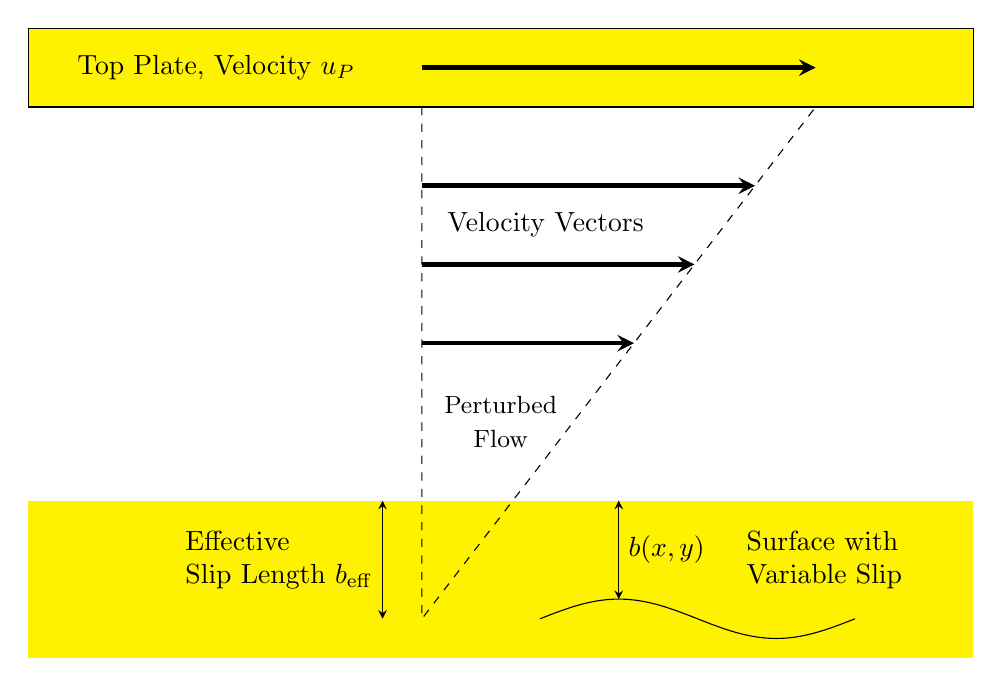
\begin{tikzpicture}    [> = stealth]
\renewcommand{\baselinestretch}{1.00}

\filldraw[fill=yellow, draw=black] (-1.5,5) rectangle ++(12,1);
\node at (-1,5.5) [right] {Top Plate, Velocity $u_{P}$};
\draw [->, ultra thick] (3.5,5.5) -- +(5,0);
 
\fill[color=yellow] (-1.5,0) rectangle ++(12,-2); 
 
\foreach \z in {2,3,4}
  \draw [->, ultra thick] (3.5,\z) -- +(\z*0.76923 + 1.1545 ,0);
\draw [dashed] (3.5,5) -- +(0,-6.5) -- +(5,0); 
\node at (3.7,3.5) [right] {Velocity Vectors};

\node at (4.5,1) [align=center] {\small Perturbed\\ \small Flow};

\node at (7.5,-0.75) [right,align=left] {Surface with\\ Variable Slip};

\draw [<->] (3,0) -- node[left, align=left] {Effective\\Slip Length $b_{\mathrm{eff}}$} +(0,-1.5); 

\draw (5,-1.5) sin ++(1,0.25) cos ++ (1,-0.25) sin ++(1,-0.25) cos ++(1,0.25);
\draw[<->] (6,0) -- node[right] {$b(x,y)$} ++(0,-1.25);

\end{tikzpicture}
\caption{Effective slip length} \label{effslip} 
\end{figure}


\vspace{1em}
The far-field flow of the system is equal to that of an \emph{effective} system, defined as follows:  The effective system has the same top boundary condition, but has a no-slip boundary condition holding on a lower surface located distance $\beff$ below the surface of the original system.

The no-slip plane of the effective system is denoted the \textbf{effective no-slip plane.}
Hence, the effective slip length of the system of perturbed Couette flow is the distance that the effective no-slip plane lies below the physical surface plane.  See Figure (\ref{effnoslip}).


\begin{figure}[ht!]
\centering
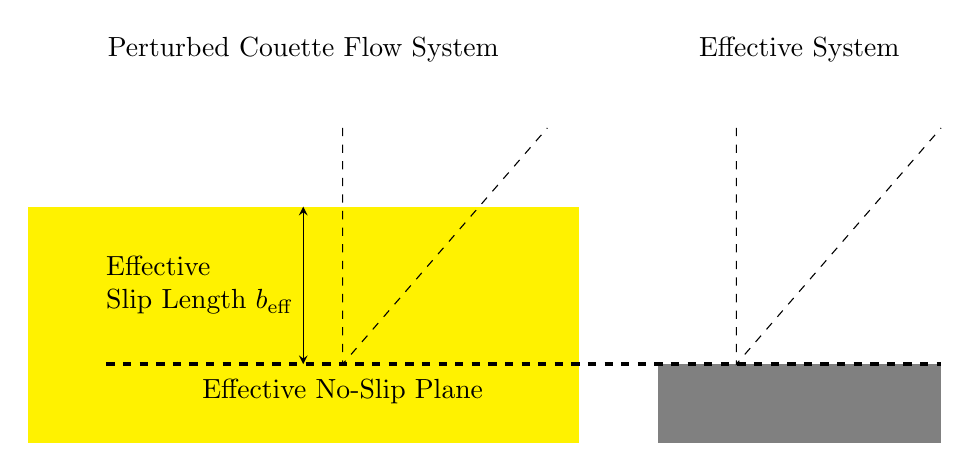
\begin{tikzpicture}  [> = stealth]
\renewcommand{\baselinestretch}{1.00}

\fill[color=yellow] (0,0) rectangle (7,-3);

\draw [<->] (3.5,0) -- node[left, align=left] {Effective\\Slip Length $b_{\mathrm{eff}}$} ++(0,-2);
\draw[dashed] (4,1) -- ++(0,-3) -- ++(2.6,3);

\fill[color=gray] (8,-2) rectangle ++(3.6,-1);
\draw[dashed] (9,1) -- ++(0,-3) -- ++(2.6,3);

\draw[very thick, dashed] (1,-2) -- ++(10.6,0);
\node at (4,-2.35) {Effective No-Slip Plane};

\node at (3.5,2) {Perturbed Couette Flow System};
\node at (9.8,2) {Effective System};
\end{tikzpicture}
\caption{Effective no-slip plane} \label{effnoslip} 
\end{figure}


\clearpage

\section{Effective Slip Length of Rough Surface}

We now extend the model, allowing the solid surface to be \emph{rough} rather than just flat. 
%The surface is now \emph{rough}, perhaps corrugated. 
We allow the local slip length to vary over the surface, as before.

%The definition of effective slip is the same as before, but with an important extension: The position of the solid/liquid interface is now a \emph{range.} Therefore, the effective slip length can be defined with respect to any position in that range. We let the surface be a function $h(x,y)$, (nominally centered at $z=0$), bounded by $h_{\mathrm{min}}$ and $h_{\mathrm{max}}$. Define $\Delta h = h_{\mathrm{max}} - h_{\mathrm{min}}$. Then plausible definitions of $\beff$ lie in the range $[b_{0}, b_{0} + \Delta h]$, where $b_{0}$ is the minimum \emph{effective} slip length --- not the minimum \emph{local} slip length.

The definition of effective slip now acquires a subtlety: the solid-liquid interface is no longer a flat plane.  The system still behaves like an effective system with an effective no-slip plane located below the physical surface.  But now the distance from the physical surface to the effective no-slip plane is ambiguous. In principle, one could measure the distance from the troughs of the rough surface, or the peaks, or any point in between. 
See Figure (\ref{effsliprough}). In fact, as we shall see in Chapter 3, this ambiguity caused apparent contradictions in the measurement of effective slip on rough surfaces, as different researchers adopted different conventions.



\begin{figure}[ht]
\centering
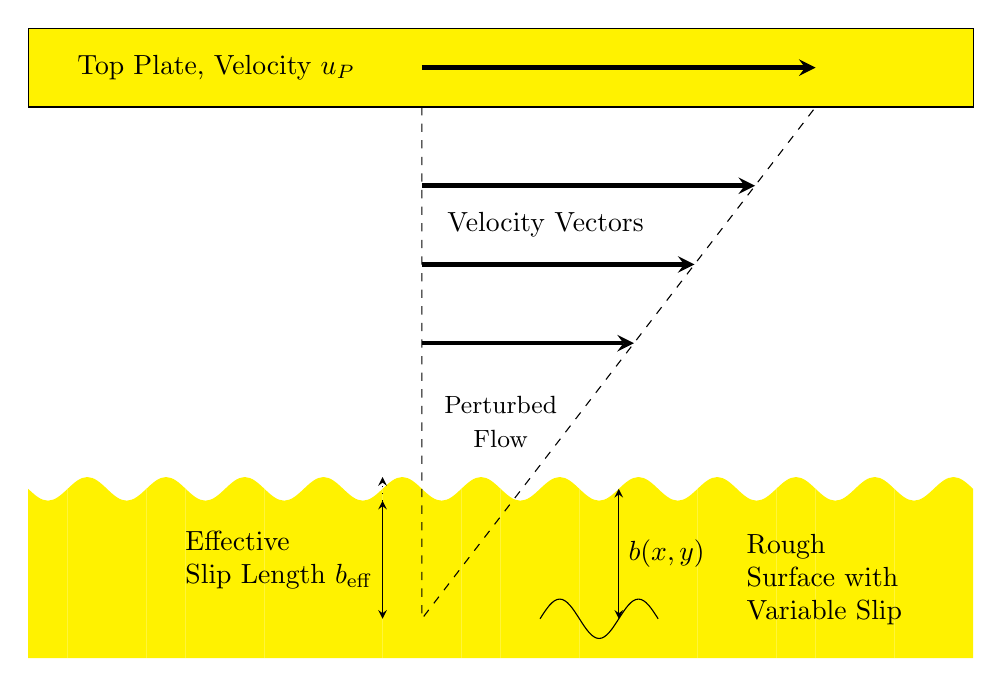
\begin{tikzpicture}    [> = stealth]
\renewcommand{\baselinestretch}{1.00}

\filldraw[fill=yellow, draw=black] (-1.5,5) rectangle ++(12,1);
\node at (-1,5.5) [right] {Top Plate, Velocity $u_{P}$};
\draw [->, ultra thick] (3.5,5.5) -- +(5,0);

%\fill[color=yellow] (-1.5,0) rectangle ++(12,-2);
\foreach \x in {-1,...,10}
               {   \fill[color=yellow] (\x,-2) -- ++(0,2.15) sin ++(0.25,0.15)
                   cos ++(0.25,-0.15) |- ++(-0.5,-2.15);   }
\foreach \x in{-2,...,9} 
              {   \fill[color=yellow] (\x+ 0.5,-2) -- ++(0,2.15) sin ++(0.25,-0.15)
                  cos ++(0.25,0.15) |- ++(-0.5,-2.15);    }

\foreach \z in {2,3,4}
  \draw [->, ultra thick] (3.5,\z) -- +(\z*0.76923 + 1.1545 ,0);
\draw [dashed] (3.5,5) -- +(0,-6.5) -- +(5,0); 
\node at (3.7,3.5) [right] {Velocity Vectors};

\node at (4.5,1) [align=center] {\small Perturbed\\ \small Flow};

\node at (7.5,-1) [right,align=left] {Rough\\Surface with\\ Variable Slip};

\draw [<->] (3,0) -- node[left, align=left] {Effective\\Slip Length $b_{\mathrm{eff}}$} +(0,-1.5); 
\draw [dotted, ->] (3,0) -- +(0,0.3);

\draw (5,-1.5) sin ++(0.25,0.25) cos ++(0.25,-0.25) sin ++(0.25,-0.25)
               cos ++(0.25,0.25) sin ++(0.25,0.25) cos ++(0.25,-0.25);
\draw[<->] (6,0.15) -- node[right] {$b(x,y)$} ++(0,-1.65);

\end{tikzpicture}
\caption{Effective slip length of rough surface} \label{effsliprough} 
\end{figure}

\clearpage

Defining a nominal surface plane at the \textbf{tops of the peaks} of the surface roughness is a defensible choice.  See Figure (\ref{rougheffnoslip}). That way, pure bulk conditions hold above the nominal surface.
Furthermore, physical instruments probing the position of the surface would tend to encounter the tops of the peaks, and record this as the surface position.
Incidentally, this convention has the effect of maximizing effective slip lengths measured on rough surfaces.  


\begin{figure}[ht!]
\centering
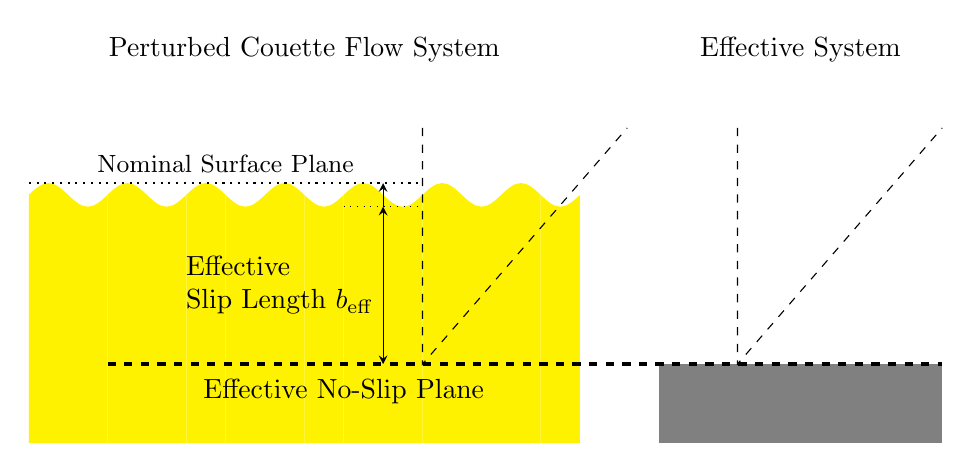
\begin{tikzpicture}  [> = stealth]
\renewcommand{\baselinestretch}{1.00}

%\fill[color=yellow] (0,0) rectangle (7,-3);

\foreach \x in {0,...,6}
               {   \fill[color=yellow] (\x,-3) -- ++(0,3.15) sin ++(0.25,0.15)
                   cos ++(0.25,-0.15) |- ++(-0.5,-3.15);   }
\foreach \x in{0,...,6} 
              {   \fill[color=yellow] (\x+ 0.5,-3) -- ++(0,3.15) sin ++(0.25,-0.15)
                  cos ++(0.25,0.15) |- ++(-0.5,-3.15);    }


\draw[dotted] (4,0) -- ++(1,0);
\draw[thick, dotted] (0,0.3) -- node[above]{\small Nominal Surface Plane} ++(5,0);

\draw [<->] (4.5,0) -- node[left, align=left] {Effective\\Slip Length $b_{\mathrm{eff}}$} ++(0,-2);
\draw [->] (4.5,0) -- ++(0,0.3);

\draw[dashed] (5,1) -- ++(0,-3) -- ++(2.6,3);

\fill[color=gray] (8,-2) rectangle ++(3.6,-1);
\draw[dashed] (9,1) -- ++(0,-3) -- ++(2.6,3);

\draw[very thick, dashed] (1,-2) -- ++(10.6,0);
\node at (4,-2.35) {Effective No-Slip Plane};

\node at (3.5,2) {Perturbed Couette Flow System};
\node at (9.8,2) {Effective System};
\end{tikzpicture}
\caption{Effective no-slip plane with rough surface} \label{rougheffnoslip} 
\end{figure}

\clearpage

\section{Purpose of Thesis}

The purpose of this thesis is to present a theory with which to predict the effective slip length, given knowledge of the local slip length:

\begin{equation}
b_{\mathrm{eff}} = f(b(x,y))
\end{equation}

Furthermore, the theory can deal with a rough surface, where the rough surface is described by a height function $h(x,y)$:
%Second, to extend the theory, taking into account the rough surface.

\begin{equation}
\beff = f(b(x,y),h(x,y))
\end{equation}

We present a formula for $\beff$, in the idealized case where surface roughness is periodic, and the local slip length varies with the same period, in the limiting case where the local slip length is always large compared to the period of surface roughness.

The answer turns out to be that $\beff$ is the area-weighted \emph{harmonic} average of the local slip length, where the area in question is the area of contact between solid and liquid.


\begin{equation}
\beff = \left< \frac{\sqrt{1+h'^{2}}}{b}  \right > ^{-1}
\end{equation}

The core of this thesis is a rigorous derivation of this result.

\vspace*{1em}
We also confirm, using a completely different mathematical technique, the special case of a flat surface:
\begin{equation}
\beff = \left< \frac{1}{b}  \right > ^{-1}
\end{equation}
We further show that for a flat surface, in the opposite limiting case where the period is large compared to any local slip length, that $\beff$ is the area-weighted average of local slip lengths:
\begin{equation}
\beff = \left< b  \right >
\end{equation}


\section{Application of Thesis}

%The question of whether or not fluid slips at the solid boundary is fundamental to fluid mechanics, in the sense that a %solution to the Navier Stokes equations requires a boundary condition, and the no-slip boundary condition was accepted by %consensus only after lengthy controversy.

The question of whether or not fluid slips at the solid boundary is fundamental to fluid mechanics in the following sense: To solve the Navier Stokes equation, a boundary condition is needed, and the no-slip condition was accepted by consensus only after lengthy controversy.
However, in almost all practical applications, plumbing, drainage, ship building etc., it turns out that any slip will be too small to matter.  At the macro scale, the no-slip boundary condition is observed.

Only recently has the possibility of fluid slip become important, in the new fields of microfluidics and nanofluidics.  In these fields, researchers and engineers fabricate devices in which fluid flows through pipes with a width measured in microns, or even smaller.  In such channels, the high surface area to volume ratio works strongly against fluid flow.  If the no-slip condition could be relaxed, then flow rates could be increased significantly.

Hydrophobic channel walls give the possibility of a non-zero intrinsic slip length.  However, larger slip effects are attempted by creating surfaces that contain regions of \emph{air,} perhaps trapped in small pockets on the surface.  Then the fluid flows partly over an air-water interface, which is expected to have a large intrinsic slip length. Experiments show increased flow rates through channels with such walls \cite{OuPerotRothstein2004, HyvaluomaHarting2008}.

The question is then \emph{how much} would flow rates increase with these exotic surfaces.  This can be rephrased as `what is the effective slip length of the surface?'  This thesis offers a means of calculating the effective slip length for some cases.

\clearpage

\section{Structure of Thesis}

The core of this thesis is essentially the shortest possible physically and mathematically rigorous derivation of the harmonic mean formula for $\beff$.  The remainder of the thesis consists of an alternative derivation of a special case of the harmonic mean formula, a derivation of another formula for $\beff$ in the complementary regime, some numerical testing, and a brief look at some analogues of effective slip in other physical systems.

Chapter 2 `Does Slip Exist?' reviews the literature on slip, focussing at reasonable depth on the (few) papers that credibly demonstrate intrinsic slip on a clean, atomically flat surface.  It ultimately concludes that an intrinsic slip length of 10 - 20 nm has been seen on hydrophobic surfaces.

Chapter 3 `Mixed Slip Flow' looks at flow over surfaces that are rough, or have a varying intrinsic slip length.  The focus is on `superhydrophobic' surfaces and nanobubbles, and the importance of carefully locating the $z=0$ plane.

Chapter 4 `Effective Slip Length Expressions: Prior Work' is a literature review of previous results for an effective slip length.  Since the work in this thesis has been published as three papers \cite{HendyLund2007, LundHendy2008, Lund2012}, the work is easily placed in context with other peer-reviewed articles.

Chapter 5 `The Mathematical Model' sets up the formal mathematical framework, including the definition and explanation of the velocity gradient tensor, and the simplification to Stokes flow.

Chapter 6 `The Homogenized Effective Slip Length' is the core of the thesis: The technique for solving partial differential equations known as homogenization is explained in some detail, and then applied to the effective slip problem.  An expression for $\beff$ is derived for the regime where the period is much smaller than any local slip length.

Chapter 7 `Perturbative Effective Slip Lengths' uses the completely different technique of perturbation methods to derive $\beff$ for the special case of a flat surface.  Also derived is another expression for $\beff$ that applies in the contrasting regime where the period is much larger than slip lengths.

Chapter 8 `Numerics' shows that numerical simulations using finite element modelling are in excellent agreement with our expression for $\beff$.

Chapter 9 `Analogues of Effective Slip' takes a brief look at other physical problems that happen to be described by a very similar mathematical model to that analysed in Chapter 5, and therefore have a similar solution.  A problem in thermal insulation, and a problem in catalysis are given a brief treatment.

Chapter 10 `Conclusion' summarises and considers future extensions to the work.


\section{Publications from the Work of this Thesis}

The work of the this thesis has been published as three papers, with the second subsuming the first.  The first was written by my supervisor Dr Shaun Hendy, describing the use of a perturbation method to derive effective slip lengths for a one-dimensional flat surface \cite{HendyLund2007}.  I then extended the perturbation method to derive effective slip lengths for 3-D flow over a two-dimensional flat surface.  This work generalised the earlier result, and I wrote a paper describing it in 2008 \cite{LundHendy2008}.  I then used the homogenization method to derive an effective slip length for rough surfaces.  I wrote a paper describing this in 2012 \cite{Lund2012}.

\iftoggle{compilealone}
    {
    \bibliography{Lund_Thesis.bib}
    \bibliographystyle{plain}
    }

\end{document}

% Finished August 17, 2012
% Split in half October 15, 2013.  (This is the second half.)
% Put into VUW thesis format (with Figure numbers) November 2013.

\documentclass[12pt, a4paper, twoside, openright]{book}

\usepackage{vuwthesis} % sets up some local things, mostly the front page

\setlength{\intextsep}{12pt} % set space above and below in-line float
\setlength{\abovecaptionskip}{0pt} % set space between figure and caption.


\usepackage{amssymb, amsmath}
\usepackage{tikz}

\newcommand{\beff}{\ensuremath{b_{\mathrm{eff}}}}
\newcommand{\ewf}{\ensuremath{\epsilon_{\mathrm{wf}}}}
\newcommand{\vslip}{\ensuremath{v_{\mathrm{slip}}}}

\newcommand{\paper}[1]
         {\colorbox[gray]{0.8}{ \textsc{#1}}
         
         }
         
\usepackage{etoolbox}
\newtoggle{compilealone}
\toggletrue{compilealone}

\author{Nat Lund}
\title{Chapter 2: Does Slip Exist?}

\begin{document}
\chapter{Does Slip Exist?}\label{C:slip}


A theory of effective slip could be treated as a purely mathematical result, with the slip length being simply a parameter in the model.  However, a theory of effective slip has practical value only if the slip length parameter has some physical meaning: quantifying the slip effect for flow over a homogeneous physical surface.  Establishing that a slip effect exists on clean, atomically flat surfaces is far from trivial.  Therefore, in this chapter we will examine the literature on the experimental and theoretical evidence for slip.

This cannot be a comprehensive review of all available literature, but rather will be a sample of some high-profile papers.
An exhaustive review of the experimental literature is available in the 2005 review article by Neto \emph{et al} \cite{NetoReview2005}. Other comprehensive reviews are by Vinogradova in 1999 \cite{VinogradovaReview1999} and Lauga, Brenner and Stone in 2006 \cite{LaugaReview2006}. A reasonable introduction is the progress article of Granick \emph{et al} from 2003 \cite{GranickReview2003}.

\section{Types of Slip}

So far, we have discussed slip within a mathematical model of fluid flow; this is deliberate: in such a model the concepts of slip and slip length are straightforward and intuitive. However, we now need to tackle slip in the real world, disentangling a partially-ordered hierarchy of concepts.

\clearpage
\subsection{Definitions in the Literature}

The 2006 review article by Lauga, Brenner and Stone \cite{LaugaReview2006} proposes the following definitions (some paraphrased):

\begin{itemize}

\item \textbf{Phenomenon of slip:} A fluid dynamics system behaving as if the fluid velocity at the wall differs from the wall velocity.

\item \textbf{Molecular slip} (also intrinsic slip): `Refers to the possibility of using hydrodynamics to force liquid molecules to slip against solid molecules.'

\item \textbf{Apparent slip:} The case when the no-slip condition holds on the surface, but at larger length scales, the no-slip condition appears not to be valid.

\item \textbf{Effective slip:} `Refers to the case where molecular or apparent slip is estimated by averaging an appropriate measurement over the length scale of an experimental apparatus.'

\end{itemize}


These definitions are a good place to start.  But they make no mention of \emph{mixed-slip} surfaces.  We shall accept these definitions, but modify and extend them to deal cleanly with the separate cases of pure \emph{and} mixed-slip surfaces.

The first modification is to separate molecular slip from intrinsic slip.

\begin{itemize}
\item \textbf{Intrinsic Slip:} When a clean, atomically flat homogeneous surface behaves as if the no-slip condition does not hold.
\end{itemize}

With this definition, Intrinsic Slip may be due to Molecular Slip or Apparent Slip.

The second modification is to take Lauga \emph{et al}'s concept of `Effective Slip' and simplify it, then relabel it as simply `Measured Slip'.

\begin{itemize}
\item \textbf{Measured Slip:} A slip effect measured with some experimental apparatus.
\end{itemize}

This allows us to use the phrase `Effective Slip' to emphasize the possible heterogeneity of the surface:

\begin{itemize}
\item \textbf{Effective Slip:} A slip effect imputed to liquid-solid interface, where the surface is not known to be homogeneous and atomically flat.
\end{itemize} 

We shall discuss some of these concepts in more depth.

\subsection{Measured Slip}
As we shall see shortly, all measurements are to some extent indirect: Experiments cannot yet directly probe the fluid velocity in the region within a few nanometers of the surface. A measurement of a slip effect may be measuring molecular slip, apparent slip, or, for a heterogeneous surface, any combination of the two.

There are no direct measurements of slip; if there were, they would be measuring molecular slip.


\subsection{Intrinsic Slip}
%Next, we turn our attention to the \emph{material} of the surface exhibiting  slip effect. 
Suppose we can prepare a perfectly clean, atomically flat sample of some material. Further, suppose we can experimentally test the sample for slip effects with some pure liquid.
% (pure water, say). 
If a slip effect appears, and can be consistently replicated, then the implied slip length is a meaningful, reliable parameter of the fluid-solid system. It is reasonable to label this the \emph{intrinsic} slip length.

Intrinsic slip may be due to molecular slip or apparent slip.


\subsection{Molecular Slip}
`True slip' means that the fluid \emph{at the boundary} has a non-zero velocity.
At the smallest scale, the fluid velocity at a point is the average velocity of an ensemble of molecules.  Thus, `true' slip means that the average velocity of the molecules in contact with the wall is non-zero.
This implies that the molecules in contact with the wall are \emph{not} all sticking to the wall all the time.
If (some) fluid molecules at the surface are slipping along the surface, this is termed molecular slip.

There are no direct observations of molecular slip, though (as explained later) it is observed in molecular dynamics computer simulations.

A hypothetical mechanism for molecular slip in liquids could be one similar to the (known) mechanism for slip in gases -- Knudsen Slip:


\subsubsection{Molecular Slip in Gases -- Knudsen Slip}
%% Rewriting, 8 Jan 2014:
In a gas, the mean free path is many times larger than the gas molecule size, so an interaction with the wall will almost certainly not involve another gas particle.  Therefore, the interaction can be treated as a simple reflection.

A gas particle has some momentum in the direction tangent to the wall.  If an incident gas particle simply \emph{sticks} to the wall, then all of its tangential momentum is transferred to the wall.  This is the case of `stick' or the no-slip condition.  If the particle subsequently detaches with a velocity in a random direction, \emph{on average} its tangential momentum will still be zero -- the same as the wall.

At the other extreme, suppose that an incident particle undergoes specular reflection, bouncing off the wall with no change in its tangential momentum.  With no momentum loss, there is no `friction', and the gas experiences perfect slip.
% This is Knudsen slip.

While specular reflection is defined as the equality of well-defined angles of incidence and reflection, the key aspect of the interaction is that the wall-particle force is always perpendicular to the wall, so the wall cannot change the tangential momentum of the colliding particle.
This will always be the case if the wall is perfectly flat and rigid,
although this is an idealised limiting case.
In real systems exhibiting Knudsen slip, only some fraction of gas particles will undergo specular or close-to-specular reflection. 

An effect similar to Knudsen slip may occur in fluids, although the mean free path in a liquid is generally less than the molecular diameter, so angles of incidence and reflection become difficult to define.  However, particle-wall collisions in which the particle loses no tangential momentum may still occur.  A computer simulation where the wall is defined as perfectly flat and rigid would allow this.


\subsection{Apparent Slip}

%While slip effects are generally acknowledged, the existence of molecular slip remains debatable. 
Perhaps the simplest alternative to molecular slip to explain slip effects is apparent slip. The idea is that there exists a \emph{boundary layer} of reduced viscosity at the solid surface. As a consequence of the lower viscosity, the velocity gradient in the boundary layer is \emph{steeper} than in the bulk. Thus, the velocity gradient `turns a corner' at the interface between boundary layer and bulk. The no-slip condition holds at the solid-liquid interface, but the velocity gradient in the bulk can be extrapolated to generate a slip length, as shown in Figure (\ref{depletion}).

\begin{figure}[ht]
\centering
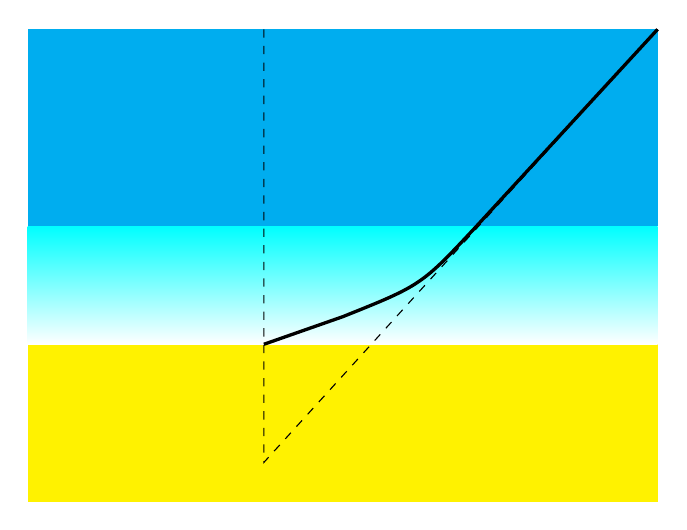
\begin{tikzpicture}

\fill[color=yellow] (-3,-2) rectangle (5,0);

\fill[color=cyan] (-3,1.5) rectangle (5,4);
\shade [top color=cyan] (-3,0) rectangle (5,1.5);

\draw[dashed] (0,4) -- (0,-1.5) -- (5,4);

\draw[very thick] (0,0)--(1.0,0.35) .. controls (2, 0.75) .. (2.7,1.5)--(5,4);

\end{tikzpicture}
\caption{Apparent slip caused by a depletion layer with lower-than-bulk viscosity.} \label{depletion}
\end{figure}

%The boundary is very thin compared to experimental length scales. The reduction in viscosity is commensurate with a reduction in density; indeed, de Gennes notes that observed slip effects are explainable by a \emph{gas} layer, only 1 or 2 atoms thick \cite{deGennes2002}.

%Only a very thin low-density layer is required to explain observable effects:
%de Gennes notes that observed slip effects are explainable by a \emph{gas} layer, only 1 or 2 atoms thick \cite{deGennes2002}.

If the boundary layer has sufficiently low density, then only a very thin layer is required to explain observed effects:  de Gennes notes that observed slip effects are explainable by a \emph{gas} layer, only 1 or 2 atoms thick \cite{deGennes2002}.


\clearpage

\subsection{Types of Slip Redux}

We summarize the hierarchy of slip concepts in Figure (\ref{slipconcepts}) below:

\begin{figure}[ht]
\centering
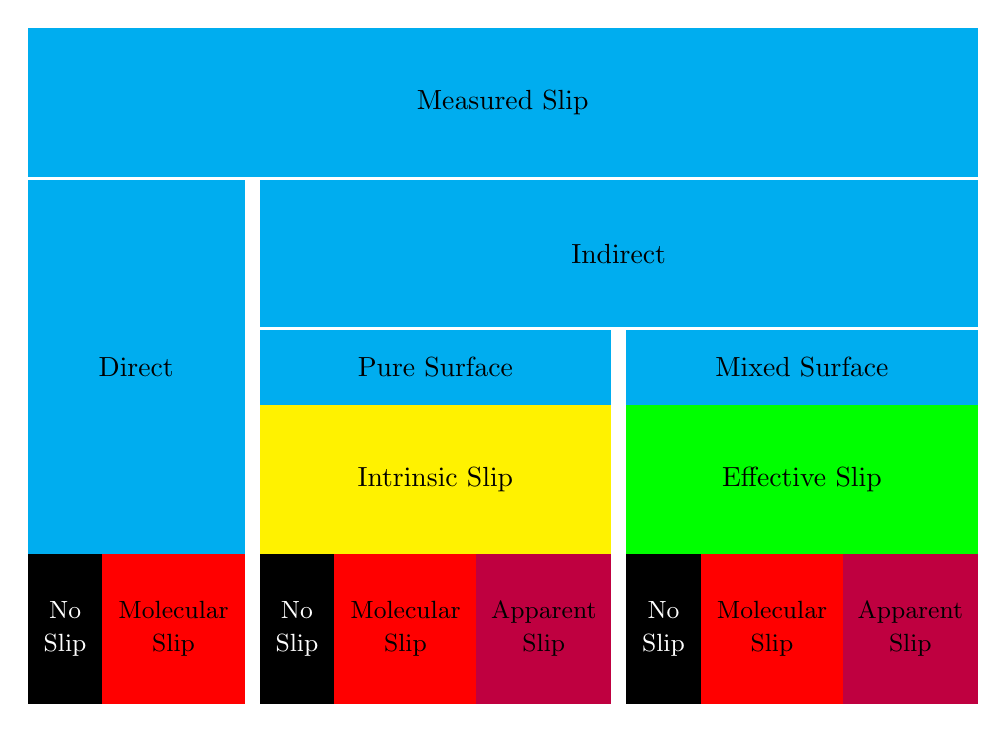
\begin{tikzpicture} [scale=0.95]
\renewcommand{\baselinestretch}{1.00}
% Depending on some random factors, the rectangles may appear on screen to have faint white
% borders between them, or not.  The slight separation is good.  So I have made this explicit
% by lifting the bottom of Measured Slip and Indirect rectangles by 0.04 cm 

\fill[color=black] (0,0) rectangle node[color=white,align=center] 
{\small No\\ \small Slip} +(1,-2);
\fill[color=red] (1,0) rectangle node[color=black,align=center] 
{\small Molecular\\ \small Slip} +(1.9,-2);

\fill[color=black] (3.1,0) rectangle node[color=white,align=center] 
{\small No\\ \small Slip} +(1,-2);
\fill[color=red] (4.1,0) rectangle node[color=black,align=center] 
{\small Molecular\\ \small Slip} +(1.9,-2);
\fill[color=purple] (6,0) rectangle node[color=black,align=center]
{\small Apparent\\ \small Slip} +(1.8,-2);

\fill[color=black] (8,0) rectangle node[color=white,align=center] 
{\small No\\ \small Slip} +(1,-2);
\fill[color=red] (9,0) rectangle node[color=black,align=center] 
{\small Molecular\\ \small Slip} +(1.9,-2);
\fill[color=purple] (10.9,0) rectangle node[color=black,align=center]
{\small Apparent\\ \small Slip} +(1.8,-2);

\fill[color=cyan] (0,0) rectangle node[color=black] {Direct} +(2.9,5);
\fill[color=cyan] (0,5.04) rectangle node[color=black] {Measured Slip} +(12.7,2);

\fill[color=yellow] (3.1,0) rectangle node[color=black] {Intrinsic Slip} +(4.7,2);
\fill[color=cyan] (3.1,2) rectangle node[color=black] {Pure Surface} +(4.7,1);

\fill[color=green] (8,0) rectangle node[color=black] {Effective Slip} +(4.7,2);
\fill[color=cyan] (8,2) rectangle node[color=black] {Mixed Surface} +(4.7,1);

\fill[color=cyan] (3.1,3.04) rectangle node[color=black] {Indirect} +(9.6,1.96);

\end{tikzpicture}
\caption{Hierarchy of slip concepts.} \label{slipconcepts}
\end{figure}

Note that the `Direct Measurement' category is there just for completeness -- as mentioned,  experiments cannot presently verify molecular slip.

\clearpage
\section{Experimental Intrinsic Slip}

Probably the first credible experiments showing a slip effect are those by Erhard Schnell in 1956 \cite{Schnell1956}. In a series of careful experiments, Schnell treated glass capillaries with dimethyldichlorosilane to make them hydrophobic. The silicone layer decreased the capillary diameter by 0.01\% to 0.04\%. Nevertheless, at sub-turbulent velocities, the hydrophobic capillaries flowed 0\% - 5\% more water than otherwise-identical untreated capillaries. He attributed this excess flow to slip: `` ...this can only be explained by the slippage of water over the non-wettable surface."  
%Note that Schnell did not mention `slip length'.

After Schnell, various experiments that illustrated slip were reported. But, it is fair to say that it wasn't until the 21st century that truly believable evidence appeared.
Modern experimental techniques on slip progressed rapidly, starting from the 1990s, particularly the after widespread availability of the Atomic Force Microscope and its derivatives. 
The first of these new experiments exposed a large host of subtle errors and competing interpretations. 
See for example \cite{Pit2000}, \cite{CraigNetoWilliams2001}, \cite{BaudryCharlaix2001}, \cite{ZhuGranick2001}, \cite{Bonaccurso2002}, \cite{Neto2003}.

Hence, there is little benefit in examining the complete history of slip experiments.  Instead, we shall focus on more recent results, obtained with mature experimental techniques.

% `Far too informal for a thesis.'
%Hence, there is little point in trawling through the complete history. Instead, we focus on a `greatest hits' of slip measurement from recent years, by which time various experimental bugs had been ironed out.

The are three common experimental techniques used to study slip: Capillary flow, drainage force, and particle velocimetry.

\subsubsection{Capillary Flow}

In this self-explanatory technique, the volumetric flow rates through capillaries are compared to standard theory.  The standard theory for flow in a straight circular pipe with no-slip boundary conditions is Poiseuille flow.  There is another analytic solution for the same pipe with Navier slip on the boundary. This solution is fitted to the experimental data; the parameter in question is the slip length.  Thus, an imputed slip length is found.

\subsubsection{Drainage Force}

In this technique, a tiny sphere is repeatedly pushed towards the test surface. As the sphere nears the surface, the fluid is squeezed out of the way.  The force required to squeeze the fluid depends on the boundary condition at the test surface.  A theoretical model due to Vinogradova \cite{Vinogradova1995} is used to predict the force, with slip length as the adjustable parameter; by fitting the model to the data, a slip length is inferred. In practice, the sphere is mounted on a cantilever, and driven in an oscillatory fashion, with force being calculated by the deflection of the cantilever.

An Atomic Force Microscope (AFM) in tapping mode is often used, as well as a similar purpose-built apparatus known as the Surface Force Apparatus (SFA).  This technique is very sensitive to inaccuracies in the position of the sphere relative to the surface.  Recent results use sophisticated techniques to determine this accurately.

\subsubsection{Particle Velocimetry}

In this technique, thousands of tiny fluorescent particles are dumped in the flow.  Various methods are used to track the particles, and infer their velocity.  The particles are small enough that Brownian motion is significant, so that it is necessary to average their velocity over a finite volume.  This obviously reduces the resolution of the inferred velocity field, so that this technique is still not `direct' enough to see molecular slip. Slip lengths are inferred by extrapolating a fitted velocity profile.

\subsection{Recent Experimental Literature}

The widespread acceptance of the no-slip boundary condition of classical fluid mechanics was based on observation. But given that slip effects were not noticed until the length scale of experiments became extremely small, are we sure that the no-slip condition \emph{really} holds?  So our first order of business is to verify the no-slip condition at the smallest possible scales.

\subsubsection{No Slip}

Two recent papers show convincing evidence that the no-slip condition holds on hydrophilic surfaces.

The first, by Vinogradova and Yakubov in 2003 \cite{VinogradovaYakubov2003}, was a drainage force experiment, one of the earliest to use an AFM for extra sensitivity, rather than the usual SFA. A silicate glass sphere was tapped onto a hydrophilic silicon surface, both of which were molecularly smooth: rms roughness was 0.3 nanometers peak-to-peak. (For comparison, a water molecule is about the same size.) The experiment revealed no slip.

The trouble with this sort of experiment is the difficulty in determining the exact distance between sphere and surface.  This concern was taken very seriously in the second paper by Honig and Ducker, from 2007 \cite{HonigDucker2007}. They note: ``It is important to note that an error in determining the position of the solid-liquid interface ($h=0$) directly translates into an error in determining the slip length. In traditional colloidal probe measurements, the separation is not measured explicitly; the relative separation is determined from the sum of the displacement of a piezoelectric translation stage (``piezodisplacement") and the deflection of the cantilever. The zero of separation is inferred from the shape of deflection/piezodisplacement data." Problems include high force gradient near zero separation, thermal drift, and the fact that net separation is the small difference between two large measured displacements.

Honig and Ducker measure drainage forces with an AFM, but with what they claim is an explicit measurement of the separation between sphere and surface: ``We obtain the separation from the intensity of scattering of an evanescent wave by the particle." The particle --- the glass sphere of diameter ~10$\mu$m, was hydrophilic, with an rms roughness of 0.7 nm peak-to-peak, and a typical maximum peak-trough roughness of 4.5 nm. The glass plate was also hydrophilic, with an rms roughness of 0.25 nm, and a typical peak-trough roughness of 1.5 nm. A highly-wetting sucrose solution was used, with $\theta<5^{\circ}$.

In six experiments, no slip was found, even at shear rates of 250,000 sec$^{-1}$. 

\subsubsection{Apparent or Molecular Slip}

The same level (or even greater) of care was taken in drainage force experiments performed by Cecile Cottin-Bizonne \emph{et al} in 2005 \cite{Cottin-Bizonne2005}. They used a SFA, but measured the distance between sphere and surface with a capacitive sensor, to a resolution of 1 Angstrom(!). The force on the plane was measured by the deflection of the cantilever on which it was mounted, with a resolution of 1 Angstrom.  The sphere was hydrophilic, while the plane was rendered hydrophobic by silanization with octadecyltrichlorosilane. The plane was examined with an AFM, revealing a peak-to-peak roughness of 1 nm.  Experiments were carried out in a clean and thermally isolated room.

With this setup, an implied slip of $19 \pm 2$ nm was measured. She emphasizes that the value ``does not depend on any pre-estimated values of liquid properties (viscosity, diffusivity of optical tracers) or of the geometry of solid surfaces, unlike data analysis used in AFM experiments or fluorescence measurements".  She further notes that early high-slip results were probably due to nanobubbles from cavitation or contamination with platinum nanoparticles. She finally notes that changing the environment to a clean room changed the results drastically(!).

\vspace{1em}
It is worth noting that `conventional' drainage force techniques continue to improve.  A very recent (2011) paper by Neto \emph{et al} \cite{ZhuAttardNeto2011} develops a `best practice experimental protocol' for studying slip with an AFM.  In a conventional AFM device, a piezoelectric element drives a small platform down towards the test surface.  To the platform are mounted a laser, a photodiode and a cantilever spring.  On the end of the cantilever is a small sphere --- a colloid; hence the apparatus is known as a colloidal probe.  When the colloid encounters hydrodynamic resistance, or hits the surface, the cantilever deflects.  This deflection is optically detected by the photodiode. Thus, the raw outputs of a typical AFM are the displacement of the piezo element and the photodiode voltage.

Obviously, the colloid-surface distance is not directly measured, it is inferred from raw data.  This paper identifies two problems. First, the platform flexes, causing the laser and photodiode to move relative to each other, causing a spurious deflection signal.  Second, when the colloid hits the surface, it scrapes sideways along the surface slightly.  The resulting friction causes a deflection of the cantilever in addition to the deflection caused by the normal force.  Neto \emph{et al} quantify and correct for these effects in their processing of the raw data.

With this protocol, they study slip in di-$n$-octylphthalate, and find a reproducible slip length in the range 24 - 31 nm.  The occasional slip length of  $\sim$ 60 nm prompts them to inspect the surface, \emph{after} the slip experiments.  They find contamination by nanoparticles about 20 nm in diameter, and note that this causes a false value for the zero of separation, which explains the occasional  anomalously high slip measurement.


\vspace{2em}
Turning now to particle velocimetry techniques, Huang \emph{et al} in 2006 \cite{Huang2006}  presented a fairly standard application of this method, but with some care taken to prevent the formation of nanobubbles: Purified water was used, which was degassed by exposure to a vacuum for 30 minutes.
200 nanometer diameter tracer particles were dispersed in the water, which flowed down channels etched in PDMS plastic.  Some channels were rendered hydrophobic by silanization with octadecyltrimethylsilane. The hydrophilic surfaces had rms roughness of 0.47 nanometers, while the hydrophobic surfaces has an rms roughness of 0.35 nanometers.

Total Internal Reflection Velocimetry was used to infer slip lengths for various shear rates. Hydrophilic surfaces showed slip lengths of 26 to 57 nm.  Hydrophobic surfaces showed slip lengths of 37 to 96 nm. 
They say ``A quantitative comparison of the two cases shows a slip length attributed to surface hydrophobicity ranging from -7 nm at low shear rates to 54 nm at the highest tested shear rate, with an average value of 16 nm."
%If we assume the hydrophilic slip lengths are experimental artefact, then the true slip length is the extra slip length due to hydrophobicity.  Then, a true slip length of about 20 nm was obtained for shear rates in the range 300 - 1500 seconds$^{-1}$. At shear of 1800 sec$^{-1}$, the slip length rose to 54 nm. At low shear --- 200 sec$^{-1}$ --- the slip length was a mere 7 nm.   % WRONG this is NEGATIVE 7 nm. 
With experimental uncertainty taken into account, an upper limit of 150 nm for a slip length is presented.

\vspace*{1em}
The problems of shear were eliminated in another particle velocimetry paper by Joly \emph{et al} also from 2006 \cite{Joly2006}.  In this work, water containing fluorescent particles of typical diameter 200 nm was confined between two surfaces, of roughness 1 nm peak-to-peak. There was no macroscale flow, only thermal diffusion.  The diffusion coefficient $D$ was calculated by measuring the residence time of the particles in a detection volume, using fluorescence correlation spectroscopy. If the surfaces are hydrophilic, the particle mobility should be strongly reduced by the proximity of the wall.  A finite element numerical solution to the Stokes equation gave a theoretical prediction for the mobility. For hydrophilic walls, the agreement between theoretical particle mobility and experimental particle mobility was ``excellent". For hydrophobic silanized walls, theory agreed with experiment if the prediction included a slip length of $18 \pm 5$ nanometers.

These results are shear-free, ruling out flow-induced nucleation of nanobubbles.

\vspace*{1em}
Another complication of shear flow is that it can increase the effective diffusivity of particles --- an effect known as Taylor dispersion. This complication is addressed in a 2009 paper by Vinogradova \cite{Vinogradova2009}. Glass capillaries, with rms roughness 0.3 nanometers, and silanized capillaries with rms roughness 0.7 nanometers were tested. Fluorescent nanoparticles were dumped in the flow, and their trajectories traced by double-focus fluorescence cross-correlation.  When the predicted Taylor dispersion velocity was subtracted from the observed particle velocity, no slip was observed for hydrophilic capillaries, and a slip length of no more than 80 - 100 nanometers for hydrophobic capillaries.

Vinogradova notes
``By varying the shear rate near the wall we found that it influences the value of the apparent slip.  However, the true hydrophobic slip length remains the same."
 %that while the apparent slip length depended on shear rate, the true slip length remained constant.
Since the surface is flat and not obviously contaminated, the reported 80 - 100 nm slip lengths are candidates for being intrinsic slip lengths.  
Finally, she notes that particle velocimetry is not expected to be capable of detecting slip lengths of a few tens of nanometers. 

\subsubsection{Molecular Slip?}

A tantalizing glimpse of molecular slip is shown in a 2003 paper by Becker and Mugele \cite{BeckerMugele2003} --- but not with water.  Rather, they do drainage force experiments with octamethylcyclotetrasiloxane (OMCTS), a much larger molecule than water. The authors were primarily interested in the layering of fluid molecules in confined geometries.  Using a SFA to measure drainage force, they were able to observe discrete jumps in the force, as individual molecular layers escaped. 

%They calculated that the momentum transfer (viscosity) between confined liquid layers was close to the bulk value, and that the solid/liquid equivalent viscosity was 18 times higher.  They did not mention `slip' or `slip length', but the solid/liquid `viscosity' can be interpreted as a friction coefficient $k$, with $b \propto k^{-1}$. Thus, if their interpretation of the experiments is correct, they have found molecular slip. 

They model the system as consisting of $n$ independent liquid layers and ``introduce two different drag coefficients $\mu_{ls}$ and $\mu_{ll}$ to describe the friction between the solid substrates and the adjacent liquid layers and the mutual friction between two adjacent liquid layers, respectively".  They fit the model to their experimental data and find a best fit value of $\mu_{ll} = (0.2 \pm 0.04) \times 10^{-13} \mathrm{s}^{-1}$ which is ``remarkably close" to the value $0.3 \times 10^{-13} \mathrm{s}^{-1} $ predicted by bulk viscosity. The best fit value for $\mu_{ls}$ is 17.9 $\times \mu_{ll}$.

Becker and Mugele do not calculate a slip length from this information, but it can be done:
We adopt a similar model of $n$ independent liquid layers, but in a steady-state shear-driven Couette flow system.  Each layer experiences a force $\mu_{ll} \Delta v$ from the layer above it, where $\Delta v$ is the velocity difference between the two layers.
Similarly for the drag force from the layer \emph{below.}
However, the bottom layer on the solid boundary is an exception.  It has velocity $v_{\mathrm{slip}}$, and the drag force due to moving over the stationary solid below it is $ \mu_{ls} v_{\mathrm{slip}} $.
Therefore, in the steady state, the bottom layer experiences two forces that balance:

\begin{equation}
\mu_{ls} v_{\mathrm{slip}} = \mu_{ll} \Delta v
\end{equation}

The layers have thickness $d_0$, which Becker and Mugele measured to be $(0.95 \pm 0.1)$ nanometers.  The geometry relating $d_0$ and the velocities to the slip length $b$ appears in Figure (\ref{B&M}).  The geometry shows two similar triangles, which means that $\vslip / b = \Delta v / d_0  $ .


\begin{figure}[ht!]
\centering
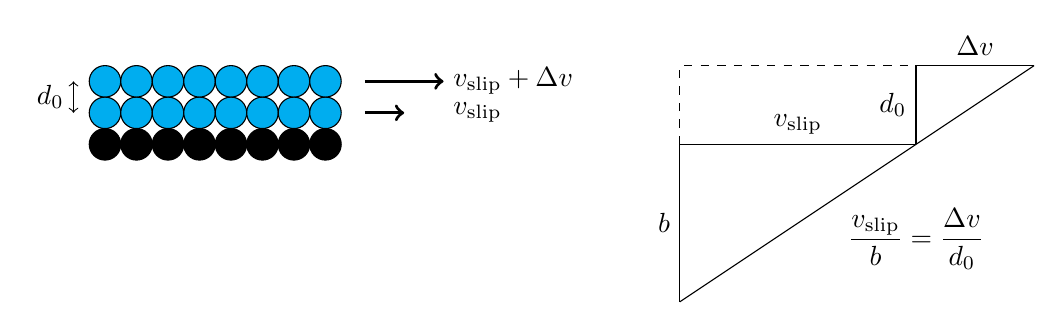
\begin{tikzpicture}
\foreach \x in {1,2,...,8}{
    \draw[fill] (\x*0.4,0) circle (2mm);
    \draw[fill=cyan] (\x*0.4,0.4) circle (2mm);
    \draw[fill=cyan] (\x*0.4,0.8) circle (2mm);
    }
    
\draw[->,very thick] (3.7,0.4) -- ++(0.5,0);
\draw[->,very thick] (3.7,0.8) -- ++(1,0);
\node at (4.7,0.4)[right] {$v_{\mathrm{slip}}$};
\node at (4.7,0.8)[right] {$v_{\mathrm{slip}} + \Delta v$};

\draw[<->] (0,0.4) -- node[left]{$d_0$} ++(0,0.4);

\coordinate (orig) at (7.7,0);
\draw (orig) -- node[above]{$v_{\mathrm{slip}}$} ++(3,0);
\draw (orig) -- node[left]{$b$} ++(0,-2);
\draw (orig) ++(3,0) -- node[left]{$d_0$} ++(0,1) -- node[above]{$\Delta v$} ++(1.5,0);
\draw (orig) ++(0,-2) -- ++(4.5,3);
\draw[dashed] (orig) -- ++(0,1) -- ++(3,0);

\coordinate (eqn) at (10.7,-1.2);
\node at (eqn) {$\displaystyle \frac{v_{\mathrm{slip}}}{b} = \frac{\Delta v}{d_0} $};

\end{tikzpicture}
\caption{Deriving a slip length from a molecular slip experiment.} \label{B&M}
\end{figure}

The similar triangles relation and the force balance equation give us:
\begin{equation}
v_{\mathrm{slip}} = \frac{b}{d_0} \Delta v
\qquad \text{and} \qquad
v_{\mathrm{slip}} = \frac{\mu_{ll}}{\mu_{ls}} \Delta v
\end{equation}
Therefore:
\begin{equation}
b = \frac{\mu_{ll}}{\mu_{ls}} d_0
\end{equation}
Plugging in the numbers yields:
\begin{equation}
b = \frac{1}{18} 0.95 \; \text{nm} = 0.05 \; \text{nm}
\end{equation}

If the data and model are correct, then Becker and Mugele have detected molecular slip with a slip length approximately 1/20th that of the molecule size.  While small, this non-zero slip length shows that at least in the confined geometry of this experiment, the silicone molecules are not sticking to the walls.

\subsection{Conclusions}

These modern, sophisticated experiments investigate slip on atomically flat --- rms roughness $< 1$ nanometer --- solid surfaces, with efforts made to reduce contamination by nanobubbles.  They show no slip on hydrophilic surfaces. For the hydrophobic case, an undeniable intrinsic slip length is present. Two different particle velocimetry studies put an upper limit on intrinsic slip length on the order of 100 nm.  Four different techniques produce results consistent with a slip length in the range $18 \pm 6$ nanometers, at least for moderate shear rates.

In general, no experiment provides direct evidence of molecular slip in water, but these experiments eliminate various confounding factors, leaving molecular slip as a distinct possibility.

\section{Theoretical Intrinsic Slip}

Theoretical arguments for or against slip are somewhat thin on the ground. Computer experiments, in the form of molecular dynamics (MD) simulations, form the backbone of theoretical work.

\subsubsection{Molecular Dynamics}

Molecular Dynamics simulations involve the computer simulation of systems of particles governed by Newtonian mechanics.  Each particle has a position and momentum, and a net force on it due to the interaction with neighbouring particles. Time is sliced into discrete timesteps. At each timestep, the force on each particle is calculated, then the (instantaneous) acceleration, then the resulting translation. Then the position of each and every particle is updated simultaneously, using the calculated translations. The process is then repeated at the next timestep.

The technique is rightly called a computer \emph{experiment}, since the global behaviour is not predictable in advance.  Emergent phenomena such as melting, crystallization, annealing, etc. have been very successfully studied with MD.

Molecular Dynamics simulations differ in their choice of interaction. A very popular choice is the Lennard-Jones interaction, because it is computationally cheap and physically sound: the interaction features an equilibrium distance $\sigma$ between the the particles, a strong repulsion at shorter distances, and a weak attraction at longer distances.  This models dipole-dipole Van der Waals forces quite well.

\vspace*{1em}

Since the power of MD studies depends on Moore's Law, the first serious MD study of the fluid boundary condition appeared in 1990, a paper % in Phys. Rev. A 
by Thompson and Robbins \cite{ThompsonRobbins1990}.
This featured a Lennard-Jones fluid under Couette shear, in conditions equivalent to a compressed fluid about 30\% above melting temperature. This was a qualitative study of the effects of varying two parameters: the wall-fluid interaction strength, \ewf, and the wall \emph{density.}

The wall is composed of stationary atoms. The separation between them can be arbitrarily set to any fraction or multiple of $\sigma$. The wall density is the inverse of separation distance. As the wall density tends to infinity, (separation diminishes to zero), the wall structure asymptotes to a flat plane. In this case, the force between fluid atom and wall is always \emph{perpendicular} to the wall. 
%Thus, the bounce of atoms off the wall will be \emph{specular reflection} --- no change in tangential momentum.  
With no tangential component, the force cannot change the tangential momentum of an incident particle.  This is the case of perfect slip, as shown in Figure (\ref{specular}).
%See Figure (\ref{specular}). This is the case of perfect slip; no transfer of tangential momentum. 
Thompson \& Robbins confirm that perfect slip holds, regardless of the strength of \ewf.


\begin{figure}[ht]
\centering
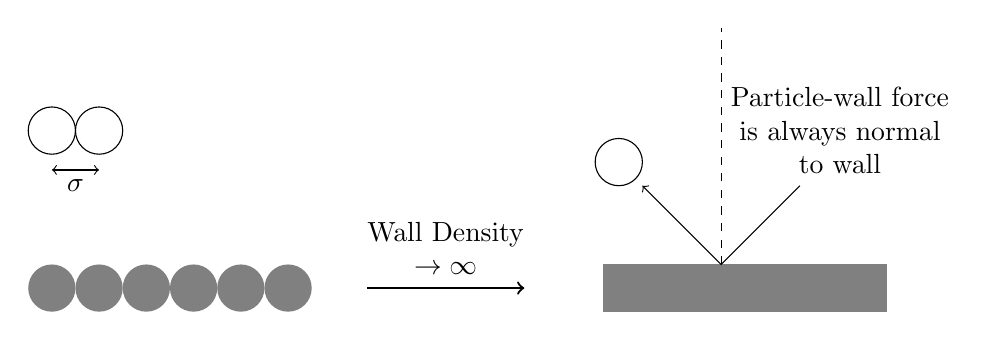
\begin{tikzpicture}
\renewcommand{\baselinestretch}{1.00}

\foreach \x in {0,1,2,3,4,5}
     \fill[color=gray] (\x*0.6,0) circle (3 mm);

\draw (0,2) circle (3 mm);
\draw (0.6,2) circle (3 mm);
\draw[<->] (0,1.5) -- node[below]{$\sigma$} +(0.6,0);

\draw[->, thick] (4,0) -- (6,0);
\node at (5,0.5) [align=center] {Wall Density\\ $\rightarrow \infty$};

\fill[color=gray] (7,0.3) rectangle (10.6, -0.3);
\draw[dashed] (8.5,0.3) -- +(0,3);
\draw[->] (9.5,1.3) -- (8.5,0.3) -- (7.5,1.3);

\draw (7.2,1.6) circle (3 mm);

\node at (8.5,2) [align=center, right] {Particle-wall force\\ is always normal \\ to wall};
 %{Tangential Momentum\\ Same After Collision};
\end{tikzpicture}
\caption{Infinite density of wall atoms leads to perfect slip.} \label{specular}
\end{figure}

\clearpage
As the wall density decreases, the wall gains some `texture', and fluid atoms can be given a sideways kick by the peaks of the wall.  Momentum transfer is now possible, and perfect slip no longer holds.
When the wall density is equal to fluid density, (wall atom separation is $\sigma$), Thompson \& Robbins observe the no-slip condition. At equal density, fluid atoms can attach epitaxially to the wall.  If $\ewf$ is strong enough, one or two layers of fluid atoms lock to the wall.  This is illustrated in Figure (\ref{epitaxial}).

\begin{figure}[ht]
\centering
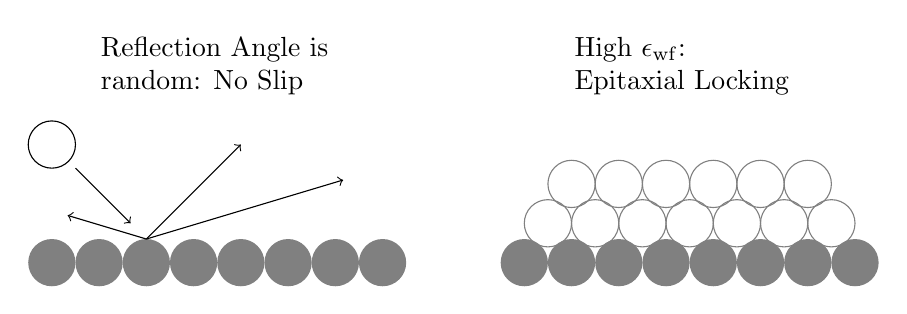
\begin{tikzpicture}
\renewcommand{\baselinestretch}{1.00}

\foreach \x in {0,1,2,3,4,5,6,7, 10,11,12,13,14,15,16,17}
     \fill[color=gray] (\x*0.6,0) circle (3 mm);

\foreach \x in {10,11,12,13,14,15,16}
     \draw[color=gray] (\x*0.6 + 0.3,0.5) circle (3 mm);
 
\foreach \x in {10,11,12,13,14,15}
     \draw[color=gray] (\x*0.6 + 0.6,1) circle (3 mm);
     
\node at (8,2.5)[align=left] {High $\epsilon_{\mathrm{wf}}$:\\ Epitaxial Locking};
         
\node at (0.5,2.5)[right,align=left] {Reflection Angle is\\ random: No Slip};

\draw     (0,1.5) circle (3 mm);
\draw[<-] (1.0,0.5) -- +(-0.7,0.7);
\draw[->] (1.2,0.3) -- +(1.2,1.2);
\draw[->] (1.2,0.3) -- +(2.5,0.75);
\draw[->] (1.2,0.3) -- +(-1,0.3);

\end{tikzpicture}
\caption{Wall atom separation equal to fluid atom diameter.} \label{epitaxial}
\end{figure}


At a wall density of 2.52 times the fluid density (solid atom separation is 0.397 $\sigma$), Thompson \& Robbins found that fluid layering was reduced, and slip increased. At higher \ewf, however, the fluid atoms again formed a close-packed layer, but with a periodic structure that was a harmonic of the wall structure. At the highest \ewf, the fluid atoms locked epitaxially to the wall, in a state of elastic strain.
See Figure (\ref{elastic}).

\begin{figure}[ht]
\centering
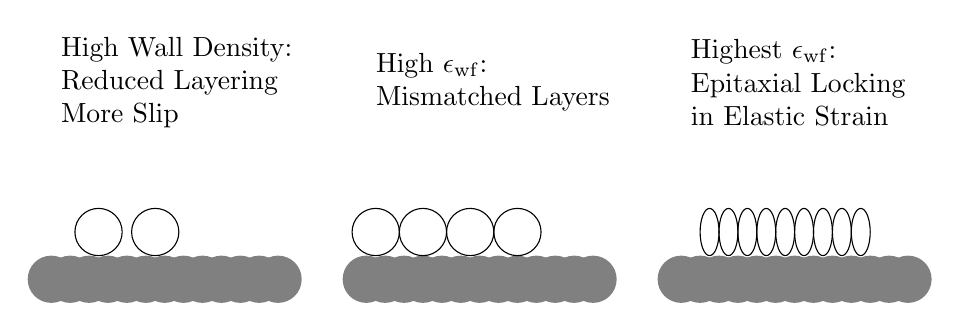
\begin{tikzpicture}
\renewcommand{\baselinestretch}{1.00}

\foreach \d in {0,4,8}
    \foreach \x in {0,1,2,3,4,5,6,7,8,9,10,11,12}
        \fill[color=gray] (\x*0.24 + \d,0) circle (3 mm);

\foreach \d in {2,5}
    \draw (0.12 + 0.24*\d, 0.6) circle (3 mm);

\node at (0,2.5)[right,align=left] {High Wall Density:\\Reduced Layering\\More Slip};

\foreach \x in {0,1,2,3}
    \draw (4.12 + 0.6*\x, 0.6) circle (3 mm);

\node at (4,2.5)[right,align=left] {High $\epsilon_{\mathrm{wf}}$:\\Mismatched Layers};

\foreach \x in {1,2,3,4,5,6,7,8,9}
    \draw (8.12 + 0.24*\x, 0.6) ellipse (1.2mm and 3mm);

\node at (8,2.5)[right,align=left] {Highest $\epsilon_{\mathrm{wf}}$:\\
Epitaxial Locking\\ in Elastic Strain};

\end{tikzpicture}
\caption{Wall atom separation 0.4 $\times$ fluid atom diameter.} \label{elastic}
\end{figure}

\vspace*{1em}

\clearpage
Following this qualitative work, Thompson and Troian report some quantitative results from very similar Lennard-Jones simulations in 1997 %a 1997 Nature article
 \cite{ThompsonTroian1997}. 
Again they vary the wall density $\rho_{\mathrm{wf}}$ and \ewf, (as a fraction of $\epsilon$, the fluid-fluid interaction strength) as well as $\sigma_{\mathrm{wf}}$, the equilibrium distance of wall and fluid atoms. Slip lengths in units of $\sigma$ are calculated for various regimes, and appear in Table (\ref{tnt}).

\begin{table}[h]
\centering
\caption{Slip lengths (units of $\sigma$) for various simulation parameters.} \label{tnt}
\begin{tabular}{l l l l}
\ewf & $\sigma_{\mathrm{wf}}$ & $\rho_{\mathrm{wf}}$ & $b$ \\
0.6  & 1.0                    & 1                    & 0 \\
0.1  & 1.0                    & 1                    & 2 \\
0.6  & 0.75                   & 4                    & 4 \\
0.4  & 0.75                   & 4                    & 8 \\
0.2  & 0.75                   & 4                    & 18 \\
\end{tabular}

\end{table}

Now, $\ewf < \epsilon$ means that a fluid atom is more attracted to other fluid atoms than to the wall.  This could imply hydrophobicity; in general, hydrophobicity increases as $\ewf$ decreases. Hence, the data show that if epitaxial locking is easy, then slip is suppressed, even for a mildly hydrophobic surface. Likewise, the data show that if the density of stable attachment sites is too high for epitaxial locking, then slip results.

But the real story is the shear dependence of slip. The fluid is in a Couette flow regime, with top and bottom surfaces moving with equal and opposite velocities.  At low shear rates, the slip length is a constant plateau, but at some critical shear rate, the slip length diverges. %, i.e. goes berserk heading for infinity. 
The critical shear rate depends on the regime.  Interestingly, if the shear rates are normalised to their critical shear rate, and the slip lengths normalised to their plateau value, then the slip length versus shear rate data for all regimes lie \emph{on a single curve.}

Thompson \& Troian attempt to explain this ``remarkable collapse of the data" with a single parameter $R$ describing the roughness of the potential surface. A test particle at a fixed height experiences a potential $\phi(x,y)$. Define $A$ as the area integral of $\phi(x,y)$, and $A_{\infty}$ as the area integral of the limiting case of a flat plane (infinite atom density). Then

\begin{equation}
R = \frac{A}{A_{\infty}} - 1
\end{equation}

With a wall moving at velocity $v$, a test particle experiences perfect slip for $v>v_{c}$, some critical velocity. They find that $v_{c}$ scales as $R^{1/2}$ for a wide range of parameters. In the real fluid (with hundreds of particles) they find $v_{c}$ scales as a power of $R$ with an exponent close to $3/4$.

Thompson \& Troian think it is reasonable to assume that $v_{c}$ is set by the liquid-solid interaction timescale, so that increasing density should lead to larger $v_{c}$.  They are surprised to find the reverse.

But this is an odd expectation.  Assuming that the average approach velocity of impacting particles remains the same, a faster-moving or more dense surface surface increases the probability that the particle will interact with a peak.  Since the peaks are the `flattest' parts of the surface, the particle has a greater chance of being deflected by a force that is closer-to-normal to the surface plane, which will not change the tangential momentum of the particle as much.  This implies increased slip.
%In the same way, an electric fan seems `solid' to the inquisitive fingers of a child.
\vspace*{1em}

Barrat and Bocquet \cite{BarratBocquet1999} study flow in both Poiseuille and  Couette regimes, using a Lennard-Jones fluid with an additional $c_{ij}$ parameter:

\begin{equation}
v_{ij} = 4 \epsilon \left[ \left( \frac{\sigma}{r}\right)^{12}
 - c_{ij} \left( \frac{\sigma}{r} \right)^{6} \right]
\end{equation}


They use $c_{FF} = 1.2$ for fluid-fluid interactions, making the fluid more cohesive than the usual Lennard-Jones fluid. They tweak the wetting properties via the $c_{FS}$ fluid-solid parameter.  There are several ways to calculate the contact angle from this parameter.  The most accurate way gives $c_{FS}=0.5 \rightarrow \theta= 140^{\circ}$ and $c_{FS} = 1.0 \rightarrow \theta = 90^{\circ}$.

A hydrophobic liquid ($\theta = 140^{\circ}$) requires a pressure $P_{0}$ to pump it down the pipe. % (to overcome Laplace pressure).
 At high pressure, $P/P_{0}=16.4$, the fluid exhibited the same higher-density layering at the wall as seen in hydrophilic liquids.  At a lower pressure, %$P/P_{0}$,
  the fluid showed a \textbf{strong density depletion} near the wall.  The slip length varied tremendously over this pressure range: from $b = 8\sigma$ for $P/P_{0} = 16.4$ to over $40\sigma$ for $P/P_{0} \sim 0$.

Less hydrophobic fluids showed less slip, and less pressure dependence. A $c_{FS}>0.7$ ($\theta \leq 120^{\circ}$) gave slip lengths of a couple of $\sigma$ only.

Note that the position of the hydrodynamic boundary was treated as an adjustable parameter.  It turned out to be located one atom width into the liquid.  The arbitrary nature of the boundary position was not fully appreciated by the experimental community until almost 10 years after this sort of theoretical paper.

\subsubsection{Correlation Function Tuned by Molecular Dynamics}

In a theoretical study \cite{BocquetBarrat1994}, Bocquet and Barrat start by constructing a phenomenological model of a fluid: Each infinitesimal volume of fluid has a \emph{momentum.} This momentum field is subject to fluctuations, which quickly dissipate, obeying the diffusion equation. Further, any pressure gradient is proportional to the gradient of momentum divergence. Incorporating density $\rho_0$, shear viscosity $\eta$, bulk viscosity $\xi$, and dividing through by the volume element to get a momentum \emph{density,} $\vec{j}(\vec{r},t)$, in the bulk:
\begin{equation}
 \partial_{t} \vec{j}+\nabla P - \frac{\xi+\eta/3}{\rho_{0}}\nabla
 [\nabla \cdot \vec{j}] - \frac{\eta}{\rho_{0}} \nabla^{2} \vec{j} = 0
\end{equation}
And on the boundary, Navier slip holds:
\begin{equation}
\vec{j}_{\parallel} = b_{\mathrm{wall}} \frac{\partial}{\partial \vec{n}}
 \vec{j}_{\parallel} , \;\;\;\;\; \vec{j}_{\perp} = 0
\end{equation}
Bocquet \& Barrat now consider a fluid contained between two $x,y$ planes separated by distance $h$. Slip lengths $b_{0}$ and $b_{h}$ hold on the lower and upper planes, respectively.

A great simplification is to introduce the `transverse momentum density':

\begin{equation}
j_{x}(z,t) = \frac{1}{L_{x}L_{y}} \int \int dx dy \; j_{x}(\vec{r},t)
\end{equation}
And similarly for $j_{y}(z,t)$.

With the pressure gradient essentially integrated out, this field obeys the diffusion equation + Navier slip conditions:
\begin{gather}
\left[ \partial_{t} - \frac{\eta}{\rho_{0}} \partial_{z}^{2} \right]
j_{x}(z,t) = 0
\\
j_{x}(z,t)|_{z=z_{0}} = b_{0} \partial_{z} j_{x}(z,t)|_{z=z_{0}} , \;\;\;\
\;\;  j_{x}(z,t)|_{z=z_{0}+h} = -b_{h} \partial_{z} j_{x}(z,t)|_{z=z_{0}+h}
\end{gather}

Work with the time-dependent correlation function:

\begin{equation}
C(z,z',t) = \left< j_{x}(z,t), j_{x}(z',0) \right>
\end{equation}
where angle brackets denote a thermodynamic average.

Finally, this equilibrium correlation function also obeys the diffusion and Navier slip equations:

\begin{gather}
\left[ \partial_{t} - \frac{\eta}{\rho_{0}} \partial_{z}^{2} \right]
C(z,z',t) = 0 \quad :\;\; 0<z<z_{0}+h 
\\
C(z,z',t)|_{z=z_{0}} = b_{0} \partial_{z} C(z,z',t)|_{z=z_{0}}
\\
C(z,z',t)|_{z=z_{0}+h} = -b_{h} \partial_{z} C(z,z',t)|_{z=z_{0}+h}
\end{gather}
There is a general solution (details omitted):

\begin{equation}
C(z,z',t) = f(b_{0}, b_{h}, h)
\end{equation}

That is, the correlation function is a function of \emph{slip length} and \emph{channel width.} The parameter `channel width' is equivalent to `effective position of the boundary condition'.  Bocquet \& Barrat note that in Couette flow, the two parameters are not independent, but in general may be.

Now, one can directly observe a molecular dynamics simulation, and calculate the correlation function from the atomistic dynamics that occur in the simulation. Bocquet \& Barrat carry out an equilibrium MD simulation --- no shear or pressure, just thermal motion --- and compute the correlation function.  The parameters of the theoretical correlation function are adjusted to fit the MD correlation function.
%tweaked until it best fits the MD correlation function.

Thus, a slip length and effective boundary position are derived from MD, without inducing and measuring velocities, therefore eliminating  shear dependence from the slip effect.

The first MD experiment used a repulsive-only fluid/wall interaction -- a `soft sphere' model. The wall had a corrugation with wavelength of $1 \sigma$, and a varying amplitude.  Results for various amplitudes are shown in Table (\ref{t2}).


\begin{table}[h]
\centering
\caption{Slip lengths for different amplitudes of wall corrugation.} \label{t2}
\begin{tabular}{lll}
Amplitude      & Slip Length      & BC Position \\
0  (flat)      & $\infty$         & 1.60 \\
0.01           & $40 \pm 2.5$     & 1.60 \\
0.02           & $7.20 \pm 0.05$  & 1.60 \\
$>0.03$        & $0.00 \pm 0.02$  & 1.60 \\
\end{tabular}
\end{table}

The remarkable result is that even a tiny corrugation --- depth 0.03 $\sigma$ --- is enough to completely suppress slip. Also, the hydrodynamic BC is located about one atom width inside the fluid.

A second Lennard-Jones MD simulation with a corrugation depth of 0.2 $\sigma$ was done.  Particles locked epitaxially to the solid, with zero slip, and a BC located two atom widths inside the fluid.

As a final test, Bocquet \& Barrat do a conventional Couette flow MD simulation, extracting velocity profiles to infer slip lengths. The results agreed with the equilibrium method.


\clearpage
\subsubsection{Depletion Layer and Drainage Force}
In a landmark paper from 1995 \cite{Vinogradova1995}, Olga Vinogradova studied the `drainage of a thin liquid film confined between hydrophobic surfaces'. The results are in two main parts.

\paper{The Boundary Conditions on the Hydrophobic Surface:}
Vinogradova looks at the two candidates for intrinsic slip: molecular slip and apparent slip.
She notes that molecular slip was first proposed by Tolstoi back in 1952; his theories were revisited by Blake in 1990, who predicted the slip effect on flow rate in a capillary.  These predictions sometimes matched experiment, but Ruckenstein and Rajora in 1993 noted that the implied surface diffusion coefficients are several orders of magnitude larger than those observed even for gases.

Having found evidence for molecular slip wanting, she considers apparent slip.  A `gas gap' has been suggested as the cause, but this is not experimentally confirmed. Another model of apparent slip is the decrease in viscosity in a boundary layer close to the hydrophobic surface. Crucially, she states: ``this fact follows from numerical simulation data, as well as from the direct experimental results obtained by the blowoff method. (Derjaguin \emph{et al} 1993)". From this firm foundation, Vinogradova notes that if the boundary layer of thickness $\delta$ has an average viscosity $\mu_{\mathrm{slip}}$, smaller than the bulk viscosity $\mu_{\mathrm{bulk}}$, then an order of magnitude estimate of apparent slip length is:

\begin{equation}
b= \delta \left( \frac{\mu_{\mathrm{bulk}}}{\mu_{\mathrm{slip}}} - 1 \right)
\end{equation}

%This is of course would be well defined only if $\delta$ and $\mu_{\mathrm{slip}}$ were known.

This model covers the case of bubbles on the surface, and Vinogradova observes that much experimental slip may be due to dissolved gas, causing bubbles to form on the surface or in microcavities.

\clearpage
\paper{Solution of the Drainage Problem:}
Vinogradova considers two perfectly spherical (no roughness) solids being squeezed together at (instantaneous) velocity $v$ in a Newtonian fluid of viscosity $\mu$. The two spheres have radii $R_{1}$ and $R_{2}$, and slip lengths $b$ and $b(1+k)$ on their surfaces, respectively. 
%After a lovely piece of classical mathematical physics, she 
She derives a formula for the drainage force
$F_{z}$ in terms of separation $h$:

\begin{equation}
F_{z} = - \frac{6 \pi R_{e}^{2} \mu v}{h} f^{*}
 \;\;\;\; \mathrm{where}\;\;\;R_{e} = \frac{R_{1}R_{2}}{R{1}+R_{2}} = 
 \frac{R_{1}}{\frac{R_{1}}{R_{2}} + 1}
\end{equation} 

 In the limiting case of a hydrophobic sphere interacting with a similar one:
 
\begin{equation}
f^{*} = (2)\frac{h}{6b} \left[ \left(1 + \frac{h}{6b} \right)
 \ln \left(1 + \frac{6b}{h} \right) - 1 \right]
\end{equation}
Note that $R_{e} = R_{1}$ in the case of a sphere approaching a flat plane ($R_{2}=\infty$).

This formula has been used by the experimental community in all subsequent drainage force experiments.

\subsubsection{Depletion Layer as a Gas Layer}

%In a wonderfully readable little paper from 2002 in Langmuir
In paper from 2002 in Langmuir \cite{deGennes2002}, de Gennes derives the slip length expected of a hypothetical gas layer.  De Gennes finds the then-recent very high experimental slip lengths ``unexpected and stimulating."  (These experiments are now suspected of being contaminated with bubbles; de Gennes is thus prescient in his gas layer theory.) ``This led us to think about unusual processes which could take place near a wall.  In this Letter, we discuss one (remote) possibility: the formation of a gaseous film at the solid/liquid interface.

``The source of the film is unclear: when the contact angle is large ($\theta \rightarrow 180^{\circ}$), a type of flat bubble can form at the surface with a relatively low energy.  But this energy is still high compared to the thermal energy $k_{B} T$."

With these caveats stated, de Gennes derives the slip length expected for a bulk fluid of viscosity $\eta$, sliding over a gas layer of density $\rho$, and uniform thickness $h$. Layer thickness $h$ is assumed to be greater than the molecule size, but smaller than the mean free path in the gas.

Unfortunately, there are a few issues: there seem to be several typographical errors, and the result is stated in terms of the somewhat unfamiliar $\bar{v}_{z}$, which is  %apparently 
defined as the mean \textbf{absolute value} of the normal component of gas particle velocity (the simple mean is zero).  To resolve the inconsistencies, and restate the result in a more standard way, in Appendix A we derive the result from scratch, in terms of the mean \emph{speed} in the gas, $\bar{v}$.  We find:
\begin{equation}
b = \frac{4 \eta}{\rho \bar{v}}
\end{equation}
(We show that this is equivalent to the result of de Gennes.)

Note that $b = 4 \eta/ \rho \bar{v}$ is the slip length parameter found in the boundary condition located at the \textbf{bottom of the fluid.}  If $b$ is instead regarded as a property of the \emph{solid} surface, then the gas layer thickness $h$ must be subtracted.  We shall see that this is negligible:

Plugging in typical values: $\rho$ = 1 kg/m$^{3}$, $\bar{v}$ = 476 m/s, $\eta$ = $10^{-3}$ kg/ms, we get $b$ = 8 $\mu$m. De Gennes: ``Thus, a gas film can indeed give a very large slip length.  Our calculation assumed complete thermalization at each particle/boundary collision.  If we had some nonzero reflectance (especially on the solid surface), this would increase $b$ even more."

De Gennes notes that the amount of gas required is very small, but that a ``process which could generate such films remains obscure."  Serendipitously, the very next year, Andrienko \emph{et al} proposed an abstract description of just such a process.

\clearpage
\subsubsection{Phase Separation causing a Depletion Layer}

The depletion layer theory of slip was given another boost 
% by some fairly abstract theorising
 by Andrienko \emph{et al} in a 2003 paper \cite{Andrienko2003}.  Rather than focusing on what the low-viscosity boundary \emph{is,} they take an agnostic, abstract approach: They considered a toy model of a generic admixture of two different fluids, whose viscosities differ by the (arbitrary) ratio 1:3.  A `phase field' approach was used, in which an order parameter $\phi$ varies over space.  Here, $\phi$ was the fraction of low-viscosity fluid in an infinitesimal volume.

The unmixing of the fluid is driven by energy.  Andrienko \emph{et al} start with a free energy functional --- the semigrand potential. With this functional set up, they consider the physical case of Couette flow between two fairly close plates. Variation of the functional yields an Euler-Lagrange equation and a boundary condition.

%\begin{gather}
% k^{2} \frac{\partial^{2}\phi}{\partial z^{2}} + 
%\frac{1}{2}T\ln \frac{1+\phi}{1-\phi} + \mu = 0
%%\end{equation}
%\\
%%\begin{equation}
%\pm k \frac{\partial \phi}{\partial z} + h + \gamma \phi|_{z= \pm L/2} = 0
%\end{gather}
%Where $k$ is inexplicably undefined, $T$ is temperature, $\mu$ is chemical potential, $h$ measures attractiveness of the surface to the low-viscosity fluid, and surface coupling $\gamma$ captures the fact that a molecule on the surface has fewer neighbours than a molecule in the bulk.

These equations were solved numerically using the relaxation method. With the $\phi$ field solution, the viscosity field was obtained by simply assuming that viscosity is a linear combination of the pure viscosities. Finally the Couette flow field was solved for the viscosity field.

The big result is that above a certain temperature, a layer of the low-viscosity fluid suddenly forms on the surface.  Andrienko \emph{et al} call this a `prewetting transition'.  This causes the sudden emergence of a significant slip length.  As temperature increases above this critical temperature, more mixing occurs, reducing the viscosity contrast, thus reducing slip length.

Andrienko \emph{et al} believe this mean-field toy model to be valid for liquid-gas systems, binary mixtures, and polymer mixtures in the long wavelength approximation.  Thus, large slip is predicted for those systems.



\clearpage
\section{Conclusions}

%Intrinsic slip certainly exists, on atomically-flat clean surfaces.  Molecular dynamics simulations show a variety of interesting phenomena, including molecular slip, and a depletion layer causing apparent slip.  The depletion layer model is an excellent candidate for a physical explanation.  Intrinsic slip lengths of roughly 20 nanometers are credibly measured. 


There exist a few recent experimental studies confirming intrinsic slip over hydrophobic surfaces, where the solid surface is flat -- less than 1 nm rms roughness -- and care has been taken to minimise contamination by nanobubbles.

The drainage force experiment of Cottin-Bizonne \emph{et al} in 2005 \cite{Cottin-Bizonne2005} featured a resolution of 1 Angstrom for the probe to surface distance.  They found a slip length of $19 \pm 2$ nm.
This is consistent with the particle velocimetry experiments of Joly \emph{et al} of 2006 \cite{Joly2006}, which estimated the diffusion coefficient of unmoving water, thus eliminating issues of shear-induced bubble formation.  The model fitted to the results implied a slip length of $18 \pm 5$ nm.
More conventional particle velocimetry experiments by Huang \emph{et al} in 2006 \cite{Huang2006} with degassed water showed a shear-dependent slip length. Given the experimental uncertainties, they present an upper limit of 150 nm for the slip length.
Vinogradova in 2009 \cite{Vinogradova2009} noted that shear flow can increase the effective diffusivity of particles in the velocimetry experiment. Her calculations from her experimental results take this into account, yielding a slip length of no more than 80 - 100 nm for hydrophobic capillaries.

On the theoretical side, intrinsic slip is observed in molecular dynamics simulations \cite{ThompsonRobbins1990}, \cite{ThompsonTroian1997}, \cite{BarratBocquet1999}, \cite{BocquetBarrat1994}.  At sufficiently low pressure in the liquid, Barrat and Bocquet observe a depletion layer -- a layer of lower-than-bulk density liquid at the solid surface \cite{BarratBocquet1999}.  The effect of a density layer was explored by de Gennes in 2002 \cite{deGennes2002}.  He shows that observed slip effects are explainable by a gas layer one or two atoms thick at the surface.  Andrienko \emph{et al} in 2003 \cite{Andrienko2003} showed a model of a binary mixture of high and low viscosity fluids. In the model, above a certain temperature, a depletion layer spontaneously formed on the surface.

In the next chapter, we turn to flow over mixed-slip surfaces, 
where the intrinsic slip length is different on different parts of the surface.   

\iftoggle{compilealone}
    {
    \bibliography{Lund_Thesis.bib}
    \bibliographystyle{plain}
    }
    
\end{document}

% This is not necessarily in the format for a VUW thesis chapter.

\documentclass[a4paper]{report}

\usepackage{amssymb, amsmath}
\usepackage{tikz}
\usetikzlibrary{calc}

%\usepackage{marvosym}


\title{Chapter 3: Mixed Slip Flow}
\author{Nat Lund}

\newcommand{\beff}{\ensuremath{b_{\mathrm{eff}}}}
\newcommand{\bhigh}{\ensuremath{b_{\mathrm{high}}}}
\newcommand{\blow}{\ensuremath{b_{\mathrm{low}}}}
\newcommand{\phislip}{\ensuremath{\phi_{\mathrm{slip}}}}
\newcommand{\phisol}{\ensuremath{\phi_{\mathrm{solid}}}}
\newcommand{\sigsol}{\ensuremath{\sigma_{\mathrm{solid}}}}
\newcommand{\gamsol}{\ensuremath{ \dot{\gamma}_{\mathrm{solid}} }} 

\newcommand{\sep}{\begin{equation*} \star \end{equation*}}

\newcommand{\paper}[1]
         {\colorbox[gray]{0.8}{ \textsc{#1}}
         
         }

\begin{document}
\maketitle

If water flows over a surface covered with air pockets, then the water experiences a boundary that is partly fresh air, and should experience reduced drag.  That is, the air-water interface should exhibit a large slip length, and such air-pocketed  surface should have a larger effective slip length than the unadorned surface.  It is tempting to accept this as self-evident, and immediately proceed to finding an effective slip length in terms of the intrinsic slip lengths.  However, there exist experimental results in which such a surface has a \emph{reduced} effective slip compared to the pure surface.  Furthermore, there are claims that roughness both increases \emph{and} decreases slip.  The paradox in these findings is ultimately resolved by taking appropriate care in defining the location of the $z=0$ plane.  Since this a key part of any mathematical model, we shall spend this chapter looking at the nuances of this issue.  We trace an approximate historical development of results for flow over heterogeneous surfaces: that is, surfaces that are rough, or mixed-slip surfaces,  whose intrinsic slip length varies across the surface.

%While the boundary condition in classical fluid mechanics is homogeneous (`no slip'), and we are satisfied that fluid slip %can indeed occur on an atomically flat homogeneous surface, we now turn our attention to \emph{mixed-slip} surfaces.
%That is, surfaces that are heterogeneous --- where the intrinsic slip length is different on different parts of the %surface.

\section{Mixed Slip Surfaces}

While there could in principle be an infinite variety of mixed-slip surfaces, only two broad classes are important.  This is because physical mixed-slip surfaces almost always feature a liquid-\emph{air} interface, along with the the more familiar liquid-solid interface.  And there are two canonical configurations: superhydrophobic, and nanobubbles.

\subsection{Superhydrophobic Surfaces}

Recall that when a droplet of water sits on a surface, a contact angle $\theta$ is defined:

\begin{center}
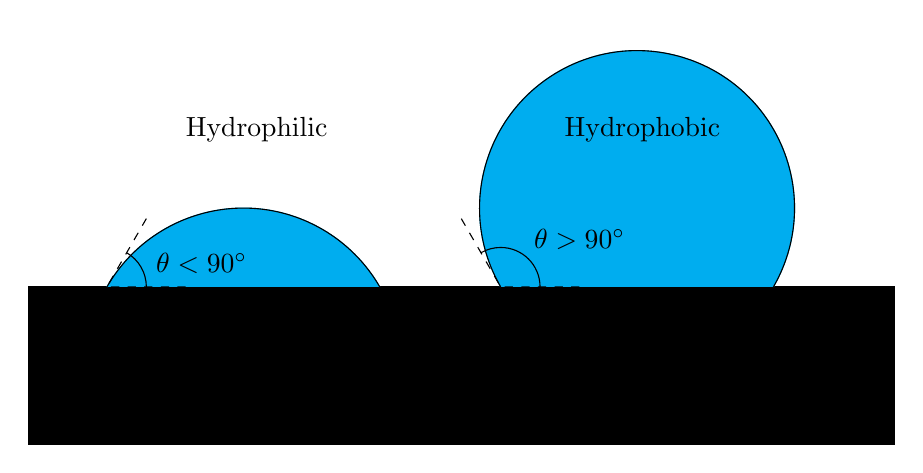
\begin{tikzpicture}
\filldraw (-1,0) rectangle +(11,-2); 

\filldraw[color=cyan] (0,0) arc (150:30:2);
\draw (0,0) arc (150:30:2);

\draw[dashed] (1,0) -- (0,0) -- (0.5,0.866);
\draw (0.5,0) arc (0:60:0.5);
\node at (0.5,0.3)[right] {$\theta < 90^{\circ}$};

\filldraw[color=cyan] (5,0) arc (210:-30:2);
\draw (5,0) arc (210:-30:2);

\draw[dashed] (6,0) -- (5,0) -- +(-0.5,0.866);
\draw (5.5,0) arc (0:120:0.5);
\node at (5.3,0.6)[right] {$\theta > 90^{\circ}$};

\node at (1.9,2) {Hydrophilic};
\node at (6.8,2) {Hydrophobic};

\end{tikzpicture}
\end{center}

Usually, a surface is defined as \emph{hydrophobic} when the contact angle is more than $90^{\circ}$.  This means that the water molecules are more attracted to each other than they are to the surface. (If $\theta < 90^{\circ}$, the surface is \emph{hydrophilic}.  If $\theta \sim 0^{\circ}$, then \emph{complete wetting} occurs: the water spreads out as far as it can.)

Tiny, micron or nanometer scale pillars can be constructed out of hydrophobic material.  A collection of theses hydrophobic nanopillars can be affixed to a suitable substrate, forming a `nanoforest'.  (Or, more practically, a nanoforest can be constructed, then chemically treated to become hydrophobic.)  If a water droplet is placed on top of the nanoforest, two curious things happen:  First, the droplet sits on the tops of the nanopillars, supported by surface tension.

\begin{center}
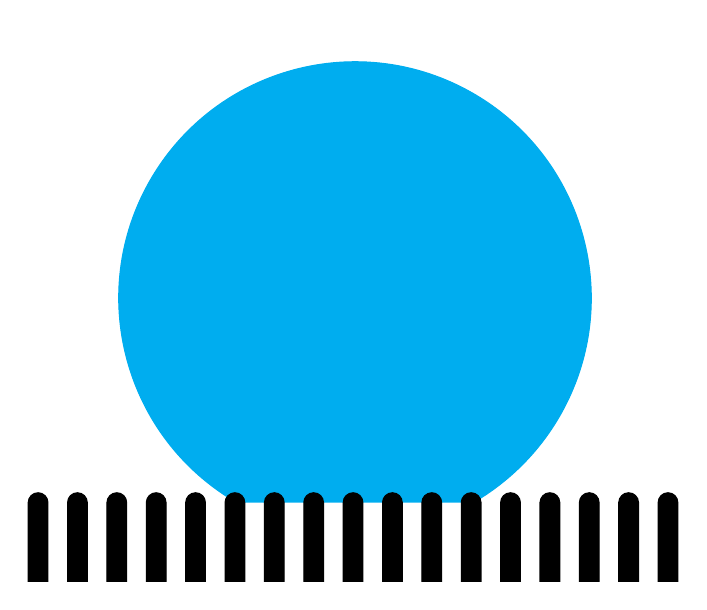
\begin{tikzpicture}

\filldraw[color=cyan] (3.15,1) arc (240:-60:3);

\foreach \x in {1,2,...,17}
{ \filldraw (\x/2,0) rectangle +(0.25,1) arc (0:180:0.125); }

\end{tikzpicture}
\end{center}

Second, the apparent contact angle is very large.  This second effect is caused by the fact that at the point where the contact line is located, the solid surface is at an angle to the plane of the nanoforest.

\begin{center}
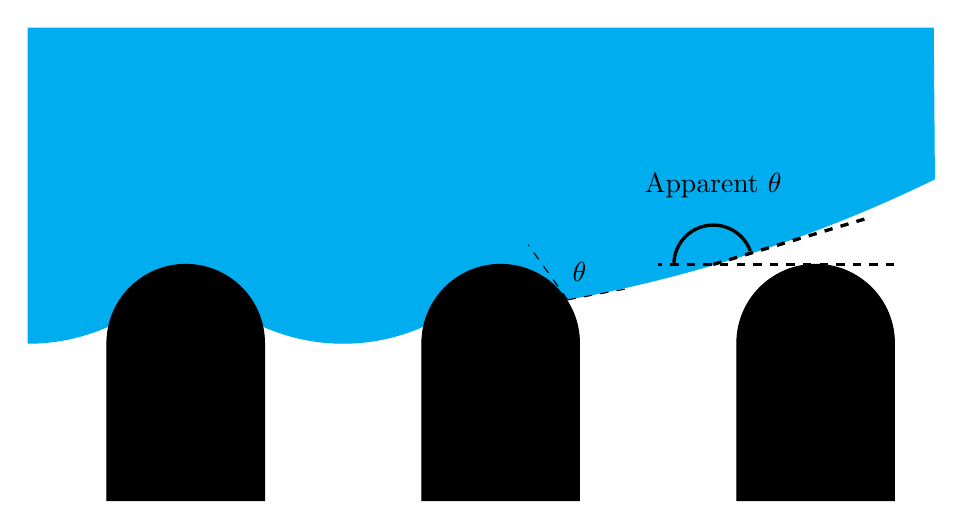
\begin{tikzpicture}

\filldraw[color=cyan] (10.5,6) -- (-1,6) -- (-1,2) arc (270:300:2.5)  -- +(1.5,0) arc (240:300:2.5) -- 
(5.75,2.54)  arc (-80:-64:18);

\foreach \x in {0,1,2}
\filldraw (\x*4,0) rectangle +(2,2) arc (0:180:1);

\draw[dashed] (5.85,2.55) -- +(-0.5,0.7);
\draw[dashed] (5.85,2.55) -- +(0.8,0.15);
\node at (6,2.9) {$\theta$};

\draw[very thick, dashed] (10, 3) -- +(-3,0);
\draw[very thick, dashed] (7.7,3) -- +(2,0.6);
\draw[very thick] (7.2,3) arc (180:20:0.5);
\node at (7.7,4) {Apparent $\theta$};

\end{tikzpicture}
\end{center}

Due to the extremely high contact angle, these nano or micro-structured surfaces are known as \emph{superhydrophobic} surfaces.


\vspace*{1em}
Such surfaces were constructed as early as 1996.  Onda \emph{et al} \cite{Onda1996} discussed the theoretical contact angle of such a surface, and demonstrated a ``super-water-repellent fractal surface'' made of alkylketene dimer, with a remarkable contact angle of $174^{\circ}$.

Enormous contact angles are routinely quoted for static droplets.  The contact angle is slightly different if the droplet is advancing (or retreating).  This hysteresis was studied, for example, by Kusumaatmaja and Yeomans in 2007 \cite{KusumaatmajaYeomans2007}.

But perhaps more interestingly, superhydrophobic surfaces were first observed in nature. The sacred lotus is an aquatic plant (not a water lily, but similar) whose water-repellent qualities have been noted since antiquity.  A passage in the Baghavad Gita states ``One who performs his duty without attachment, ... is unaffected by sinful action, as the lotus is unaffected by water."
In 1993, Barthlott and Neinhuis were taking scanning electron micrographs of the leaf surfaces of some 10,000 plant species.  They noticed that \emph{flat} surfaces always had to be cleaned before examination, while certain rough waxy surfaces did not.  They characterised these self-cleaning surfaces as covered with wax crystalloids ``in a regular microrelief of about 1 - 5 $\mu$m" -- i.e. superhydrophobic.  They describe the cleaning mechanism: Water beads into near-spherical droplets, which easily roll off the leaf.  Dirt particles tend to be hydrophilic, and only weakly bound to the tops of the roughness.  Thus the dirt particles are captured by the water droplets, and move with them off the leaf.  More from antiquity: a Confucian scholar wrote ``I love the lotus, because while growing in mud, it is unstained." In a pair of papers in 1997 \cite{BarthlottNeinhuis1997,NeinhuisBarthlott1997}, Barthlott and Neinhuis describe their studies of what they dub the `lotus effect'.

The image of a droplet supported by thin spikes inspires another metaphor: a Fakir (malnourished Yoga practitioner) sitting on a bed of nails.  David Qu\'{e}r\'{e}'s article `Fakir droplets' gives a very readable summary of the state of affairs in 2002 \cite{Quere2002}.  The quote of relevance to this thesis is the last few sentences of the article: ``On a superhydrophobic solid, however, drops seem to move over a dynamic film of air --- which makes the friction comparable to that experienced by a raindrop falling in air.  But what happens if these textured solids are fully immersed in a pool of water? Will the water still slide on them?  Except for a few controversial studies, this question still remains open, and designers of boats and swimsuits impatiently await an answer."

This question heads a line of research leading to this thesis.


\subsection{Nanobubbles}

In 2001, Tyrrell and Attard discovered what appeared to be nanobubbles on hydrophobic surfaces \cite{TyrrellAttard2001}.  An extract from the abstract of their PRL paper says it all: ``Imaging of hydrophobic surfaces in water with tapping mode atomic force microscopy reveals them to be covered with soft domains, apparently nanobubbles, that are close packed and irregular in cross section, have a radius of curvature of the order of 100 nm, and a height above the substrate of 20 -- 30 nm."  

It had been observed that when two hydrophobic bodies were brought together underwater, at some very close separation, a `hydrophobic force' suddenly pulled them together.  In 2002, Tyrrell and Attard published \cite{TyrrellAttard2002} more AFM images of nanobubbles, and proposed them to be the origin of the `hydrophobic force'.

\begin{center}

\begin{tikzpicture}
\filldraw (0,0) rectangle (10,-2);
\filldraw[color=cyan] (0,0) rectangle (10,4);

\draw[fill=white] (1,0) arc (150:30:1);
\draw[fill=white] (3,0) arc (150:30:0.5);
\draw[fill=white] (5,0) arc (130:50:1.5);
\draw[fill=white] (8,0) arc (150:30:0.8);

\end{tikzpicture}
\end{center}

The question naturally arises: when are nanobubbles present?  Yang and coworkers published in 2007 \cite{Yang2007} an exhaustive experimental study on the factors influencing the formation of nanobubbles, such as temperature, dissolved gases etc.  It turns out that if a surface had been immersed in ethanol before being immersed in water, then nanobubbles are reliably formed.  Using this `solvent exchange' technique, Yang and coworkers were able to do repeatable studies of nanobubbles.  Using infrared spectroscopy, they confirmed the presence of a gas phase 5 -- 80 nm thick at the surface --- i.e. good evidence that the `soft domains' really are nanobubbles.  The pressure in the bubbles was found to be 1.0 -- 1.7 atmospheres, consistent with the Laplace pressure calculated from their radii of curvature.  This low pressure allows nanobubbles of air to remain stable for days.  They find that nanobubbles form much more easily on rough surfaces, sometimes even without the solvent exchange technique.

Crucially, the solvent exchange technique is also a common cleaning technique.  Therefore, nanobubbles may be formed inadvertently in the process of a slip experiment.  Given the further fact that rough surfaces may spontaneously form nanobubbles, the question arises:  How many ostensibly `pure' slip experiments are actually experiments on \emph{mixed-slip} surfaces?

A purpose of the research in this thesis is to give some indication of the effect of such nanobubble contamination on a slip experiment.

\vspace*{1em}
In summary, mixed-slip surfaces tend to fall into the two types described above: either a solid surface interspersed with pockets of air (nanobubble type), or a gas-liquid interface interspersed with islands of solid material (superhydrophobic type).  Thus, a superhydrophobic type surface has a contiguous \emph{air-liquid} interface, while a nanobubble type surface has a contiguous \emph{solid} phase.

In the two-dimensional case, the difference disappears.  \emph{Neither} the solid-liquid nor air-liquid interfaces are contiguous.  Physically, this surface consists of a grating of parallel ridges, with an air gap between the ridges.  The liquid sits on the top of the ridges, and the air-liquid interface forms a meniscus between the ridges.


\section{Rough Surfaces}

In the previous section on mixed-slip surfaces, we focused on two archetypes drawn from the real world.  In keeping with their real-world nature, they have a hugely important feature: \emph{they are not flat.}  In a previous section, the slip length of a mixed-slip surface was defined with respect to a mathematically perfect \emph{flat plane.}  The definition of the slip length of a \emph{rough} surface is ambiguous.  The question ``What is the slip length of this surface?" suddenly acquires a resonance with the old Vaudeville joke ``How's your wife?";  the answer: ``Compared to what?".

To clarify, a surface with slip behaves as if the no-slip boundary was located some distance --- the slip length --- below the true surface.  For convenience, the plane $z=0$ in the mathematical model maps to the true surface. But for a rough surface, the physical position of $z=0$ is a matter of choice.  It could be reasonably defined to be at the highest point of the roughness, or the lowest point of the roughness, or at any point in between.  Put another way, a rough material has a  `nominal surface', which has some non-zero width --- essentially the distance between its lowest and highest points.  If a rough surface has a slip length that is  large compared to this surface width, then all is well, the slip length will be quoted with a small uncertainty equal to this ambiguity.  But slip lengths may be of the order of the width of the nominal surface.  In this case, the very existence of slip has disappeared into uncertainty about the surface location.


\begin{center}
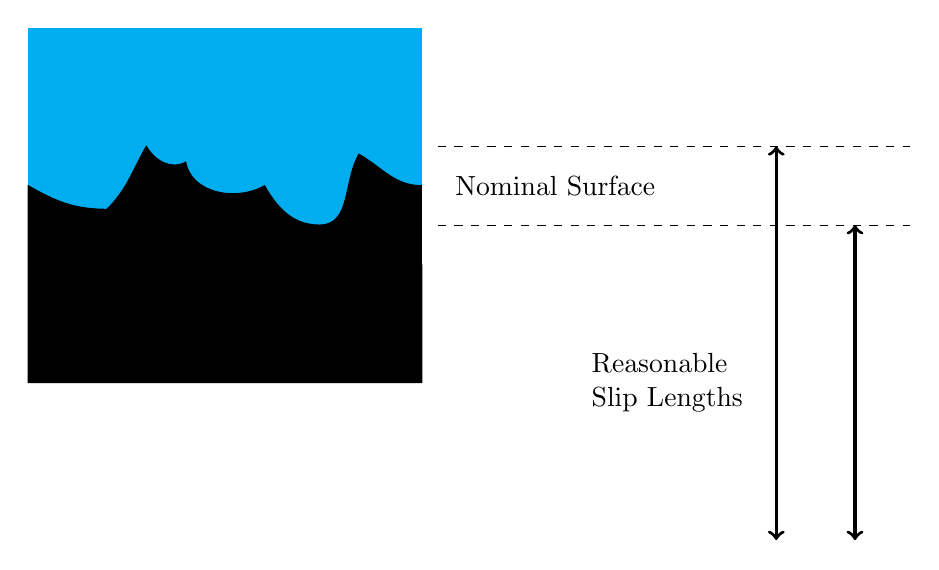
\begin{tikzpicture}
\draw[cyan, fill=cyan] (0,0) rectangle (5,3);

\filldraw (5,0) -- (5,-1.5) -- (0,-1.5) -- (0,1)  to [out=-30,in=180] 
          (1,0.7) to [out=45,in=240] (1.5,1.5)  to [out=-60,in=210] (2,1.3)
           to [out=-80,in=210] (3, 1)  to [out=-60,in=180] (3.7,0.5)
            to [out=0,in=240] (4.2,1.4)  to [out=-30,in=180] (5,1);
            
\draw[dashed] (5.2,0.5) -- +(6,0);
\draw[dashed] (5.2,1.5) -- +(6,0);

\node at (5.3,1)[right]{Nominal Surface};

\draw [<->,very thick] (9.5,1.5) -- +(0,-5);
\draw [<->,very thick] (10.5,0.5) -- +(0,-4);

\node at (9.2,-1.5) [left, align=left] {Reasonable\\ Slip Lengths};

\end{tikzpicture}
\end{center}

Surprisingly, a failure to consider the precise location of the $z=0$ point led to considerable confusion and contradiction in the early experimental literature on slip.

\vspace*{1em}

Studies were made on the effects of roughness on slip.  These involve a surface that is non-flat, but otherwise homogeneous; the material is the same everywhere, so is assumed to have the same intrinsic slip length everywhere.

\vspace*{1em}

In 2002, Zhu and Granick published results of drainage force experiments on hydrophobic surfaces of varying roughness \cite{ZhuGranick2002}.  The molecularly smooth surface showed a flow dependent slip length of up to 35 nm, while rougness \emph{suppressed} slip, with a roughness of 6 nm giving no slip at all.

They defined the $z=0$ level in the surface force appartatus by `adhesive contact in air'.  Therefore, the $z=0$ level could well be below the tops of the roughness peaks.  No effort was made to account for this.


A paper from 2003 by Bonaccurso, Butt and Craig \cite{BonaccursoButtCraig2003} claimed that roughness could \emph{increase} slip, even on a \emph{hydrophilic} (contact angle zero!) surface.
They measure drainage forces of a glass sphere approaching a silicon surface roughened up to 12.2 nm rms.

They discuss the importance of defining the zero distance.  They end up defining it at the tops of the peaks, as this is the first point of contact.  They calculate slip lengths by fitting the data to Vinogradova's model.  The best fit is when they fix the slip length on the glass sphere at about 43 nm, and increase the slip length of the substrate as roughness increases.  Under `normal' conditions, they find a slip length of 3.5 nm for maximum roughness of 12.2 nm.  But for extremely high approach velocities, for the same roughness they find a slip length of 900 nm!

Vinogradova herself waded into the issue in 2006, with a paper with Yakubov \cite{VinogradovaYakubov2006}.  They used a purpose-built AFM device that tapped a roughened sphere onto a smooth plane.  The sphere had an rms roughness of 10 -11 nm, and a maximum peak-to-valley distance of 45 nm.  With the surface taken to be at the tops of the peaks, a reduction in drainage force was observed, compared to a smooth sphere of equal diameter.  But the reduction was not due to slip:  The force was equivalent to that of a smooth sphere whose surface was located at an intermediate position between the peaks and valleys of the roughness.

Thus the issue is resolved: if the boundary is taken to be at the valleys of the roughness, then roughness reduces slip.  Conversely, if the boundary is taken to be at the tops of the peaks, then roughness \emph{increases} slip.
They note ``We believe our paper entirely clarifies the situation with flow past rough surfaces, highlights reasons for existing controversies, and resolves apparent paradoxes." 

A couple of numerical studies expand on Vinogradova's clarification.

Kunert and Harting in 2007 \cite{KunertHarting2007} formalized the concept with the introduction of an `effective no slip plane', typically located between the peaks and valleys of the surface roughness.  They carried out numerical simulations using lattice Boltzmann methods on different surfaces.  Each surface has minimum and maximum heights, $h_{\mathrm{min}}$ and $h_{\mathrm{max}}$, and an average height $h_{\mathrm{average}}$.  They calculate the position of the effective no-slip plane, $h_{\mathrm{eff}}$.  In all cases, $h_{\mathrm{eff}}$ was always considerably higher than $h_{\mathrm{average}}$.  If the surface has a few very tall but sparsely distributed spikes, then $h_{\mathrm{average}}$ can be much smaller than $h_{\mathrm{max}}$, and $h_{\mathrm{eff}}$ lies somewhere between them and cannot be well approximated by either.

In 2010 the same authors teamed up with Vinogradova \cite{KunertHartingVinogradova2010} to carry out lattice Boltzmann simulations of high-speed drainage between a smooth sphere and a randomly rough plane.  A sphere of radius $R$ approaches the plane $z=0$ located at the tops of the roughness.  Assuming that the plane $z=0$ has a single constant slip length, then asymptotically, the drainage force
\[ F \rightarrow \frac{9R}{32z} \quad \text{as} \;\;\; z \rightarrow 0 \]

Alternatively, assuming there is a no-slip plane located a distance $s$ below the top of the roughness,
\[ F \rightarrow \frac{9R}{8s} \quad \text{as} \;\;\; z \rightarrow 0 \]

At distant separations, the two models agree with each other, but at close separations, the forces predicted by the slip model are higher than observed, while the effective no-slip plane model fits the data very well.  

\vspace*{1em}

Hence, an effective no-slip plane located between the peaks and valleys of the roughness does a better job at explaining drainage forces than a slip boundary located on top of the roughness.  This is not surprising, since the drainage force of a sphere touching a surface (even with slip) will diverge, while the effective no-slip plane model always allows a finite space for fluid to escape.

However, for Couette or Poiseuille type flow, the two models should be equivalent; that is after all, one way of defining the slip length.  The important thing is to locate the effective no-slip plane.  The distance from there to the surface defined as $z=0$ determines the slip length.  These considerations are obviously still  important for any rough surface that also happens to be mixed-slip.

\begin{center}
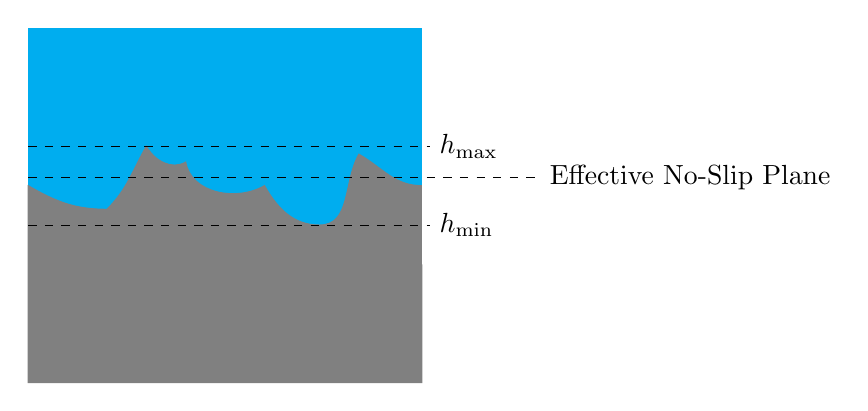
\begin{tikzpicture}

\draw[cyan, fill=cyan] (0,0) rectangle (5,3);

\filldraw [color=gray] (5,0) -- (5,-1.5) -- (0,-1.5) -- (0,1)  to [out=-30,in=180] 
          (1,0.7) to [out=45,in=240] (1.5,1.5)  to [out=-60,in=210] (2,1.3)
           to [out=-80,in=210] (3, 1)  to [out=-60,in=180] (3.7,0.5)
            to [out=0,in=240] (4.2,1.4)  to [out=-30,in=180] (5,1);
            
\draw[dashed] (0,0.5) -- +(5.1,0);
\draw[dashed] (0,1.5) -- +(5.1,0);
\node at (5.1,0.5)[right]{$h_{\mathrm{min}}$};
\node at (5.1,1.5)[right]{$h_{\mathrm{max}}$};

\draw[dashed] (0, 1.1) -- +(6.5,0);

\node at (6.5,1.1)[right]{Effective No-Slip Plane};

\end{tikzpicture}
\end{center}



\section{Mixed Slip Flow}

In 2003, Cottin-Bizonne \emph{et al} published a paper \cite{Cottin-Bizonne2003} in which they stated ``Our results show for the first time that, in contrast to common belief, surface friction may be reduced by surface roughness."  In fact, what they discovered is that flow over a rough surface may transition into the superhydrophobic state, with the fluid now flowing over vapour pockets.  (As previously stated, later that same year, Bonaccurso, Butt and Craig \cite{BonaccursoButtCraig2003} experimentally demonstrated that roughness increases slip. But they did not explicitly consider that their system may have entered the superhydrophobic regime.  Had it?)

Cottin-Bizonne and coworkers looked at molecular dynamics simulations of a Lennard-Jones fluid flowing over a flat surface decorated with narrow square posts.  At sufficiently low pressures, the fluid entered the Cassie state, as a vapour phase spontaneously formed at the surface, leaving the fluid supported on top of the posts.  The surface had an intrinsic slip length of 20 - 25 $\sigma$ (atom diameters).  In the Cassie state, slip lengths up to 57 $\sigma$ appeared.  For very narrow posts -- 4.9 $\sigma$, slip lengths could reach 130 $\sigma$.  Note that slip lengths were measured from the bottom of the cavity, so the post height --- 6 $\sigma$ --- could be added to the slip lengths.


A physical experiment of this superhydrophobic Cassie state flow was presented by Choi and Kim in 2006 \cite{ChoiKim2006}.  They were probably the first to deliberately engineer a surface for maximum slip: `nanoturf', silicon nanoposts about 1 - 2 $\mu$m high, spaced about 0.5 - 1.0 $\mu$m apart, rendered hydrophobic by a 10 - 20 nm thick layer of Teflon.  They estimated the air fraction of the surface to be 60 \%.

A commercial cone-and-plate rheometer was used to measure slip lengths: a collosal 20 $\mu$m for water and 50 $\mu$ for 30 \% glycerine solution.  (They expect this, since the viscosity of the glycerine solution is 2.5 times greater than that of water.)

Such suspiciously high slip lengths were not replicated in a more careful study by Joseph \emph{et al} also in 2006 \cite{Joseph2006}.  They did particle image velocimetry on channels coated with carbon nanotubes of diameter 50 - 100 nm, spaced 100 - 250 nm apart.  The tops of the nanotubes could be evenly spaced, or clumped together like wet hair, giving inter-clump length scales of 1.7, 3.5 or 6 $\mu$m.  The derived slip lengths for the three surface morphologies were roughly 0.4, 1.0 and 1.4 $\mu$m, respectively.

They note that their results are an order of magnitude smaller than the 20 $\mu$m slip lengths of Choi and Kim, and point out that rheological methods lack the sensitivity to measure surface effects.

An amusing effort was made by Lee and Kim in 2011 \cite{LeeKim2011} to maximize slip by making a heirarchical structured surface --- nanoposts on top of microposts.  It worked if area fraction taken up by the microposts was large enough.  Below about 10\% area fraction --- a realistic figure --- the advantage began to disappear, and at 4\% area fraction, the heirarchical surface gave \emph{lower} slip than conventional unadorned microposts.

\vspace*{1em}

A one-dimensional version of the superhydrophobic surface is a nanograting --- a surface covered with ridges, with the water supported by surface tension on top of the ridges.  In 2006, Choi \emph{et al} \cite{Choi2006} presented slip experiments on a ``well-defined nanograte": ridges 500 nm high and 50 nm wide, separated by a gap of 180 nm.  Thus the pitch (period) was 230 nm.
If the grating was left hydrophilic, they believe that water fully wets the surface, penetrating down into the troughs.  After rendering the surface hydrophobic with Teflon, they believe that there is air in the troughs.  Experiments were carried out with both states, with fluid flow both parallel to, and transverse to the ridges.

They could measure slip lengths to a resolution of only 30 nm, thus they were unsure if the hydrophobic surface had any intrinsic slip.  For flow parallel to the ridges, there was a clear distinction between the slip lengths of hydrophilic and hydrophobic surfaces.  $30 \pm 15$ nm for hydrophilic, and $143 \pm 35$ nm for hydrophobic.  For transverse flow, they found insignificant slip, $0 \pm 17$ for hydrophilic, and $61 \pm 44$ for hydrophobic.

\vspace*{1em}

One can imagine the difficulties in studying a surface of nanobubbles, given their random, uncontrolled nature.  Steinberger \emph{et al} in 2007 \cite{Steinberger2007} addressed the issue by studying flow over a flat surface covered with holes 1.3 $\mu$m wide and 3.5 $\mu$m deep.  Air can be trapped in the holes; they derive slip lengths via drainage force measurements on the resulting microbubble surface.

The plane $z=0$ is located on the flat surface, at the tops of the holes.  In the Wenzel state, with water filling the holes, they measure a slip length of $105 \pm 10$ nm.  With air trapped in the holes, bizarrely, they find a \emph{lower} slip length: a mere $20 \pm 10$ nm.  Understandably, they are puzzled by this, so they investigate.  They discover that the microbubbles protrude an estimated 200 - 400 nm above the flat surface, with the meniscus subtending an angle between $30^{\circ}$ and $60^{\circ}$ to the flat surface.  Is this protrusion into the bulk the cause of low slip lengths?

They test this hypothesis numerically, with a finite element package (Comsol).  They find a flat bubble ($\theta = 0^{\circ}$) gives maximum slip length --- about 160 nm.  Any increase in $\theta$ decreased slip, with $\theta > 45^{\circ}$ giving a lower slip length than the Wenzel state.

The following year (2008) Hyv\"{a}luoma and Harting replicate and extend Steinberger's numerics \cite{HyvaluomaHarting2008}.  By using lattice Boltzmann methods, they can model the bubble deforming under stress.  They essentially replicate Steinberger: a maximum slip of about 150 nm at zero protrusion angle, plummeting down past zero slip length for a protrusion angle greater than about $70^{\circ}$

They simulate Couette flow, so are able to investigate shear dependence.  In steady state shear-driven flow, they see a \emph{decrease} in slip length with increasing shear.  This contradicts some earlier claims.  However, higher shear rates deform the microbubbles, reducing the average height of the microbubbles.

They claim that this is consistent with Kunert and Harting 2007 \cite{KunertHarting2007}, which showed reduced slip from reduced roughness.
However a careful reading sheds doubt on this. The upshot of Kunert and Harting 2007 \cite{KunertHarting2007} is that if the peaks are lowered, then the position of the effective no-slip plane will be lowered too, but \emph{not as much.}  Thus, there is a reduced distance from the effective no-slip plane to the $z=0$ plane \emph{on the tops of the roughness peaks.} Put another way, the effective no-slip plane has actually \emph{risen} with respect to the $z=0$ plane. That is to say, the slip length has reduced (caused by reduced roughness).  


\begin{center}
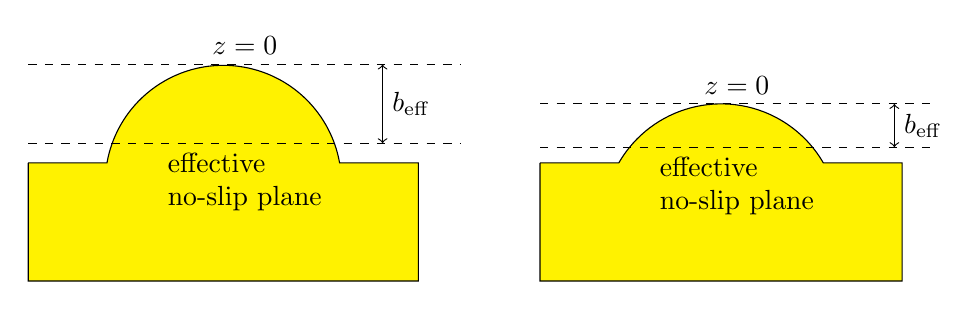
\begin{tikzpicture}

\path (0,0) coordinate (orig1);
\path (6.5,0) coordinate (orig2);

\draw[fill=yellow] (orig1) -- ++(1,0) arc(170:10:1.5) -- ++(1,0) --++(0,-1.5) -| (orig1);
\draw[dashed] (orig1) ++(0,1.25) -- node [above] {$z=0$} ++(5.5,0) ;
\draw[dashed] (orig1) ++(0,0.25) -- node [below,align=left]
{effective\\no-slip plane} ++(5.5,0);
\draw[<->] (orig1) ++(4.5,0.25) -- node[right]{\beff} ++(0,1);

\draw[fill=yellow] (orig2) -- ++(1,0) arc(150:30:1.5) -- ++(1,0) --++(0,-1.5) -| (orig2);
\draw[dashed] (orig2) ++(0,0.75) -- node [above] {$z=0$} ++(5,0) ;
\draw[dashed] (orig2) ++(0,0.2) -- node [below,align=left]
{effective\\no-slip plane} ++(5,0);
\draw[<->] (orig2) ++(4.5,0.2) -- node[right]{\beff} ++(0,0.55);

\end{tikzpicture}
\end{center}

However, in Hyv\"{a}luoma and Harting 2008 \cite{HyvaluomaHarting2008}, the $z=0$ plane is at the `top of the structured surface' which seems to mean the \emph{bottom} of the roughness.  In that case, a lowered effective no-slip plane (for any reason), is always lower with respect to the $z=0$ plane, which is equivalent to \emph{increased} slip length.  (If the effective no-slip plane was above the $z=0$ plane to start with, then the slip length becomes \emph{less negative.})

\begin{center}
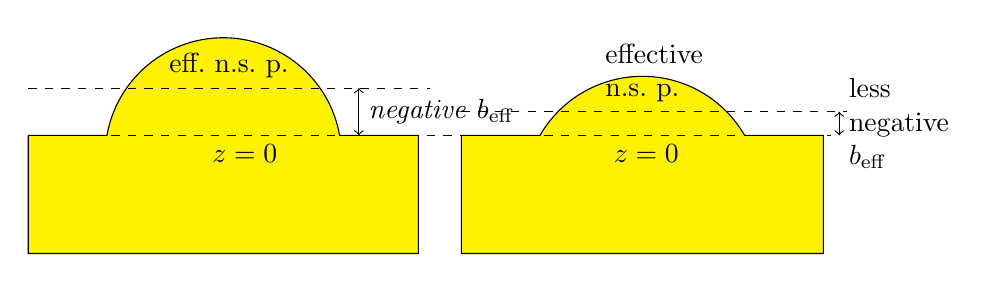
\begin{tikzpicture}

\path (0,0) coordinate (orig1);
\path (5.5,0) coordinate (orig2);

\draw[fill=yellow] (orig1) -- ++(1,0) arc(170:10:1.5) -- ++(1,0) --++(0,-1.5) -| (orig1);
\draw[dashed] (orig1) -- node [below] {$z=0$} ++(5.5,0) ;
\draw[dashed] (orig1) ++(0,0.6) -- node [above] {eff.\ n.s.\ p.} ++(5.1,0);
\draw[<->] (orig1) ++(4.2,0) -- node[right]{\emph{negative} \beff} ++(0,0.6);

\draw[fill=yellow] (orig2) -- ++(1,0) arc(150:30:1.5) -- ++(1,0) --++(0,-1.5) -| (orig2);
\draw[dashed] (orig2) -- node [below] {$z=0$} ++(4.7,0) ;
\draw[dashed] (orig2) ++(0,0.3) -- node [above,align=left]
{effective\\n.s.\ p.} ++(4.9,0);
\draw[<->] (orig2) ++(4.8,0) -- node[right,align=left]{less\\negative\\ \beff} ++(0,0.3);

\end{tikzpicture}
\end{center}

So, the increase in slip from reduced bubble height seems not to be consistent with Harting's earlier work with Kunert.  Instead, I hypothesize that a deformed bubble has a steeper wall on the downstream side, causing more stagnancy and turbulence in the lee of the bubble, thus a lower average surface velocity, hence a lower slip length.

\begin{center}
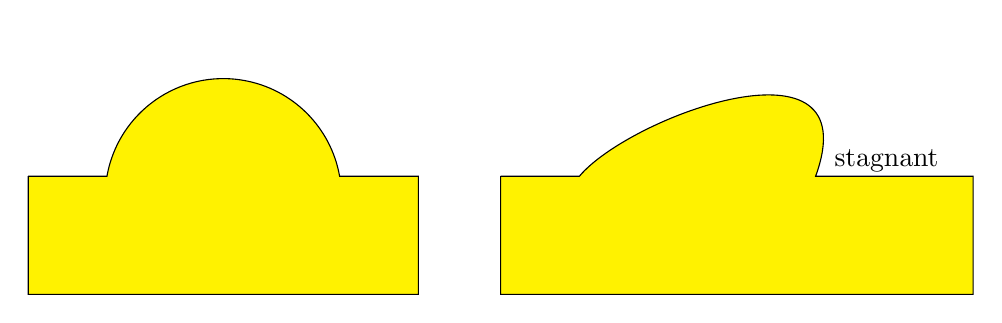
\begin{tikzpicture}

\path (0,0) coordinate (orig1);
\path (6,0) coordinate (orig2);

\draw[fill=yellow] (orig1) -- ++(1,0) arc(170:10:1.5) -- ++(1,0) --++(0,-1.5) -| (orig1);

%\draw[fill=yellow] (orig2) -- ++(1,0) to [out=60,in=180]  ++(2,1) to [out=0,in=60]
% ++(1,-1) -- ++(2,0) -- ++(0,-1.5) -| (orig2);

\draw[fill=yellow] (orig2) -- ++(1,0) .. controls +(50:1) and +(70:2) .. ++(3,0)
 -- ++(2,0) -- ++(0,-1.5) -| (orig2);

\path (orig2) ++(4.9,0.2) node {stagnant};

\end{tikzpicture}
\end{center}


Incidentally, the idea that slip is reduced by protruding bubbles had been proposed by Lauga and Brenner in 2004 \cite{LaugaBrenner2004}.  In a theoretical paper, they present a model to explain the shear-dependent slip found by Zhu and Granick in 2001 \cite{ZhuGranick2001}.  They assume that the surface was (unknown to the experimenters) covered in bubbles.  Slip lengths were inferred from the drainage force of a probe slamming into the surface at various speeds. As the probe approach velocity increases, so too does the pressure in front of it.  This increased pressure causes the bubbles to shrink, both from compression of the gas and increased diffusion into the liquid.  The reduced bubble height widens the channel, making drainage easier, for a given probe-surface distance.  Thus, this `leaking mattress effect' causes a
\nopagebreak[0] shear-dependent slip effect to appear.


\subsection*{Conclusion}

In summary, high slip lengths are possible over mixed-slip surfaces: more than 100 nanometers for nanogratings, and more than 1 micron for nanoforests.  However, the effective slip length has a slightly ambiguous definition; the quoted slip length depends on the nominal position of the $z=0$ plane.  Things are clarified by introducing the concept of an effective no-slip plane.  This is an objective concept: the surface behaves as if the no-slip plane was located at a given position.  Then, the slip length is the distance between $z=0$ and the effective no-slip plane.  Thus, if the no-slip plane becomes lower, then the slip length is increased, and vice versa.  A sensible choice for the position of the nominal $z=0$ plane is the \emph{top of the roughness.}  That way, quoted slip lengths will often be positive.  Note that if the $z=0$ plane was chosen to be \emph{below} the no-slip plane to start with, lowering the no-slip plane still \emph{increases} the slip length by making it \emph{less negative.}

%\begin{center} \vspace{3em} \Coffeecup \end{center}

\bibliography{Lund_Thesis.bib}
\bibliographystyle{plain}


\end{document}

% Put into VUW thesis format 14-02-2014

\documentclass[12pt, a4paper, twoside, openright]{book}

\usepackage{vuwthesis} % sets up some local things, mostly the front page

\setlength{\intextsep}{12pt} % set space above and below in-line float
\setlength{\abovecaptionskip}{0pt} % set space between figure and caption.

\usepackage{adjustbox}

\usepackage{amssymb, amsmath}
\usepackage{tikz}
\usetikzlibrary{calc}

\newcommand{\beff}{\ensuremath{b_{\mathrm{eff}}}}
\newcommand{\bmean}{\ensuremath{ \left< b \right> }}

\newcommand{\bmin}{\ensuremath{b_{\mathrm{min}}}}
\newcommand{\bmax}{\ensuremath{b_{\mathrm{max}}}}
\newcommand{\bhigh}{\ensuremath{b_{\mathrm{high}}}}
\newcommand{\blow}{\ensuremath{b_{\mathrm{low}}}}
\newcommand{\bslip}{\ensuremath{b_{\mathrm{slip}}}}
\newcommand{\bcu}{\ensuremath{b_{\mathrm{cu.}}}}
\newcommand{\ucu}{\ensuremath{u_{\mathrm{cu.}}}}

\newcommand{\phislip}{\ensuremath{\phi_{\mathrm{slip}}}}
\newcommand{\phisol}{\ensuremath{\phi_{\mathrm{solid}}}}
\newcommand{\sigsol}{\ensuremath{\sigma_{\mathrm{solid}}}}
\newcommand{\gamsol}{\ensuremath{ \dot{\gamma}_{\mathrm{solid}} }} 

\newcommand{\sep}{\begin{equation*} \star \end{equation*}}

%\vspace{1em}
%\colorbox[gray]{0.8}{ \textsc{Other Results} }
%\vspace{0.5em}

\newcommand{\paper}[1]
         {\colorbox[gray]{0.8}{ \textsc{#1}}
         
         }

%\usepackage{marvosym}

\usepackage{etoolbox}
\newtoggle{compilealone}
\toggletrue{compilealone}

\title{Chapter 4: Effective Slip Length Expressions: Prior Work}
\author{Nat Lund}

\begin{document}
\chapter{Effective Slip Length Expressions: Prior Work}\label{C:effslip}

This thesis presents a new expression for the effective slip length of mixed-slip surfaces.  To establish the novelty, we must place our new expression in the context of other results in this field.  Hence, this chapter is a literature review of the field of effective slip.  The results of this thesis are already published as three papers in this field \cite{HendyLund2007, LundHendy2008, Lund2012}; thus, the work of this thesis is easily placed in context amongst other peer-reviewed papers.

There are a small number of results for effective slip lengths in the literature.  In this chapter, we survey a dozen or so of them.  This cannot pretend to be comprehensive --- there may be results hidden in obscure journals, behind paywalls, or camouflaged by nonstandard terminology.  Further, mathematically equivalent results may exist in fields unrelated to fluid mechanics.  There is nothing we can do about this.  The best we can claim to do is present some `high profile' results in the field of fluid slip.


\subsection{Categorizing Results by Regime of Applicability}

The published results for an effective slip length are applicable in different physical situations.  It is useful to sort these different regimes by the following criteria:

\begin{itemize}

\item \textbf{Navier Stokes} versus \textbf{Stokes `Creeping' Flow}.  A few results use the full Navier Stokes description of fluid flow.  However, slip is very small scale phenomenon, so it is relevant only if the characteristic length scale of the flow is also very small.  In that case, the Reynolds number will be very small, and the Navier Stokes equation will be very well approximated by the simpler Stokes flow equation.  (This is covered fully in the next chapter.)  Accordingly, most results have been derived assuming only Stokes `creeping' flow.

\item \textbf{Flat} versus \textbf{Rough}. Assuming the boundary to be a plane is a major simplification, warranted on grounds of mathematical tractability.  The majority of effective slip results make this assumption.

\item \textbf{2-D Flow} (1-D Surface) versus \textbf{3-D Flow} (2-D Surface).
If the surface is symmetric in one dimension, then the flow above it will have the same symmetry.  Thus, full three-dimensional flow reduces to two-dimensional flow over a one-dimensional surface pattern.  About half of effective slip results tackle this simpler case.

\item \textbf{Perfect-slip/Zero-slip Binary Surface} or \textbf{Not.}  Assuming a binary surface, comprising regions of either vanishing slip ($b=0$), or perfect slip ($b \rightarrow \infty$) only, can enable considerable simplification of the mathematics.  Half of all effective slip results tackle this limiting case.

\end{itemize}

These categories are used to construct Table \ref{table:slipresults}.  All the papers that we shall survey in this section appear in the table, in their appropriate categories.  Some papers appear in more than one cell; in that case, the paper presents more than one result.  Note that if a paper gives a \emph{single} result for a case that \emph{subsumes} another case (eg. a 3-D result that is automatically valid for the 2-D case), then the paper appears in only \emph{one} cell.


\begin{table}
\caption{The papers (presenting effective slip lengths) surveyed in this section, 
categorized into their applicable regimes.}
\label{table:slipresults}

\vspace*{2em}
\begin{adjustbox}{center}
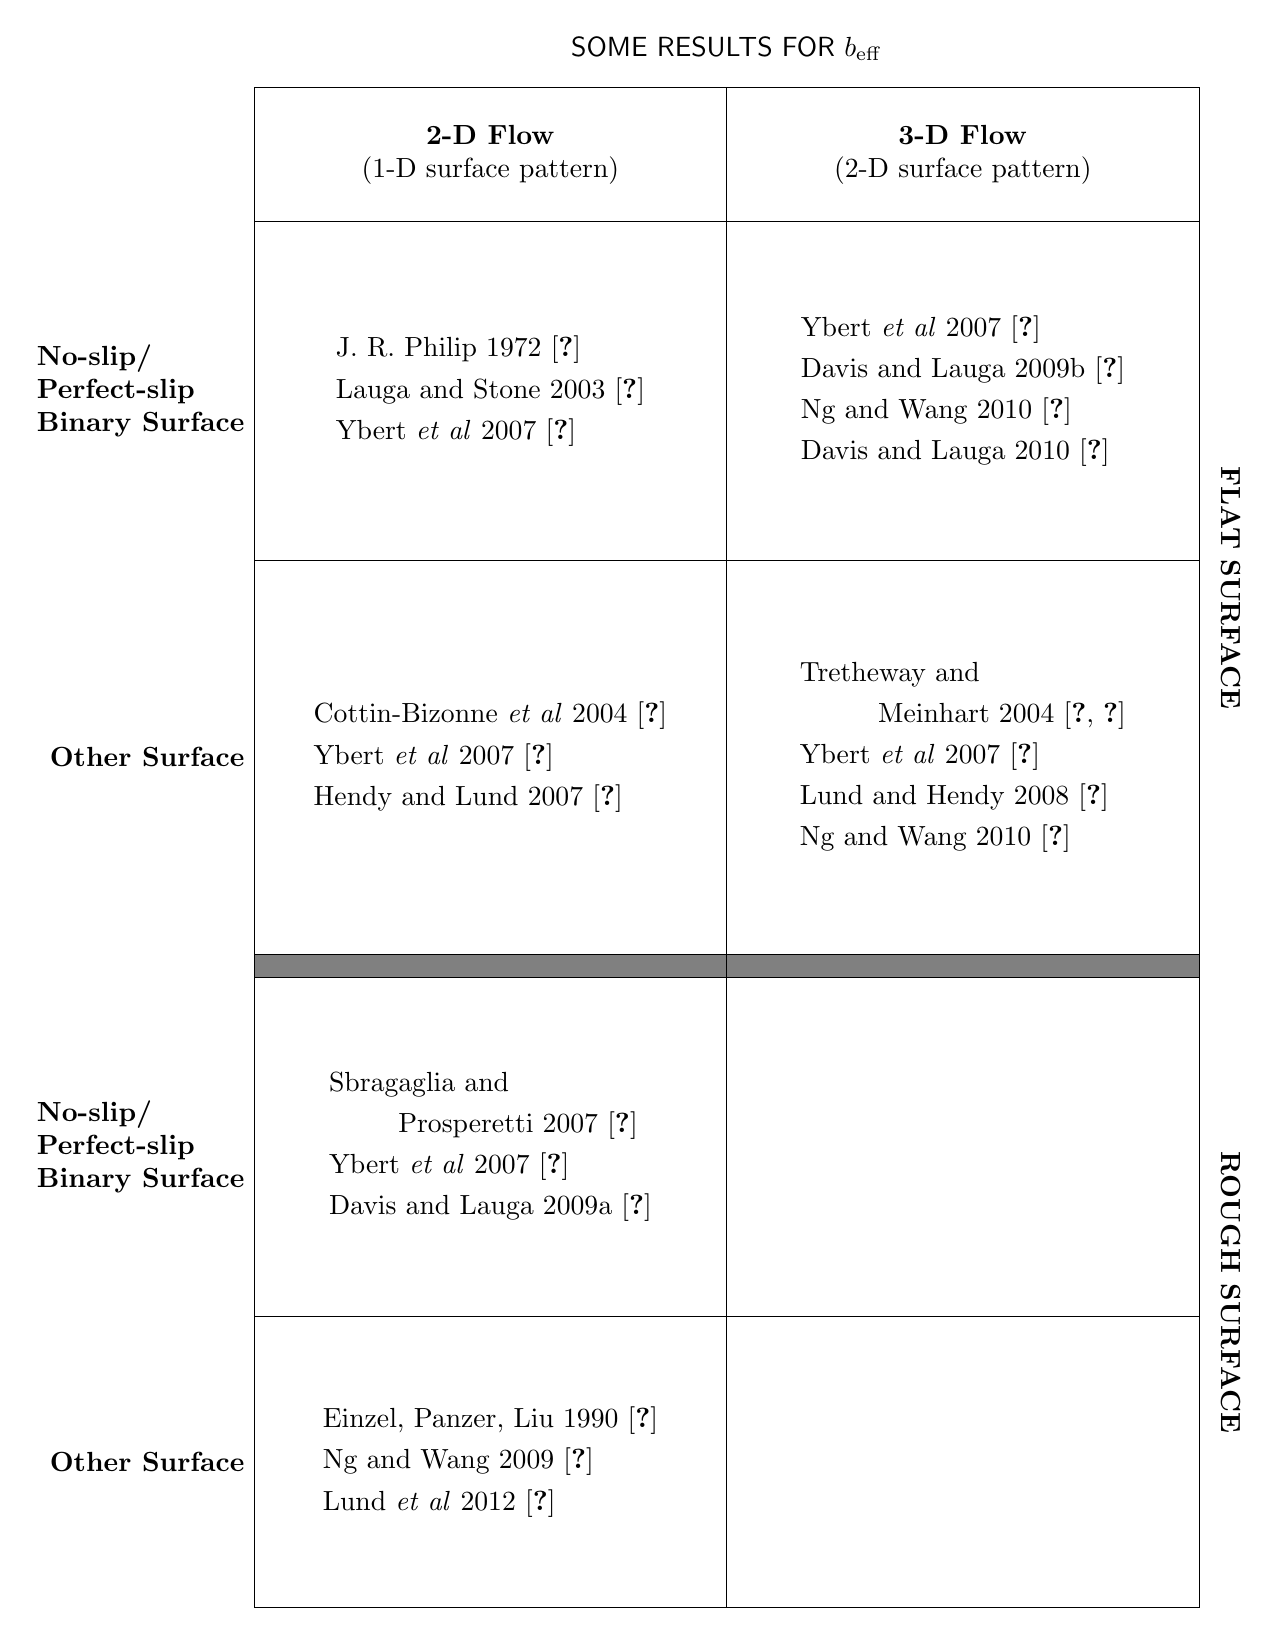
\begin{tikzpicture}

% Manually define half width of table.
\path (6,0) coordinate (midway);

% Manually define row heights.
\path (0,4.3) coordinate (flatbinary);
\path (0,5) coordinate (flatother);
\path (0,4.3) coordinate (roughbinary);
\path (0,3.7) coordinate (roughother);

\path (0,0.3) coordinate (sepwidth);

\path (0,1.7) coordinate (labelbox);

%%%%%%%%%%%%%%%%%%%%%%%%%%%%%%%%%%%%%%%%% Tikz calculates all other points...
% Bottom left corner is origin (0,0)
\path (0,0) ++(midway) coordinate (midbottom);

\path (0,0) ++(roughother) coordinate (lowdiv);
\path (lowdiv) ++(roughbinary) coordinate (belowsep);
\path (belowsep) ++(sepwidth) coordinate (abovesep);
\path (abovesep) ++(flatother) coordinate (highdiv);
\path (highdiv) ++(flatbinary) coordinate (celltop);
\path (celltop) ++ (labelbox) ++(midway) coordinate (topmid);
\path (topmid) ++(midway) coordinate (topright);


%%%%%%%%%%%%%%%%%%%%%%%%%%%%%%%%%%%%%%% Draw all boxes and lines...
\draw (0,0) rectangle (topright);
\draw (celltop) -- ++(midway) -- ++(midway);
\draw (highdiv) -- ++(midway) -- ++(midway);
\draw [fill=gray] (abovesep) ++(midway) ++(midway) rectangle (belowsep);
\draw (lowdiv) -- ++(midway) -- ++(midway);
\draw (topmid) -- (midbottom);

%%%%%%%%%%%%%%%%%%%%%%%%%%%%%%%%%%%%%%% Add flow type labels.
\path (celltop) --         coordinate[midway] (2Dlabel) (topmid);
\path (2Dlabel) ++(midway) coordinate (3Dlabel);
\node at (2Dlabel)[align=center] {\textbf{2-D Flow}\\(1-D surface pattern)};
\node at (3Dlabel)[align=center] {\textbf{3-D Flow}\\(2-D surface pattern)};

%%%%%%%%%%%%%%%%%%%%%%%%%%%%%%%%%%%%%%   Labels for surface types
\path (abovesep) -- coordinate[midway] (midflat) (celltop);
\path (0,0) --      coordinate[midway] (midrough) (belowsep);
\path (midflat) ++(midway) ++(midway) ++(0.4,0) coordinate (flatlabel);
\path (midrough) ++(midway) ++(midway) ++(0.4,0) coordinate (roughlabel);
\node at (flatlabel)  [rotate=270] {\textbf{FLAT SURFACE}};
\node at (roughlabel) [rotate=270] {\textbf{ROUGH SURFACE}};

%%%%%%%%%%%%%%%%%%%%%%%%%%%%%%%%%%%%%%%%%%%%%%%%%%%  Points in middle of rows...
\path (celltop)  -- coordinate[midway] (row1) (highdiv);
\path (highdiv)  -- coordinate[midway] (row2) (abovesep);
\path (belowsep) -- coordinate[midway] (row3) (lowdiv);
\path (lowdiv)   -- coordinate[midway] (row4) (0,0);

%%%%%%%%%%%%%%%%%%%%%%%%%%%%%%%%%%%%%%%%%%%%%%  Labels for Binary or Other surface types.

\renewcommand{\baselinestretch}{1.0}

\node at (row1) [left, align=left] {\textbf{No-slip/} \\ \textbf{Perfect-slip}\\
										\textbf{Binary Surface}};
\node at (row2) [left, align=left] {\textbf{Other Surface}};
\node at (row3) [left, align=left] {\textbf{No-slip/} \\ \textbf{Perfect-slip}\\
										\textbf{Binary Surface}};
\node at (row4) [left, align=left] {\textbf{Other Surface}};

\renewcommand{\baselinestretch}{1.24}

%%%%%%%%%%%%%%%%%%%%%%%%%%%%%%%%%%%%%%%%%%%%%%%%%  Locations of Text nodes...
%%%%%%%%%%%%  2-D Flow
\path (row1) -- coordinate[midway] (flatbin2D) +(midway);
\path (row2) -- coordinate[midway] (flatother2D) +(midway);
\path (row3) -- coordinate[midway] (roughbin2D) +(midway);
\path (row4) -- coordinate[midway] (roughother2D) +(midway);
%%%%%%%%%%%%%%  3-D Flow
\path (flatbin2D) ++(midway) coordinate (flatbin3D);
\path (flatother2D) ++(midway) coordinate (flatother3D);
\path (roughbin2D) ++(midway) coordinate (roughbin3D);
\path (roughother2D) ++(midway) coordinate (roughother3D);

%%%%%%%%%%%%%%%%%%%%%%%%%%%%%%%%%%%%%%%%%%%%%   LABEL FOR WHOLE TABLE
\path (topmid) ++(0,0.5) coordinate (heading);
\node at (heading) {\textsf{SOME RESULTS FOR \beff} };


%%%%%%%%%%%%%%%%%%%%%%%%%%%%%%%%%%%%%%%%%%%%%%%  Contents of Cells.....

\node at (flatbin2D) [align=left]
							{
							J. R. Philip 1972 \cite{Philip1972}  \\
							Lauga and Stone 2003 \cite{LaugaStone2003} \\
							Ybert \emph{et al} 2007 \cite{Ybert2007}
							};
							
\node at (flatbin3D) [align=left]
							{
							Ybert \emph{et al} 2007 \cite{Ybert2007} \\
							Davis and Lauga 2009b \cite{DavisLauga2009b} \\
							Ng and Wang 2010 \cite{NgWang2010} \\
							Davis and Lauga 2010 \cite{DavisLauga2010}
							};
							
\node at (flatother2D) [align=left]
							{
						Cottin-Bizonne \emph{et al} 2004 \cite{Cottin-Bizonne2004} \\
						Ybert \emph{et al} 2007 \cite{Ybert2007} \\
						Hendy and Lund 2007 \cite{HendyLund2007}
							};
							
\node at (flatother3D) [align=left]
							{
							Tretheway and \\
								\phantom{mmm} Meinhart 2004 \cite{TrethewayMeinhart2004,TrethewayMeinhartErratum2004} \\
							Ybert \emph{et al} 2007 \cite{Ybert2007} \\
							Lund and Hendy 2008 \cite{LundHendy2008} \\
							Ng and Wang 2010 \cite{NgWang2010}
							};
							
\node at (roughbin2D) [align=left]
							{
							Sbragaglia and \\
				\phantom{mmm}Prosperetti 2007 \cite{SbragagliaProsperetti2007} \\
							Ybert \emph{et al} 2007 \cite{Ybert2007} \\
							Davis and Lauga 2009a \cite{DavisLauga2009a}
							};

\node at (roughbin3D) [align=left]
							{
							
							};
							
\node at (roughother2D) [align=left]
							{
							Einzel, Panzer, Liu 1990 \cite{EinzelPanzerLiu1990} \\
							Ng and Wang 2009 \cite{NgWang2009} \\
							Lund \emph{et al} 2012 \cite{Lund2012}
							};

\node at (roughother3D) [align=left]
							{
							
							};
							
\end{tikzpicture}
\end{adjustbox}

\end{table}

\newpage


\subsection{Categorizing Results by Mathematical Strength}

As well as sorting the published $\beff$ results by the regime of applicability, we can sort them by the rigour of their derivation.

Mathematicians may describe a result as `exact'.  This usually means that it is in a form that can be written down as an explicit formula.  The benefit of an exact result is practical: it can be evaluated more easily.  Whether a result is exact or not is nothing to do with the rigour of its derivation; i.e. unrelated to the \emph{strength} of the result. 

In mathematics, a result is described as \emph{strong} if \emph{few assumptions} were made in its derivation.  The fewer the assumptions, the `stronger' the result.
There are two benefits of a strong result: First, because it relies on fewer assumptions, it is likely to be more widely applicable.  So `strong' means `more general'.  Secondly, the fewer assumptions, the fewer modes of failure.  Assumptions sometimes turn out to be false; this sad event may cause various results to be overturned.  A strong result is more robust.  It is less fragile to nasty surprises as the body of human knowledge grows.  (Note that a strong result may have a long complicated derivation, and thus be vulnerable to errors in the derivation.  The point is that a stronger result has a more \emph{self contained} derivation.)

\clearpage
Obviously, in theoretical physics we would like our results to be as useful and trustworthy as possible --- `exact' and `strong'.  For the purposes of this literature review, we shall rank the published results using the following (somewhat arbitrary) labels.

\begin{itemize}

\item \textbf{Derived} Results.  A relation for $\beff$ derived (mathematically) from the Stokes equation, an appropriate boundary condition, and perhaps an assumption of fluid incompressibility.

\end{itemize}

Other results:

\begin{itemize}

\item \textbf{Scaling Law} Results.  May or may not include more assumptions than a Derived Result, but the result is not exact, giving $\beff$ only as a multiple of some other length scale.

\item \textbf{Simplified} Results.  Further simplifying assumptions have been made, from reasonable phenomenological models to mere hand waving.

\item \textbf{Empirical} Results.  Exact results that express a curve fitted to either numerical or experimental data.  May be informed by stronger results.

\end{itemize}


There are comparatively fewer Derived Results.  They are listed in Table \ref{table:derivedslip}.  The other results are listed in Table \ref{table:otherslip}.


\begin{table}
%\caption{The papers surveyed here in which $\beff$ is rigorously derived from only the Stokes equation, an appropriate boundary condition and perhaps the assumption of fluid incompressibility.}
\caption{The papers surveyed here in which $\beff$ is rigorously derived from the Stokes equation and appropriate boundary conditions.}
\label{table:derivedslip}

\vspace*{2em}
\begin{adjustbox}{center}
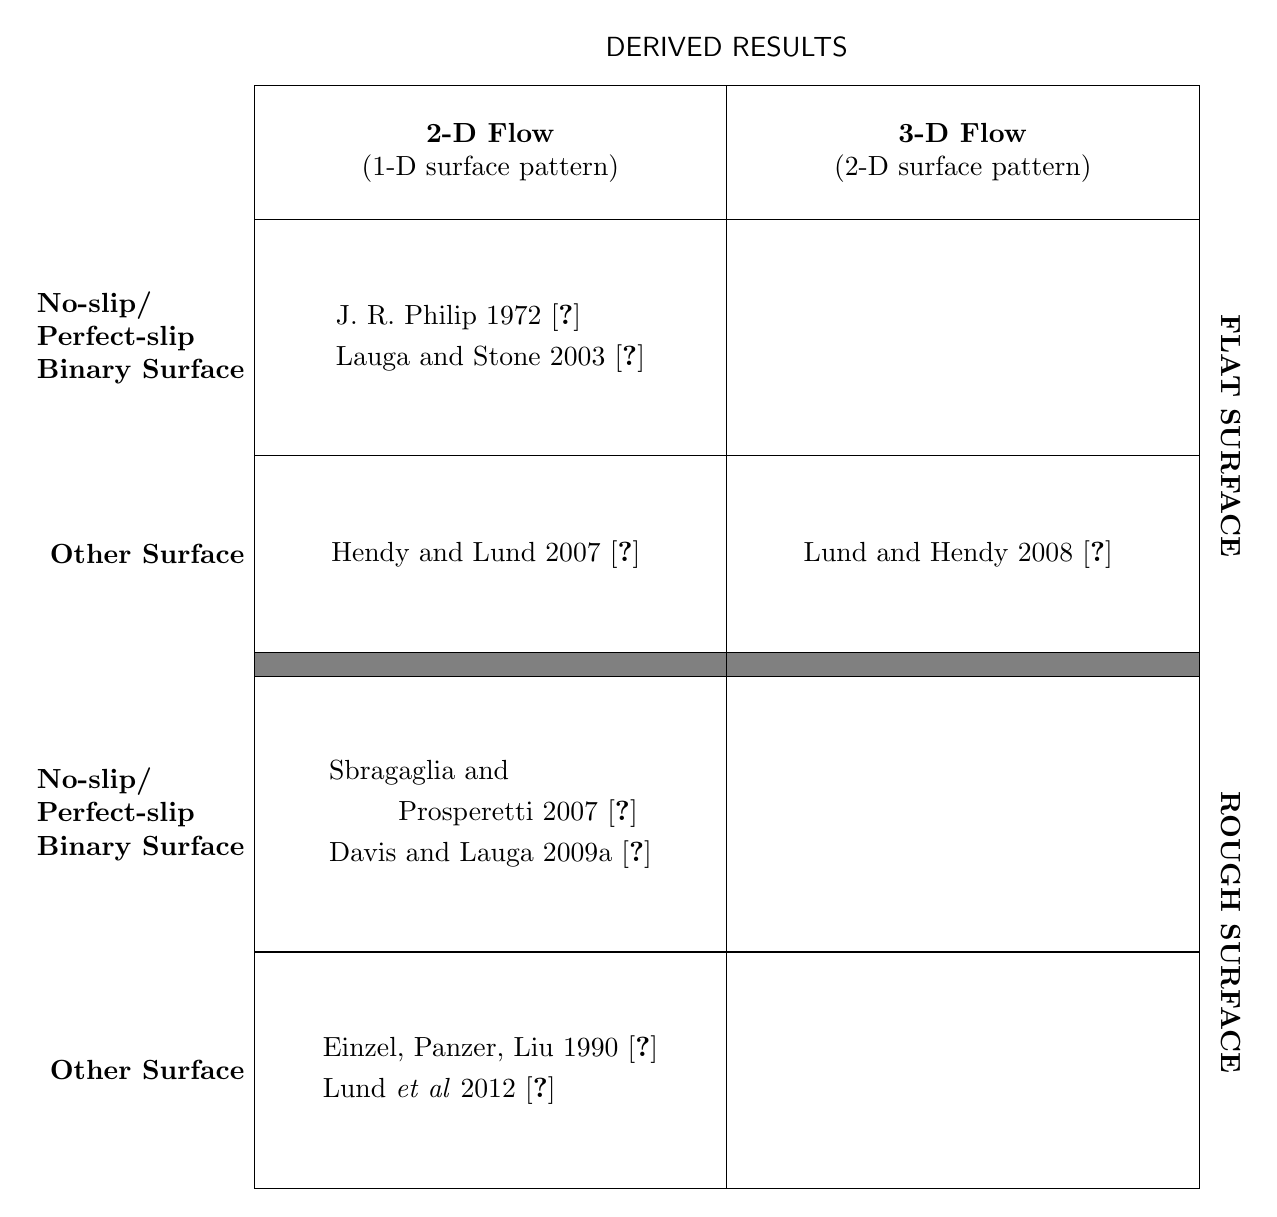
\begin{tikzpicture}

% Manually define half width of table.
\path (6,0) coordinate (midway);

% Manually define row heights.
\path (0,3) coordinate (flatbinary);
\path (0,2.5) coordinate (flatother);
\path (0,3.5) coordinate (roughbinary);
\path (0,3) coordinate (roughother);

\path (0,0.3) coordinate (sepwidth);

\path (0,1.7) coordinate (labelbox);

%%%%%%%%%%%%%%%%%%%%%%%%%%%%%%%%%%%%%%%%% Tikz calculates all other points...
% Bottom left corner is origin (0,0)
\path (0,0) ++(midway) coordinate (midbottom);

\path (0,0) ++(roughother) coordinate (lowdiv);
\path (lowdiv) ++(roughbinary) coordinate (belowsep);
\path (belowsep) ++(sepwidth) coordinate (abovesep);
\path (abovesep) ++(flatother) coordinate (highdiv);
\path (highdiv) ++(flatbinary) coordinate (celltop);
\path (celltop) ++ (labelbox) ++(midway) coordinate (topmid);
\path (topmid) ++(midway) coordinate (topright);


%%%%%%%%%%%%%%%%%%%%%%%%%%%%%%%%%%%%%%% Draw all boxes and lines...
\draw (0,0) rectangle (topright);
\draw (celltop) -- ++(midway) -- ++(midway);
\draw (highdiv) -- ++(midway) -- ++(midway);
\draw [fill=gray] (abovesep) ++(midway) ++(midway) rectangle (belowsep);
\draw (lowdiv) -- ++(midway) -- ++(midway);
\draw (topmid) -- (midbottom);

%%%%%%%%%%%%%%%%%%%%%%%%%%%%%%%%%%%%%%% Add flow type labels.
\path (celltop) --         coordinate[midway] (2Dlabel) (topmid);
\path (2Dlabel) ++(midway) coordinate (3Dlabel);
\node at (2Dlabel)[align=center] {\textbf{2-D Flow}\\(1-D surface pattern)};
\node at (3Dlabel)[align=center] {\textbf{3-D Flow}\\(2-D surface pattern)};

%%%%%%%%%%%%%%%%%%%%%%%%%%%%%%%%%%%%%%   Labels for surface types
\path (abovesep) -- coordinate[midway] (midflat) (celltop);
\path (0,0) --      coordinate[midway] (midrough) (belowsep);
\path (midflat) ++(midway) ++(midway) ++(0.4,0) coordinate (flatlabel);
\path (midrough) ++(midway) ++(midway) ++(0.4,0) coordinate (roughlabel);
\node at (flatlabel)  [rotate=270] {\textbf{FLAT SURFACE}};
\node at (roughlabel) [rotate=270] {\textbf{ROUGH SURFACE}};

%%%%%%%%%%%%%%%%%%%%%%%%%%%%%%%%%%%%%%%%%%%%%%%%%%%  Points in middle of rows...
\path (celltop)  -- coordinate[midway] (row1) (highdiv);
\path (highdiv)  -- coordinate[midway] (row2) (abovesep);
\path (belowsep) -- coordinate[midway] (row3) (lowdiv);
\path (lowdiv)   -- coordinate[midway] (row4) (0,0);

%%%%%%%%%%%%%%%%%%%%%%%%%%%%%%%%%%%%%%%%%%%%%%  Labels for Binary or Other surface types.

\renewcommand{\baselinestretch}{1.0}

\node at (row1) [left, align=left] {\textbf{No-slip/} \\ \textbf{Perfect-slip}\\
										\textbf{Binary Surface}};
\node at (row2) [left, align=left] {\textbf{Other Surface}};
\node at (row3) [left, align=left] {\textbf{No-slip/} \\ \textbf{Perfect-slip}\\
										\textbf{Binary Surface}};
\node at (row4) [left, align=left] {\textbf{Other Surface}};

\renewcommand{\baselinestretch}{1.24}

%%%%%%%%%%%%%%%%%%%%%%%%%%%%%%%%%%%%%%%%%%%%%%%%%  Locations of Text nodes...
%%%%%%%%%%%%  2-D Flow
\path (row1) -- coordinate[midway] (flatbin2D) +(midway);
\path (row2) -- coordinate[midway] (flatother2D) +(midway);
\path (row3) -- coordinate[midway] (roughbin2D) +(midway);
\path (row4) -- coordinate[midway] (roughother2D) +(midway);
%%%%%%%%%%%%%%  3-D Flow
\path (flatbin2D) ++(midway) coordinate (flatbin3D);
\path (flatother2D) ++(midway) coordinate (flatother3D);
\path (roughbin2D) ++(midway) coordinate (roughbin3D);
\path (roughother2D) ++(midway) coordinate (roughother3D);

%%%%%%%%%%%%%%%%%%%%%%%%%%%%%%%%%%%%%%%%%%%%%   LABEL FOR WHOLE TABLE
\path (topmid) ++(0,0.5) coordinate (heading);
\node at (heading) {\textsf{DERIVED RESULTS} };


%%%%%%%%%%%%%%%%%%%%%%%%%%%%%%%%%%%%%%%%%%%%%%%  Contents of Cells.....

\node at (flatbin2D) [align=left]
							{
							J. R. Philip 1972 \cite{Philip1972} \\
							Lauga and Stone 2003 \cite{LaugaStone2003}
							};
							
\node at (flatbin3D) [align=left]
							{
							};
							
\node at (flatother2D) [align=left]
							{
							Hendy and Lund 2007 \cite{HendyLund2007}
							};
							
\node at (flatother3D) [align=left]
							{
							Lund and Hendy 2008 \cite{LundHendy2008}
							};
							
\node at (roughbin2D) [align=left]
							{
							Sbragaglia and \\
					\phantom{mmm}Prosperetti 2007 \cite{SbragagliaProsperetti2007} \\
							Davis and Lauga 2009a \cite{DavisLauga2009a}
							};

\node at (roughbin3D) [align=left]
							{
							
							};
							
\node at (roughother2D) [align=left]
							{
							Einzel, Panzer, Liu 1990 \cite{EinzelPanzerLiu1990} \\
							Lund \emph{et al} 2012 \cite{Lund2012}
							};

\node at (roughother3D) [align=left]
							{
							
							};
							
\end{tikzpicture}
\end{adjustbox}

\end{table}


\begin{table}
%\caption{The papers surveyed here in which $\beff$ is not exact, or does not have a rigorous derivation.}
\caption{The papers surveyed here in which $\beff$ is \emph{not} derived from Stokes equation and boundary conditions, but instead from scaling law arguments, simplified models, curve fitting etc.}
\label{table:otherslip}

\vspace*{2em}

\begin{adjustbox}{center}
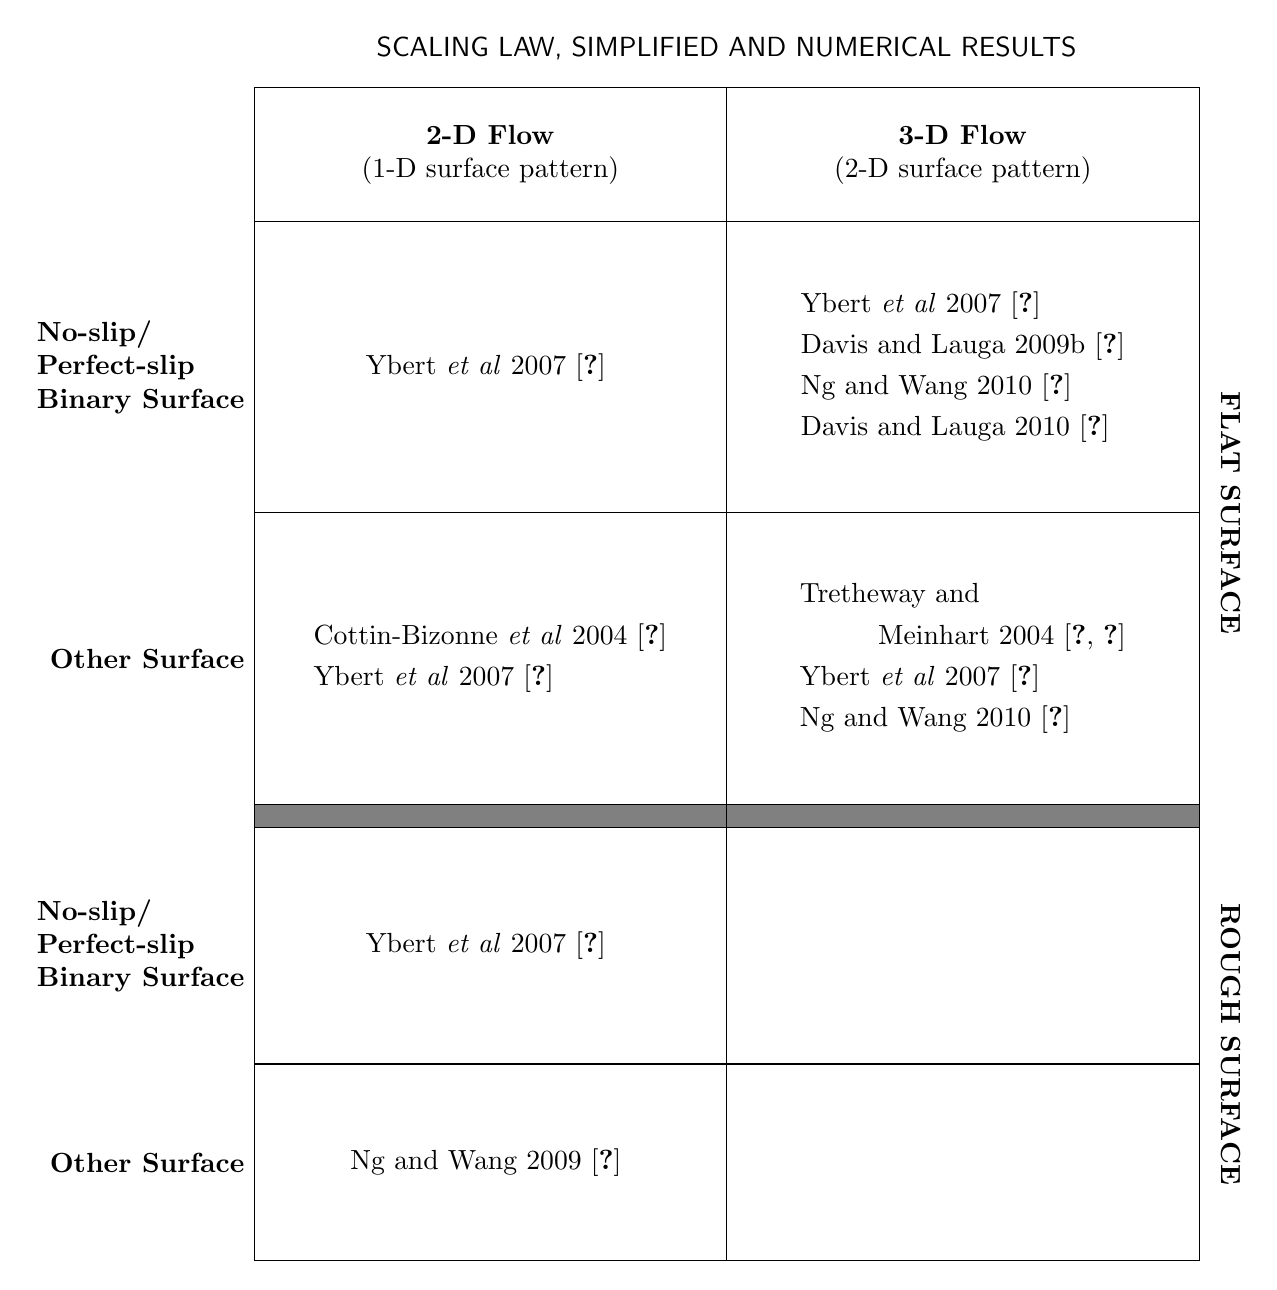
\begin{tikzpicture}

% Manually define half width of table.
\path (6,0) coordinate (midway);

% Manually define row heights.
\path (0,3.7) coordinate (flatbinary);
\path (0,3.7) coordinate (flatother);
\path (0,3) coordinate (roughbinary);
\path (0,2.5) coordinate (roughother);

\path (0,0.3) coordinate (sepwidth);

\path (0,1.7) coordinate (labelbox);

%%%%%%%%%%%%%%%%%%%%%%%%%%%%%%%%%%%%%%%%% Tikz calculates all other points...
% Bottom left corner is origin (0,0)
\path (0,0) ++(midway) coordinate (midbottom);

\path (0,0) ++(roughother) coordinate (lowdiv);
\path (lowdiv) ++(roughbinary) coordinate (belowsep);
\path (belowsep) ++(sepwidth) coordinate (abovesep);
\path (abovesep) ++(flatother) coordinate (highdiv);
\path (highdiv) ++(flatbinary) coordinate (celltop);
\path (celltop) ++ (labelbox) ++(midway) coordinate (topmid);
\path (topmid) ++(midway) coordinate (topright);


%%%%%%%%%%%%%%%%%%%%%%%%%%%%%%%%%%%%%%% Draw all boxes and lines...
\draw (0,0) rectangle (topright);
\draw (celltop) -- ++(midway) -- ++(midway);
\draw (highdiv) -- ++(midway) -- ++(midway);
\draw [fill=gray] (abovesep) ++(midway) ++(midway) rectangle (belowsep);
\draw (lowdiv) -- ++(midway) -- ++(midway);
\draw (topmid) -- (midbottom);

%%%%%%%%%%%%%%%%%%%%%%%%%%%%%%%%%%%%%%% Add flow type labels.
\path (celltop) --         coordinate[midway] (2Dlabel) (topmid);
\path (2Dlabel) ++(midway) coordinate (3Dlabel);
\node at (2Dlabel)[align=center] {\textbf{2-D Flow}\\(1-D surface pattern)};
\node at (3Dlabel)[align=center] {\textbf{3-D Flow}\\(2-D surface pattern)};

%%%%%%%%%%%%%%%%%%%%%%%%%%%%%%%%%%%%%%   Labels for surface types
\path (abovesep) -- coordinate[midway] (midflat) (celltop);
\path (0,0) --      coordinate[midway] (midrough) (belowsep);
\path (midflat) ++(midway) ++(midway) ++(0.4,0) coordinate (flatlabel);
\path (midrough) ++(midway) ++(midway) ++(0.4,0) coordinate (roughlabel);
\node at (flatlabel)  [rotate=270] {\textbf{FLAT SURFACE}};
\node at (roughlabel) [rotate=270] {\textbf{ROUGH SURFACE}};

%%%%%%%%%%%%%%%%%%%%%%%%%%%%%%%%%%%%%%%%%%%%%%%%%%%  Points in middle of rows...
\path (celltop)  -- coordinate[midway] (row1) (highdiv);
\path (highdiv)  -- coordinate[midway] (row2) (abovesep);
\path (belowsep) -- coordinate[midway] (row3) (lowdiv);
\path (lowdiv)   -- coordinate[midway] (row4) (0,0);

%%%%%%%%%%%%%%%%%%%%%%%%%%%%%%%%%%%%%%%%%%%%%%  Labels for Binary or Other surface types.

\renewcommand{\baselinestretch}{1.0}

\node at (row1) [left, align=left] {\textbf{No-slip/} \\ \textbf{Perfect-slip}\\
										\textbf{Binary Surface}};
\node at (row2) [left, align=left] {\textbf{Other Surface}};
\node at (row3) [left, align=left] {\textbf{No-slip/} \\ \textbf{Perfect-slip}\\
										\textbf{Binary Surface}};
\node at (row4) [left, align=left] {\textbf{Other Surface}};

\renewcommand{\baselinestretch}{1.24}

%%%%%%%%%%%%%%%%%%%%%%%%%%%%%%%%%%%%%%%%%%%%%%%%%  Locations of Text nodes...
%%%%%%%%%%%%  2-D Flow
\path (row1) -- coordinate[midway] (flatbin2D) +(midway);
\path (row2) -- coordinate[midway] (flatother2D) +(midway);
\path (row3) -- coordinate[midway] (roughbin2D) +(midway);
\path (row4) -- coordinate[midway] (roughother2D) +(midway);
%%%%%%%%%%%%%%  3-D Flow
\path (flatbin2D) ++(midway) coordinate (flatbin3D);
\path (flatother2D) ++(midway) coordinate (flatother3D);
\path (roughbin2D) ++(midway) coordinate (roughbin3D);
\path (roughother2D) ++(midway) coordinate (roughother3D);

%%%%%%%%%%%%%%%%%%%%%%%%%%%%%%%%%%%%%%%%%%%%%   LABEL FOR WHOLE TABLE
\path (topmid) ++(0,0.5) coordinate (heading);
\node at (heading) {\textsf{SCALING LAW, SIMPLIFIED AND NUMERICAL RESULTS} };


%%%%%%%%%%%%%%%%%%%%%%%%%%%%%%%%%%%%%%%%%%%%%%%  Contents of Cells.....

\node at (flatbin2D) [align=left]
							{
							Ybert \emph{et al} 2007 \cite{Ybert2007}
							};
							
\node at (flatbin3D) [align=left]
							{
							Ybert \emph{et al} 2007 \cite{Ybert2007} \\
							Davis and Lauga 2009b \cite{DavisLauga2009b} \\
							Ng and Wang 2010 \cite{NgWang2010} \\
							Davis and Lauga 2010 \cite{DavisLauga2010}
							};
							
\node at (flatother2D) [align=left]
							{
					Cottin-Bizonne \emph{et al} 2004 \cite{Cottin-Bizonne2004} \\
					Ybert \emph{et al} 2007 \cite{Ybert2007}
							
							};
							
\node at (flatother3D) [align=left]
							{
							Tretheway and \\
				\phantom{mmm} Meinhart 2004
				\cite{TrethewayMeinhart2004,TrethewayMeinhartErratum2004} \\
							Ybert \emph{et al} 2007 \cite{Ybert2007} \\
							Ng and Wang 2010 \cite{NgWang2010}
							};
							
\node at (roughbin2D) [align=left]
							{
							Ybert \emph{et al} 2007 \cite{Ybert2007}
							};

\node at (roughbin3D) [align=left]
							{
							
							};
							
\node at (roughother2D) [align=left]
							{
							Ng and Wang 2009 \cite{NgWang2009}
							};

\node at (roughother3D) [align=left]
							{
							};
							
\end{tikzpicture}
\end{adjustbox}

\end{table}


%\vspace{2em}

\clearpage

\section{Derived Results}

All results are for 2-dimensional flow (over a 1-dimensional surface pattern), unless otherwise noted.

\subsection{Flat Surface, of No-Slip and Perfect-Slip \\ Parallel Strips}

\paper{J.\ R.\ Philip 1972}
%The paper that arguably started it all is 
The first significant result was J.\ R.\ Philip's article in ZAMP in 1972 \cite{Philip1972}.  This comprehensive effort studied amongst other things ``Shear Flow over a Plate with a Regular Array of Longitudinal No-Shear Slots".  Note that perfect slip gives rise to the no-shear condition.  The no-shear slots are parallel to the direction of flow, as shown in Figure (\ref{JRPhilip}).   By ``generalizing the device of Karush and Young", a conformal mapping in the complex plane, he proves that in the far field:
\begin{equation}
\beff= \frac{L}{\pi}	\ln \sec \frac{\pi}{2} \phislip
\end{equation}
where $L$ is the period of the array, and $\phislip$ is the fraction of the surface that has perfect slip. Part of this proof is replicated in Appendix B. 

\begin{figure}[ht]
\centering
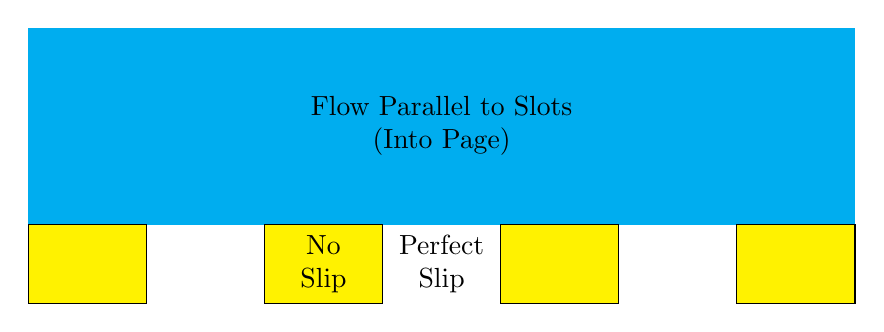
\begin{tikzpicture}
\renewcommand{\baselinestretch}{1.00}

\coordinate (slotwidth) at +(1.5,0);
\coordinate (topright) at ($7*(slotwidth) + (0,2.5)$);
\fill[cyan] (0,0) rectangle (topright);

\path (slotwidth) ++(0,-1) coordinate (box);

\foreach \n in {0,1,2,3}
    \draw[fill=yellow] ($2*\n*(slotwidth)$) rectangle +(box);

\path ($2*(slotwidth) $) -- node[align=center] {No\\ Slip} +(box);
\path ($3*(slotwidth) $) -- node[align=center] {Perfect\\ Slip} +(box);

\path (0,0) -- node[align=center] {Flow Parallel to Slots\\ (Into Page)} (topright);

\end{tikzpicture}
\caption{The no-slip/perfect-slip longitudinal flow system studied by J.~R.~Philip
in 1972.} \label{JRPhilip}
\end{figure}
%The above schematic shows the no-slip/perfect-slip longitudinal flow system studied by J.\ R.\ Philip.

\sep
\clearpage

\paper{Lauga \& Stone 2003}
It wasn't until 2003 that the case for flow \emph{transverse} to the slots was solved.  
This situation is shown in Figure (\ref{LaugaStone}).
In an article in the Journal of Fluid Mechanics that year \cite{LaugaStone2003}, Lauga and Stone study pressure-driven Stokes flow down a straight circular pipe.  They note that there is no analytic solution for the transverse case.  They derive dual series of equations, one for each boundary slip, which are simultaneously true.
%  They solve these numerically.  
With $\phislip$ fixed, the asymptotic limit of the solutions to these equations as period $L \rightarrow 0$ is the far field flow, implying an effective slip length:
\begin{equation}
\beff= \frac{1}{2} \frac{L}{\pi}	\ln \sec \frac{\pi}{2} \phislip
\end{equation}
which is exactly half the solution for parallel slots.

They provide a physical interpretation for the factor of two: ``... for a given velocity of the body in the fluid, an elongated body exerts twice as much force on the fluid when it is aligned perpendicularly to its direction of motion than when it is aligned parallel to it. As a consequence, for a given wall slip velocity ... the shear in the longitudinal case will be twice as large as the shear in the transverse case, and therefore [it is expected that] 
$b_{\mathrm{eff,} \parallel } = 2 b_{\mathrm{eff,} \perp }  $."

\begin{figure}[ht]
\centering
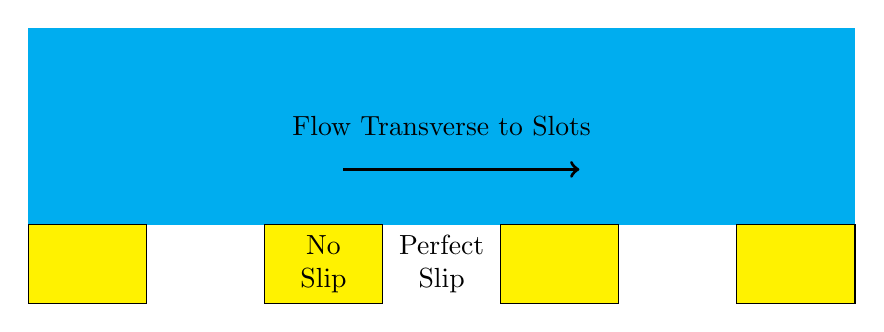
\begin{tikzpicture}
\renewcommand{\baselinestretch}{1.00}

\coordinate (slotwidth) at +(1.5,0);
\coordinate (topright) at ($7*(slotwidth) + (0,2.5)$);
\fill[cyan] (0,0) rectangle (topright);

\path (slotwidth) ++(0,-1) coordinate (box);

\foreach \n in {0,1,2,3}
    \draw[fill=yellow] ($2*\n*(slotwidth)$) rectangle +(box);

\path ($2*(slotwidth) $) -- node[align=center] {No\\ Slip} +(box);
\path ($3*(slotwidth) $) -- node[align=center] {Perfect\\ Slip} +(box);

\path (0,0) -- node[align=center] {Flow Transverse to Slots} (topright);
\draw[->,very thick] (4,0.7) -- +(3,0);

\end{tikzpicture}
\caption{The no-slip/perfect-slip transverse flow system studied by Lauga~and~Stone.} \label{LaugaStone}
\end{figure}

\clearpage
\subsection{Flat No-Slip and Curved Perfect-Slip Parallel Strips}

\paper{Sbragaglia \& Prosperetti 2007}
Philip's foundational solution had flat strips of perfect slip.  Since these model a stress-free liquid-gas interface, it is reasonable to extend the model so that the perfect slip surface forms a slightly curved meniscus, as in Figure (\ref{SbragProsp}).  In 2007, Sbragaglia and Prosperetti did exactly that \cite{SbragagliaProsperetti2007}.  Using a dual-series technique, (rather than conformal mapping), they replicate Philip's result, and add a perturbation due the the curved meniscus.  They use as a small perturbation parameter:
\begin{equation}
\epsilon = \frac{1}{2\pi} \frac{L}{2R} 
\end{equation}
where $R$ is the radius of curvature of the meniscus, and $L$ is the period of the pattern.  In the far field, the effective slip length is:
\begin{equation}
\beff= \frac{L}{\pi}	\ln \sec \frac{\pi}{2} \phislip - \frac{L^2}{4R}\phislip^3 \int_0^1 
\frac{[1-\cos(\pi\phislip s)] (1-s^2) }{\cos(\pi\phislip s) - \cos(\pi\phislip)}
\; ds
\end{equation}

They note that deformation of the meniscus \emph{reduces} the slip length. ``The physical origin of this phenomenon is due to the fact that, when the interface bows into the groove, the condition of free shear (perfect slip) is moved below the level $z=0$ of the undisturbed surface so that, on $z=0$, there is a residual nonzero stress."

\begin{figure}[ht]
\centering
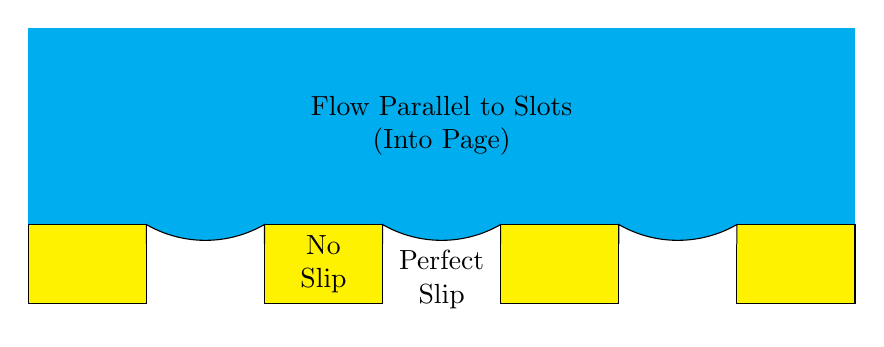
\begin{tikzpicture}

\coordinate (slotwidth) at +(1.5,0);
\coordinate (topright) at ($7*(slotwidth) + (0,2.5)$);
\fill[cyan] (0,-0.23) rectangle (topright);

\path (slotwidth) ++(0,-1) coordinate (box);

\foreach \n in {0,1,2,3}
    \draw[fill=yellow] ($2*\n*(slotwidth)$) rectangle +(box);

\foreach \n in {1,3,5}
\draw[fill=white] ($\n*(slotwidth) + (0,-0.25) $) -- ++(0,0.25) arc (240:300:1.5) -- +(0,-0.25);

\renewcommand{\baselinestretch}{1.0}

\path ($2*(slotwidth) $) -- node[align=center] {No\\ Slip} +(box);
\path ($3*(slotwidth) + (0,-0.2)$) -- node[align=center] {Perfect\\ Slip} +(box);

\path (0,0) -- node[align=center] {Flow Parallel to Slots\\ (Into Page)} (topright);

%\foreach \n in {1,3,5}
%    \draw[fill=cyan] ($\n*(slotwidth)$) arc (240:300:1.5);
    
\end{tikzpicture}
\caption{The no-slip/perfect-slip-meniscus longitudinal flow system \mbox{studied} by Sbragaglia~and~Prosperetti.} \label{SbragProsp}
\end{figure}

\sep


\paper{Davis \& Lauga 2009a}
Another variation is that the perfect-slip strips model a bubble type geometry, with the surface bulging up into the liquid.  In a 2009 paper in Physics of Fluids, Davis and Lauga consider this scenario \cite{DavisLauga2009a}.  Their model is still 2-dimensional Stokes flow, so that the `bubbles' can be considered to be the cross sections of spherical caps on top of channels full of air. Flow is thus transverse to the grating.  The channels have width $2c$, and the greater the air pressure therein, the further the bubble cap protrudes into the liquid.  The magnitude of protrusion is quantified by the angle $\theta$ that the bubble wall makes to the solid surface.
See Figure (\ref{DavisLauga}).

\begin{figure}[ht]
\centering
\begin{tikzpicture}


\coordinate (width) at (10.5,0);
\fill[cyan] (0,2.5) rectangle (width);

\coordinate (b1) at (1.5,0);
\draw[fill=white] ($(b1) + (0,-1.5)$) -- ++(0,1.5) arc (145:35:1.07) -- +(0,-1.5) coordinate (p1);
%\path (b1) -- node[above,align=center] {Perfect \\ Slip} (p1);

\coordinate (b2) at (8,0);
\draw[fill=white] ($(b2) + (0,-1.5)$) -- ++(0,1.5) arc (145:35:1.07) -- +(0,-1.5) coordinate (p2);
\draw[<->] (b2) ++(0,-1) -- node[above] {$2c$} ($(p2) +(0,0.5)$);
\draw[dashed] (b2) -- +(0.8,0) (b2) -- +(55:1 cm);
\path (b2) ++(0.5,0.19) node {$\theta$};


\draw[fill=yellow] (0,0) ++(0,-1.5) rectangle (b1);
\draw[fill=yellow] (p1) rectangle (b2);
\draw[fill=yellow] (p2) rectangle (width);

\node at (5,0) [below] {No Slip};

\path (0,0) -- node[align=center] {Flow Transverse to Slots} (topright);
\draw[->,very thick] (4,0.7) -- +(3,0);

\renewcommand{\baselinestretch}{1.0}
\node at (2.375,0.3)[below,align=center] {Perfect \\ Slip};

\end{tikzpicture}
\caption{The no-slip/perfect-slip-bubble transverse flow system studied by Davis~and~Lauga.}\label{DavisLauga}
\end{figure}

In the dilute limit, i.e. bubbles sparsely distributed on the surface, the effective slip tends to:

%\begin{multline*}
%\beff = c\pi \phislip \; \times \\
%\int_0^{\infty}
%\frac{s}{\sinh 2s(\pi -  \theta) + s \sin 2\theta}  \left[ \cos 2\theta + 
%\frac{s \sin 2\theta \cosh s \pi + \sinh s(\pi - 2 \theta)}{\sinh s \pi}
%\right] \; ds
%\end{multline*}

\begin{multline}
\beff = c\pi \phislip
\int_0^{\infty}
\frac{s}{\sinh 2s(\pi -  \theta) + s \sin 2\theta} \\
  \left[ \cos 2\theta + 
\frac{s \sin 2\theta \cosh s \pi + \sinh s(\pi - 2 \theta)}{\sinh s \pi}
\right] \; ds
\end{multline}

They evaluate for various values of $\theta$, nondimensionalized by channel width.  They find good agreement with the numerical results of Steinberger \emph{et al} \cite{Steinberger2007} and Hyv\"{a}luoma and Harting \cite{HyvaluomaHarting2008}.

``The main features of the full numerical results are seen to be reproduced by our analytical model.  There exists a critical protrusion angle $ \theta_c$ above which the effect of the wall-attached bubbles displays a transition from reduced ($ \theta < \theta_c $) to enhanced friction ($ \theta > \theta_c $).  Our model predicts $ \theta \approx 65^{\circ} $, in good agreement with the results of [Steinberger \emph{et al}] ($ \theta \approx 62^{\circ} $) and [Hyv\"{a}luoma and Harting] ($ \theta \approx 69^{\circ} $). ''

\subsection{Flat Surface, with Slip Length $\ll \gg$ Period,\\ Otherwise Arbitrary}

\paper{Hendy \& Lund 2007}
%In 2007, we published in Phys. Rev. E \cite{HendyLund2007} a perturbative proof that --- to first order --- the effective slip length is the harmonic mean of the intrinsic slip lengths
%\begin{equation}
%\beff = \left< \frac{1}{b} \right>^{-1}
%\end{equation}
%This result is valid for a flat surface with an intrinsic slip length varying in one dimension over some period $L$.  The minimum slip length must be greater than the period $L$, but may otherwise be arbitrary.


In 2007, Hendy and Lund published in Phys.\ Rev.\ E \cite{HendyLund2007} a perturbative analysis of the effective slip length of a flat surface with an intrinsic slip length $b(x)$ that varies over the surface with period $L$.  $b(x)$ has a maximum, $\bmax$, and a minimum, $\bmin$.  In the case where $ L \ll \bmin $ , the small parameter $\epsilon = L / \bmin$ expresses a perturbation of plug flow, and the effective slip length -- to first order in $\epsilon$ -- is the area-weighted harmonic mean of intrinsic slip lengths
\begin{equation}
\beff = \left< \frac{1}{b} \right>^{-1}
\end{equation}
In the opposite case, where $\bmax \ll L$, the small parameter $\epsilon = \bmax / L$ expresses a perturbation of Couette flow, and the effective slip length is found to be the area-weighted mean of intrinsic slip lengths
\begin{equation}
\beff = \left< b \right>
\end{equation}
These expressions are approximations that get better as their relevant perturbation parameters get smaller.

\vspace{1em}
\colorbox[gray]{0.8}{ \textsc{3-D Flow} }
%\vspace{0.5em} \\

\paper{Lund \& Hendy 2008}
%In 2008, we published in ANZIAM Journal \cite{LundHendy2008} an extension of the above result for 3-dimensional flow over a flat surface with a square-periodic variation in intrinsic slip length.  The perturbative proof still required that $\bmin \gg L$, with $b$ otherwise arbitrary, and the result was the same harmonic mean formula:
%\begin{equation}
%\beff = \left< \frac{1}{b} \right>^{-1}
%\end{equation}
%This published result subsumes our published result from the previous year.  It is is fully presented in Chapter 7.

In 2008, we published in ANZIAM Journal \cite{LundHendy2008} a similar perturbation analysis that extended the above results to 3-dimensional flow over a flat surface with a square-periodic variation in intrinsic slip length, $b(x,y)$.  The period in the $x$ direction is $L$. If plug flow is perturbed, with perturbation parameter $\epsilon = L / \bmin$, again the effective slip length is the area-weighted harmonic mean of $b(x,y)$:
\begin{equation}
\beff = \left< \frac{1}{b} \right>^{-1}
\end{equation}
And if Couette flow is perturbed, with small parameter $\bmax \ll L$, the effective slip length is the area-weighted mean of $b(x,y)$:
\begin{equation}
\beff = \left< b \right>
\end{equation}
These published results subsume our published results from the previous year.
They are presented in Chapter 7.


\subsection{Rough Surface, with Slip Length $ \gg$ Period,\\ Otherwise Arbitrary}

\paper{Lund \emph{et al} 2012}
Using a completely different technique --- homogenization --- we have proved that
for flow over a \emph{rough} surface with a slip length varying with the same period $L$ as the roughness, with the minimum slip length much greater than $L$,
\begin{equation}
\beff = \left< \frac{\sqrt{1 + s^2}}{b} \right>^{-1}
\end{equation}
This is the harmonic mean weighted by \emph{area of contact} between surface and fluid --- not just footprint area.  ($s$ is the slope and $\sqrt{1+s^2}$ is the arc length.)  For a flat surface, this reduces to our previous perturbative result.

This proof was published in Phys. Rev. E in 2012 \cite{Lund2012}.  It is the centrepiece of this thesis, and is presented fully in Chapter 6.


\subsection{Rough Surface of Single Intrinsic Slip}

\paper{Einzel, Panzer \& Liu 1990}  %interesting relatively early result...
Finally, there is an interesting result for a \emph{rough} surface with a \emph{single} unchanging intrinsic slip length.  In 1990 Einzel, Panzer and Liu \cite{EinzelPanzerLiu1990} studied a `weakly varying surface' of the form
\begin{equation}
y(x) = \sum_n \left[ h_n^{\cos} \cos(nkx) + h_n^{\sin} \sin(nkx) \right]
\end{equation} 
This Fourier surface has a \textbf{single} intrinsic slip length $b_0$.  In the `stick' limit, $kb_0 \ll 1$, the effective slip length is:
\begin{equation}
\beff = b_0 - \sum_n nk \left[ (h_n^{\cos})^2 + (h_n^{\sin})^2  \right]
\end{equation}
More interestingly, in the limit of perfect slip, $kb_0 \gg 1$, they get
\begin{equation}
\beff = \left[ \frac{1}{b_0} + \sum_n (nk)^3 \left[ (h_n^{\cos})^2 + (h_n^{\sin})^2 \right]
 \right]^{-1}
\end{equation}
They get a very similar result for incommensurate sine waves, so the result holds for pseudo-random roughness.

For clarity, we can apply this to simple sinusoidal surface chosen such that the wave number $k$ is the inverse of the amplitude $h$. Then the `stick' limit $k b_0 \ll 1$ is the case $b \ll L$, and
\begin{equation}
\beff = b_0 - h
 \to -h \quad \text{as} \quad b_0 \to 0
\end{equation} 
And the perfect slip limit $k b_0 \gg 1$ is the case $L \ll b$ and
\begin{equation}
\beff = \left[ \frac{1}{b_0} + \frac{1}{h} \right]^{-1}
 \to h \quad \text{as} \quad b_0 \to \infty
\end{equation}
The interesting point is that even if a rough surface has \emph{perfect slip} i.e. infinite slip length, the effective slip length of Einzel, Panzer and Liu is still finite, because of the roughness.
By contrast, our harmonic mean formula with a single slip length $b_0$ reduces to
\begin{equation}
\beff = b_0 \left< \sqrt{1 + s^2} \right>^{-1}
\to \infty \quad \text{as} \quad b_0 \to \infty
\end{equation}

\section{Simplified Models, Scaling Laws and\\ Numerics}

\subsection{Models with Simplifying Assumptions}

\paper{Tretheway \& Meinhart 2004}
In 2004, Tretheway and Meinhart \cite{TrethewayMeinhart2004} consider a variation of the binary surface wherein the gas-liquid interface has some large finite slip length, rather than an infinite slip length.  Piecing together the paper and an Erratum \cite{TrethewayMeinhartErratum2004} published 2 years later, one finds they claim that the intrinsic slip length for water of thickness $2D$ flowing over a rarefied gas layer of thickness $\delta$ is:
\begin{equation}
b_{\mathrm{slip}} = \frac{1}{2D} \left( \frac{\mu_{water}}{\mu_{air}} \right)
\left[ 2D\delta + \delta^2 + \epsilon(4D + 2\delta) \right]
\end{equation}
where $\epsilon$ is the slip length of the rarefied gas slipping over the solid.  $b_{\mathrm{slip}}$ is derived from a velocity equation $u_{\mathrm{slip}}$.  They combine this with the standard no-slip velocity equation (Couette flow):
``We combine the slip and no-slip [velocity] equations in a weighted average and calculate the cumulative velocity, $u_{\mathrm{cu.}}$, by
\begin{equation}
u_{\mathrm{cu.}} = \phi u_{\mathrm{slip}} + (1-\phi) u_{\mathrm{no-slip}}
\end{equation}
where $\phi$ is the fraction covered by gas. ..., we set the cumulative velocity at the air-water interface equal to the slip length times the shear rate at the air-water interface to obtain an equation for slip length ..."
\begin{equation}
b_{\mathrm{cu.}} = \phi \frac{1}{2D} \left( \frac{\mu_{water}}{\mu_{air}} \right)
 \left[ 2D\delta + \delta^2 + \epsilon(4D + 2\delta) \right]
\end{equation}

And that is the end of their analysis.  However, the observant reader may notice that
\begin{equation}
b_{\mathrm{cu.}} = \phi b_{\mathrm{slip}} 
\end{equation}
Perhaps due to the inconsistent notation of a derivation spread over a paper and an erratum published two years later, Tretheway and Meinhart do not mention this.
Furthermore, a careful reading seems to reveal that 
$ \partial_z u_{\mathrm{slip}} = \partial_z u_{\mathrm{no-slip}} = \dot{\gamma} $.
If the shear rate indeed does not depend on the local slip length, we can think about a binary surface with local slip lengths defined via $u_{\mathrm{slip}} = b_{\mathrm{slip}} \dot{\gamma}$ and $u_{\mathrm{low-slip}} = b_{\mathrm{low-slip}} \dot{\gamma}$.  Then one can show that a corollary of the definition of $u_{\mathrm{cu.}}$ given above is that $b_{\mathrm{cu.}} = \left< b \right>$.

Tretheway and Meinhart do not give any more explanation of cumulative velocity than the  quote above; nor of cumulative slip length.  If we interpret the cumulative slip length as a candidate for an effective slip length, then the argument in the paper would be essentially as follows: The slip length of fluid over a gas cavity, $\bslip$, is found.  Consider a binary surface with area fraction $\phi$ having slip length $\bslip$, and the remainder having $b = 0$.  Assume $\beff = \bmean$.  Then $\beff = \phi \bslip$.



%If the shear rate does not depend on the local slip length, we can think about a binary surface with more general slip conditions --- not just `no slip', with local slip lengths defined via
%$u_{\mathrm{slip}} = b_{\mathrm{slip}} \dot{\gamma}$ and $u_{\mathrm{low-slip}} = b_{\mathrm{low-slip}} \dot{\gamma}$.
%
%Then for velocities at the $z=0$ boundary:
%\begin{align}
%u_{\mathrm{cu.}} & = b_{\mathrm{cu.}} \partial_z u_{\mathrm{cu.}} \\
%u_{\mathrm{cu.}} & = b_{\mathrm{cu.}} \partial_z
%[ \phi u_{\mathrm{slip}} + (1-\phi) u_{\mathrm{low-slip}} ] \\
%u_{\mathrm{cu.}} & = b_{\mathrm{cu.}} 
%[ \phi \partial_z u_{\mathrm{slip}} + (1-\phi) \partial_z u_{\mathrm{low-slip}} ] \\
%u_{\mathrm{cu.}} & = b_{\mathrm{cu.}} [ \phi \dot{\gamma} + (1-\phi) \dot{\gamma} ]\\
%u_{\mathrm{cu.}} & = b_{\mathrm{cu.}} \dot{\gamma}\\
%\phi u_{\mathrm{slip}} + (1-\phi) u_{\mathrm{low-slip}} & = b_{\mathrm{cu.}} \dot{\gamma} \\
%\phi \frac{u_{\mathrm{slip}}}{\dot{\gamma}} + (1-\phi) \frac{ u_{\mathrm{low-slip}}} {\dot{\gamma}} & = b_{\mathrm{cu.}} \\
%\phi b_{\mathrm{slip}} + (1-\phi) b_{\mathrm{low-slip}} & = b_{\mathrm{cu.}} \\
%\left< b \right> & = b_{\mathrm{cu.}}
%\end{align}
%
%Thus, their definition of `cumulative velocity' appears to imply that $b_{\mathrm{cu.}}$ is simply the area-weighted average of local slip lengths.  If $b_{\mathrm{low-slip}} = 0$, it follows that 
%$ b_{\mathrm{cu.}} = \phi b_{\mathrm{slip}} $.

\sep

\paper{Cottin-Bizonne \emph{et al} 2004}
%A rather more convincing assumption was used in a landmark article in Eur. Phys. Journal E in 2004 by Cecile Cottin-Bizonne \emph{et al} \cite{Cottin-Bizonne2004}.

The harmonic mean formula for effective slip makes its first appearance (to the best of our knowledge) in a landmark article in Eur.\ Phys.\ Journal E in 2004 by Cecile Cottin-Bizonne \emph{et al} \cite{Cottin-Bizonne2004}.  The formula arises in the discussion of molecular dynamics (MD) simulations, which are the basis of the paper.
Cottin-Bizonne and colleagues presented MD fluid simulations in which they observed the `dewetting transition', wherein the liquid sits on top of posts, giving a large effective slip length.  They do some numerical calculations to predict the effective slip length in various regimes.  

For the regime of \textbf{No-slip/Perfect-slip} strips, they find excellent agreement with the analytic results of J.\ R.\ Philip \cite{Philip1972} and Lauga and Stone \cite{LaugaStone2003}.  Now confident in their technique, they investigate other regimes.

For strips of \textbf{No-slip and Partial-slip} material, they find that $\beff$ is fixed by the smaller of the two lengths, $b_{\mathrm{slip}}$ and the period $L$.

$\bullet$ For low slip ($b_{\mathrm{slip}} < L$), $\beff$ increases linearly, roughly $\beff = b_{\mathrm{slip}} / 4$

$\bullet$ For high slip ( $b_{\mathrm{slip}} > 10L$), $\beff$ asymptotes to a fraction of $L$. Roughly $L/10$ for flow parallel to stripes, and $L/20$ for transverse flow.

\vspace{1em}

For stripes of \textbf{Partial-slip and Perfect-slip} material, they find that $\beff$ is determined by the \emph{larger} of $b_{\mathrm{slip}}$ and period $L$.

$\bullet$ For small slip ($b_{\mathrm{slip}} \ll L$), $\beff$ is fixed by the period $L$.

$\bullet$ For high slip ($b_{\mathrm{slip}} > L$), $\beff$ increases linearly with intrinsic slip.

They advance a `simple phenomenological model' to explain this linearity:

``We introduce the interfacial friction coefficient $\lambda$, defined by ... the continuity of the tangential stress $\sigma_s$ at the solid-liquid interface:
\begin{equation}
\sigma_s = \eta \frac{\partial V}{\partial z} = \lambda V_s
\end{equation}
where $\eta$ is the viscosity of the liquid and $V_s$ [is the slip velocity]. The interfacial friction coefficient $\lambda$ is then related to the slip length $b$ by
\begin{equation}
\lambda = \frac{\eta}{b}
\end{equation}
The effective friction coefficient $\Lambda = \frac{\eta}{\beff}$ can be interpreted as the \emph{averaged friction} over the different stripes, and we obtain, accordingly, the following result for the effective macroscopic slip length as a function of the microscopic ones:
\begin{equation}
\beff = \left[ \phi \frac{1}{ b_{\mathrm{high}} }  + (1 -\phi) \frac{1}{ b_{\mathrm{low}}} \right]^{-1}
\end{equation}
which is similar to the addition rule for resistors in parallel.

In the case $b_{\mathrm{high}} \rightarrow \infty$, we expect
\begin{equation}
\beff = \frac{b_{\mathrm{low}}}{1-\phi} \;"
\end{equation}

Cottin-Bizonne \emph{et al} note ``It is important to emphasize that its validity is limited to the case where both the slip lengths, $\bhigh$ and $\blow$, are larger than the roughness periodicity $L$. Note, however, that in practice, this relationship is valid down to $\blow > 0.1L$."

To the best of our knowledge, this is the first assertion that $\beff$ is the harmonic mean of intrinsic slip lengths.  This result inspired this thesis, which provides a rigorous derivation and extension of this harmonic mean formula.

%\sep
\clearpage

\paper{Ng \& Wang 2009}
In 2009, Ng and Wang \cite{NgWang2009} considered flow over the familiar binary surface of flat perfect-slip/partial-slip regions, with one difference: the perfect-slip gas-liquid interface was allowed to be some distance $d$ below the solid surface.  They did numerical evaluations of flow both parallel and transverse to the resulting `step function profile' surface.
They compare their numerics with the continuum modeling results of Cottin-Bizonne \emph{et al.}\ 2004 \cite{Cottin-Bizonne2004}, and find essentially perfect agreement.

However, their most interesting observation relates to the conventional completely flat binary surface.  They recall Cottin-Bizonne's proposal for $\beff$ for flow parallel to the strips:
\begin{equation}
\beff = \frac{b_{\mathrm{solid}}}{1 - \phi}
\end{equation}
which works very well for large $b_{\mathrm{solid}}$.  Ng and Wang have discovered that this is much improved by simply adding on J.\ Philip's exact result \cite{Philip1972} for $b_{\mathrm{solid}}=0$:
\begin{equation}
\beff =  \frac{L}{\pi} \ln \left[ \sec \left( \frac{\pi}{2} \phi \right) \right] +
 \frac{b_{\mathrm{solid}}}{1 - \phi}
\end{equation}

And similarly, for transverse flow, add on the exact solution of Lauga and Stone \cite{LaugaStone2003}
\begin{equation}
\beff = \frac{1}{2}  \frac{L}{\pi} \ln \left[ \sec \left( \frac{\pi}{2} \phi \right) \right] +
 \frac{b_{\mathrm{solid}}}{1 - \phi}
\end{equation}

Ng and Wang test these extended formulae numerically, and find that they give a maximum error of 3\% -- 6\%, compared with Cottin-Bizonne's original formula which can have a maximum error of more than 50\% for small $b_{\mathrm{solid}}$.

\clearpage
\subsection{The Scaling Laws of Ybert \emph{et al}}

\paper{Ybert \emph{et al} 2007}
Possibly the highest-profile article relating to effective slip length is the 2007 article in Physics of Fluids by Ybert and coworkers, entitled ``Achieving large slip with superhydrophobic surfaces: Scaling laws for generic geometries" \cite{Ybert2007}. The authors form a research group at Lyon, France, which includes Cecile Cottin-Bizonne.  Hence, the paper makes the same assumptions as the `phenomenological model' of Cottin-Bizonne 2004 \cite{Cottin-Bizonne2004}, and takes them in a slightly different direction, to get scaling laws for various geometries.
The paper is sufficiently influential, and the derivation sufficiently instructive, that we essentially reproduce it here.

At the heart of the model is the concept of stress balance.  Consider the stress on a plane of infinitesimal area located on the fluid boundary.  The stresses are illustrated in Figure (\ref{stressbalance}).

%\clearpage

\begin{figure}[ht]
\centering
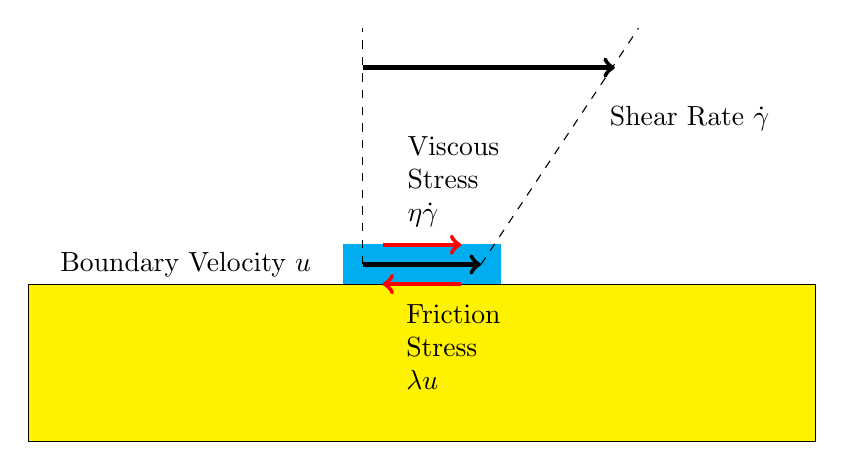
\begin{tikzpicture}

\filldraw[color=cyan] (0,0) rectangle (2,0.5);
\draw [fill=yellow] (-4,0) rectangle (6,-2);

\coordinate (ref) at (0.25,0.25);
\draw[->,ultra thick] (ref) -- ++(1.5,0);
\draw[dashed] (ref) -- ++(0,3);
\draw[->, ultra thick] (ref) ++(0,2.5) -- ++(3.2,0);
\draw[dashed] (ref) ++(1.5,0) -- ++(2,3);

\node at (-2,0.25) {Boundary Velocity $u$};
\node at (4.4,2.1) {Shear Rate $\dot{\gamma}$};

%%%%%%%%%%%%%%  Stress arrows
\draw [<-, ultra thick, color=red] (0.5,0) -- ++(1,0);
\draw [->, ultra thick, color=red] (0.5,0.5) -- ++(1,0);

\renewcommand{\baselinestretch}{1.0}

\node at (1.4,1.3) [align=left] {Viscous\\ Stress\\ $\eta \dot{\gamma} $};
\node at (1.4,-0.8) [align=left] {Friction\\Stress\\ $\lambda u$};

\end{tikzpicture}
\caption{The balanced stresses on a fluid element at the boundary.} \label{stressbalance}
\end{figure}


At equilibrium, the stresses balance:
\begin{equation}
\sigma = \eta \dot{\gamma} = \lambda u
\end{equation}
If the stress balance is assumed to always hold locally -- at any infinitesimal plane, then the \emph{average} stresses over the entire surface (or over one period) must balance:
%The stress can be \emph{averaged} over the entire surface (or over one period):
\begin{equation}
\left< \sigma \right> = \left< \eta \dot{\gamma} \right> = \left< \lambda u \right>
\end{equation}
Now the viscosity $\eta$ can be considered constant throughout the fluid, so that $  \left< \eta \dot{\gamma} \right> = \eta \left< \dot{\gamma} \right> $.  But the friction coefficient $\lambda$ is not constant.  Therefore, Ybert \emph{et al} define an effective friction coefficient such that:
\begin{equation}
\left< \lambda u \right> = \lambda_{\mathrm{eff}} \left< u \right>
\end{equation}
\begin{equation}
\text{But then of course} \quad
\eta \left< \dot{\gamma} \right> = \lambda_{\mathrm{eff}} \left< u \right>
\quad \text{rearranges to}  \quad
\left< u \right> = \frac{\eta}{ \lambda_{\mathrm{eff}} } \left< \dot{\gamma} \right> 
\end{equation}
which defines some kind of effective slip length:
\begin{equation}
\beff = \frac{\eta}{ \lambda_{\mathrm{eff}} }  
\end{equation}
This definition of $\beff$ relates the \emph{area average} boundary velocity to the \emph{area average} of the shear rate at the boundary.
\begin{equation}
\left< u \right> = \beff \left< \dot{\gamma} \right> 
\end{equation}
Note that the variations in boundary velocity and shear rate decay with height, so that sufficiently far above the surface there is a uniform velocity and shear rate, from which our far-field effective slip length can be inferred.   If the decay process (due to momentum diffusion) is equivalent to the simple averaging done here, then the $\beff$ of Ybert \emph{et al} will be identical to our preferred far-field definition of $\beff$.  But we cannot assume this.

\vspace*{1em}
\colorbox[gray]{0.8}{ \textsc{2-D Flow over Perfect-slip/No-slip Surface} }
\vspace{0.5em}

It is assumed that the average stress on a binary surface can be decomposed into the area-weighted averages of the `subaverages' of stress over the liquid-gas interface and the liquid-solid interface:

Then 
\begin{equation}
\left< \sigma \right> = \phi \left< \sigma_{\mathrm{gas}} \right> + 
\phisol \left<  \sigsol \right> 
\end{equation}
If the gas-liquid interface is considered to be perfect-slip or \emph{no-shear}, there is no stress; $ \sigma_{\mathrm{gas}} = 0 $.  Hence 
\begin{equation}
\left< \sigma \right> = \phisol \left<  \sigsol \right>
\end{equation}
\begin{equation}
\text{Viscosity $\eta$ is constant, so} \;\;\;
\left< \sigsol \right> = \eta \left< \dot{\gamma}_{\mathrm{solid}} \right>
\end{equation}
\begin{equation}
\text{For flow over a flat surface, `simple shear' obtains:} \quad
\dot{\gamma}_{\mathrm{solid}} = \frac{\partial u}{\partial z}
\end{equation}

So
\begin{equation}
\left< \sigsol \right> = \eta \left< \frac{\partial u}{\partial z} \right>
\end{equation}

\vspace{1em}
\colorbox[gray]{0.8}{ \textsc{Case where $\phisol \rightarrow 0$, Mostly Plug-like flow.} }
\vspace{0.5em}

The flow is mostly plug-like, with some characteristic velocity $U$.  The only place that it is not plug-like is in the vicinity of the post.  The fluid sticks to the top of the post (no-slip), perturbing the plug-like flow.  The perturbed region extends some (arbitrary) distance $d$ above the post, at which point the velocity is (arbitrarily) close to $U$ again.  This is shown in the diagram of Figure (\ref{plugnpost}).

%\clearpage

\begin{figure}[ht]
\centering
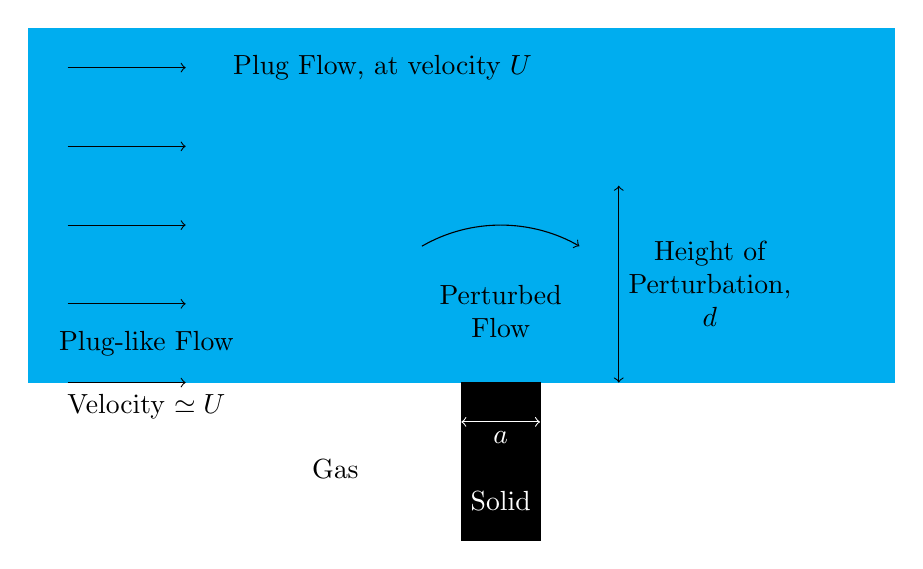
\begin{tikzpicture}

\filldraw[color=cyan] (-5.5,0) rectangle (5.5,4.5);
\filldraw (0,0) rectangle (1,-2);

\node at (-1.6,-1.1) {Gas};

\draw[<->,color=white] (0,-0.5) -- node [below] {$a$} ++(1,0);
\node at (0.5,-1.5) [color=white] {Solid};

\draw (0.5,2) arc (90:120:2cm);
\draw[->] (0.5,2) arc (90:60: 2cm);

\foreach \z in {0,1,2,3,4}
     { \draw[->] (-5,\z) -- ++(1.5,0);
      % \draw[->] (4,\z) -- ++(1,0);
      }

\draw[<->] (2,0) -- ++(0,2.5);

\renewcommand{\baselinestretch}{1.0}       
\node at (0.5,0.9) [align=center] {Perturbed\\Flow};
\node at (2,1.25) [right, align=center]{Height of \\Perturbation,\\ $d$};

\node at (-4,0.5) {Plug-like Flow};
\node at (-4,-0.3) {Velocity $\simeq U$};
%\node at (4,0.5)  {Plug-like Flow};
\node at (-1,4) {Plug Flow, at velocity $U$};
       
\end{tikzpicture}
\caption{Plug flow perturbed by a no-slip post of width $a$.}\label{plugnpost}
\end{figure}



\begin{figure}[ht]
\centering
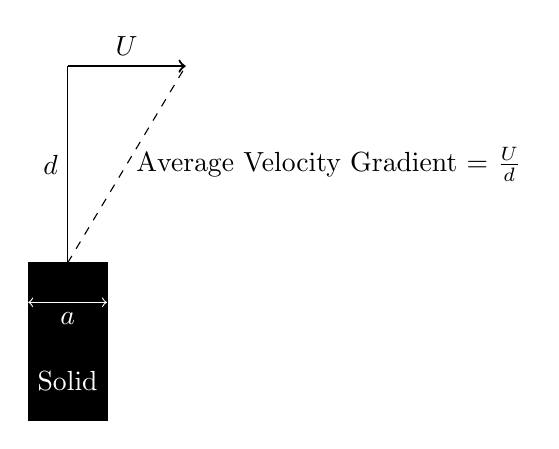
\begin{tikzpicture}

\filldraw (-0.5,0) rectangle ++(1,-2);
\draw[<->,color=white] (-0.5,-0.5) -- node [below] {$a$} ++(1,0);
\node at (0,-1.5) [color=white] {Solid};

\draw (0,0) -- node [left] {$d$} +(0,2.5);
\draw [->,thick] (0,2.5) -- node[above] {$U$} +(1.5,0);
\draw [dashed] (0,0) -- node[right] {Average Velocity Gradient = $\frac{U}{d}$} (1.5,2.5);

\end{tikzpicture}
\caption{The geometry of the average velocity gradient of the perturbation.}
\label{perturbationgeometry}
\end{figure}

Thus, the velocity changes from 0 to $U$ in distance $d$. The geometry in Figure (\ref{perturbationgeometry}) illustrates that the average velocity gradient is therefore
\begin{equation}
\left< \frac{\partial u}{\partial z} \right> = \frac{U}{d}
\end{equation}
Now, $d$ scales as $a$.  This is shown by dimensional analysis using the Buckingham Pi theorem in Appendix C.

Hence,
\begin{equation}
\left< \frac{\partial u}{\partial z} \right> \sim \frac{U}{a}
\end{equation}
%Ybert and company justify the foregoing succintly: ``To estimate $ \left< \gamsol \right> $, we recall that the Stokes equation has a Laplacian form, which strongly couples the spatial dependence of the velocity profile along the different axes ($x,y,z$). This implies that $ \left< \gamsol \right> = \left< \partial u / \partial z \right> \sim U/a $, with $a$ the typical size of the solid area."
Thus, 
\begin{equation}
\left< \sigsol \right> \sim \eta \frac{U}{a}
\end{equation}
and
\begin{equation}
\left< \sigma \right> \sim \phisol \eta \frac{U}{a}
\end{equation}
%The other interesting thing about mostly
In plug-like flow most of the fluid at the boundary is moving at the characteristic velocity $U$. So
\begin{equation}
\left< u \right> \simeq U
\end{equation}
Thus we have
\begin{equation}
\eta \left< \dot{\gamma} \right> = \left< \sigma \right> \sim
  \frac{ \phisol \eta} {a} \left< u \right>
\end{equation}
simplifying to:
\begin{equation}
\left< u \right> \sim \frac{a}{\phisol}  \left< \dot{\gamma} \right>
\end{equation}
defining
\begin{equation}
\beff \sim  \frac{a}{\phisol} 
\end{equation}
Thus in the limit of small solid fraction $\phisol$, Ybert \emph{et al} argue that
\begin{equation}
\beff \sim \alpha  \frac{a}{\phisol} 
\end{equation}
where $\alpha$ is a prefactor that depends on the geometry of the surface.  This is the main result of Ybert \emph{et al} 2007 \cite{Ybert2007}.

%\clearpage

\vspace{1em}
\colorbox[gray]{0.8}{ \textsc{Other Results} }
\vspace{0.5em}


Ybert \emph{et al} compare this scaling law with the exact result of J.\ R.\ Philip \cite{Philip1972}.  For the striped surface in question, $\phisol = a/L$, so the scaling law is:
\begin{equation}
\beff \sim L
\end{equation}
They note that in the limit of small $\phisol$, Philip's exact solution is similar, having only logarithmic dependence on $\phisol$: $\beff \sim L \log \phisol $


\vspace{1em}

If the surface is a forest of nanopillars, $\phisol = (a/L)^2$, so the scaling law is:
\begin{equation}
\beff \sim  \frac{a}{\sqrt{ \phisol}} 
\end{equation}

\vspace{1em}
Finally, if the no-slip condition is relaxed and some finite slip length $b_s$ holds on the solid post, the scaling law is modified:
``Going back to the above derivation ... in the limit $\phisol \to 0$, one expects that a finite slip length on the solid will reduce the shear rate over the solid regions: $ \left< \partial u / \partial z \right> \sim U/(a+b_s)  $. The averaged shear stress over the total surface now reads $\left< \sigma \right> = \phisol \eta U / ( a + b_s)$. One gets accordingly ..."
\begin{equation}
\beff \sim  \frac{a + b_s}{\phisol} 
\end{equation}

\vspace{1em}
For completeness, they consider the case of vanishing gas area.  Flow over a surface with very narrow gas gaps of width $l$ will be close to Couette flow, with:
\begin{equation}
\beff \sim l (1-\phisol) 
\end{equation}

%The paper also features a few more formulae of a more speculative nature, which we won't mention here.


\clearpage
\subsection{Numerics}

\paper{Ng \& Wang 2009}
As already mentioned, Ng and Wang in 2009 \cite{NgWang2009} did numerical studies of flow over a grating, in both parallel and transverse orientations. They derive eigenfunction expansions of the flow solutions, which are solved numerically.  The effective slip lengths extracted have essentially perfect agreement with the continuum modeling of Cottin-Bizonne 2004 \cite{Cottin-Bizonne2004}.

\sep

\paper{Davis \& Lauga 2009b}
In their second paper of 2009 \cite{DavisLauga2009b}, Davis and Lauga consider Stokes flow over a mesh of thin wires or strips, with large square air gaps in between.  The surface is considered to be flat, with no-slip on the strips, and perfect-slip on the liquid-air interface.  The period of the square-periodic mesh is $L$, and the width of the strips is $\epsilon L$.  See Figure (\ref{mesh}).

\begin{figure}[ht]
\centering
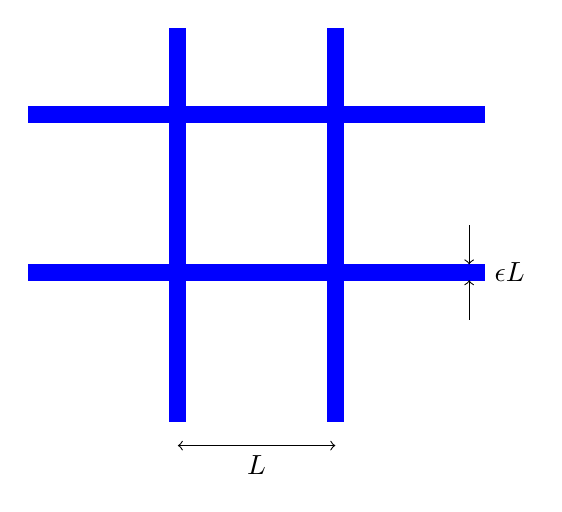
\begin{tikzpicture}

\filldraw[color=blue] (0,0) rectangle +(0.2,5);
\filldraw[color=blue] (2,0) rectangle +(0.2,5);
\draw[<->] (0.1,-0.3) -- node[below]{$L$} +(2,0);

\filldraw[color=blue] (-1.8,2) rectangle +(5.8,-0.2);
\filldraw[color=blue] (-1.8,4) rectangle +(5.8,-0.2);
\draw[<-] (3.8,2) -- +(0,0.5);
\draw[<-] (3.8,1.8) -- +(0,-0.5);
\node at (4,1.9)[right] {$\epsilon L$};

\end{tikzpicture}
\caption{Top view of the mesh of no-slip strips and perfect-slip squares.}
\label{mesh}
\end{figure}

Davis and Lauga use a method of superposition of singularities, and end up with an infinite system of linear equations.  Then $\beff = L/\pi (A_0 + B_0)$ where $A_0$ and $B_0$ are the zeroth-order coefficients of the system of equations.

They solve numerically for $A_0$ and $B_0$ by truncating the infinite system at $N$ equations.  (Truncating at $N=1000$ rather than $N=100$ changed the computed $\beff$ by less than $0.01\%$.) After computing $\beff$ for various values of $\epsilon$, they derive a least-squares fit formula:
\begin{equation}
\beff = -0.107 L \ln \phisol + 0.003L
\end{equation}

Finally, they offer `simple estimates' -- solutions from truncating the infinite series at $N=1$ and $N=2$ terms. For $N=1$:
\begin{equation}
\beff = \frac{L}{3\pi} \ln \left( \frac{2}{\pi \epsilon} \right)
\end{equation}

The simple estimate for $N=2$ is more complicated.  These simple estimates overestimate $\beff$ by up to 10\%, but converge on the correct result as $\epsilon \rightarrow 0$.

\subsection{Coefficients Evaluated for Ybert's Scaling Laws}

The influential scaling law paper by Ybert \emph{et al} \cite{Ybert2007} inspired researchers to find the relevant coefficients by numerical or approximate methods.

\paper{Ng \& Wang 2010}
In 2010, Ng and Wang \cite{NgWang2010} continued their approach of numerically solving eigenfunction expansions, to find the scaling coefficients.

For flow over superhydrophobic surfaces, with the solid posts occupying a small area fraction, Ybert had proposed:
\begin{equation}
\beff \sim \frac{1}{\sqrt{\phisol}}
\end{equation}
From their numerical data, Ng and Wang fit the parameters:
\begin{align}
\beff &= \frac{0.34}{\sqrt{\phisol}} - 0.468 \quad \text{for circular posts,} \\
\beff &= \frac{0.33}{\sqrt{\phisol}} - 0.461 \quad \text{for square posts.}
\end{align}

And other parameters for other regimes.  Ng and Wang present numerically fitted parameters for the nanobubble case ($\phisol \rightarrow 1$), for cases with finite slip on the solid, and for cases where the geometry is elliptical or rectangular rather than simply circular or square.

\sep

\paper{Davis \& Lauga 2010}
In 2010, Davis and Lauga \cite{DavisLauga2010} studied Stokes flow over a superhydrophobic surface comprising a rectangular array of circular posts, each of radius $a$, as in the diagram of Figure (\ref{posts}).

\begin{figure}[ht]
\centering
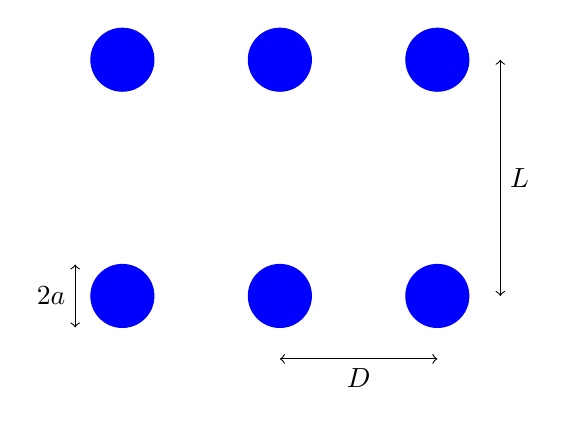
\begin{tikzpicture}

\filldraw[color=blue] (0,0) circle (4mm);
\filldraw[color=blue] (2,0) circle (4mm);
\filldraw[color=blue] (4,0) circle (4mm);
\filldraw[color=blue] (0,3) circle (4mm);
\filldraw[color=blue] (2,3) circle (4mm);
\filldraw[color=blue] (4,3) circle (4mm);

\draw[<->] (-0.6,-0.4) -- node[left]{$2a$} +(0,0.8);
\draw[<->] (2,-0.8) -- node[below]{$D$} +(2,0);
\draw[<->] (4.8,0) -- node[right]{$L$} +(0,3);

\end{tikzpicture}
\caption{Top view of rectangular array of circular posts.}\label{posts}
\end{figure}

As their point of departure, they take the scaling law proposed in Ybert \emph{et al} 2007 for the limit of small $\phisol$:
\begin{equation}
\beff \sim \frac{A}{\sqrt{\phisol}} L - BL  \label{eq:DavisLauga}
\end{equation}

%They attack the problem with Fourier transform techniques, and end up with an infinite system of linear equations for coefficients.  They make an `asymptotic estimate' of the coefficients, and get:
``By asymptotically considering the case of low solid fraction, $\phisol$, we mathematically derive the scaling coefficients $A$ and $B$ governing (\ref{eq:DavisLauga}),  thereby predicting analytically the effective surface-slip length."
The asymptotic estimate of the coefficients yields:
\begin{equation}
\beff \sim \frac{3}{16} \sqrt{ \frac{\pi}{\phisol}} \sqrt{DL}
\end{equation}
If the array is square, this reduces to:
\begin{equation}
\beff \sim \frac{3}{16} \sqrt{ \frac{\pi}{\phisol}} L
\end{equation}
Adding the next-order correction term gives (for the square array):
\begin{equation}
\beff \sim \frac{3}{16} \sqrt{ \frac{\pi}{\phisol}} L - \frac{3}{2\pi} \ln(1 + \sqrt{2})L
\end{equation}
in the limit of low $\phisol$.

They compare their analytical asymptotic estimate with previous numerical work: ``The quantitative agreement between our model and previous numerical work is remarkable... we find that the error between our simple model, and numerics of Ng and Wang (2010) \cite{NgWang2010} is about 1.8\%, while the error between our model and the computations of Ybert \emph{et al} (2007) \cite{Ybert2007} is about 3.9\%."



\section{Conclusion}

There exists only on the order of a dozen expressions for the effective slip length of a mixed-slip surface.  Only a handful of them are exact results that have been rigorously derived, 
and these results apply only in certain limits.  These include
 the seminal work of J.\ R.\ Philip in 1972 \cite{Philip1972}, and the work of Lauga and Stone in 2003 \cite{LaugaStone2003}, which assume binary surfaces of no-slip and \emph{perfect-slip} material.
Our own recent papers \cite{HendyLund2007,LundHendy2008,Lund2012}, which form the core of this thesis, contain results that apply when the intrinsic slip length is much larger or much smaller than the length scales of the fluid flow.

A simple phenomenological model was proposed by the Lyon group in the paper by Cottin-Bizonne \emph{et al} \cite{Cottin-Bizonne2004}, leading to the suggestion that
\begin{equation}
\beff = \left<  \frac{1}{b} \right>^{-1}
\end{equation}
This thesis provides a rigorous derivation of this empirically derived result and extends it to the case of rough surfaces.  The same model inspired the derivation of several scaling laws, which appear in the highly influential paper of 2007 by Ybert \emph{et al} \cite{Ybert2007}.

The scaling laws have been refined by various researchers, by finding appropriate coefficients via numerical or approximate methods.

%\begin{center} \vspace{3em} \Coffeecup \end{center}

\iftoggle{compilealone}
    {
    \bibliography{Lund_Thesis.bib}
    \bibliographystyle{plain}
    }

\end{document}

%Finished July 19, 2013
% Put into VUW Thesis format Friday 21 Feb 2014

\documentclass[12pt, a4paper, twoside, openright]{book}

\usepackage{vuwthesis} % sets up some local things, mostly the front page

\setlength{\intextsep}{12pt} % set space above and below in-line float
\setlength{\abovecaptionskip}{0pt} % set space between figure and caption.

%\usepackage{adjustbox}

\usepackage{amssymb, amsmath}
\usepackage{tikz}
\usetikzlibrary{calc}

\newcommand{\beff}{\ensuremath{b_{\mathrm{eff}}}}
\newcommand{\bhigh}{\ensuremath{b_{\mathrm{high}}}}
\newcommand{\blow}{\ensuremath{b_{\mathrm{low}}}}
\newcommand{\phislip}{\ensuremath{\phi_{\mathrm{slip}}}}
\newcommand{\phisol}{\ensuremath{\phi_{\mathrm{solid}}}}
\newcommand{\sigsol}{\ensuremath{\sigma_{\mathrm{solid}}}}
\newcommand{\gamsol}{\ensuremath{ \dot{\gamma}_{\mathrm{solid}} }} 

\newcommand{\sep}{\begin{equation*} \star \end{equation*}}

%\usepackage{marvosym}

\usepackage{etoolbox}
\newtoggle{compilealone}
\toggletrue{compilealone}

\title{Chapter 5: The Mathematical Model}
\author{Nat Lund}

\begin{document}
\chapter{The Mathematical Model}\label{C:model}

We are preparing to derive an expression for the effective slip length of a rough, mixed-slip surface.  To begin, we translate the physical problem into the precise language of mathematics.  That is, we construct a mathematical model that maps to the essential features of physical reality.  The construction of the mathematical model is the focus of this chapter.

%A mathematical object that figures prominently in the model is the Fr\'{e}chet derivative.  To avoid cluttering the exposition later, we recall its features here.


\subsection{Mathematical Preliminaries}


The differing needs of the maths, physics and engineering communities can cause irritating inconsistencies in notation and nomenclature.  Being at the intersection of maths, physics and engineering, fluid mechanics is particularly prone to this.  Thus, it is necessary to define terms before ploughing into the derivation.  Disclaimer: the following language and notation may not be `standard', but they follow the conventions of the (rigorous) textbooks of C. Pozrikidis \cite{Pozrikidis1997, Pozrikidis2001}.

%Disclaimer: the following language and notation are not necessarily `standard' in any sense; they %reflect the ad hoc nature of my own education in mathematical physics, and their expediency for solving %a specific problem in this thesis.

We begin by defining the Fr\'{e}chet derivative --  this is important, because more than one definition is in use.  This makes it easy to then define the velocity gradient tensor, which behaves in a manner very similar to the Fr\'{e}chet derivative.

\clearpage
\subsubsection{The Fr\'{e}chet Derivative}
The Fr\'{e}chet derivative is a generalization of the familiar derivative of a function of one real variable, to the more abstract `functions on Banach spaces'.  Happily, for finite-dimensional spaces, it is in fact the Jacobian matrix.

Consider a vector field in $\mathbb{R}^2$, with Cartesian coordinates.  At each point $x,y$ in space there is a vector $\vec{u} = (u,v)$, with $u$ and $v$ depending on $x$ and $y$ so that $\vec{u} = (u(x,y),v(x,y))$.  Then $\vec{u}$ can be considered a vector valued function on $\mathbb{R}^2$, with Jacobian matrix:

\begin{equation}
D \vec{u} = 
\begin{bmatrix}
\frac{\partial u}{\partial x} & \frac{\partial u}{\partial y} \\
\frac{\partial v}{\partial x} & \frac{\partial v}{\partial y}
\end{bmatrix}
=
\begin{bmatrix}
\partial_x u & \partial_y u \\
\partial_x v & \partial_y v
\end{bmatrix}
\end{equation}


The Fr\'{e}chet derivative is a \emph{spatial} derivative of a vector.  It gives the change in a vector field as one moves from point $\vec{x_0} = (x_0,y_0)$ in the direction $\vec{a}$.
The vector at point $\vec{x}_0$ is $\vec{u}(\vec{x}_0)$.  What is the vector at a point a short distance $\vec{a}$ away?  It is approximately $\vec{u}(\vec{x}_0)$ plus a correction $ D \vec{u} \cdot \vec{a}$ that depends on $\vec{a}$:

\begin{equation}
\vec{u}(\vec{x}_0 + \vec{a}) \simeq \vec{u}(\vec{x}_0) + D \vec{u} \cdot \vec{a}
\end{equation}

See Figure (\ref{frechet}). The approximation becomes exact as the magnitude of $\vec{a}$ tends to zero.

\begin{figure}[ht]
\centering
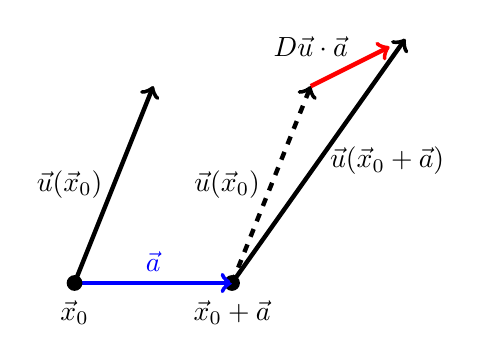
\begin{tikzpicture}
\draw[->,ultra thick] (0,0) -- node[left]{$\vec{u}(\vec{x}_0)$} (1,2.5);

\fill (2,0) circle (1mm);
\node at (2,-0.1) [below] {$\vec{x}_0 + \vec{a} $};
\draw[->,ultra thick,color=blue] (0,0) -- node[above]{$\vec{a}$} (2,0);
\fill (0,0) circle (1mm);
\node at (0,-0.1) [below] {$\vec{x}_0 $};

\draw[->,ultra thick,dashed] (2,0) -- node[left]{$\vec{u}(\vec{x}_0)$} +(1,2.5);
\draw[->,ultra thick,color=red] (2,0) ++(1,2.5) -- ++(1,0.5);
\node at (3,3) {$D \vec{u} \cdot \vec{a}$};

\draw[->,ultra thick] (2,0) -- node[right]{$\vec{u}(\vec{x}_0 + \vec{a})$} ++(2.2,3.1);

\end{tikzpicture}
\caption{The action of the Fr\'{e}chet derivative in $\mathbb{R}^2$.}\label{frechet}
\end{figure}

The correction vector $ D\vec{u} \cdot \vec{a}$ is the tensor dot product of the Fr\'{e}chet derivative with the vector $\vec{a}$. The tensor dot product is defined as
\begin{equation}
\vec{b} = T \cdot \vec{a} ,\quad b_i = T_{ij} a_j
\end{equation}
which is the same as the familiar matrix multiplication of a vector:
\begin{equation}
D \vec{u} \cdot \vec{a} =
\begin{bmatrix}
\partial_x u & \partial_y u \\
\partial_x v & \partial_y v
\end{bmatrix}
\begin{bmatrix}
a_x \\ a_y
\end{bmatrix}
=
\begin{bmatrix}
(\partial_x u) a_x + (\partial_y u) a_y \\
(\partial_x v) a_x + (\partial_y v) a_y
\end{bmatrix}
\end{equation}

$ D\vec{u} \cdot \vec{a}$ is known as the directional derivative of $\vec{u}$ in the direction $\vec{a}$.

\subsubsection{The Velocity Gradient Tensor}
If the vector field is a \emph{velocity} vector field $\vec{u}$, then it is convenient to work with the \textbf{velocity gradient tensor}, denoted $\nabla \vec{u}$.  This is the transpose of the Fr\'{e}chet derivative of the velocity field:
\begin{equation}
\nabla \vec{u} = D\vec{u}^T = 
\begin{bmatrix}
\partial_x u & \partial_x v \\
\partial_y u & \partial_y v
\end{bmatrix}
\end{equation}

This provides a linear approximation to the flow field in the vicinity of $\vec{x}_0$ via:
\begin{equation}
\vec{u}(\vec{x}) \simeq \vec{u}(\vec{x}_0) + (\vec{x} - \vec{x}_0)\cdot \nabla \vec{u}
\end{equation}

This is illustrated in Figure (\ref{velgradtensor}).

\begin{figure}[ht]
\centering
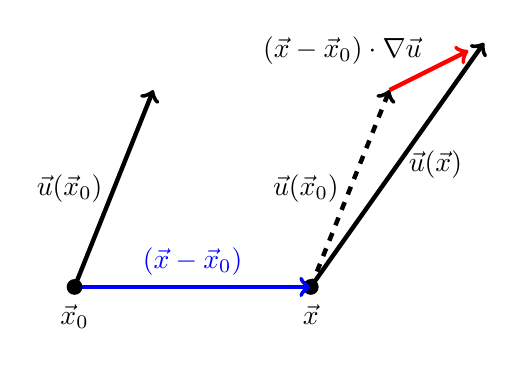
\begin{tikzpicture}
\draw[->,ultra thick] (0,0) -- node[left]{$\vec{u}(\vec{x}_0)$} (1,2.5);

\fill (3,0) circle (1mm);
\node at (3,-0.1) [below] {$\vec{x}$};
\draw[->,ultra thick,color=blue] (0,0) -- node[above]{$(\vec{x} - \vec{x}_0)$} (3,0);
\fill (0,0) circle (1mm);
\node at (0,-0.1) [below] {$\vec{x}_0 $};

\draw[->,ultra thick,dashed] (3,0) -- node[left]{$\vec{u}(\vec{x}_0)$} +(1,2.5);
\draw[->,ultra thick,color=red] (3,0) ++(1,2.5) -- ++(1,0.5);
\node at (3.4,3) {$ (\vec{x} - \vec{x}_0) \cdot \nabla \vec{u}$};

\draw[->,ultra thick] (3,0) -- node[right]{$\vec{u}(\vec{x})$} ++(2.2,3.1);

\end{tikzpicture}
\caption{The action of the velocity gradient tensor.}\label{velgradtensor}
\end{figure}


An advantage of this convention is that the tensor dot product
\begin{equation}
\vec{b} = \vec{a} \cdot T = T^{T} \cdot \vec{a}, \quad b_i = a_j T_{ji}
\end{equation}
allows the notation to follow the form of the familiar one-dimensional case:
\begin{equation*}
f(x) \simeq f(x_0) + (x - x_0) \frac{df}{dx}
\end{equation*}


\vspace*{2em}
An interesting question: how does a vector change in the direction of \emph{the vector itself?} This vector `self gradient' looks like:

\begin{equation}
\vec{u} \cdot \nabla \vec{u}
=
\begin{bmatrix}
u & v
\end{bmatrix}
\begin{bmatrix}
\partial_x u & \partial_x v \\
\partial_y u & \partial_y v
\end{bmatrix}
=
\begin{bmatrix}
u \partial_x u + v \partial_y u \\
u \partial_x v + v \partial_y v
\end{bmatrix}
\end{equation}


Compare this with the \textbf{advection operator}  $(\vec{u} \cdot \nabla ) = u \partial_x + v \partial_y $, operating on vector $\vec{u}$:
\begin{equation}
(\vec{u} \cdot \nabla ) \vec{u} = ( u \partial_x + v \partial_y )
\begin{bmatrix}
u \\ v
\end{bmatrix}
=
\begin{bmatrix}
u \partial_x u + v \partial_y u \\
u \partial_x v + v \partial_y v
\end{bmatrix}
\end{equation}

We see that they are the same.  The advection operator usually appears in the derivation of the `material derivative'.  This alternative derivation via the velocity gradient tensor provides the useful intuition that the advection operator simply gives the change in a vector as one travels in \emph{the direction of the vector itself.} 



\clearpage
\section{Modeling the Bulk Fluid: Navier Stokes}

Fluid is composed of molecules, and the macroscopically observable properties of fluid emerge from the statistical mechanics of \emph{ensembles} of molecules.  Various properties of fluids are described by \emph{continuous} mathematical functions.  Thus, the value of the function at point $\vec{x}$ in a fluid is to be thought of as the statistical mechanical quantity emergent from the ensemble of molecules contained in an infinitesimal \emph{fluid element} located at point $\vec{x}$.
The element -- for clarity, consider it a cube -- is large enough to provide satisfactory statistics for the emergent quantity, but small enough that the continuum approximation is still sound.

\subsubsection{Density}

The density $\rho$ of a fluid is the mass per unit volume of an infinitesimal fluid element.  
It is a scalar quantity that may vary if the fluid is compressible.

\subsubsection{Velocity}

The velocities of the ensemble of molecules in an infinitesimal element can be averaged to define the fluid velocity at that point.  This is true of any point, so the fluid velocity field is a continuous vector-valued function on the fluid. An example is shown in Figure (\ref{bulkfluid}).

\begin{figure}[ht]
\centering
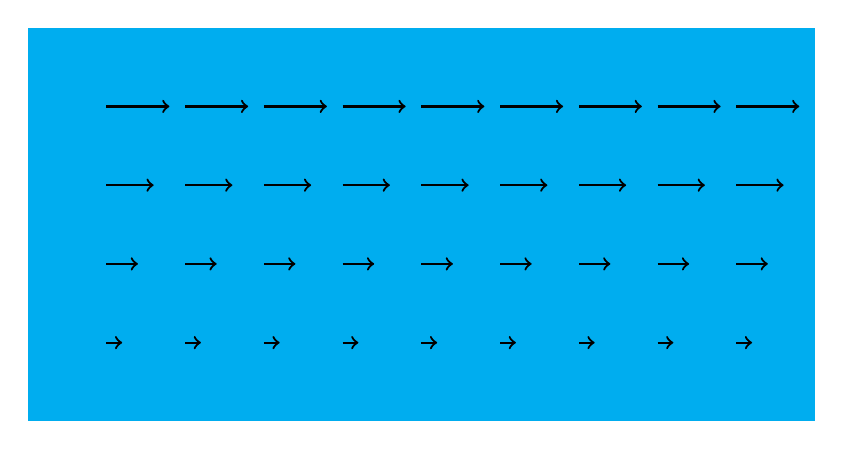
\begin{tikzpicture}

\fill[color=cyan] (0,0) rectangle (10,5);
\foreach \x in {1,2,3,4,5,6,7,8,9}
    \foreach \y in {1,2,3,4}
         \draw[->,thick](\x,\y) -- +(\y/5,0);

\end{tikzpicture}
\caption{A bulk of fluid with a velocity vector field.}\label{bulkfluid}
\end{figure}


\subsection{Incompressible Liquid}

For a vector field, a \textbf{flux} can be defined.  If the fluid is an incompressible liquid, then the flux into a volume element will exactly equal the flux out of the volume element.  This is expressed in the mathematical model by stating that the  divergence of the velocity vector field is zero everywhere:
\begin{equation}
\nabla \cdot \vec{u} = 0
\end{equation}
Incompressibility is a good approximation for liquids, and also turns out to be very mathematically convenient.


\subsubsection{Pressure}

The pressure $p$ is a scalar function defined as the force per unit area acting 
on an arbitrarily oriented plane moving with the fluid.
A pressure gradient in the fluid means that the pressure on one side of a fluid element is higher than on the other side.  This may cause a net force on the fluid element which tends to accelerate it, as suggested in Figure (\ref{pressure}).

\begin{figure}[ht]
\centering
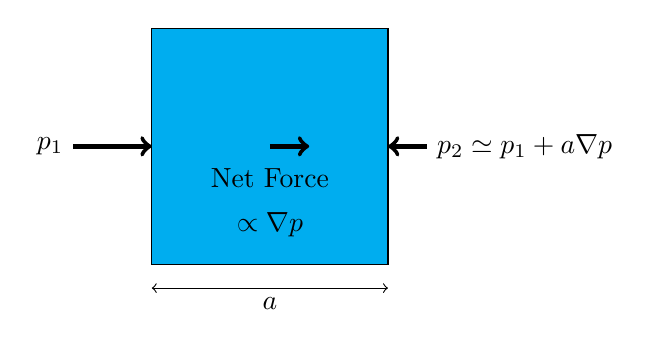
\begin{tikzpicture}

\draw[fill=cyan] (0,0) rectangle (3,3);
\draw[<->] (0,-0.3) -- node[below]{$a$} ++(3,0);

\draw[<-,ultra thick] (0,1.5) -- ++(-1,0);
\draw[<-,ultra thick] (3,1.5) -- ++(0.5,0);
\draw[->,ultra thick] (1.5,1.5) -- ++(0.5,0);

\node at (-1,1.5)[left] {$p_1$};
\node at (3.5,1.5)[right] {$p_2 \simeq p_1 + a \nabla p  $};

\node at (1.5,1.1){Net Force};
\node at (1.5,0.5) {$\propto \nabla p $};

\end{tikzpicture}
\caption{A pressure gradient tends to accelerate a fluid element.}\label{pressure}
\end{figure}


\clearpage
\subsection{Incompressible Viscous Newtonian Fluid}

Interesting fluids have a \emph{viscosity}, $\mu$, an internal friction that allows velocity to propagate through the fluid.  At a molecular level, molecules from a fast fluid element diffuse into an adjacent slower fluid element, and vice versa.  This diffusion of momentum tends to equalise the velocities of adjacent elements.  Thus, viscosity acts with velocity gradients to cause \emph{stresses} on a fluid element caused by the differing velocities of adjacent fluid elements.  If the stresses are balanced, the element will not tend to accelerate, as suggested in Figure (\ref{viscbalance}).

\begin{figure}[ht]
\centering
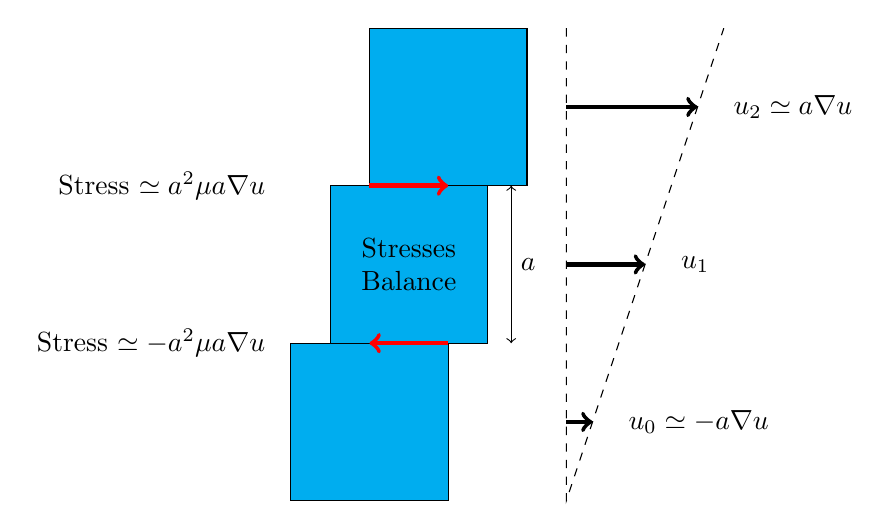
\begin{tikzpicture}

\draw[fill=cyan] (0,0) rectangle ++(2,2);
\draw[fill=cyan] (-0.5,-2) rectangle ++(2,2);
\draw[fill=cyan] (0.5,2) rectangle ++(2,2);
\draw[<->] (2.3,0) -- node [right] {$a$} ++(0,2);

\draw[dashed] (3,4) -- ++(0,-6) -- ++(2,6);
\draw[->,ultra thick] (3,3) -- ++(1.667,0);
\draw[->,ultra thick] (3,1) -- ++(1,0);
\draw[->,ultra thick] (3,-1) -- ++(0.333,0);

\node at (5,3) [right] {$u_2 \simeq a \nabla u $};
\node at (4.333,1) [right] {$u_1$};
\node at (3.667,-1) [right] {$u_0 \simeq - a \nabla u $};

\draw[->,ultra thick, red] (0.5,2) -- ++(1,0);
\draw[<-,ultra thick, red] (0.5,0) -- ++(1,0);

\node at (-0.7,2)[left]{Stress $\simeq a^2 \mu a \nabla u $};
\node at (-0.7,0)[left]{Stress $\simeq - a^2 \mu a \nabla u $};

\renewcommand{\baselinestretch}{1.00}
\node at (1,1)[align=center]{Stresses\\ Balance};

\end{tikzpicture}
\caption{Fluid element at equilibrium with viscous stresses balanced.}\label{viscbalance}
\end{figure}

The velocity gradient gives a linear approximation to the local flow field;
the linearity means that the velocity differences on opposite sides of a fluid element will be equal and opposite.  However, the next level of accuracy is a quadratic approximation using the second derivative of velocity, the Laplacian $\nabla^2 u$.  With the quadratic approximation, there can be a net viscous stress on the fluid element, tending to accelerate it.  This is shown in Figure (\ref{viscacc}). 


\clearpage
\begin{figure}[ht]
\centering
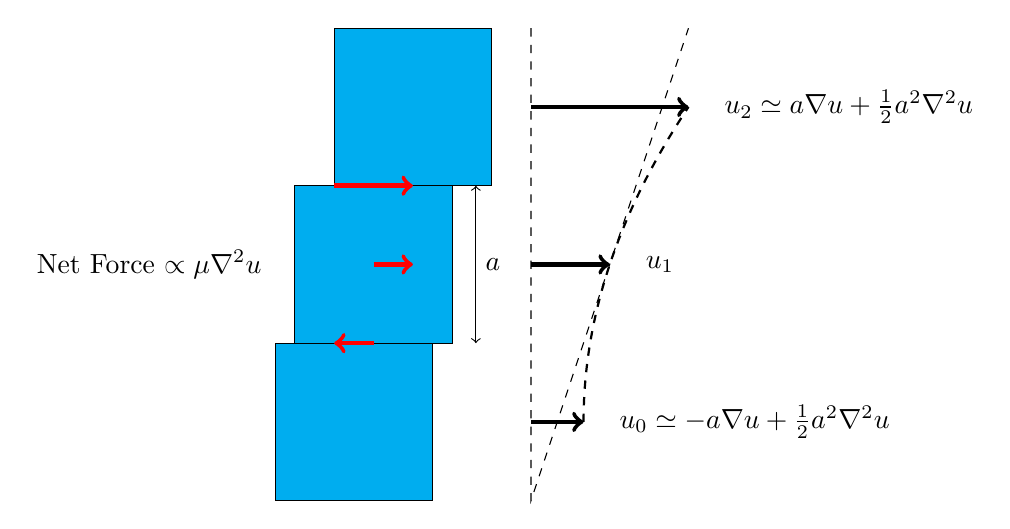
\begin{tikzpicture}

\draw[fill=cyan] (0,0) rectangle ++(2,2);
\draw[fill=cyan] (-0.25,-2) rectangle ++(2,2);
\draw[fill=cyan] (0.5,2) rectangle ++(2,2);
\draw[<->] (2.3,0) -- node [right] {$a$} ++(0,2);

\draw[dashed] (3,4) -- ++(0,-6) -- ++(2,6);
\draw[->,ultra thick] (3,3) -- ++(2,0);
\draw[->,ultra thick] (3,1) -- ++(1,0);
\draw[->,ultra thick] (3,-1) -- ++(0.667,0);

\node at (5.333,3) [right] {$u_2 \simeq a \nabla u + \frac{1}{2}a^2 \nabla^2 u $};
\node at (4.333,1) [right] {$u_1$};
\node at (4,-1) [right] {$u_0 \simeq - a \nabla u + \frac{1}{2}a^2 \nabla^2 u $};

%Bezier curve forced to be quadratic...
\draw[dashed,thick] (3.667,-1) .. controls (3.667,0.333) and (4.111,1.667) .. (5,3);

\draw[->,ultra thick, red] (0.5,2) -- ++(1,0);
\draw[<-,ultra thick, red] (0.5,0) -- ++(0.5,0);

%\node at (-0.7,2)[left]{Stress $\simeq a^2 \mu a \nabla v $};
%\node at (-0.7,0)[left]{Stress $\simeq - a^2 \mu a \nabla v $};

%\renewcommand{\baselinestretch}{1.00}
\draw[->,ultra thick, red](1,1) -- ++(0.5,0);
%\node at (1,1)[align=center]{Net\\ Force};

\node at (-0.3,1)[left]{Net Force $\propto \mu \nabla^2 u$};


\end{tikzpicture}
\caption{Net force on fluid element proportional to $\mu \nabla^2 u$.}\label{viscacc}
\end{figure}

We have seen that a fluid element may be subjected to a net pressure force caused by the pressure gradient $\nabla p$, and a net viscous force caused by the viscosity and velocity laplacian $\nabla^2 u$.  The fluid element has a mass, and the total net force may accelerate the fluid element in accordance with Newton's second law.  This law is embodied in the Navier-Stokes equation.

If no body forces (eg. gravity) are relevant, and the fluid is \textbf{incompressible}, the Navier-Stokes equation is:

\begin{equation}
\rho \left( \frac{\partial \vec{u}}{\partial t} + (\vec{u}\cdot \nabla)\vec{u} \right) = -\nabla p +  \mu \nabla^2 \vec{u}
\end{equation}

If the equation is multiplied by the volume of the infinitesimal fluid element, then
the left-hand side is the acceleration, and the right-hand side is the force due to the pressure gradient and viscous shear.  The `advection operator'
 $(\vec{u} \cdot \nabla ) = u \partial_x + v \partial_y $
 gives the `inertial' term  $ (\vec{u}\cdot \nabla)\vec{u} $.


\clearpage
\section{Microfluidics: Stokes or `creeping' flow}


The Navier-Stokes equations are an excellent description of much fluid flow.  However, the advection terms like $u \partial_x u$ in the differential equation are not linear, in the sense
that they cannot be put in the form $\dotsb + a_0 u + a_1 \partial_x u + \dotsb$.  Nonlinear partial differential equations are notoriously difficult to solve.  But there is hope.  In some physical cases, the nonlinear terms may be much smaller than the rest, and contribute only a negligible amount to the solution.  In that case, the nonlinear terms can be discarded, and the solution of the resulting linear equation is a very good approximation.  We will now show that this is true for the microfluidic case where slip effects are noticeable.

One way to compare the relative magnitudes of the terms is to first non-dimensionalise the terms. The idea is this: express the fundamental physical quantities as fractions of a `characteristic' value. The fraction forms a new, dimensionless variable. Then typical values of the dimensionless variables have a magnitude on the order of one.  For example, consider Poiseuille flow down a straight pipe, where the average velocity is $U$.  The velocity $u$ varies from zero at the wall, to  $\frac{3}{2} U$ in the centre of the pipe.  Now define the dimensionless velocity $\hat{u} = u/U$.  Clearly, the magnitude of $\hat{u}$ will vary from zero at the wall, to $\frac{3}{2}$ in the centre. i.e. for most of the domain, $\hat{u}$ is `about one'.

A non-dimensionalised equation will hopefully have many terms with a magnitude on the order of one, with the magnitude of the remaining terms easily evaluated.  Thus, non-dimensionalising expedites the process of deciding which terms are negligible enough to discard.


%Poiseuille flow in pipe ($R$ is pipe radius) to put in somewhere:
%\begin{equation}
%u(r) = - \frac{1}{4\eta} \frac{\Delta p}{\Delta x} \left( R^2 - r^2 \right)
%\end{equation}

\clearpage
\subsection{Non-dimensionalising and the Reynolds Number}
\subsubsection{Example for Analysis: 2-D Poiseuille Flow}
This thesis analyses microfluidic flow experiments that reveal slip effects.  The canonical flow experiment is flow down a capillary --- a very thin pipe or channel.  
We shall use this type of flow to analyse our non-dimensionalisation.  For clarity, we shall stick to two dimensions; this models pressure-driven flow between two infinite flat planes separated by distance $L$.
% This avoids messing about with cylindrical coordinates.
This is known as plane Poiseuille flow.  The solution is a parabolic velocity profile, the same as for Poiseuille flow as found in a straight, circular pipe:

\begin{equation}
u(y) = \frac{1}{2 \mu} \left( \frac{dp}{dx} \right) \left( y^2 - yL \right)
\end{equation}

The standard way to non-dimensionalise pipe flow is to choose the pipe diameter $L$ as the characteristic length.  Likewise, we choose channnel width $L$, and average velocity $U$ as the characteristic velocity.


Then the non-dimensional variables are:
\begin{equation}
\hat{x} = \frac{x}{L}, \quad \hat{y} = \frac{y}{L}, \quad
 \hat{u} = \frac{u}{U}, \quad \hat{v} = \frac{v}{U}
\end{equation}

The other variables are pressure and time.  We would like to express them in terms of existing quantities.
It turns out that $ \mu U / L $ has units of pressure, and the ratio $L /U$ has units of time, so define characteristic pressure and time:
\begin{equation}
P = \frac{\mu U}{L}, \quad T = \frac{L}{U}
\end{equation}
giving dimensionless variables $\hat{p} = p/P$ and $\hat{t}=t/T$:
\begin{equation}
\hat{p} = \frac{L}{\mu U} p, \quad \hat{t} = \frac{U}{L}t
\end{equation}

Thus we can substitute
\begin{equation}
x = L\hat{x}, \quad y = L\hat{y}, \quad u = U \hat{u}, \quad v = U \hat{v}, 
\quad p = \frac{\mu U}{L}\hat{p}, \quad t = \frac{L}{U}\hat{t}
\end{equation}
into the Navier-Stokes equation.  For clarity, we focus on just the $x$ component:
\begin{equation}
\rho \left( \frac{\partial u}{\partial t} +
 u \frac{\partial u}{\partial x} + v\frac{\partial u}{\partial y} \right) =
 - \frac{\partial p}{\partial x} + 
\mu \left( \frac{\partial^2 u}{\partial x^2} + \frac{\partial^2 u}{\partial y^2} \right)
\end{equation}

Substitute:
\begin{equation}
\rho \left( \frac{\partial U\hat{u}}{\partial \frac{L}{U}\hat{t}} +
U\hat{u} \frac{\partial U\hat{u}}{\partial L\hat{x}} +
U\hat{v} \frac{\partial U\hat{u}}{\partial L\hat{y}} \right) =
 - \frac{\partial \frac{\mu U}{L} \hat{p}}{\partial L\hat{x}} + 
\mu \left( \frac{\partial^2 U\hat{u}}{\partial (L\hat{x})^2} + 
\frac{\partial^2 U\hat{u}}{\partial (L\hat{y})^2} \right)
\end{equation}

\begin{equation}
\rho \frac{U^2}{L} \left( \frac{\partial \hat{u}}{\partial \hat{t}} +
\hat{u} \frac{\partial \hat{u}}{\partial \hat{x}} +
\hat{v} \frac{\partial \hat{u}}{\partial \hat{y}} \right) =
 - \frac{\mu U}{L^2} \frac{\partial \hat{p}}{\partial \hat{x}} + 
\frac{\mu U}{L^2} \left( \frac{\partial^2 \hat{u}}{\partial \hat{x}^2} + 
\frac{\partial^2 \hat{u}}{\partial \hat{y}^2} \right)
\end{equation}

%\begin{equation}
%\text{Now multiply both sides by} \quad \frac{L^2}{\mu U}
%\end{equation}

\begin{equation}
\frac{\rho L U}{\mu} \left( \frac{\partial \hat{u}}{\partial \hat{t}} +
\hat{u} \frac{\partial \hat{u}}{\partial \hat{x}} +
\hat{v} \frac{\partial \hat{u}}{\partial \hat{y}} \right) =
 -  \frac{\partial \hat{p}}{\partial \hat{x}} + 
\left( \frac{\partial^2 \hat{u}}{\partial \hat{x}^2} + 
\frac{\partial^2 \hat{u}}{\partial \hat{y}^2} \right)
\end{equation}


\vspace{1em}
Define Kinematic Viscosity
\begin{equation}
\nu = \frac{\mu}{\rho}
\end{equation}
Then define the \textbf{Reynolds Number:}
\begin{equation}
\mathrm{Re} = \frac{L U}{\nu}
\end{equation}

Thus the $x$ component of the Navier-Stokes equations are:
\begin{equation}
\mathrm{Re} \left( \frac{\partial \hat{u}}{\partial \hat{t}} +
\hat{u} \frac{\partial \hat{u}}{\partial \hat{x}} +
\hat{v} \frac{\partial \hat{u}}{\partial \hat{y}} \right) =
 -  \frac{\partial \hat{p}}{\partial \hat{x}} + 
\left( \frac{\partial^2 \hat{u}}{\partial \hat{x}^2} + 
\frac{\partial^2 \hat{u}}{\partial \hat{y}^2} \right)
\end{equation}


\vspace{1em}
We are now in a position to look at the relative magnitudes of the terms.

\clearpage
\subsubsection{Magnitudes of Velocity Terms}



We have chosen Poiseuille flow to illustrate our non-dimensionalisation.  Since it has an exact solution, we know exactly what the velocity and its derivatives are.
%  With average velocity scaled to unity, and channel width also scaled to unity, 
The parabolic velocity profile looks as shown in Figure (\ref{poise}).

\begin{figure}[ht]
\centering
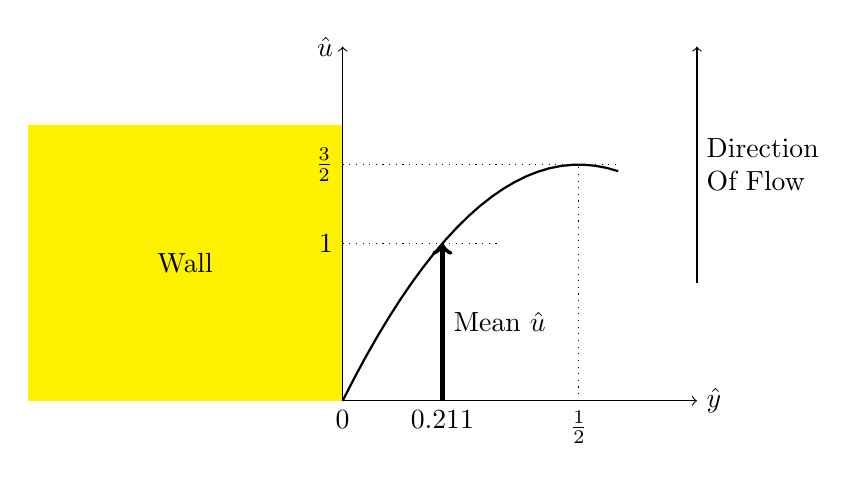
\begin{tikzpicture}
\fill [color=yellow] (0,0) rectangle node [color=black] {Wall}(-4,3.5);

\draw[->] (0,0) -- (0,4.5);
\draw[->] (0,0) -- (4.5,0);
\node at (0,4.5)[left]{$ \hat{u} $};
\node at (4.5,0)[right]{$\hat{y}$};

\node at(0,0) [below] {0};
\draw [dotted] (3,0) -- ++(0,3);
\node at (3,0)[below] {$\frac{1}{2}$};
\draw [dotted] (0,2) -- ++ (2,0);
\node at (0,2)[left] {1};
\draw [dotted] (0,3) -- ++(3.5,0);
\node at (0,3) [left] {$\frac{3}{2}$};

\draw[thick] plot [domain = 0:3.5](\x, {3 - 0.3333*((\x - 3)^2)}  );

\draw[ultra thick,->] (1.266,0) -- node[right]{Mean $\hat{u}$} ++(0,2);
\node at (1.266,0) [below] {0.211};

\renewcommand{\baselinestretch}{1.00}
\draw [->](4.5,1.5) -- node[right,align=left]{Direction\\ Of Flow} ++(0,3);

\end{tikzpicture}
\caption{Dimensionless parabolic flow profile of plane Poiseuille flow.}\label{poise}
\end{figure}


By construction, the $\hat{u}$ term ranges from zero to $\frac{3}{2}$. Hence, $\hat{u}$ is of order one.

For \emph{strict} Poiseuille flow, the walls are perfectly flat, and the velocity perpendicular to the wall is zero everywhere.  That is, $\hat{v} = 0$ always. 

But we may consider a channel with roughness on the walls, with the amplitude of the roughness \emph{small} compared to the channel width, so that the flow is Poiseuille-like.  Then, near the wall, the transverse velocity $\hat{v}$ may approach the magnitude of $\hat{u}$.  The magnitude of $\hat{u}$ near the wall is small compared to the average, so we would expect perhaps $\hat{v} < 0.1$.  That is, for rough-walled Poiseuille-like flow, $\hat{v}$ is of order 0.1, at most.


\subsubsection{Magnitudes of Velocity Derivative Terms}

A typical capillary flow experiment is carried out with flow rates held constant, and at low enough flow velocities that the flow is laminar.
For the purposes of our analysis, we shall assume steady non-turbulent flow,
so the time-dependent velocity term vanishes.
\begin{equation}
\frac{\partial \hat{u}}{\partial \hat{t}} = 0
\end{equation}


For the parabolic flow profile of Poiseuille flow, the derivative of velocity is linear, as shown in Figure (\ref{poisedrv1}).
\begin{figure}[ht]
\centering
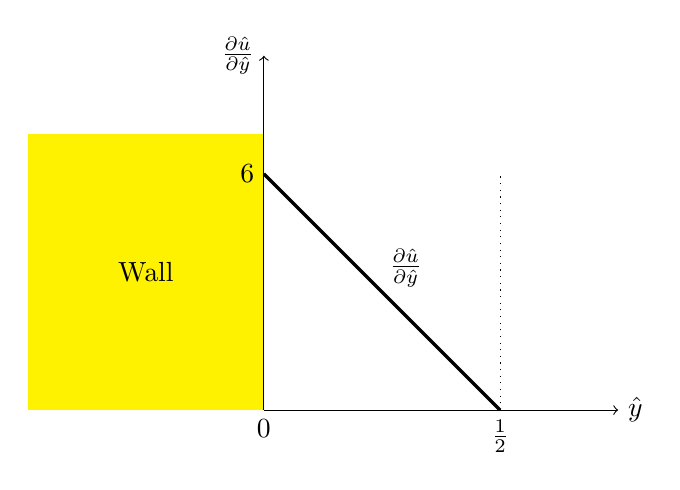
\begin{tikzpicture}
\fill [color=yellow] (0,0) rectangle node [color=black] {Wall}(-3,3.5);

\draw[->] (0,0) -- (0,4.5);
\draw[->] (0,0) -- (4.5,0);
\node at (0,4.5)[left]{$ \frac{\partial \hat{u}}{\partial \hat{y}} $};
\node at (4.5,0)[right]{$\hat{y}$};

\node at(0,0) [below] {0};
\node at (3,0)[below] {$\frac{1}{2}$};
\draw [dotted] (3,0) -- ++(0,3);

\node at (0,3) [left] {6};

\draw [very thick] (0,3) -- (3,0);
\node at (1.8,1.8) {$\frac{\partial \hat{u}}{\partial \hat{y}} $};

\end{tikzpicture}
\caption{Velocity first derivative of plane Poiseuille flow.}\label{poisedrv1}
\end{figure}

The average \emph{value} of $\partial_y \hat{u}$ over the channel width is zero.  But the average \emph{magnitude} is 3.  
%In the tradition of theoretical physics,
So $\partial_{\hat{y}} \hat{u}$ is `of order one'.

For strict Poiseuille flow, $\hat{u}$ has no $x$-dependence, so $\partial_{\hat{x}} \hat{u} = 0$ everywhere.

%For rough-walled Poiseuille-like flow, the wall corrugations will cause the $x$ velocity to change in the $x$ direction, over the period of the corrugation.
% The $x$ velocity in the vicinity of the wall is on the order of 0.1, and varies by perhaps 10\% over the roughness period. 
%  The roughness period must very small compared with the channel width for the flow to remain Poiseuille-like. 
% Thus, in the vicinity of the wall, $\partial_{\hat{x}} \hat{u} \sim (0.1 \times 0.1) / 0.01 = 1$.  But for the rest of the domain, the $x$ velocity will have vanishing $x$ dependence.  So \emph{average} $\partial_{\hat{x}} \hat{u}$ is more like 0.1.  Hence, $\partial_{\hat{x}} \hat{u}$ is of order 0.1.

But for rough-walled Poiseuille flow, the wall corrugations will cause velocity $\hat{u}$ near the wall to change in the $x$ direction, over the period of the corrugation.  Near the wall, $\hat{u}$ is on the order of 0.1 or less, so $\Delta \hat{u}$ over the period can be no more than 0.1.  For the flow to remain Poiseuille-like, the roughness period must be small compared to the channel width, i.\ e.\ on the order of 0.1 or less. Thus, in the vicinity of the wall, $\partial_{\hat{x}} \hat{u} \sim 0.1 / 0.1 = 1$.  Away from the wall, $\partial_{\hat{x}} \hat{u}$ becomes smaller as flow converges on strict Poiseuille flow.  Thus, $\partial_{\hat{x}} \hat{u}$ is of order one, at most.


\subsubsection{Magnitudes of Advection Terms}

%With $\hat{u}$ of order one and $\partial_{\hat{x}} \hat{u}$ of order 0.1, and $\hat{v}$ of order 0.1 and $\partial_{\hat{y}} \hat{u}$ of order one, the advection terms $\hat{u} \partial_{\hat{x}} \hat{u}$ and $\hat{v} \partial_{\hat{y}} \hat{u}$ are both of order 0.1.

$\partial_{\hat{x}} \hat{u}$ vanishes over the middle part of the domain (where $\hat{u}$ is at most $3/2$) and reaches a maximum of about 1 near the wall, where $\hat{u}$ is of order 0.1.  Therefore, $\hat{u} \partial_{\hat{x}} \hat{u}$ is at most 0.1.

Near the wall, both $\hat{v}$ and $\partial_{\hat{y}} \hat{u}$ are at their maxima: $\hat{v} \sim 0.1$ and $\partial_{\hat{y}} \hat{u} \sim 5 $. Their product is about 0.5, or order 1.  Thus, $\hat{v} \partial_{\hat{y}} \hat{u}$ is of order one, at most.

\subsubsection{Magnitudes of Second Derivatives of Velocity}

The second spatial derivative of the parabolic velocity profile is a constant, as illustrated in Figure (\ref{poiselap}).
\begin{figure}[ht]
\centering
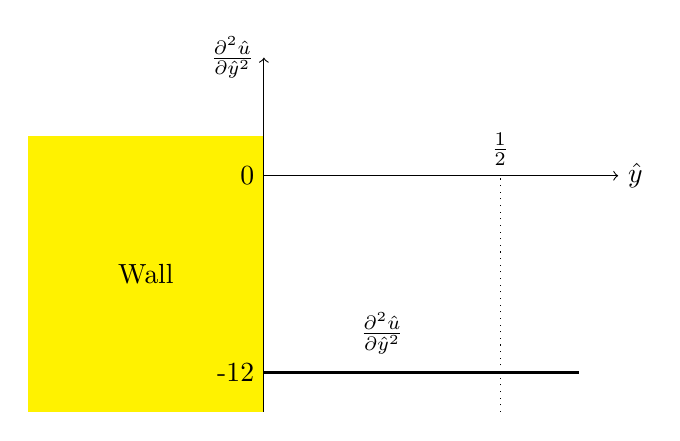
\begin{tikzpicture}
\fill [color=yellow] (0,0) rectangle node [color=black] {Wall}(-3,3.5);

\draw[->] (0,0) -- ++(0,4.5);
\draw[->] (0,3) -- ++(4.5,0);

\node at (0,4.5)[left]{$ \frac{\partial^2 \hat{u}}{\partial \hat{y}^2} $};
\node at (4.5,3)[right]{$\hat{y}$};

\node at (3,3)[above] {$\frac{1}{2}$};
\draw [dotted] (3,0) -- ++(0,3);

\node at (0,3) [left] {0};

\node at (0,0.5) [left] {-12};
\draw [very thick] (0,0.5) -- ++(4,0);
\node at (1.5,1) {$\frac{\partial^2 \hat{u}}{\partial \hat{y}^2} $};

\end{tikzpicture}
\caption{Velocity Laplacian of plane Poiseuille flow.}\label{poiselap}
\end{figure}

For Poiseuille flow nondimensionalized in the standard way, $ \frac{\partial^2 \hat{u}}{\partial \hat{y}^2} = -12$.  That is, the magnitude is of order ten.

For strictly Poiseuille flow, the $x$ velocity has no $x$ dependence, so $\partial_{\hat{x}} \hat{u} = 0 $, and $ \partial^2_{\hat{x}} \hat{u} = 0 $.

For rough-walled Poiseuille-like flow, we have allowed that $\partial_{\hat{x}} \hat{u} \sim 1$ for the 10\% of the domain near the wall.  This reduces to near zero for the rest of the domain.  Therefore, $\partial_{\hat{x}} \hat{u}$ reduces from order one to zero in distance 0.1, hence average $ \partial^2_{\hat{x}} \hat{u}$ \emph{near the wall} is of order ten.  
%But it is zero over the rest of the domain, so the average over the channel is one.
Hence, $ \partial^2_{\hat{x}} \hat{u}$ is of order ten at most.

%\vspace{1em}
%And now to the pressure term:  The characteristic pressure $P$ was chosen for dimensional convenience, not because it is necessarily a typical pressure.  So it is impossible to know the magnitude of $\hat{p}$ or $\partial_{\hat{x}} \hat{p}$.  But this doesn't matter; we have enough information to simplify, as we shall see.

\subsubsection{Summary of Magnitudes of Terms}

At this point, we can summarize what we know about the relative magnitudes of the terms in the Navier-Stokes equation.  For steady strict Poiseuille flow nondimensionalized in the standard way, the velocity $\hat{u}(x,y)$ in the direction of the flow obeys:
\begin{equation}
\mathrm{Re} \left( 
\underbrace{ \frac{\partial \hat{u}}{\partial \hat{t}} }_{\text{= 0}} +
\underbrace{ \hat{u} \frac{\partial \hat{u}}{\partial \hat{x}} }_{\text{= 0}} +
\underbrace{ \hat{v} \frac{\partial \hat{u}}{\partial \hat{y}} }_{\text{= 0}} 
\right) = 
\underbrace{ - \frac{\partial \hat{p}}{\partial \hat{x}} }_{\text{unknown}}
  + \left( 
\underbrace{ \frac{\partial^2 \hat{u}}{\partial \hat{x}^2} }_{\text{= 0}} + 
\underbrace{ \frac{\partial^2 \hat{u}}{\partial \hat{y}^2} }_{\sim 10} 
\right)
\end{equation}
Which simplifies considerably to:
\begin{equation}
0 = -  \frac{\partial \hat{p}}{\partial \hat{x}} + 
%\left( \frac{\partial^2 \hat{u}}{\partial \hat{x}^2} + 
\frac{\partial^2 \hat{u}}{\partial \hat{y}^2} % \right)
\end{equation}

But for rough-walled Poiseuille-like flow, things are not quite so simple:
\begin{equation}
\mathrm{Re} \left( 
\underbrace{ \frac{\partial \hat{u}}{\partial \hat{t}} }_{\text{= 0}} +
\underbrace{ \hat{u} \frac{\partial \hat{u}}{\partial \hat{x}} }_{\sim 0.1} +
\underbrace{ \hat{v} \frac{\partial \hat{u}}{\partial \hat{y}} }_{\sim 1} 
\right) = 
\underbrace{ - \frac{\partial \hat{p}}{\partial \hat{x}} }_{\text{unknown}}
  + \left( 
\underbrace{ \frac{\partial^2 \hat{u}}{\partial \hat{x}^2} }_{\sim 10} + 
\underbrace{ \frac{\partial^2 \hat{u}}{\partial \hat{y}^2} }_{\sim 10} 
\right)
\end{equation}

That is:
\begin{equation}
\mathrm{Re} \left( 
\underbrace{ \frac{\partial \hat{u}}{\partial \hat{t}}  +
     \hat{u} \frac{\partial \hat{u}}{\partial \hat{x}}  +
     \hat{v} \frac{\partial \hat{u}}{\partial \hat{y}} }_{\text{order 1}} 
\right) = 
\underbrace{ - \frac{\partial \hat{p}}{\partial \hat{x}} }_{\text{unknown}}
  + \left( 
\underbrace{ \frac{\partial^2 \hat{u}}{\partial \hat{x}^2} }_{\sim 10} + 
\underbrace{ \frac{\partial^2 \hat{u}}{\partial \hat{y}^2} }_{\sim 10} 
\right)
\end{equation}

%\begin{equation}
%\mathrm{Re} \left( 
%\underbrace{ \frac{\partial \hat{u}}{\partial \hat{t}}  +
%     \hat{u} \frac{\partial \hat{u}}{\partial \hat{x}}  +
%     \hat{v} \frac{\partial \hat{u}}{\partial \hat{y}} }_{\text{order 0.1}} 
%\right) = 
%\underbrace{ - \frac{\partial \hat{p}}{\partial \hat{x}}
% + \left( 
%          \frac{\partial^2 \hat{u}}{\partial \hat{x}^2}  + 
%          \frac{\partial^2 \hat{u}}{\partial \hat{y}^2}
%  \right) }_{\text{order at least 10}}
%\end{equation}

Importantly, we have discovered the relative magnitudes of the terms that \emph{do not depend on the physical situation.}  The above relation holds for Poiseuille flow of \emph{any} fluid at \emph{any} scale.  The parameters pertaining to the specific physical system are wrapped up into the Reynolds number.

Now is a good time, then, to evaluate the Reynolds number for the kind of microfluidic slip experiments we are considering.

\subsubsection{Reynolds number for microfluidic channels}

A recent Poiseuille-type microfluidic slip experiment appears in the 2006 paper by Huang \emph{et al} in the Journal of Fluid Mechanics \cite{Huang2006}.  They looked at steady flow in channels 50 $\mu$m deep and 250 $\mu$m wide.  Particle velocimetry techniques showed a velocity distribution with a maximum velocity of about 600 $\mu$m s$^{-1}$.
When defining the Reynolds number for flow in a rectangular duct, the standard characteristic length to use is the \textbf{hydraulic diameter}, which is four times the cross-sectional area divided by the perimeter.  In this case it is 83.33 $\mu$m.
%$(4 \times 50 \times 250) / (50 + 250 + 50 + 250)$ which is 83.33 $\mu$m.

The viscosity of water at room temperatures is very close to $\mu = 0.001$ kgs$^{-1}$m$^{-1}$.  The density of water is $\rho = 1000$ kgm$^{-3}$.  We shall choose $L = 100 \mu$m and $U = 400 \mu$m s$^{-1}$ as conservative characteristic length and velocity scales.
Hence the Reynolds number evaluates to:
\begin{equation}
\mathrm{Re} = \frac{\rho L U}{\mu} = \frac{1000 \times 0.0001 \times 0.004}{0.001} = 0.4
\end{equation}
%In the tradition of theoretical physics, this may be described as `of order 0.1'.
%Thus the magnitudes of the two sides of the Navier-Stokes equation are:
%\begin{equation}
%\underbrace{
%\mathrm{Re} \left( 
%             \frac{\partial \hat{u}}{\partial \hat{t}}  +
%     \hat{u} \frac{\partial \hat{u}}{\partial \hat{x}}  +
%     \hat{v} \frac{\partial \hat{u}}{\partial \hat{y}} 
%           \right)
%}_{\text{order 0.04}}   = 
%\underbrace{ - \frac{\partial \hat{p}}{\partial \hat{x}}
% + \left( 
%          \frac{\partial^2 \hat{u}}{\partial \hat{x}^2}  + 
%          \frac{\partial^2 \hat{u}}{\partial \hat{y}^2}
%  \right) }_{\text{order at least 10}}
%\end{equation}
%
%So the right-hand side of the equation is \emph{at least} 250 times bigger than the left-hand side.  We have achieved our goal of finding which terms are negligible enough to discard.  We boldly make the tactical decision to throw away the left hand side, and solve instead the much simpler equation:
Thus the magnitudes of terms in the Navier-Stokes equation are:
\begin{equation}
\underbrace{
\mathrm{Re} \left( 
             \frac{\partial \hat{u}}{\partial \hat{t}}  +
     \hat{u} \frac{\partial \hat{u}}{\partial \hat{x}}  +
     \hat{v} \frac{\partial \hat{u}}{\partial \hat{y}} 
           \right)
}_{\text{order 0.4}}   = 
\underbrace{ - \frac{\partial \hat{p}}{\partial \hat{x}} }_{\text{unknown}}
  + \left( 
\underbrace{ \frac{\partial^2 \hat{u}}{\partial \hat{x}^2} }_{\sim 10} + 
\underbrace{ \frac{\partial^2 \hat{u}}{\partial \hat{y}^2} }_{\sim 10} 
\right)
\end{equation}

%The entire left-hand side evaluates to something with a magnitude less than one.  On the right-hand side, there is a term with a magnitude always greater than 10, a term  whose magnitude is at most 10, and a term of unknown magnitude.
The three terms on the right-hand side sum up to something with a magnitude at least 25 times smaller than the largest term on the right.
That is, the equation is `close to' the similar equation in which the the right-hand side terms sum to \emph{zero.}  Thus, we choose to solve the much simpler equation: 
\begin{equation}
0 = -  \frac{\partial \hat{p}}{\partial \hat{x}} + 
\left( \frac{\partial^2 \hat{u}}{\partial \hat{x}^2} + 
\frac{\partial^2 \hat{u}}{\partial \hat{y}^2} \right)
\end{equation}

The $y$ component of the Navier-Stokes is:
\begin{equation}
\mathrm{Re} \left( 
\frac{\partial \hat{v}}{\partial \hat{t}} +
\hat{u} \frac{\partial \hat{v}}{\partial \hat{x}} +
\hat{v} \frac{\partial \hat{v}}{\partial \hat{y}}
 \right) =
    -  \frac{\partial \hat{p}}{\partial \hat{y}} + 
\left( \frac{\partial^2 \hat{v}}{\partial \hat{x}^2} + 
       \frac{\partial^2 \hat{v}}{\partial \hat{y}^2} 
\right)
\end{equation}
For pure Poiseuille flow, this reduces to 0 = 0.  For rough-walled Poiseuille-like flow, we expect $\hat{v}$ to be nonzero but very small compared to $\hat{u}$.  
So we anticipate no significant loss of information if we discard the left-hand side of the $y$ velocity equation.  If we do this, then we have simplified the Navier-Stokes vector equation to:
\begin{equation}
0 = -\hat{\nabla} \hat{p} + \hat{\nabla}^2 \hat{\vec{u}}
\end{equation}
or
\begin{equation}
\hat{\nabla}^2 \hat{\vec{u}} = \hat{\nabla} \hat{p}
\end{equation}
This is known as the Stokes equation, and describes very slow-moving flow described as `creeping' flow or Stokes flow.  Stokes flow is associated with Reynolds numbers Re $ \ll 1$.  Some perspective: for flow in a pipe, flows with Reynolds numbers below about 2,300 are always laminar, while flows with Reynolds numbers above about 4,000 are always turbulent.

In Stokes flow, the time-dependent and inertial terms are deemed to be negligible compared to the pressure and viscosity terms.  Thus, the Stokes equation describes the force balance between pressure and viscous stresses.

\subsection{Redimensionalize back to Physical Units}

We will convert back into physical units. Substituting the definitions of the dimensionless variables back into the Stokes equation:
\begin{equation}
\left( \frac{\partial^2  \frac{u}{U}}{\partial (\frac{x}{L})^2} + 
\frac{\partial^2 \frac{u}{U}}{\partial (\frac{y}{L})^2} \right) =
\frac{\partial \frac{L}{\mu U} p}{\partial \frac{x}{L}}
\end{equation}

\begin{equation}
 \frac{L^2}{\mu U} \left( \frac{\partial^2 u}{\partial x^2} + 
\frac{\partial^2 u}{\partial y^2} \right) =
\frac{L^2}{\mu U}  \frac{\partial p}{\partial x}
\end{equation}

%\begin{equation}
%\text{Multiply both sides by} \quad \frac{\mu U}{L^2}
%\end{equation}

\begin{equation}
\mu \left( \frac{\partial^2 u}{\partial x^2} + 
\frac{\partial^2 u}{\partial y^2} \right) =
\frac{\partial p}{\partial x}
\end{equation}

Similarly for the other vector components of the Stokes equation.

\vspace*{1em}
Thus, for microfluidic flow down a capillary, the bulk fluid obeys the Stokes equation:
\begin{equation}
\mu \nabla^2 \vec{u} = \nabla p
\end{equation}

In the field of microfluidics, it is customary to assume Stokes flow in all cases. However, we note that for example, the capillary slip experiment of Vinogradova 2009 \cite{Vinogradova2009} had velocities of up to 5 cm per second down a channel 100 $\mu$m wide, yielding a Reynolds number Re $\sim$ 1.
%  This makes the pressure and shear force terms only ten times larger than the inertial terms, so some error may be noticeable.
%But, we shall follow the custom of microfluidics, and assume Stokes flow holds in the bulk.


%Vinogradova PRL 2009 had velocities up to 5 cm per second. Then Re = 1.  Too big.  Stokes %flow only sensible if Re $\ll$ 1.  Eg. Re $<$ 0.1.



\section{Modeling the Boundary: Generalized Slip}

%After establishing that the Stokes equation holds in the bulk fluid, we turn now to the boundary.  The first order of business is to define \emph{where} the boundary is.  As the discussion in Chapter 2 showed, there is some ambiguity about the location of the nominal boundary.  For a true physical surface, there may be a \emph{region} of finite width that could be labelled the `boundary'.  At the top of the region, the bulk fluid behaviour obtains, and at the bottom of the boundary, it is unambiguously solid.  

%We are constructing a mathematical model of a physical system; in the model there will be a boundary that is a purely geometric surface (of zero width), and at any arbitrary distance above the boundary, the bulk fluid conditions will hold.  We need to decide exactly which part of the physical boundary region maps to our model boundary.  The sensible choice is: the top.

%Here is why: As we descend down through the fluid towards the physical boundary, there will be a point at which the local conditions begin to deviate from that of the bulk.  Perhaps the density changes --- we are entering a `depletion region' with correspondingly lower viscosity.  In the mathematical model, there is a perfect distinction between `bulk' and `boundary'.  Thus we must identify the mathematical boundary with the very top of the physical boundary region.

After establishing that the Stokes equation and incompressibility condition hold in the bulk region (domain) of our model, we now turn to the boundary.  There may be some subtlety as to \emph{where} the boundary is, in the following sense: In the mathematical model we are constructing, the distinction between bulk and boundary has the perfect discontinuity of a geometric object.  However, as noted earlier, in a physical system, there may be some ambiguity as to what constitutes the boundary; there may be a \emph{region} of finite depth that could reasonably be called the boundary region.  The question then is: what part of the boundary region of the physical system corresponds to the boundary surface in the mathematical model?

The justifiable choice is for the mathematical boundary to map to the \emph{top} of the physical boundary region.  In the physical system, certain conditions hold that are homogeneous through the bulk of the fluid.  However, near the surface, there may be some deviation from these conditions (caused perhaps by a depletion layer).  This is not allowed in the mathematical model (since in the model, the domain is homogeneous), so the mathematical boundary must map to the lowest part of the homogeneous physical bulk region.  This is illustrated in Figure (\ref{boundarymap}).

\begin{figure}[ht]
\centering
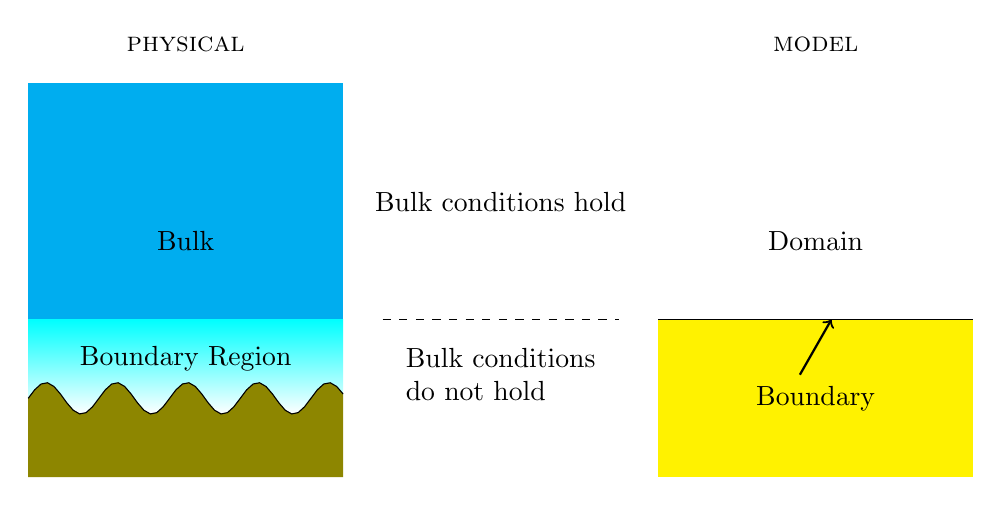
\begin{tikzpicture}
\fill[color=cyan] (0,0) rectangle (4,3);
\shade[top color=cyan](0,0) rectangle (4,-1.2);

\node at (2,1) {Bulk};
\node at (2,-0.5){Boundary Region};

\fill [color=olive,domain=0:4,samples=50] plot (\x,{ 0.2 * sin(7*\x r) - 1} ) -- (4,-2) -- ++(-4,0);
\draw [domain=0:4,samples=50] plot (\x,{ 0.2 * sin(7*\x r) - 1} );


\fill[color=yellow](8,0) rectangle ++(4,-2);
\draw(8,0) -- ++(4,0);
\node at (10,1) {Domain};
\node at (10,-1) {Boundary};
\draw[->,thick] (9.8,-0.7) -- (10.2,0);

\node at (2,3.5) {\textsc{physical}};
\node at (10,3.5) {\textsc{model}};

\node at (6,1.5) {Bulk conditions hold};
\draw[dashed] (4.5,0) -- ++(3,0);
\renewcommand{\baselinestretch}{1.00}
\node at (6,-0.7) [align=left]{Bulk conditions\\ do not hold};

\end{tikzpicture}
\caption{Model boundary maps to \emph{top} of physical boundary region.}\label{boundarymap}
\end{figure}

\clearpage
\subsection{Simple Shear with Navier Slip}

As explained in the introductory chapters, the classical boundary condition is `no slip', and the simplest extension to that is Navier slip, where the boundary velocity is proportional to the velocity gradient:
\begin{equation}
u_{\text{boundary}} = b \frac{\partial u}{\partial z} \bigg|_{\text{boundary}}
\end{equation}

This holds for a system exhibiting \textbf{simple shear:} a flat surface with laminar flow above it, with each lamina parallel to the boundary surface.  There is no velocity component normal to the surface.  See Figure (\ref{simpleshear}).

\begin{figure}[ht]
\centering
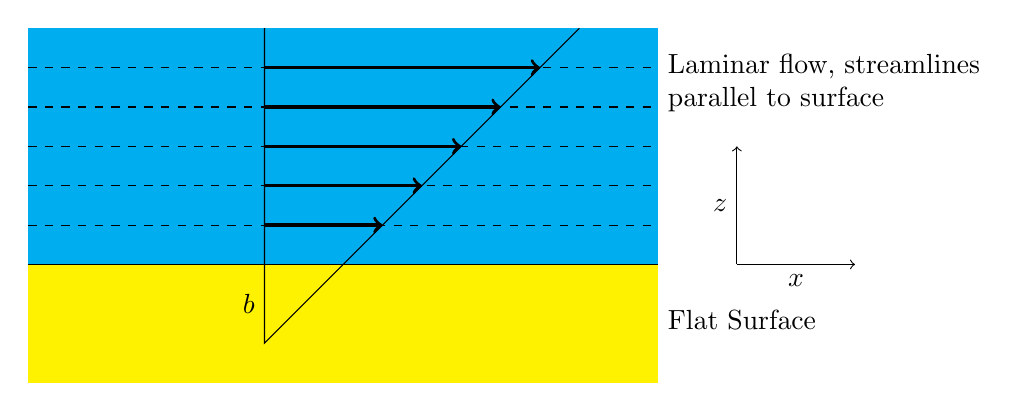
\begin{tikzpicture}
\fill[color=cyan] (-3,0) rectangle (5,3);
\fill [color=yellow] (-3,0) rectangle (5,-1.5);
\draw (-3,0) -- (5,0);
\foreach  \z in {0.5,1,...,2.5}
        {\draw[dashed] (-3,\z) -- ++(8,0);
         \draw[->, very thick](0,\z) -- ++(\z+1,0); };
\draw (0,3) -- (0,-1) -- ++(4,4);
\node at (0,-0.5)[left] {$b$};
\draw[->] (6,0) -- node[left] {$z$} ++(0,1.5);
\draw[->] (6,0) -- node[below] {$x$} ++(1.5,0);

\node at (5,-0.7)[right] {Flat Surface};
\renewcommand{\baselinestretch}{1.00}
\node at (5,2.3)[right,align=left]{Laminar flow, streamlines \\ parallel to surface};
%\node at (5,2.3) [right,align=left] {Laminar Flow,\\ with Streamlines\\Parallel to Surface};

\end{tikzpicture}
\caption{Simple shear.}\label{simpleshear}
\end{figure}

The laminae \emph{shear} past each other, giving rise to the viscous force.  The \emph{shear rate} is simply the velocity gradient: the rate of change of (parallel) velocity as we move in the normal direction.

The shear rate has an intuitive physical meaning.  Consider the action of simple shear on an infinitesimal cube of fluid: the cube starts with all sides at right angles, and is deformed into a parallelipiped.  The internal angle $\theta$ starts at $90^{\circ}$ and gets smaller.  In timeslice $\Delta t$ the change in angle $\Delta \theta$ causes the deformation shown in Figure (\ref{sheardeform}).

\clearpage
\begin{figure}[ht]
\centering
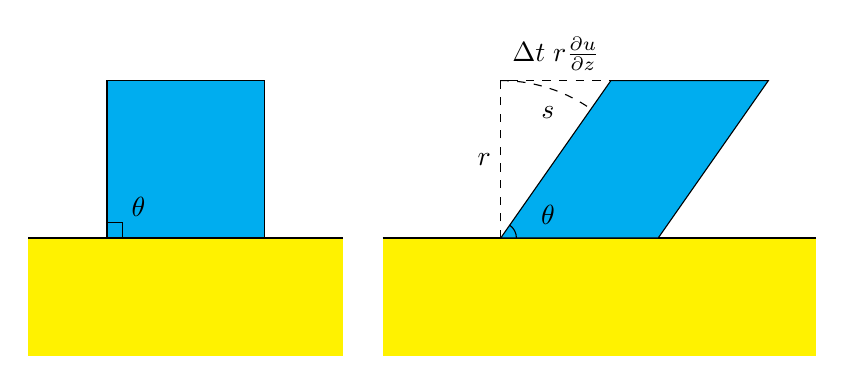
\begin{tikzpicture}

\fill[color=yellow] (-1,0) rectangle ++(4,-1.5);
\draw (-1,0) -- ++(4,0);
\draw[fill=cyan] (0,0) rectangle ++(2,2);
\draw (0.2,0) -- ++(0,0.2) -- ++(-0.2,0);
\node at (0.4,0.4) {$\theta $};


\fill[color=yellow] (3.5,0) rectangle ++(5.5,-1.5);
\draw (3.5,0) -- ++(5.5,0);
\draw[fill=cyan] (5,0) -- ++(1.4,2) -- ++(2,0) -- ++(-1.4,-2) -- ++(-2,0);

\draw[dashed] (5,0) -- node[left]{$r$} ++(0,2) -- node [above]{$\Delta t \; r \frac{\partial u}{\partial z}$} ++(1.4,0);
\draw[dashed] (5,2) arc (90:55:2cm);
\node at (5.6,1.6) {$s$};

\draw (5.2,0) arc (0:55:0.2cm);
\node at (5.6,0.3) {$ \theta$};

\end{tikzpicture}
\caption{Simple shear deforms an infinitesimal cube of fluid.}\label{sheardeform}
\end{figure}


In timeslice $\Delta t$, the top of the cube moves distance $\Delta t \, r \partial_z u$, and the angle changes by $\Delta \theta = s/r$.  For sufficiently small $\Delta t$, $s$ is much smaller than $r$, and $s \simeq \Delta t \, r \partial_y u$, so that $\Delta \theta \simeq \Delta t \, \partial_z u$.  In the limit $\Delta t \rightarrow 0$:

\begin{equation}
\text{shear rate} = \frac{d \theta}{d t} = \frac{\partial u}{\partial z}
\end{equation}


\subsection{Oblique Shear and the Velocity Gradient Tensor}
If the surface is still flat, but \textbf{not} oriented such that the surface maps nicely to the plane $z=0$, as in Figure (\ref{obliqueshear}), then the shear rate must be defined with vector derivatives.

\begin{figure}[ht]
\centering
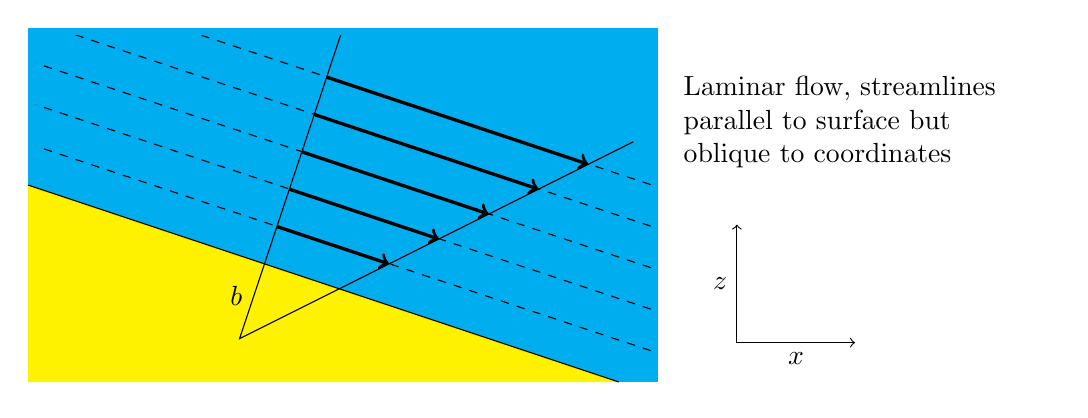
\begin{tikzpicture}
\fill[color=cyan] (-3,-1.5) rectangle (5,3);
\fill [color=yellow] (-3,-1.5) -- (-3,1) -- (4.5,-1.5);
\draw (-3,1) -- (4.5,-1.5);

\draw[->] (6,-1) -- node[left] {$z$} ++(0,1.5);
\draw[->] (6,-1) -- node[below] {$x$} ++(1.5,0);

%\node at (5,-0.7)[right] {Flat Surface};
%\node at (5.2,1.8) [right,align=left] {Laminar Flow,\\ with Streamlines\\Parallel to Surface,\\but oblique to\\coordinates};


\clip (-2.9,-1.6) rectangle ++(13,4.5);
\foreach  \z in {0.5,1,...,2.5}
        {\draw[dashed] (-3,\z*1.054 + 1) -- ++(8,-2.66);
         \draw[->, very thick](0.316*\z, 0.949* \z) --
          ++(0.949*\z + 0.949,- 0.316*\z - 0.316); };
\draw (1,3) -- (-.316,-0.949) -- ++(5,2.5);
\node at (-0.158,-0.4)[left] {$b$};

\renewcommand{\baselinestretch}{1.00}
\node at (5.2,1.8)[right,align=left] {Laminar flow, streamlines \\ parallel to surface but \\ oblique to coordinates};


\end{tikzpicture}
\caption{Oblique shear.}\label{obliqueshear}
\end{figure}

We introduce the unit vectors normal and tangent to the surface, $\vec{n}$ and $\vec{t}$. Then the tangential component of velocity is $ \vec{u} \cdot \vec{t}$.  
Because the streamlines are parallel to the flat surface, $\vec{u}$ is parallel to $\vec{t}$, so that $\vec{u} \cdot \vec{t}$ is in fact the \emph{magnitude} of $\vec{u}$.

We can define the shear rate as the rate of change of the tangential velocity in the normal direction. That is, the tangential component of the directional derivative of velocity in the normal direction.
The directional derivative of the velocity in the normal direction is $ \vec{n} \cdot \nabla \vec{u} $, and its tangential component is $ \vec{n} \cdot \nabla \vec{u} \cdot \vec{t}$.  See the schematic of Figure (\ref{flatshearrate}).

\begin{figure}[ht]
\centering
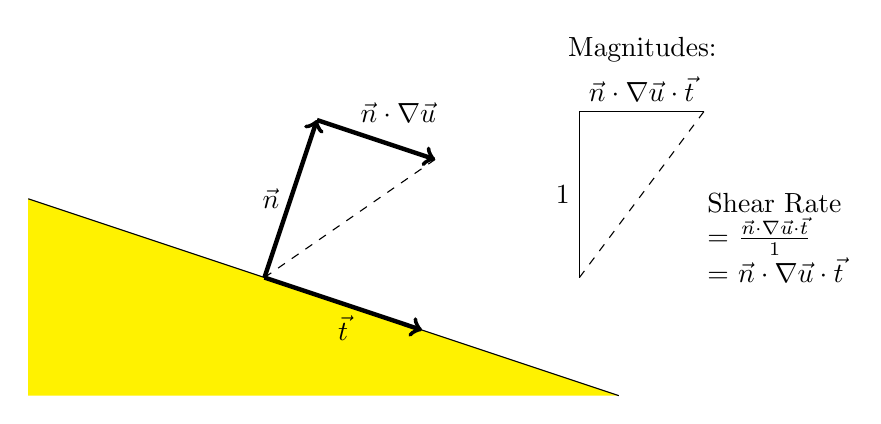
\begin{tikzpicture}
\fill[color=white] (-3,-1.5) rectangle (5,3);
\fill [color=yellow] (-3,-1.5) -- (-3,1) -- (4.5,-1.5);
\draw (-3,1) -- (4.5,-1.5);

%\draw[->] (6,-1) -- node[left] {$z$} ++(0,1.5);
%\draw[->] (6,-1) -- node[below] {$x$} ++(1.5,0);

\draw[ultra thick, ->] (0,0) -- node[left]{$\vec{n}$} (0.667,2);
\draw[ultra thick, ->] (0,0) -- node[below]{$\vec{t}$} (2,-0.667);

\draw[ultra thick, ->] (0.667,2) --  +(1.5,-0.5);
\node at (1.7,2.1) {$\vec{n} \cdot \nabla \vec{u}$};
\draw[dashed] (0,0) -- (2.167,1.5);

\draw (4,0) -- node[left]{1} ++(0,2.108) -- node[above]{$\vec{n} \cdot \nabla \vec{u} \cdot \vec{t}$} +(1.581,0);
\draw[dashed] (4,0) -- ++(1.581,2.108);

\node at (4.8,2.9) {Magnitudes:};
\node at (5.5,0.5)[right,align=left] {Shear Rate\\ = $\frac{\vec{n} \cdot \nabla \vec{u} \cdot \vec{t}}{1}$\\ = $ \vec{n} \cdot \nabla \vec{u} \cdot \vec{t}$};
\end{tikzpicture}
\caption{The shear rate at a flat surface of arbitrary orientation.}\label{flatshearrate}
\end{figure}

Thus for a \emph{flat} surface, with arbitrary coordinates, the shear rate is
\begin{equation}
\vec{n} \cdot \nabla \vec{u} \cdot \vec{t}
\end{equation}

%\clearpage Arbitrary 
\subsection{Curved Surface and Deformation Rate Tensor}



\begin{figure}[ht]
\centering
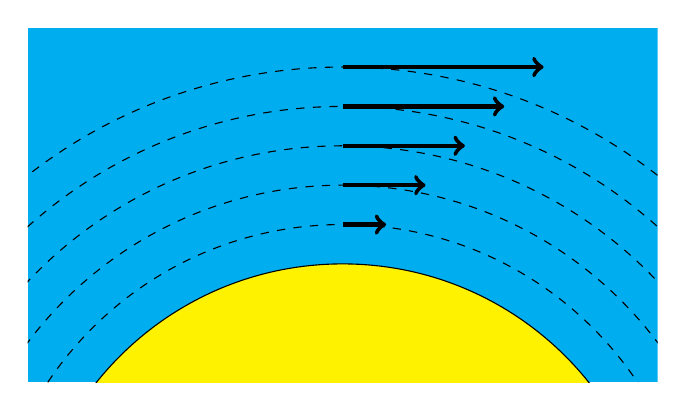
\begin{tikzpicture}
\clip (-4,-1.5) rectangle (4,3);
\fill[color=cyan] (-4,-1.5) rectangle (4,3);
\draw[fill=yellow] (0,-4) circle (4cm);

\foreach \k in {0.5cm,1cm,1.5cm,2cm,2.5cm}
           {
           \draw[dashed] (0,-4) circle (4cm + \k);
           \draw[ultra thick, ->] (0,\k) -- ++( 1.5 + \k,0);
           }



%\draw[fill=cyan] (0,0) rectangle ++(2,2);

\end{tikzpicture}
\caption{Laminar flow over a non-flat surface.}\label{nonflat}
\end{figure}

But what if the surface is not flat?  (Like Figure (\ref{nonflat}).)

It is tempting to assume the shear rate is the same as in the case of the generalized flat surface, as shown in the schematic of Figure (\ref{sameshear}).

\begin{figure}[ht]
\centering
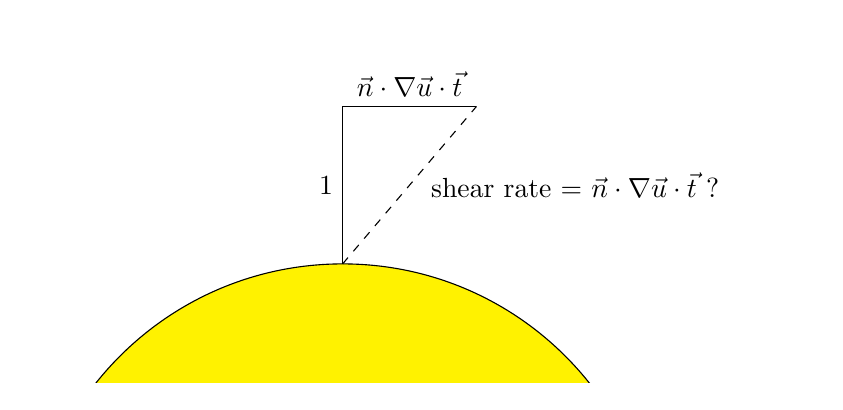
\begin{tikzpicture}
\clip (-4,-1.5) rectangle (6,3);

\draw[fill=yellow] (0,-4) circle (4cm);

\draw (0,0) -- node[left]{1}  ++(0,2) -- node[above] {$ \vec{n} \cdot \nabla \vec{u} \cdot \vec{t}$} ++(1.7,0);
\draw[dashed] (0,0) -- ++(1.7,2);

\node at (1,1)[right] {shear rate = $ \vec{n} \cdot \nabla \vec{u} \cdot \vec{t}$ ?};

\end{tikzpicture}
\caption{Is the shear rate the same as for a flat surface?}\label{sameshear}
\end{figure}

But consider the \emph{possible} action on an infinitesimal cube of fluid shown in Figure (\ref{cuberotates}).
\begin{figure}[ht]
\centering
\begin{tikzpicture}
\begin{scope}
    \clip (-2.5,-1.5) rectangle (2.5,3);

    \foreach \k in {0.5cm, 1cm, 1.5cm,2cm,2.5cm}
              {
              \draw[dashed] (0,-2.5) circle (2.5cm + \k);
              }
    \draw[fill=yellow] (0,-2.5) circle (2.5cm);
\end{scope}

\draw[fill=cyan] (0,0) rectangle ++(2,2);
\draw (0.2,0) |- (0,0.2);

\node at (0.2,0.4)[right] {$\theta = 90^{\circ}$};


\clip (3.2,-1.5) rectangle (8.5,3);

\foreach \k in {0.5cm, 1cm, 1.5cm,2cm,2.5cm}
              {
              \draw[dashed] (5.5,-2.5) circle (2.5cm + \k);
              }

\draw[fill=yellow] (5.5,-2.5) circle (2.5cm);
\draw[fill=cyan] (5.8,0) -- ++(0.5,2)-- ++(2,-0.5) --++(-0.5,-2) -- ++(-2,0.5);
\draw (5.8,0) -- ++(0.05,0.2) -- ++(0.2,-0.05) -- ++(-0.05,-0.2) -- ++(-0.2,0.05);

\node at (5.9,0.4)[right] {$\theta$ still $90^{\circ}$!};

\end{tikzpicture}
\caption{An infinitesimal cube may rotate without deforming.}\label{cuberotates}
\end{figure}

The infinitesimal cubical element has \emph{rotated} (and perhaps translated) but \emph{not deformed.}
The laminae have \emph{not} slid past each other, and the cube has not been subjected to shear.  There will be no viscous stress operating within the cube.

In this case, $ \vec{n} \cdot \nabla \vec{u} \cdot \vec{t}$ is not the shear rate of the cube, but the rate of rotation (angular velocity).  To get the true shear rate, we need to somehow remove the rotation.

The velocity gradient tensor (and Fr\'{e}chet derivative) \emph{linearize} the flow field. $\nabla \vec{u}$ is a linear transformation of a direction vector (the result being the correction vector).  Geometrically, a linear transformation can be decomposed into a rotation, an area-preserving deformation, and an expansion.  Following the exposition in the textbook \cite{Pozrikidis1997} of C. Pozrikidis:

\begin{equation}
\nabla \vec{u} = \mathbf{\Xi} + \mathbf{E} + \frac{1}{2} (\nabla \cdot \vec{u})  \mathbf{I}
\end{equation}

The rotation is represented in the \textbf{vorticity tensor}, $\mathbf{\Xi}$, the deformation in the \textbf{deformation rate tensor}, $\mathbf{E}$, and the expansion in $ \frac{1}{2} (\nabla \cdot \vec{u}) \mathbf{I}$

Working, for clarity, with 2-dimensional flow only, the vorticity tensor is:
\begin{equation}
\mathbf{\Xi} = \frac{1}{2}(\nabla \vec{u} - \nabla \vec{u}^T) = 
\frac{1}{2}
\begin{bmatrix}
0  & \partial_x v - \partial_y u \\
\partial_y u - \partial_x v  & 0
\end{bmatrix}
\end{equation}

The deformation rate tensor is:
\begin{equation}
\mathbf{E} = \frac{1}{2}(\nabla \vec{u} + \nabla \vec{u}^T) - \frac{1}{2}(\nabla \cdot \vec{u}) \mathbf{I} = 
\frac{1}{2} 
\begin{bmatrix}
\partial_x u - \partial_y v  & \partial_x v + \partial_y u  \\
\partial_y u + \partial_x v  & \partial_y v - \partial_x u
\end{bmatrix}
\end{equation}

The expansion rate tensor is:
\begin{equation}
\frac{1}{2}(\nabla \cdot \vec{u}) \mathbf{I} =
\frac{1}{2}
\begin{bmatrix}
\partial_x u + \partial_y v  &  0  \\
0  &  \partial_x u + \partial_y v
\end{bmatrix}
\end{equation}

We will deal with liquids, which we assume to be incompressible.  Thus the divergence vanishes:
\begin{equation}
\nabla \cdot \vec{u} = 0
\end{equation}
Therefore, the expansion term vanishes, and the deformation rate tensor simplifies to:
\begin{equation}
\mathbf{E} = \frac{1}{2}(\nabla \vec{u} + \nabla \vec{u}^T) = 
\frac{1}{2}
\begin{bmatrix}
2 \partial_x u   & \partial_x v + \partial_y u  \\
\partial_y u + \partial_x v  &  2 \partial_y v
\end{bmatrix}
\end{equation}

So for incompressible fluids, the linearized flow field is fully described by two terms, the \emph{antisymmetric} and \emph{symmetric} parts of the velocity gradient tensor:
\begin{equation}
\nabla \vec{u} =
\frac{1}{2}(\nabla \vec{u} - \nabla \vec{u}^T) +
\frac{1}{2}(\nabla \vec{u} + \nabla \vec{u}^T) 
 = \mathbf{\Xi} + \mathbf{E}
\end{equation}

We have solved our problem: removing the rotational transforms from the velocity gradient tensor is as simple as $\nabla \vec{u} - \mathbf{\Xi} = \mathbf{E}$.  So the deformation rate tensor $\mathbf{E}$ contains all transformations of the velocity gradient tensor \emph{other} than rotation.  Specifically, it must describe all shear.

We illustrate this in a simple example of 2-dimensional flow, where the normal and tangent vectors happen to align with the coordinate axes, as shown in Figure (\ref{shearrate}).

\begin{figure}[ht]
\centering
\begin{tikzpicture}
\everymath{\displaystyle}

\begin{scope}
    \clip (-2.5,-1.5) rectangle (2.5,1);
    \draw[fill=yellow] (0,-2.5) circle (2.5cm);
\end{scope}


\draw (0,0) -- node[left] {1} ++(0,2) -- node[above]{$\partial_y u $} ++(1,0);
\draw (0,0) -- node[below]{1} ++(2,0) -- node[right]{$\partial_x v$} ++(0,0.5);

\draw[color=red,ultra thick] (1,2)-- (0,0) -- (2,0.5);
\draw[dashed] (1,2) -- (0,0) -- (2,0.5);

\draw (0.4,0.1) arc (10:60:0.4cm);
\node at (0.5,0.4) {$\theta$};

\node at (2.2,1.7) [right] {$\frac{d\theta}{dt} = \partial_y u + \partial_x v$};

\draw[->] (-4,0) -- node[left] {$y$} ++(0,1.5);
\draw[->] (-4,0) -- node[below] {$x$} ++(1.5,0);

\end{tikzpicture}
\caption{The true shear rate at a point where the normal and tangent vectors align with the coordinate axes.}\label{shearrate}
\end{figure}

We see that the true shear rate at this point is $\partial_y u + \partial_x v$. The normal and tangent vectors at this point are:
\begin{equation}
\vec{n} = 
\begin{bmatrix}
0 \\ 1
\end{bmatrix}
, \quad
\vec{t} =
\begin{bmatrix}
1 \\ 0
\end{bmatrix}
, \quad
\end{equation}
 What is $\vec{n} \cdot 2 \mathbf{E} \cdot \vec{t}$ ?
\begin{equation}
\vec{n} \cdot 2 \mathbf{E} \cdot \vec{t} = 
\begin{bmatrix}
0 \\ 1
\end{bmatrix}
\cdot
\begin{bmatrix}
2 \partial_x u   & \partial_x v + \partial_y u  \\
\partial_y u + \partial_x v  &  2 \partial_y v
\end{bmatrix}
\begin{bmatrix}
1 \\ 0
\end{bmatrix}
=
\partial_y u + \partial_x v
\end{equation}


We have intuitively confirmed that for a general fluid flow, the shear rate associated with an infinitesimal plane is:
\begin{equation}
\text{shear rate} = \frac{d\theta}{dt} = \vec{n} \cdot 2 \mathbf{E} \cdot \vec{t}
\end{equation}
where $\vec{n}$ and $\vec{t}$ are the unit normal and tangent vectors to the plane.

\subsection{Generalized Slip Condition}

We have discovered the generalized shear rate: the rate of shear of an infinitesimal plane sliding over another infinitesimal plane.  If the plane is on the solid surface, then we can now write down a generalized Navier-type slip condition: the tangential velocity on the plane is proportional to the shear rate at the plane.  The constant of proportionality is of course the slip length $b$.

\begin{equation}
\vec{u} \cdot \vec{t} = b \; \vec{n} \cdot 2 \mathbf{E} \cdot \vec{t}
\end{equation}

Now $\mathbf{E}$ is symmetric, so $\vec{n} \cdot \mathbf{E} = \mathbf{E} \cdot \vec{n}$.  Furthermore, both sides of the equation are a dot product with $\vec{t}$, so we may simplify to:
\begin{equation}
\vec{u} = b \; 2 \mathbf{E} \cdot \vec{n}
\end{equation}

Or,
\begin{equation}
\vec{u} = b \, (\nabla \vec{u} + \nabla \vec{u}^T) \cdot \vec{n}
\label{eq:genslip}
\end{equation}


\vspace{1em}

It remains only to note that the slip length could be a \emph{function} of position on the boundary, and the boundary on which Equation (\ref{eq:genslip}) holds may also be described by a function. The boundary function will typically be a surface -- a `height' function $h(x,y)$ on the $x,y$ plane.


\subsection{Top Boundary Condition}

The simplest type of flow where an effective slip length is meaningful is Couette-like flow, driven by a constant velocity condition at the top of the bulk of fluid.  In a physical system, the constant velocity is provided by plate moving at a constant velocity in the $x$ direction only, located at some height $P$ above the slip surface.  The classic no-slip condition holds on the plate, so fluid at the top of the bulk has the same constant velocity.

In our model, at some height $P$ above the slip surface, there is a constant velocity $u_P$ in the $x$ direction only:
\begin{equation}
\vec{u}(x,y,P) = (u_P,0,0)
\end{equation}

(Incidentally, the homogenization procedure we employ in Chapter 6 does not actually need this top boundary condition, though the perturbation method used in Chapter 7 does.  This is a strength of the homogenization technique.)

\section{Complete Mathematical Model}

Our mathematical model can now be formally stated.  A bulk of fluid is situated above a boundary surface.  
The boundary surface is a function on the $x,y$ plane, and the $z$ direction is in general perpendicular to the boundary.

The fluid is an incompressible liquid, so the divergence is zero everywhere in the bulk:
\begin{equation}
\nabla \cdot \vec{u} = 0
\end{equation}

The liquid is Newtonian and the flow has a low Reynolds number, so flow at each point in the bulk obeys Stokes equation:
\begin{equation}
\mu \nabla^2 \vec{u} = \nabla p
\end{equation}
The velocity of the fluid at each point on the boundary satisfies the generalized slip boundary condition:
\begin{equation}
\vec{u} = b \, (\nabla \vec{u} + \nabla \vec{u}^T) \cdot \vec{n}
\end{equation}
At some height $P$ above the slip surface, there is a constant velocity $u_P$ in the $x$ direction only:
\begin{equation}
\vec{u}(x,y,P) = (u_P,0,0)
\end{equation}

\vspace*{3em}
In the next chapter we shall find an expression for the effective slip by finding a \textbf{homogenized} solution to these partial differential equations.

%\begin{center} \vspace{3em} \Coffeecup \end{center}

\iftoggle{compilealone}
    {
    \bibliography{Lund_Thesis.bib}
    \bibliographystyle{plain}
    }

\end{document}

TODO: clean up headings. Perhaps mention `directional derivative' and linearizing flow field in beginning.  Could also mention `vector gradient' and `tensor derivative' as meanings of $\nabla \vec{u}$, and `covariant derivative' as interpretation of $\nabla$.  But this seems unnecessary clutter.

 Maybe think about shear vector.  On second thoughts, no.  There is NO intuitive explanation of shear vector; I remember struggling with this 3 years ago.  Stress vector almost as bad.  Stress tensor is good for completeness, but unnecessary for this thesis. KISS.

\end{document}


%%%%%%%%%%%%%%%%%%%%%%%%%%%%%%%%%%%%%%%%%%%%%%%%%%%%%%%%%%%%%%%%%%%%%%%%%%%%%%%
%%%%%%%%%%%%%%   Old section introducing Navier Stokes equation.

\clearpage
\section*{Modeling the Bulk Fluid: Navier Stokes (Old)}

A fluid mechanics problem starts with a bulk of fluid.  At each point in the fluid, the fluid has a velocity, thus, the fluid bulk is modeled as a vector field in 3-D space, as shown in Figure (\ref{bulkfluid}).
%  In diagrams, representative vectors appear as arrows, with the length of the arrow proportional to the magnitude of the vector.

\begin{figure}[ht]
\centering
\begin{tikzpicture}

\fill[color=cyan] (0,0) rectangle (10,5);
\foreach \x in {1,2,3,4,5,6,7,8,9}
    \foreach \y in {1,2,3,4}
         \draw[->,thick](\x,\y) -- +(\y/5,0);

\end{tikzpicture}
\caption{A bulk of fluid with a velocity vector field.}\label{bulkfluidold}
\end{figure}


\subsection*{Incompressible Liquid}

For a vector field, a \textbf{flux} can be defined.  If the fluid is an incompressible liquid, then the flux into a volume element will exactly equal the flux out of the volume element.  This is expressed in the mathematical model by stating that the  divergence of the velocity vector field is zero everywhere:
\begin{equation}
\nabla \cdot \vec{u} = 0
\end{equation}
Incompressibility is a good approximation for liquids, and also turns out to be very mathematically convenient.
%This identity turns out to be extremely useful in making the ensuing mathematics tractable.



\subsection*{Viscous Newtonian Liquid, Old. Rewrite Below.}

An interesting fluid will also have other properties that hold at each point in the fluid: density $\rho$, pressure $p$, temperature.  Finally, fluids may have a \emph{viscosity} at each point, an `internal friction' that enables velocity to propagate through the fluid.  Viscosity is in fact the diffusion of momentum at the molecular level.
If the viscosity is constant throughout the fluid, and does not depend on velocity or velocity gradients, then the fluid is termed `Newtonian'. 

Viscosity acts with velocity gradients to produce \emph{forces} in the fluid. 
Consider an infinitesimal cubical volume element of fluid with velocity $\vec{u}$; for clarity, assume $\vec{u}$ points left-to-right.  Above the element is another fluid element which may have a different velocity.  The difference in velocities is approximately proportional to $\nabla \vec{u}$.  The viscous drag force on the original element is proportional to $\mu \nabla \vec{u}$, where $\mu$ is the coefficient of viscosity.   There is another fluid element below the original element, also causing a viscous drag force.   The \emph{net} viscous drag force on the original element is proportional to the rate of change of the velocity gradient, i.\ e.\ $ \mu \nabla^2 \vec{u}$.

The pressure $p$ is the force per unit area.  It acts on all faces of the fluid element and the \emph{net} force is proportional to the pressure gradient across the volume element, $\nabla p$.  The net pressure force combines with the net viscous force to form the net force on the fluid element.  The net force may cause the mass of the fluid element to accelerate in accordance with Newton's second law.  This law is embodied in the Navier-Stokes equation.


% An infinitesimal volume element in the fluid thus has a mass (density $\times$ volume) and experiences forces due to pressure and viscosity.  If we expect the laws of physics to hold in the fluid, then the volume element will obey Newton's second law $F= ma$.  This law is expressed as the Navier-Stokes equation.

If no body forces (eg. gravity) are relevant, and the fluid is \textbf{incompressible}, the Navier-Stokes equation is:

\begin{equation}
\rho \left( \frac{\partial \vec{u}}{\partial t} + (\vec{u}\cdot \nabla)\vec{u} \right) = -\nabla p +  \mu \nabla^2 \vec{u}
\end{equation}

If the equation is multiplied by the volume of the infinitesimal fluid element, then
the left-hand side is the acceleration, and the right-hand side is the force due to the pressure gradient and viscous shear.  The `advection operator'
 $(\vec{u} \cdot \nabla ) = u \partial_x + v \partial_y $
 gives the `inertial' term  $ (\vec{u}\cdot \nabla)\vec{u} $.


%%%%%%%%%%%%%%%%%%%%%%%%%%%%%%%%%%%%%%%%%%%%%%%%%%%%%%%%%%%%%%%%%%%%%%%%%%%%%%%%%%
% Cut out of section on magnitude of time-dependent velocity term.

%The characteristic time $T = L/U$ was chosen for dimensional convenience, not because it is a typical time scale.  It evaluates to
%\begin{equation}
%T = \frac{L}{U} = \frac{0.0001}{0.01} = 0.01 \;\; \text{seconds}
%\end{equation}
%
%Typically, for capillary flow experiments, velocity is constant, once equilibrium is reached. Thus, in general
%\begin{equation}
%\frac{\partial \hat{u}}{\partial \hat{t}} = 0
%\end{equation}
%In any case,  we can investigate how rapidly the velocity must change for this term to become significant:  If the characteristic velocity \emph{doubles}, and takes \emph{at least} 0.01 seconds to do so, then
%\begin{equation}
%\frac{\partial \hat{u}}{\partial \hat{t}} = \frac{1}{[\text{time} \geq 1]}\, \leq \, 1
%\end{equation}
%So if velocities in a microfluidic experiment change no quicker than doubling in 1/100th of a second, then the time-dependent term is at most of order one.  But typical capillary flow experiments involve steady flow, so this term vanishes.

% Finished July 18, 2013
% Put into format of VUW Thesis on March 20, 2014.

\documentclass[12pt, a4paper, twoside, openright]{book}

\usepackage{vuwthesis} % sets up some local things, mostly the front page

\setlength{\intextsep}{12pt} % set space above and below in-line float
\setlength{\abovecaptionskip}{0pt} % set space between figure and caption.


\usepackage{amssymb, amsmath}
%\usepackage{mathtools}
\usepackage{tikz}
\usetikzlibrary{calc}

\newcommand{\beff}{\ensuremath{b_{\mathrm{eff}}}}
\newcommand{\bhom}{\ensuremath{b_{\mathrm{hom}}}}
\newcommand{\bmin}{\ensuremath{b_{\mathrm{min}}}}


%\usepackage{marvosym}

\usepackage{etoolbox}
\newtoggle{compilealone}
\toggletrue{compilealone}

\title{Chapter 6: The Homogenized Effective Slip Length}
\author{Nat Lund}

\begin{document}
\chapter{The Homogenized Effective Slip Length}\label{C:homog}

In this chapter, we shall find the \emph{homogenized slip length} of a bulk of fluid flowing over a rough slippery surface.  We start by giving a high-level overview of the homogenization technique, then explain each aspect of homogenization in detail.  The first aspect we explain is the variational formulation and its relation to the calculus of variations.  Then the Stokes equations are put into variational form, then we find the variational formulation of the Stokes equation with the full tensor slip boundary condition.  We then take a step sideways and tackle the concept of weak convergence, and show that periodic functions weakly converge to their mean.  With all the machinery finally in place, we homogenize the variational formulation of the Stokes equation with tensor slip.  From the homogenized formulation, we derive the homogenized effective slip length.  We close the chapter with discussion of the physical interpretation of the result and its likely range of applicability.

\clearpage
In our mathematical model of the system, fluid flow at each point in the bulk obeys Stokes equation:
\begin{equation}
\mu \nabla^2 \vec{u} = \nabla p
\end{equation}
And fluid at each point on the boundary satisfies the generalized slip boundary condition:
\begin{equation}
\vec{u} = b \, (\nabla \vec{u} + \nabla \vec{u}^T) \cdot \vec{n}
\end{equation}

%The boundary itself roughly coincides with the $x,y$ plane. 
The boundary is a surface described by a periodic height function $h(x,y)$ on the $x,y$ plane.  $h(x,y)$ may be defined so that the $z=0$ plane is at the tops of the peaks of $h(x,y)$.  
%The $z$ direction is roughly perpendicular to the boundary, and 
The fluid may be supposed to be flowing in the $x$ direction. The model is summarized in Figure (\ref{homogmodel}).

\begin{figure}[ht]
\centering
\begin{tikzpicture}
\fill[color=cyan] (0,-1) rectangle (10,4);

\node at (5,2) {Bulk Condition: $\mu \nabla^2 \vec{u} = \nabla p$};
\node at (5,0.5){Boundary Slip Condition:  $\vec{u} = b \, (\nabla \vec{u} + \nabla \vec{u}^T) \cdot \vec{n}$};

\fill [color=yellow,domain=0:10,samples=200] plot (\x,{ 0.2 * sin(7*\x r)} ) -- ++(0,-2) -| (0,0);
\draw [domain=0:10,samples=200] plot (\x,{ 0.2 * sin(7*\x r)} );

\node at (5,-1) {Surface is Function $h(x,y)$};

\end{tikzpicture}
\caption{Summary of the mathematical model.}\label{homogmodel}
\end{figure}

The \emph{effective} slip length of a rough surface was defined back in Chapter 1.  At sufficient height above the surface, perturbations due to the rough surface have died away, and the flow \emph{behaves like} flow in an \emph{effective system:} flow over a flat `effective' surface with a uniform slip length, $\beff$. We illustrate this with Couette-type flow in Figure (\ref{Couettelike}).

\begin{figure}[ht]
\centering
\begin{tikzpicture}

\coordinate (ori) at (0,0);
%\fill[color=cyan] (ori) ++(0,-1) rectangle ++(4.5,5);
\fill [color=yellow,domain=0:4.5,samples=200] plot (\x,{ 0.2 * sin(7*\x r)} ) -- ++(0,-2) -| (ori);
\draw [domain=0:4.5,samples=200] plot (\x,{ 0.2 * sin(7*\x r)} );

\draw[dashed] (ori) ++(1.5,3.2) -- ++(0,-4.2) -- ++(3,4.5);
\draw[->, ultra thick] (ori) ++(1.5,2) -- ++(2,0);
\draw[->, ultra thick] (ori) ++(1.5,2.5) -- ++(2.33,0);
\draw[->, ultra thick] (ori) ++(1.5,3) -- ++(2.66,0);
\node at (2,0.7) {\Large{\textbf{?}}};
\node at (2.5,4) {Smooth Couette flow in far field};


\coordinate (ori) at (6,0);
%\fill[color=cyan] (ori) ++(0,-1) rectangle ++(4.5,5);
\fill[color=yellow] (ori) rectangle ++(4.5,-2);
\draw (ori) -- ++(4.5,0);

\draw[dashed] (ori) ++(1.5,0) -- ++(0,-1) -- ++(3,4.5);
\draw[<->] (ori) ++(1.3,0) -- node[left] {\beff} ++(0,-1);

\draw[<-] (4.15,2.7) -- ++(1.3,0.4);
\draw[<-] (9.8,2.7) -- ++(-1.3,0.4);
\node at (7,3) [align=center] {Same flow profile\\$u = \dot{\gamma} (z + \beff)$};

\node at (2.5,5) {\textsc{physical system}};
\node at (8.25,5) {\textsc{effective system}};


\end{tikzpicture}
\caption{The effective slip length of Couette-type flow.}\label{Couettelike}
\end{figure}


\subsection{Homogenization}

Homogenization is a modern technique for approximating the solutions of partial differential equations, developed in the 1960s and '70s.  It began with the study of PDEs with rapidly oscillating coefficients.  
The basic idea was to identify the period of oscillation with a small parameter $\epsilon$, and to consider the limit as the period tended to zero.  Depending on the problem, one may get a solution as a series in $\epsilon$: $u = u_0 + \epsilon u_1 + \cdots$, or one may obtain a limiting PDE for which a solution can be found.
The technique can be applied to PDEs that hold on periodic structure; $\epsilon$ is the period of the structure.  Then we find an `effective' structure as the period of the structure tends to zero.  The first book describing homogenization appeared in 1978: ``Asymptotic Analysis for Periodic Structure", by Alain Bensoussan, Jacques-Louis Lions and George Papanicolaou.  

In standard homogenization techniques, it turns out to be necessary to cast the differential equations into variational or integral form.  As a consequence, in some cases it may be possible to exploit the fact that periodic functions weakly converge to their average.  (Weak convergence --- a `convergence under the integral sign' --- will be defined shortly.)
The homogenized solution is an approximation to the solution for a system with a finite period.  The smaller the period, the better the approximation.



\vspace{1em}
Thus, homogenization is perfectly suited to our task.  
In order to use homogenization, we must slightly extend our mathematical model with the following assumptions:

\vspace{1em}
First of all, we must assume that our surface roughness is \textbf{periodic}.  That is, $h(x,y)$ is a periodic function.  This is reasonable, many real rough surfaces are at least quasi-periodic; there seems no loss of information by assuming that the surface is periodic.

Secondly, we must assume the the intrinsic slip length is a periodic function with the \textbf{same period as the roughness}. % Again, this is reasonable.   
This is applicable in many situations -- though there may be interesting exceptions -- since
in many physical systems, the change in intrinsic slip length is \emph{due to} the roughness, eg. the increased slip over nanobubbles.

\vspace{1em}
Then, broadly speaking, the homogenization procedure is as follows:
The period is reduced sequentially, eg. the period is halved at each step in a sequence.
The \emph{amplitude} of the roughness must be reduced at the same rate, so that local gradient and curvature of the surface remain unchanged.  In the limit of the period tending to zero, we have the \textbf{homogenized} equations of flow, which we can consider to model a homogenized system.  The homogenized equations contain a slip length parameter.  In the language of homogenization theory, this is known as the \textbf{effective} slip length parameter.
We  illustrate this with Couette-type flow in Figure (\ref{Couettehomog}).

\begin{figure}[ht]
\centering
\begin{tikzpicture}

\coordinate (ori) at (0,0);
%\fill[color=cyan] (ori) ++(0,-1) rectangle ++(4.5,5);
\fill [color=yellow,domain=0:4.5,samples=200] plot (\x,{ 0.2 * sin(7*\x r)} ) -- ++(0,-2) -| (ori);
\draw [domain=0:4.5,samples=200] plot (\x,{ 0.2 * sin(7*\x r)} );

\draw[dashed] (ori) ++(1.5,3.2) -- ++(0,-4.2) -- ++(3,4.5);
\draw[->, ultra thick] (ori) ++(1.5,2) -- ++(2,0);
\draw[->, ultra thick] (ori) ++(1.5,2.5) -- ++(2.33,0);
\draw[->, ultra thick] (ori) ++(1.5,3) -- ++(2.66,0);
\node at (2,0.7) {\Large{\textbf{?}}};
\node at (3.2,-0.8)[align=center] {Periodic\\ Surface};


\coordinate (ori) at (6,0);
%\fill[color=cyan] (ori) ++(0,-1) rectangle ++(4.5,5);
\fill[color=yellow] (ori) rectangle ++(4.5,-2);
\draw (ori) -- ++(4.5,0);

\draw[dashed] (ori) ++(1.5,0) -- ++(0,-1) -- ++(3,4.5);
\draw[<->] (ori) ++(1.3,0) -- node[left] {\beff} ++(0,-1);

\draw[<-] (9.8,2.7) -- ++(-0.7,0.3);
\node at (8,3) [align=center] {Homogenized\\ flow profile\\$u = \dot{\gamma}( z + \beff)$};

\node at (2.5,5) {\textsc{physical system}};
\node at (8.25,5) {\textsc{homogenized system}};

\fill (5.8,0) -- ++(-0.2,0.2) -- ++(0,-0.1) --++(-0.9,0) -- ++(0,-0.2) -- ++(0.9,0) -- ++(0,-0.1);

\end{tikzpicture}
\caption{The homogenized effective slip length of Couette-type flow.}\label{Couettehomog}
\end{figure}

For Couette-type flow, we have defined the effective slip length as the slip length of an `effective' physical system, with flow solution $u = \dot{\gamma} (z + \beff)$.

If the same system is homogenized, the solution to the homogenized equations is $u = \dot{\gamma} (z + \beff)$.  We see immediately that the homogenized effective slip length exactly matches our physical definition of effective slip length.

\vspace{1em}
Let us now homogenize the Stokes equations for flow over rough periodic surfaces with variations in slip of the same period.  The particular homogenization technique we shall use comprises the following steps:

\subsubsection{Homogenization Process Overview}

\begin{enumerate}
\item Convert the model PDEs to variational (integral) form.
\item Create a sequence of variational formulations.
\item Find the limit formulation of the sequence:
\begin{itemize}
    \item Periodic functions weakly converge to their mean;
    \item This lets us find the limit formulation.
\end{itemize}
      
\item Convert the limit formulation back to classical formulation
\item Extract the implied slip length as the \emph{homogenized} slip length.
\end{enumerate}



\section{Variational Form}

The variational form comes originally from the Calculus of Variations.  The canonical use for the calculus of variations is with a \emph{minimization} problem.  We seek a \emph{function} on a domain that minimizes some quantity.  The quantity to be minimized is a \emph{functional}, a mapping from the space of functions to the real numbers.  The functional will be some kind of integral, with the integrand being some combination of the function, its derivatives (of various order), and position in the domain.

\begin{equation}
F(u) = \int_a^b f(u,u', ...\, ,x) \; dx,  \qquad F(u) \mapsto \mathbb{R}
\end{equation} 

The boundary values of the function $u(x)$ are given.  The basic concept of calculus of variations is to take $u(x)$ to be the solution function that minimizes the functional $F$.  That being the case, any \emph{variation} away from $u$, however small, will increase $F$.  Let $v(x)$ be an arbitrary function that is zero at the boundary (i.e. zero at $a$ and $b$), and let $\epsilon$ be a small parameter. Then:
\begin{equation}
F(u) \leq F(u + \epsilon v) \qquad \forall v: v(a) = v(b) = 0
\end{equation}
This minimizing function and variation are depicted in Figure (\ref{variation_c}).

\begin{figure}[ht]
\centering
\begin{tikzpicture}

\draw[<->] (7,0) -- (0,0) -- node[left]{$u(x)$} (0,5);
\node at (6.5,0) [below] {$x$};
\draw[dotted] (1,0) -- +(0,3);
\draw[dotted] (5,0) -- +(0,4.5);
\node at (1,0)[below] {$a$};
\node at (5,0)[below] {$b$};

%\draw[very thick] (1,2) to [out=-50, in=180] (2,1.5) to [out=0,in=240] (5,3.5);
\draw[very thick, domain=1:5] plot (\x, { 1.5 + 0.25*(\x-2)*(\x-2) });
\draw[color=red,thick, samples=97, domain=1:5] plot (\x, { 0.2 * sin( 3*pi*(\x-1) r) } );
\draw[color=red,thick, samples=97, domain=1:5] plot (\x, { 1.5 + 0.25*(\x-2)*(\x-2) + 0.2 * sin( 3*pi*(\x-1) r)  });

\draw[<-](4.7,0.3) -- (5.5,1);
\node at (5.5,1.1)[right] {variation $v$};
\draw[<-] (4.62,3.05) -- (5.5,2.7);
\node at (5.5,2.7)[right] {$u$};
\draw[<-] (4.3,2.5) -- (5.5,2);
\node at (5.5,2)[right] {$u + \epsilon v$};

\end{tikzpicture}
\caption{The minimizing function $u(x)$ and an arbitrary variation $v(x)$ added to it.}\label{variation_c}
\end{figure}

For an arbitrary variation $v$, the small parameter $\epsilon$ can be treated as a variable, so that $F(u + \epsilon v)$ is a function from $\mathbb{R}$ to $\mathbb{R}$. Since $u$ minimizes $F$, $\epsilon = 0$ minimizes $F(\epsilon): \mathbb{R} \mapsto \mathbb{R}$. % Here's the cunning bit: 
The minimum is a stationary point, so the \emph{slope} of $F(\epsilon)$ is zero also at the minimum.  That is, for minimizing function $u$, for any variation $v$,

\begin{equation}
\frac{d}{d \epsilon} F(u + \epsilon v) = 0
\end{equation}
This is shown in Figure (\ref{minimum_c}).

\begin{figure}[ht]
\centering
\begin{tikzpicture}
\draw[<->] ( -3,0) -- (3,0);
\draw[->] (0,0) --  (0,3);
\node at (2,0) [below] {$\epsilon$};
\node at (0,0) [below] {0};
\node at (0,2.5)[right]{$F(u + \epsilon v) $};

%\draw[thick,dashed] (-2.5,3) to [out=-60, in=180] (0,1) to [out=0, in=240] (2.5,3);
\draw[thick, domain=-2.5:2.5] plot ( \x, {1 + 0.3* \x*\x} );

\draw[dashed] (-1,1) -- +(2,0);
\node at (0,0.6) [right] {$\frac{d}{d \epsilon} F(u + \epsilon v) = 0$};
 
\end{tikzpicture}
\caption{The slope of $F(\epsilon)$ is zero at the minimum of $F(\epsilon)$.}\label{minimum_c}
\end{figure}


\subsection{Example: Energy Balance}

The fully-worked standard example of energy balance appears in Appendix D.  We give a summary here.

Consider a film of soapy water suspended across an aperture.  At equilibrium, the soap film lies in the $x,y$ plane.  Let $u(x,y)$ be the the height of the film above the $x,y$ plane (at point ($x,y$)), as in the schematic of Figure (\ref{soapy_c}).

\begin{figure}[ht]
\centering
\begin{tikzpicture}

\draw [thick] (0,0) arc (120:60:7cm);
\draw (0,0) arc (120:60:7cm) [dashed] -- (0,0);

\draw [fill=gray] (0,0) rectangle ++(-1,-0.5);
\draw [fill=gray] (7,0) rectangle ++(1,-0.5);

\draw[->] (3,0) -- node[right]{$u(x,y)$} ++(0,0.92);

\end{tikzpicture}
\caption{A film of soapy water suspended across an aperture.}\label{soapy_c}
\end{figure}

\clearpage
Assume a pressure below the film distorts it, pushing it upwards.  If $f$ is the pressure, then the pressure force does work on the film equal to: $ W = \int_{\Omega} f u \,dA $.  The work done on the soap film is stored as elastic potential energy.  The soap film has a constant surface tension $k$ that acts tangentially to the surface.  The change in potential energy is proportional to the change in surface area, specifically $ U = k \frac{1}{2} \int_{\Omega} |\nabla u|^2 \;dA $.
A summary schematic is shown in Figure (\ref{balance_c}).

\begin{figure}[ht]
\centering
\begin{tikzpicture}

\draw [fill=cyan] (0,0) arc (120:60:7cm) [dashed] -- (0,0);
\draw [thick] (0,0) arc (120:60:7cm);

\draw [fill=gray] (0,0) rectangle ++(-1,-0.5);
\draw [fill=gray] (7,0) rectangle ++(1,-0.5);

\draw[<-] (3,0) -- node[right]{pressure $f(x,y)$} ++(0,-0.7);
\draw[<-] (1,0) -- ++(0,-0.7);
\draw[<-] (2,0) -- ++(0,-0.7);

\draw[<-] (4,0.5) -- ++(0.8,2.2);
\node at (6,3) {$\displaystyle W = \int_{\Omega} f u \,dA $};

\draw[<-] (2.5,0.9) -- ++(-0.7,1.5);
\node at (1.5,3) {$\displaystyle U = k \frac{1}{2} \int_{\Omega}  |\nabla u|^2 \;dA  $};

\renewcommand{\baselinestretch}{1.00}
\node at (-0.5,1)[align=center] {Increase in surface\\ area $ \frac{1}{2} \int_{\Omega}  |\nabla u|^2 \;dA $ };

\end{tikzpicture}
\caption{The work done distorting the soap film is equal to the elastic potential energy due to the increase in area.}\label{balance_c}
\end{figure}

%\textbf{NOTE:}  This also models the energy balance of a deformed rubber membrane, \emph{if} the deformation is small enough that the tension is considered to be \emph{constant} throughout the deformation (rather than increasing linearly with area).
The elastic potential energy is exactly equal to the work done on the soap film by the pressure:
\begin{equation}
k \frac{1}{2} \int_{\Omega} |\nabla u|^2 \;dA = \int_{\Omega} f u \;dA
\end{equation}
We can express this as a functional to be minimized:
\begin{equation}
F(u) =  k \frac{1}{2} \int_{\Omega} |\nabla u|^2 \,dA - \int_{\Omega} f u \,dA
\end{equation}
And take the functional derivative:                  
\begin{align}
\frac{d}{d\epsilon}F & = \lim_{\epsilon \rightarrow 0}
                         \frac{F(u + \epsilon v) - F(u)}{\epsilon} \\
  & =
    k \int_{\Omega} \nabla u \cdot \nabla v \,dA
        - \int_{\Omega} f v \,dA     
\end{align}
Thus the variational form $\frac{d}{d\epsilon}F = 0$ is:
\begin{equation}
k \int_{\Omega} \nabla u \cdot \nabla v \,dA
        - \int_{\Omega} f v \,dA = 0
\end{equation}
This relation is true for any \emph{almost} arbitrary variation $v$.  In fact, $v$ must be integrable on the domain $\Omega$, and its first derivatives must be integrable on $\Omega$.
The space of functions meeting these requirements is known as the Sobolev space $H^1(\Omega) $.  So formally, $v$ belongs to the Sobolev space:
\begin{equation}
v \in H^1 (\Omega)
\end{equation}
Moreover, because the value of $u$ is given at the boundary, $v$ must be zero at the boundary.  Formally, $v$ is in the Sobolev space:
\begin{equation}
v \in H_0^1 (\Omega)
\end{equation}

\section{Alternative Route to Variational Form}

The point is that the variational form
\begin{equation}
k \int_{\Omega} \nabla u \cdot \nabla v \,dA  - \int_{\Omega} f v \,dA = 0
\qquad
\forall v \in H_0^1(\Omega)
\end{equation}
may be easier to solve than the original energy functional:
\begin{equation}
k \frac{1}{2} \int_{\Omega} |\nabla u|^2 \,dA - \int_{\Omega} f u \,dA = 0
\end{equation}
However, the variational form can be derived by other means.  In fact, there are variational formulations for which there is \emph{no} corresponding functional to minimize.  So in a sense the variational formulation is more fundamental than the calculus of variations.

To illustrate:  The functional $ \frac{1}{2} \int_{\Omega} |\nabla u|^2 \,dA $ 
is known as Dirichlet's energy functional.  A solution $u$ that minimizes the functional is \emph{also} a solution to the Laplace equation $ \nabla^2 u = 0 $.
This energy functional can be put into the variational form $ \int_{\Omega} \nabla u \cdot \nabla v \,dA $ by using the calculus of variations.  However, the variational form $ \int_{\Omega} \nabla u \cdot \nabla v \,dA $ can also be derived directly from the Laplace equation.
\begin{equation}
u \; \text{minimizing} \;\;\; \frac{1}{2} \int_{\Omega} |\nabla u|^2 \,dA
\;\;\; \text{also satisfies} \;\; \int_{\Omega} \nabla u \cdot \nabla v \,dA = 0
\;\;\; \text{iff} \;\;\; \nabla^2 u =0 
\end{equation}

We shall use this alternative derivation as part of our homogenization procedure.
We bootstrap by building up from simpler cases:  First, we derive the variational form $ - \int_{\Omega} \nabla u \cdot \nabla g \,dA = \int_{\Omega} g f \,dA $ directly from the Poisson equation $ \nabla^2 u = f$, which we can think of as the $x$ velocity equation of Stokes flow with the pressure gradient given as (scalar) $f$.

Note on notation:  In an integral such as $ \int_{\Omega} g f \,dA $, the integration measure $dA$ is implied by the subscript $\Omega$ denoting integration over the domain.  Therefore, to improve readability -- without loss of clarity -- we shall usually drop the integration measures (such as $dA$) from the integrals.

\subsection{Variational Form of Poisson Equation inspired by Stokes Flow}

Here we derive the variational form $ - \int_{\Omega} \nabla u \cdot \nabla g = \int_{\Omega} g f $ directly from the Poisson equation $ \nabla^2 u = f$.  This is the $x$ velocity equation of Stokes flow with the pressure gradient given as scalar $f$, and the no-slip boundary condition.

Before beginning, we recall a vector identity.  For scalars $g$ and $u$:
% "Too much detail.  Your examiners can do this in their heads..."
%\begin{align*}
%g \nabla^2 u & = g \partial_x^2 u + g \partial_y^2 u \\
%\nabla u \cdot \nabla g & = \partial_x u \partial_x g + \partial_y u \partial_y g \\
%\nabla \cdot (g \nabla u) & = \partial_x (g \partial_x u) + \partial_y (g \partial_y u) \\
%  & = \partial_x u \partial_x g + g \partial_x^2 u + \partial_y u \partial_y g + g \partial_y^2 u \\ 
%  & = \nabla u \cdot \nabla g + g \nabla^2 u 
%\end{align*}
\begin{equation}
%\therefore \quad 
g \nabla^2 u = \nabla \cdot (g \nabla u) - \nabla u \cdot \nabla g
\end{equation}

\vspace{2em}

On some domain $\Omega$, as in Figure (\ref{domain}), the Poisson equation holds:
\begin{equation}
\nabla^2 u = f \qquad \text{on} \; \Omega
\end{equation}

\vspace{1em}
\begin{figure}[ht]
\centering
\begin{tikzpicture}
\draw[dashed] (0,0) rectangle (4,2);

\node at (2,1) {$\Omega $};
\node at (4.5,1) {$\Gamma $};
\end{tikzpicture}
\caption{A domain $\Omega$ with boundary $\Gamma$.}\label{domain}
\end{figure}

\clearpage
We introduce a \emph{test function} $g$, from the appropriate Sobolev space:  $g$ and its first derivatives are integrable on $\Omega$, and $g$ is zero on the boundary $\Gamma$:
\begin{equation}
g \in H_0^1(\Omega) \qquad (g=0 \; \text{on} \; \Gamma)
\end{equation}

We multiply the Poisson equation by the test function $g$:
\begin{equation}
g \nabla^2 u = g f
\end{equation}
and integrate over the domain $\Omega$:
\begin{equation}
\int_{\Omega} g \nabla^2 u = \int_{\Omega} g f
\end{equation}
then substitute $g \nabla^2 u = \nabla \cdot (g \nabla u) - \nabla u \cdot \nabla g$:
%\begin{equation}
%\int_{\Omega} \nabla \cdot (g \nabla u) - \nabla u \cdot \nabla g  
%= \int_{\Omega} g \nabla p
%\end{equation}
\begin{equation}
\int_{\Omega} \nabla \cdot (g \nabla u) - \int_{\Omega} \nabla u \cdot \nabla g  
= \int_{\Omega} g f
\label{eq:poissint}
\end{equation}

\begin{equation}
\text{Recall the Divergence Theorem:} \qquad
\int_{\Omega} \nabla \cdot \vec{a}  = \int_{\Gamma} \vec{a} \cdot \vec{n}
\end{equation}
Therefore the first term of Eq. (\ref{eq:poissint}) is:
\begin{equation}
\int_{\Omega} \nabla \cdot (g \nabla u) = 
\int_{\Gamma} (g \nabla u) \cdot \vec{n} = \int_{\Gamma} g (\nabla u \cdot \vec{n})
= \int_{\Gamma} g \frac{\partial u}{\partial n}
\end{equation}
Now the test function $g$ was defined to be zero on $\Gamma$, thus
\begin{equation}
\int_{\Omega} \nabla \cdot (g \nabla u)
 = \int_{\Gamma} g \frac{\partial u}{\partial n} =0
\end{equation}

This leaves finally:
\begin{equation}
- \int_{\Omega} \nabla u \cdot \nabla g  
= \int_{\Omega} g f
\end{equation}
which closely resembles the variational form derived from the energy functional.


\subsection{Variational Form of Poisson Equation inspired by Stokes Flow with Slip}

We now progress to the variational form of the Poisson equation inspired by Stokes flow over a flat boundary with Navier slip.

On the domain $\Omega$, the Poisson equation holds:
\begin{equation}
\nabla^2 u = f \qquad \text{on} \; \Omega
\end{equation}

Now the boundary of the entire domain, $\Gamma$, must be split up into the \emph{bottom} boundary $\Gamma_b$, and the rest of the boundary, $\Gamma_0$, as shown in Figure (\ref{splitboundary}).  The bottom boundary $\Gamma_b$ is the solid surface with slip.  The boundary condition on $\Gamma_b$ has the form of Navier slip:
\begin{equation}
u = b \frac{\partial u}{\partial n} \qquad \text{on} \; \Gamma_b
\end{equation}

\vspace{1em}
\begin{figure}[ht]
\centering
\begin{tikzpicture}
\draw (0,0) -- (4,0);
\draw[dashed] (0,0) -- ++(0,2) -| (4,0);

\node at (2,1) {$\Omega $};
\node at (2,-0.5) {$\Gamma_b$};
\node at (4.5,1) {$\Gamma_0 $};
\end{tikzpicture}
\caption{Domain $\Omega$ with slip boundary $\Gamma_b $ and remainder of boundary $\Gamma_0 $.}\label{splitboundary}
\end{figure}


Now care must be taken to choose the appropriate function space for our test function.  As before, the  test function and its first derivatives must be integrable on $\Omega$.  
But now, $g$ must vanish on all of the boundary \emph{except} the bottom boundary $\Gamma_b$:

\begin{equation}
g \in H^1_{\Gamma_b} (\Omega) = \lbrace g \in H^1(\Omega): g = 0 \; \text{on}\; \Gamma_0 \rbrace 
\quad (g \neq 0 \; \text{on} \; \Gamma_b)
\end{equation}

Multiply  by $g$ and integrate over $\Omega$:
\begin{equation}
\int_{\Omega} g \nabla^2 u = \int_{\Omega} g f
\end{equation}

Ending up with
\begin{equation}
\int_{\Gamma} g \frac{\partial u}{\partial n}
 - \int_{\Omega} \nabla u \cdot \nabla g  
= \int_{\Omega} g f
\end{equation}
Now, $g=0$ on all of $\Gamma$ except the bottom boundary, so:
\begin{equation}
\int_{\Gamma} g \frac{\partial u}{\partial n}
= \int_{\Gamma_b} g \frac{\partial u}{\partial n}
\end{equation}
The slip condition on $\Gamma_b$ implies:
\begin{equation}
\frac{\partial u}{\partial n} = \frac{1}{b}u
\end{equation}
So we substitute this, to get our variational form:
\begin{equation}
\int_{\Gamma_b} g \frac{1}{b} u 
 - \int_{\Omega} \nabla u \cdot \nabla g  
= \int_{\Omega} g f
\end{equation}

\clearpage
\section{Variational Form of Stokes Flow with\\ Tensor Slip}

\subsection{Tensor Identities}

Before deriving the variational formulation of our full model of 3-D flow with tensorial slip, we define the tensor double dot product and recall a tensor identity.

\subsubsection{Tensor Double Dot Product}

The double dot product of two tensors, also known as the Frobenius inner product, is a generalization of the vector inner product:

\begin{equation}
A = 
\begin{bmatrix}
a & b \\
c & d
\end{bmatrix}
, \quad Z = 
\begin{bmatrix}
x & y \\
z & w
\end{bmatrix}
, \quad
A:Z = ax + by + cz + dw
\end{equation}

\subsubsection{Tensor Identity with Deformation Rate Tensor}

In Appendix E, we prove the following identity:
\begin{equation}
\nabla^2 \vec{u} \cdot \vec{g} = 
\nabla \cdot ( (\nabla \vec{u} + \nabla \vec{u}^T) \cdot \vec{g})
- 2 \mathbf{E}(\vec{u}):\mathbf{E}(\vec{g})
\label{tensoridentity}
\end{equation}
This identity assumes $\nabla \cdot \vec{u} = 0$.

\clearpage
\subsection{Variational Form of Stokes Flow with Tensor Slip}

We have a domain $\Omega$, the boundary of which is made up of two parts, $\Gamma_b$ and $\Gamma_0$, as shown in Figure (\ref{Stokesdomain}).  On the domain $\Omega$ we have incompressible Stokes flow:
\begin{gather}
\nabla^2 \vec{u} = \frac{1}{\mu} \nabla p  \\
\nabla \cdot \vec{u} = 0
\end{gather}
On the rough boundary $\Gamma_b$ we have the tensor slip condition:
\begin{equation}
\frac{1}{b} \vec{u} = (\nabla \vec{u} + \nabla \vec{u}^T)\cdot \vec{n}
\quad \text{or} \quad
\frac{1}{b} \vec{u} = 2 \mathbf{E}(\vec{u}) \cdot \vec{n}
\label{tensorslipBC}
\end{equation}

\begin{figure}[ht]
\centering
\begin{tikzpicture}

\draw [domain=0:4.5,samples=200] plot (\x,{ 0.2 * sin(7*\x r)} );
\draw[dashed] (0,0) -- ++(0,2) -| (4.5,0);

\node at (2.25,-0.5) {$\Gamma_b $};
\node at (5,1) {$\Gamma_0 $};
\node at (2.25,1) {$\Omega $};

\end{tikzpicture}
\caption{Domain $\Omega$ with rough slip boundary $ \Gamma_b $ and remainder of boundary $\Gamma_0$.}\label{Stokesdomain}
\end{figure}

We introduce an arbitrary test function $\vec{g}$ from the appropriate Sobolev space:
\begin{equation}
\vec{g} \in H^1_{\Gamma_b}(\Omega) = 
\{ \vec{g} \in H^1(\Omega), \quad \nabla \cdot \vec{g} = 0 \text{ in } \Omega ,
 \quad \vec{g}=0 \text{ on } \Gamma_0 \}
\end{equation}

We take the dot product of the Stokes PDE with $\vec{g}$:
\begin{equation}
\nabla^2 \vec{u} \cdot \vec{g} = \frac{1}{\mu} \nabla p \cdot \vec{g}
\end{equation}
and integrate over the domain:
\begin{equation}
\int_{\Omega} \nabla^2 \vec{u} \cdot \vec{g} = 
\frac{1}{\mu} \int_{\Omega}  \nabla p \cdot \vec{g}
\end{equation}

%%%%
%Consider the right hand side.  Recall that by integration by parts:
%\begin{equation}
%\frac{1}{\mu} \int_{\Omega}  \nabla p \cdot \vec{g} = 
%\frac{1}{\mu} \int_{\Omega} \nabla \cdot p\vec{g} - 
%\frac{1}{\mu} \int_{\Omega} p \nabla \cdot \vec{g}
%\end{equation}
%By the Divergence Theorem:
%\begin{equation}
%\frac{1}{\mu} \int_{\Omega} \nabla \cdot p\vec{g} =
%\frac{1}{\mu} \int_{\Gamma} p \vec{g} \cdot \vec{n} =
%\frac{1}{\mu} \int_{\Gamma_b} p \vec{g} \cdot \vec{n} +
%\frac{1}{\mu} \int_{\Gamma_0} p \vec{g} \cdot \vec{n}
%\end{equation}


%Thus we have
%\begin{equation}
%\int_{\Omega} \nabla^2 \vec{u} \cdot \vec{g} = 
%\frac{1}{\mu} \int_{\Omega}  \nabla p \cdot \vec{g}
%\end{equation}

Substitute  $ \nabla^2 \vec{u} \cdot \vec{g} = \nabla \cdot ( 2 \mathbf{E}(\vec{u}) \cdot \vec{g}) - 2 \mathbf{E}(\vec{u}):\mathbf{E}(\vec{g}) $, (the tensor identity Equation (\ref{tensoridentity})):
\begin{equation}
\int_{\Omega} \nabla \cdot ( 2 \mathbf{E}(\vec{u}) \cdot \vec{g} ) - 
2 \int_{\Omega} \mathbf{E}(\vec{u}) : \mathbf{E}(\vec{g})  = 
\frac{1}{\mu} \int_{\Omega}  \nabla p \cdot \vec{g}
\end{equation}

By the Divergence Theorem:
\begin{equation}
\int_{\Omega} \nabla \cdot ( 2 \mathbf{E}(\vec{u}) \cdot \vec{g} ) =
\int_{\Gamma} ( 2 \mathbf{E}(\vec{u}) \cdot \vec{g} ) \cdot \vec{n}
\end{equation}
And $\mathbf{E}$ is symmetric, so:
\begin{equation}
\int_{\Gamma} ( 2 \mathbf{E}(\vec{u}) \cdot \vec{g} ) \cdot \vec{n} =
\int_{\Gamma} ( 2 \mathbf{E}(\vec{u})^T \cdot \vec{n} ) \cdot \vec{g} =
\int_{\Gamma} ( 2 \mathbf{E}(\vec{u}) \cdot \vec{n} ) \cdot \vec{g}
\end{equation}
The boundary integral can be split into separate integrals over $\Gamma_b$ and $\Gamma_0$.\begin{equation}
\int_{\Gamma} ( 2 \mathbf{E}(\vec{u}) \cdot \vec{n} ) \cdot \vec{g} =
\int_{\Gamma_b} ( 2 \mathbf{E}(\vec{u}) \cdot \vec{n} ) \cdot \vec{g} +
\int_{\Gamma_0} ( 2 \mathbf{E}(\vec{u}) \cdot \vec{n} ) \cdot \vec{g}
\end{equation}
Now, $\vec{g} = 0$ on $\Gamma_0$, so $ \int_{\Gamma_0} ( 2 \mathbf{E}(\vec{u}) \cdot \vec{n} ) \cdot \vec{g} $ vanishes.

While on $\Gamma_b$, the slip condition holds.
So we substitute the tensor slip boundary condition $ 2 \mathbf{E}(\vec{u}) \cdot \vec{n} = \frac{1}{b} \vec{u}$, (Equation (\ref{tensorslipBC})):
\begin{equation}
\int_{\Gamma_b} ( 2 \mathbf{E}(\vec{u}) \cdot \vec{n} ) \cdot \vec{g} =
\int_{\Gamma_b} \frac{1}{b} \vec{u} \cdot \vec{g}
\end{equation}
Therefore:
\begin{equation}
\int_{\Gamma} ( 2 \mathbf{E}(\vec{u}) \cdot \vec{n} ) \cdot \vec{g} =
\int_{\Gamma} \frac{1}{b} \vec{u} \cdot \vec{g}
\end{equation}
Thus:
\begin{equation}
\int_{\Omega} \nabla \cdot ( 2 \mathbf{E}(\vec{u}) \cdot \vec{g} ) =
\int_{\Gamma} \frac{1}{b} \vec{u} \cdot \vec{g}
\end{equation}

\vspace*{1em}
Hence the variational formulation for Stokes flow with tensor slip is:
\begin{equation}
\int_{\Gamma} \frac{1}{b} \vec{u} \cdot \vec{g} = 
2 \int_{\Omega} \mathbf{E}(\vec{u}) : \mathbf{E}(\vec{g}) +
\frac{1}{\mu} \int_{\Omega}  \nabla p \cdot \vec{g}
\end{equation}


\section{Weak Convergence}

Homogenizing our variational formulation involves setting up sequences of functions, taking the limits of those sequences, and exploiting the fact that periodic functions weakly converge to their mean.  Therefore, in this section, we explain the types of sequences we shall use, and give an explanation of weak convergence.

\subsection{Sequence of Functions}

Consider a function, say $f(x) = \sin(x)$, with an additional parameter $n$, where $n$ is a positive integer.  For example:
\begin{equation}
f_n = \frac{1}{n} \sin (x)
\label{eq:sineseq}
\end{equation}
For each $n \in \mathbb{Z}$ we have a new function.  Thus we have a \emph{sequence} of functions, indexed by $n$.  The first three are shown in Figure (\ref{sinesequence}).

\begin{figure}[ht]
\centering
\begin{tikzpicture}

\draw[->] (0,0) -- (7,0);
\draw[<->] (0,-2) -- (0,2);

\draw [thick, domain=0:6.283] plot (\x, { sin(\x  r) });
\draw [color=blue,thick, domain=0:6.283] plot (\x, { sin(\x  r)/2 });
\draw [color=green,thick, domain=0:6.283] plot (\x, { sin(\x  r)/3 });

\node at (1,1.1) {$f_1$};
\node at (1.5,0.7) [color=blue] {$f_2$};
\node at (5,-0.1) [color=green] {$f_3$};

%\draw[color=red,thick, samples=97, domain=1:5] plot (\x, { 0.2 * sin( 3*pi*(\x-1) r) } );

\end{tikzpicture}
\caption{The first 3 functions of the sequence defined in Equation (\ref{eq:sineseq}).}\label{sinesequence}
\end{figure}

As $n \rightarrow \infty$, a sequence of functions may converge to a limit. (Or not.)
A function $f_n$ in the sequence may be made arbitrarily `close to' the limit function, by simply making $n$ large enough. (All subsequent functions after $f_n$ are at least as close.)

The functions, and the limit function, are points in a function space.  We need to define a `distance' between two points, that is, the notion of a function being `close to' another function.

\subsection{Strong Convergence}

In a vector space, the distance between two points $\vec{a}$ and $\vec{b}$ is found by finding the difference vector $\vec{b} - \vec{a}$, and calculating its length, the norm 
\begin{equation}
\lVert  \vec{b} - \vec{a} \rVert = \sqrt{(\vec{b} - \vec{a})\cdot (\vec{b} - \vec{a})}
\end{equation}
How do we extend this simple Pythagorean calculation to vectors of \emph{infinite} dimension? For the components $a_i$ of an infinite-dimensional vector, the index $i$ has an infinite domain, so the components can be thought of as a function $a(i)$ on a continuum. So the dot product $\vec{a} \cdot \vec{a}$ naturally extends to become the square integral:
\begin{equation}
\text{Inner Product } \vec{a} \cdot \vec{a} = \int \lvert a(x) \rvert^2 \;dx,
\quad \text{Norm } \lVert \vec{a} \rVert = \sqrt{\vec{a} \cdot \vec{a} }
\end{equation}

Coming from the other direction, the space of functions now has a natural inner product: $ \langle a,b \rangle = \int f \bar{g}\; dx $ which for $\langle a,a \rangle$ is the same as the square integral above.

The space of functions that are square-integrable, together with the inner product defined above, is the Lebesgue space $L^2$.  Our sequence of functions naturally live in this space.  We now have a natural notion of the `closeness' of a function to another: roughly speaking, the area \emph{between} the functions.

The sequence of functions \textbf{strongly converges} to the limit function $f$ if:
\begin{equation}
\lVert f_n - f \rVert \to 0 \qquad \text{as} \qquad n \to \infty
\end{equation}
Explicitly:
\begin{equation}
\int \lvert f_n - f \rvert^2 \;dx  \to 0 \qquad \text{as} \qquad n \to \infty
\end{equation}
This is notated:
\begin{equation}
f_n \to f
\end{equation}


\clearpage
\subsection{Weak Convergence}

Consider a sequence of functions defined by:
\begin{equation}
f_n = \sin(n x)
\end{equation}
the first three functions of which appear in Figure (\ref{sinnx_c}).
\begin{figure}[ht]
\centering
\begin{tikzpicture}

\draw[->] (0,0) -- (7,0);
\draw[<->] (0,-2) -- (0,2);

% samples = 4n per period + 1. n is resolution
\draw [thick, domain=0:6.283,samples=41] plot (\x, { sin(\x  r) });
\draw [color=blue,thick, domain=0:6.283, samples=81] plot (\x, { sin(2*\x  r) });
\draw [color=green,thick, domain=0:6.283, samples=121] plot (\x, { sin(3*\x r) });

\node at (1.57,1.2) {$f_1$};
\node at (0.85,1.2) [color=blue] {$f_2$};
\node at (0.45,1.2) [color=green] {$f_3$};

%\draw[color=red,thick, samples=97, domain=1:5] plot (\x, { 0.2 * sin( 3*pi*(\x-1) r) } );

\end{tikzpicture}
\caption{The first three functions in the sequence $\sin (n x)$.}\label{sinnx_c}
\end{figure}

As $n$ increases, the period of the sine wave gets smaller and smaller, but the amplitude is unchanged.  In the limit as $n \to \infty$, the waveform gets infinitely `spiky'.  What does the sequence converge to?  There is no intuitive sense of the sinewave sequence getting `closer to' some limit function.  In fact, the sequence does not strongly converge.

However, there is a sense in which the function sequence converges. 

We multiply each function in the sequence by an arbitrary test function $g$, and integrate, thus creating a sequence of integrals:
\begin{equation}
\int g f_n \;dx
\end{equation}
If the sequence of integrals (strongly) converges to a limit integral:
\begin{equation}
\int g f_n \;dx \to \int g f \;dx
\end{equation}
then we say that $f_n$ \textbf{weakly converges} to $f$, and the `limit function' $f$ appearing in the limit integral is known as the \textbf{weak limit.}  This is also written:
\begin{equation}
f_n \rightharpoonup f
\end{equation}

What is the weak limit $f$?  If $f_n$ is a sequence of periodic functions (like our sine wave example) then $f$ is the \textbf{mean} of $f_n$, denoted $\left< f_n \right>  $.

%We shall prove (and use) this incredibly useful result.

\subsection{Periodic Functions Weakly Converge to their Mean}

It is a `standard result' that periodic functions weakly converge to their mean.  In a 2002 paper \cite{Lukkassen2002}, Lukkassen and Wall state: ``We have not found proofs of [this] fact in the literature.  The aim of this paper is to present such proofs."  Their paper provides a rigorous proof (and generalization) of this proof.  In Appendix F, however, we present a simple intuitive proof, suitable for this thesis.

We show that periodic functions weakly converge to their mean:
\begin{equation}
\int g f_n \;dx \to \int g \left< f \right> \;dx
\end{equation}
We shall use this incredibly useful result to homogenize our variational form.


\clearpage
\section{Homogenizing the Variational Form}

Our variational form:
\begin{equation}
\int_{\Gamma} \frac{1}{b} \vec{u} \cdot \vec{g} = 
2 \int_{\Omega} \mathbf{E}(\vec{u}) : \mathbf{E}(\vec{g}) +
\frac{1}{\mu} \int_{\Omega}  \nabla p \cdot \vec{g}
\label{eq:variationalform}
\end{equation}
can now be homogenized.  The homogenization procedure we shall employ embodies two key concepts.

The first key concept is to model the slip boundary as a periodic function, and to set up a sequence of such functions, thus creating a sequence of boundaries.
Each boundary corresponds to a domain, so there is a sequence of domains.  Equation (\ref{eq:variationalform}) holds on each domain, so we have a sequence of systems to solve, and therefore a sequence of velocity and pressure field solutions.
The $n$-th variational formulation (that holds on the $n$-th domain with $n$-th boundary) contains slip length function $b_n$ and is satisfied by velocity field $\vec{u}_n$ and pressure field $p_n$:
\begin{equation}
\int_{\Gamma_n} \frac{1}{b_n} \vec{u}_n \cdot \vec{g}_n = 
2 \int_{\Omega_n} \mathbf{E}(\vec{u}_n) : \mathbf{E}(\vec{g}_n) +
\frac{1}{\mu} \int_{\Omega_n}  \nabla p_n \cdot \vec{g}_n
\label{eq:nthvariationalform}
\end{equation}

The second key concept is to define the sequence such that it converges to a \emph{limit} system.  The idea is that while it may be difficult to solve any system in the sequence, the limit system is easy to solve.  We could define a sequence of boundaries such that the period and amplitude of the surface function halve with each increment of $n$.  We similarly reduce the period of the slip length function with each increment of $n$.  The amplitude of $b$ remains unchanged.  Then, the sequence of systems converges to a system with a flat plane boundary with a limiting slip length of the same order as that in the sequence systems.  The overall size $P$ of the domain also remains approximately constant for all $n$.  This is illustrated in Figure (\ref{domainseq}).


\clearpage
\begin{figure}[ht]
\centering
\begin{tikzpicture}
%\draw [thick, domain=0:6.283,samples=41] plot (\x, { sin(\x  r) });

\draw [fill=cyan,color=cyan] (0,-1) rectangle ++(3.1416, 5);
\draw [fill=cyan,color=cyan] (3.5,-1) rectangle ++(3.14, 5);
\draw [fill=cyan,color=cyan] (8.85,-1) rectangle ++(3, 5);



\draw [fill=yellow, thick, domain=0:3.1416,samples=41] plot (\x, { sin(4*\x  r)/4 })
 |- (0,-2) -- (0,0);

\draw [fill=yellow, thick, domain=0:3.1416,samples=41] plot (\x+3.5, { sin(8*\x  r)/8 })
 |- (3.5,-2) -- (3.5,0);

\draw[->, ultra thick] (7,-0.5) -- ++(1.5,0);

\draw[fill=yellow] (8.85,0) rectangle ++(3,-2);

\draw[<->](1.578,0) -- node[right]{$b$} ++(0,-1);
\draw[<->](5.078,0) -- node[right]{$b$} ++(0,-1);
\draw[<->](10.35,0) -- node[right]{$\beff$} ++(0,-1);

\node at (1.578,-2.3) {$n$};
\node at (5.078,-2.3) {$n+1$};
\node at (10.35,-2.3) {limit};

\draw[<->] (7,0) -- node[right]{$P$} ++(0,4);

\end{tikzpicture}
\caption{A sequence of domains, where the period and amplitude of the boundary halve with each increment of $n$, converging on a limit domain.}\label{domainseq}
\end{figure}



\subsubsection{Sequence of Boundaries}

The physical boundary is a periodic function $h(x,y)$.  (For simplicity we shall illustrate it as a sine function, but it need not be.)  
The slip length is a periodic function $b(x,y)$ with the \textbf{same period} as $h(x,y)$.

\vspace{1em}
Define a sequence of surface functions by:
\begin{equation}
h_n = \frac{1}{n} h(nx, ny)
\end{equation}
As $n \to \infty$, the amplitude of $h_n \to 0$.  This ensures convergence to a plane.
Similarly, define a sequence of slip functions by:
\begin{equation}
b_n = b(nx,ny)
\end{equation}
In this case, as $n$ increases, the period shortens, but the amplitude of $b_n$ does \textbf{not} decrease.
We have a sequence of boundaries $\Gamma_n$ that (strongly) converges to the flat $x,y$ plane, as shown in Figure (\ref{boundseq}).

\begin{figure}[ht]
\centering
\begin{tikzpicture}
%\draw [thick, domain=0:6.283,samples=41] plot (\x, { sin(\x  r) });

\draw [fill=yellow, thick, domain=0:3.1416,samples=41] plot (\x, { sin(4*\x  r)/4 })
 |- (0,-1) -- (0,0);

\draw [fill=yellow, thick, domain=0:3.1416,samples=41] plot (\x+3.5, { sin(8*\x  r)/8 })
 |- (3.5,-1) -- (3.5,0);

\draw[->, ultra thick] (7,-0.5) -- ++(1.5,0);

\draw[fill=yellow] (8.85,0) rectangle ++(3,-1);

\node at (1.578,-1.4) {$\Gamma_n$};
\node at (5.078,-1.4) {$\Gamma_{n+1}$};
\node at (10.35,-1.4) {$\Gamma$};

\end{tikzpicture}
\caption{The sequence of boundaries converges to the flat $x,y$ plane.}\label{boundseq}
\end{figure}


\subsubsection{Sequence of Gradient Functions}

Consider our definition of the sequence of surfaces: $ h_n = \frac{1}{n} h(nx, ny) $.
As $n$ increases, the period and amplitude reduce by the \textbf{same factor.}  This means that for a point on the surface at a given fraction of the period, the slope at that point does not change with $n$. 
This is best explained by example.  If the the base function is simple sinusoids in $x$ and $y$: $h(x,y) = \sin(x)\sin(y)$, then
\begin{equation}
h_n = \frac{1}{n} \sin(nx)\sin(ny) \quad \Rightarrow \quad
\begin{cases}
\partial_x h_n = \cos(nx)\sin(ny) \\ \partial_y h_n = \cos(ny)\sin(nx)
\end{cases}
\label{eq:slopeconstant}
\end{equation}
Clearly, the amplitudes of $\nabla h_n = (\partial_x h_n, \partial_y h_n)$ over one period do not change with increasing $n$.  However, with increasing $n$, the period reduces, leading to a more and more `spiky' function.
As shown in Appendix F, such a sequence of functions weakly converges to its mean.

%Let $L_n$ be the period of surface function $h_n$, and $x_n$ the $x$ variable in domain $\Omega_n$.  Then:
%\begin{equation}
%\frac{x_i}{L_i} = \frac{x_j}{L_j} \Rightarrow 
%h_i' \left( \frac{x_i}{L_i} \right) = h_j' \left( \frac{x_j}{L_j} \right)
%\label{eq:slopeconstant}
%\end{equation}
%Then the gradient $\nabla h$ will not `blow up' with increasing $n$.


%This is physically correct -- the local slip length is an intrinsic property of the material, unaffected by scale.


\subsubsection{Slip Integral}

Let us look more closely at the integral containing the slip length term, on the left-hand-side of Equation (\ref{eq:variationalform}).  The integral is over a surface; each infinitesimal area element $dA$ is the area of the tangent plane to $h(x,y)$. Specifically:
\begin{equation}
dA = \sqrt{1 + \lvert \nabla h \rvert^2} \;dxdy
\end{equation}
Furthermore, the velocity function on the boundary is $\vec{u}(x,y,h)$.  Similarly, for the test function $\vec{g}(x,y,h)$.
Therefore, the slip integral is explicitly:
\begin{equation}
\int_{\Gamma} \frac{1}{b} \vec{u} \cdot \vec{g} \;dA =
\int_{\Gamma} \frac{1}{b(x,y)} \vec{u}(x,y,h) \cdot \vec{g}(x,y,h) 
\;\sqrt{1 + \lvert \nabla h \rvert^2} \;dxdy
\end{equation}
%We insert the boundary sequence into the slip integral, giving:
%\begin{equation}
%\int_{\Gamma_n} \frac{\sqrt{1 + \lvert \nabla h_n \rvert^2}}{b_n} \;
% \vec{u}(x,y,h_n) \cdot \vec{g}(x,y,h_n) \;dxdy
%\end{equation}
%We now have a sequence of integrals.  This implies that we have a sequence of velocity fields $\vec{u}_n$ that satisfy these equations.  Therefore the sequence of integrals showing the explicit $n$-dependence of each term is:
For the $n$-th domain in the sequence, the slip integral is:
\begin{equation}
\int_{\Gamma_n} \frac{\sqrt{1 + \lvert \nabla h_n \rvert^2}}{b_n} \;
 \vec{u}_n(x,y,h_n) \cdot \vec{g}_n(x,y,h_n) \;dxdy
\end{equation}



%As summarised by Equation (\ref{eq:slopeconstant}), while $h_n$ converges to the flat plane, it is constructed such that its partial derivatives in $\nabla h_n$ remain unchanged with increasing $n$.
As illustrated by the example of Equation (\ref{eq:slopeconstant}), the magnitude of $\nabla h_n$ does not change with $n$.
Thus the the magnitude of $\sqrt{1 + \lvert \nabla h_n \rvert^2}$ does not change with increasing $n$. % --- the function simply gets `spikier' as the period reduces.
Furthermore, the slip function $b_n$ is constructed to exhibit the same behaviour: unchanging amplitude with decreasing period.
Therefore, the compound function $\sqrt{1 + \lvert \nabla h_n \rvert^2} /b_n$ exhibits this common behaviour, getting `spikier' with increasing $n$.
This type of sequence of functions weakly converges to its mean:
%As mentioned previously, these sorts of functions weakly converge to their mean:
\begin{equation}
\int_{\Gamma_n} \frac{\sqrt{1 + \lvert \nabla h_n \rvert^2}}{b_n} \;
\vec{g}_n\;dxdy \to
\int_{\Gamma} \left< \frac{\sqrt{1 + \lvert \nabla h \rvert^2}}{b} \right> \;
\vec{g} \;dxdy
\end{equation}
(Where the test function strongly converges: $ \vec{g}_n(x,y,h_n) \to \vec{g}(x,y,0) $.)

We add the velocity term $\vec{u}_n(x,y,h_n)$ to the above weak integral, to get the full slip integral.  
Since the boundary converges to the flat $x,y$ plane, we expect the velocity term to strongly converge to a single \emph{constant} velocity on the flat limit boundary:
\begin{equation}
\vec{u}_n(x,y,h_n) \to \vec{u}(x,y,0) \qquad \text{as} \quad n \to \infty
\end{equation}
Therefore, the integrand with the velocity term
 % still exhibits the `spiky' behaviour, and 
still weakly converges to its mean:
\begin{equation}
\int_{\Gamma_n} \frac{\sqrt{1 + \lvert \nabla h_n \rvert^2}}{b_n} \;
\vec{u}_n \cdot \vec{g}_n\;dxdy \to
\int_{\Gamma} \left< \frac{\sqrt{1 + \lvert \nabla h \rvert^2}}{b} \right> \;
\vec{u} \cdot \vec{g} \;dxdy
\end{equation}

\subsubsection{Sequence of Variational Formulations and its Limit}

%As the boundary changes, the domain $\Omega$ changes shape slightly also, giving a sequence of domains $\Omega_n$.  Therefore we have a sequence of volume integrals.  Thus, finally, we have a sequence of variational formulations:

Thus we have a sequence of variational formulations:
\begin{equation}
\int_{\Gamma_n} \frac{\sqrt{1 + \lvert \nabla h_n \rvert^2}}{b_n} \;
\vec{u}_n \cdot \vec{g}_n\;dxdy = 
2 \int_{\Omega_n} \mathbf{E}(\vec{u}_n) : \mathbf{E}(\vec{g}_n) +
\frac{1}{\mu} \int_{\Omega_n}  \nabla p_n \cdot \vec{g}_n
\end{equation}

which strongly converges to:
\begin{equation}
\int_{\Gamma} \left< \frac{\sqrt{1 + \lvert \nabla h \rvert^2}}{b} \right> \;
\vec{u} \cdot \vec{g} \;dxdy = 
2 \int_{\Omega} \mathbf{E}(\vec{u}) : \mathbf{E}(\vec{g}) +
\frac{1}{\mu} \int_{\Omega}  \nabla p \cdot \vec{g}
\label{eq:limitformulation}
\end{equation}


%Let us pause for a moment to gaze in awe at this limit variational formulation, and reflect on its significance.
%  By reversing the derivation shown earlier,
% we would arrive back at the classical formulation with


\subsection{Convert to Classical Formulation}
The limit variational formulation Equation (\ref{eq:limitformulation}) corresponds to the classical formulation with
\begin{equation}
\nabla^2 \vec{u} = \frac{1}{\mu} \nabla p
\end{equation}
on the domain, while on the boundary $\Gamma_b$ we would have the tensor slip condition:
\begin{equation}
\left< \frac{\sqrt{1 + \lvert \nabla h \rvert^2}}{b} \right> \vec{u} = 2 \mathbf{E}(\vec{u}) \cdot \vec{n}
\end{equation}

This slip boundary condition defines our effective slip length:
\begin{equation}
\beff = \left< \frac{\sqrt{1 + \lvert \nabla h \rvert^2}}{b} \right> ^{-1}
\label{eq:homogharm}
\end{equation}

This is the central result of this thesis.  It was published in 2012 \cite{Lund2012}.

\clearpage
\subsection{Interpretation}
We now discuss a physical interpretation of the result.
Note that the integral $\int_{\Omega} \sqrt{1 + \lvert \partial_x h \rvert^2} \; dx$ is the \textbf{arc length} of the function $h$ over the domain $\Omega$.  Extending to a three-dimensional surface,  $\int_{\Omega} \sqrt{1 + \lvert \nabla h \rvert^2} \; dxdy$ is the area of the surface function $h(x,y)$.

Hence, our effective slip is the \textbf{harmonic mean} of the local slip length, \textbf{weighted} by the fluid-solid contact area.  See Figure (\ref{contact}).

\begin{figure}[ht]
\centering
\begin{tikzpicture}

%samples = 4n per period + 1
\draw [fill=yellow, domain=0:6.283,samples=41] plot (\x, {sin(2*\x  r)/2 })
 |- ++(0,-2) -| (0,0); 
\draw [ultra thick, domain=0:3.1416,samples=21] plot (\x, {sin(2*\x  r)/2 });

\draw[dashed] (0,0) -- ++(3.1416,0);

\node at (2,2) [align=center]{Fluid-Solid Contact Area\\ $\int_{\Omega} \sqrt{1 + \lvert \nabla h \rvert^2} $};
\draw [<-] (1.2,0.5) -- ++(0.5,0.9);

\draw[<->] (3.93,0.5) -- node[right] {$b(x,y)$} ++(0,-2);

\end{tikzpicture}
\caption{$\beff$ incorporates the contact area between liquid and solid.}\label{contact}
\end{figure}

If the surface is flat, then $\beff$ is simply the harmonic mean of the intrinsic slip length:
\begin{equation}
\beff = \left< \frac{1}{b} \right> ^{-1}
\end{equation}

If the surface is a flat \textbf{binary} surface, comprising discrete areas of high-slip surface and low-slip surface, with high-slip regions occupying fraction $\phi$ of the surface, then:
\begin{equation}
\beff = \left[ \phi \frac{1}{ b_{\mathrm{high}} }  + (1 -\phi) \frac{1}{ b_{\mathrm{low}}} \right]^{-1}
\end{equation}
as first proposed by Cottin-Bizonne \emph{et al} in 2004 \cite{Cottin-Bizonne2004}.

\clearpage
\subsection{Applicability}

The effective slip length derived via homogenization is the \textbf{limiting} slip length as the period of the surface variation tends to zero.  A real surface obviously has a finite period of surface variation.  The effective slip length can in principle be measured experimentally.  

The critical question is:

\vspace{1em}
For what range of surfaces is the homogenized slip length a good approximation to the measured slip length?

\vspace{1em}
Equivalently, when is the flow over a rough, heterogeneous surface \textbf{close to} the flow over an effective homogenized surface?  

One approach to answer this is to ask: when is a rough surface close to the limit surface?  A reasonable answer is: when the \textbf{period is small compared to other length scales.}
There are two other length scales, the domain size $P$ and slip length $b$.  Therefore, we expect Equation (\ref{eq:homogharm}) to be a good approximation to measured slip length when:
\begin{equation}
L \ll b, P
\end{equation}
In our numerical testing (described in Chapter 8), we discover that our homogenized
effective slip length (Eq. (\ref{eq:homogharm})) is a surprisingly good approximation even when slip lengths are of the same order as the period:
\begin{equation}
L \sim b \ll P
\end{equation}


\iftoggle{compilealone}
    {
    \bibliography{Lund_Thesis.bib}
    \bibliographystyle{plain}
    }

\end{document}



There are two other length scales, the slip length $b$ and domain size $P$, with -- in general -- $b \ll P$.
%The only other length scale is the intrinsic slip length.  
Therefore, we propose that our $\beff$ is valid when the \textbf{minimum} intrinsic slip length is large compared to the period.

\begin{equation}
L \ll \bmin % \min(b(x,y))
\end{equation}

\clearpage
%In general, the condition $L \ll \bmin$ subsumes the requirement $L \ll P$.

Experimentally, $\beff$ is measured in the far field, where velocity is uniform and laminar, since the $x$-dependence found near the surface is smoothed out by velocity diffusion.  The notion of a `far field' at the top of the domain implies that $L \ll P$.

If $b \ll L$ on a surface, then the surface roughness would dominate the far-field $\beff$, with true slip length $b$ swamped by the roughness amplitude.
But if $b \sim L$ on a surface, then $b$ would feature significantly in the far-field $\beff$.  Therefore, we expect that if the intrinsic slip length has the same order of magnitude as the period, and the height $P$ of the far-field region is much bigger than $L$, then the homogenized $\beff$ would be a reasonable approximation to the $\beff$ measured in the far field.
\begin{equation}
b \sim L \ll P
\end{equation}
In practice -- specifically, in our numerical testing -- we find that our $\beff$ approximates the measured effective slip length very well when the minimum slip length is the same order of magnitude as the period.
(Details follow in Chapter \ref{C:numerics}.)% Chapter 8.




%\begin{center} \vspace{3em} \Coffeecup \end{center}

\iftoggle{compilealone}
    {
    \bibliography{Lund_Thesis.bib}
    \bibliographystyle{plain}
    }

\end{document}




% Finished August 26, 2013
% Put into VUW thesis format 29 January 2014.

\documentclass[12pt, a4paper, twoside, openright]{book}

\usepackage{vuwthesis} % sets up some local things, mostly the front page

\setlength{\intextsep}{12pt} % set space above and below in-line float
\setlength{\abovecaptionskip}{0pt} % set space between figure and caption.


%  These 3 must go before next 3, otherwise `undefined color' error may occur.
\usepackage{float}
\usepackage[usenames,dvipsnames]{xcolor}
\definecolor{litegrey}{rgb}{0.9,0.9,0.9}

\usepackage{amssymb, amsmath}
\usepackage{tikz}
\usetikzlibrary{calc}

\newcommand{\beff}{\ensuremath{b_{\mathrm{eff}}}}
\newcommand{\bmin}{\ensuremath{b_{\mathrm{min}}}}
\newcommand{\bmax}{\ensuremath{b_{\mathrm{max}}}}

%\usepackage{marvosym}

\usepackage{etoolbox}
\newtoggle{compilealone}
\toggletrue{compilealone}

\title{Chapter 7: Perturbative Effective Slip Lengths}
\author{Nat Lund}


\begin{document}
\chapter{Perturbative Effective Slip Lengths}\label{C:perturb}

We derived an expression for the effective slip length using the homogenization technique; this is presented in the previous chapter.  However, prior to doing this, we derived an expression for the effective slip length using a different technique -- the method of perturbation.  The homogenized expression for $\beff$ holds for a non-flat surface, while the perturbative expression assumes a flat surface.
% Thus, the homogenized $\beff$ subsumes the perturbative $\beff$ as a special case.
The derivation of $\beff$ by perturbation methods is presented here.

%\clearpage
\subsection{Model}

We model the fluid system as incompressible, Stokes `creeping' flow, with velocity vector $\vec{u} = (u,v,w)$: 
\begin{gather}
\nabla^2 \vec{u} = \frac{1}{\mu} \nabla p  \\
\nabla \cdot \vec{u} = 0
\end{gather}

\clearpage
The bottom solid surface is modeled as the $z=0$ plane.  
The surface is \textbf{flat,} so simple Navier slip holds:
\begin{gather}
u(0) = b(x,y) \frac{\partial u}{\partial z} \rvert_{z=0}
\end{gather}

The intrinsic slip length of the surface $b(x,y)$ is a rectangular-periodic function, with period $L$ in the $x$ direction.

The flow is Couette-like, shear-driven by a driving plate at height $P$ above the surface, with a constant driving velocity of $u_P$.
\begin{equation}
\vec{u}(x,y,P) = (u_P,0,0)
\end{equation}
Since flow is generally in the $x$ direction, driven by shear only, there is no pressure gradient, and the pressure has the same $x$-periodicity as the surface:
\begin{equation}
p(x,y,z) = p(x+L,y,z)
\end{equation}

Elements of the model are summarized in the schematic of Figure (\ref{perturbmodel}).

\begin{figure}[h]
\centering
\begin{tikzpicture}

\draw[fill=CadetBlue] (0,4) rectangle node{Driving Plate at velocity $u_P$} ++(8,1);

\foreach \x in {0,2,4,6}
    {\draw[fill=yellow] (\x,0) rectangle ++(1,-1);
     \draw[fill=litegrey] (\x+1,0) rectangle ++(1,-1);}

\draw[<->] (0.3,0) -- node[left]{$P$} ++(0,4);
\draw[<->] (0,-1.3) -- node[below]{$L$} ++(2,0);

\draw[->, ultra thick] (1.5,3.8) -- ++(5,0);

\draw[<->] (9,1) -- node[left]{$z$} ++(0,-1) -- node[below]{$x$} ++(1,0);

\renewcommand{\baselinestretch}{1.00}  

\node at (4.5,0.3) {Flat surface with varying slip length}; 

\end{tikzpicture}
\caption{The model for the perturbation analyses.}\label{perturbmodel}
\end{figure}

%Note that the Navier slip condition on a flat surface is scalar, while the bulk conditions are vector equations.  This is because only the $x$ velocity slip effect is relevant to our analysis.

%Note that while the bulk conditions are vector equations, the Navier slip condition on  flat surface is scalar.  The fluid on the flat surface has no $z$ component, and we are interested in the effective slip length presented to the fluid in the far field which is shear-driven in the $x$ direction only. 

\clearpage
\section{Perturbing Plug Flow}

\subsection{Plug Flow}

Our method is to perturb an exact case of fluid flow known as plug flow, which we shall describe forthwith.  If fluid is shear-driven by a constant-velocity plate at the top boundary, and experiences \textbf{perfect slip} at the bottom boundary:
\begin{gather}
u(x,y,\mathrm{top}) = u_P \text{  (constant)} \\
\frac{\partial u}{\partial z} \rvert_{z=0} = 0
\end{gather}
then the fluid has no resistance at the bottom, so the entire bulk quickly accelerates up to velocity of the driving plate.  So fluid flows as a \textbf{plug} of fluid all at the same velocity.  This flow solution is known as plug flow, and is shown in Figure (\ref{plugflow}).

\begin{figure}[H]
\centering
\begin{tikzpicture}
\renewcommand{\baselinestretch}{1.00}

\draw[fill=yellow] (0,0) rectangle node{Perfect Slip Surface} (8,-1);
\draw[fill=CadetBlue] (0,3) rectangle node{Driving Plate at Velocity $u_P$} ++(8,1);

\foreach \z in {0,0.5,1,1.5,2,2.5,3}
    {\draw[->, ultra thick] (1,\z) -- ++(4,0);}
    
\node at (7,1.5)[align=left] {Fluid flows as `plug'\\ at velocity $u_P$};
\end{tikzpicture}
\caption{Plug flow.} \label{plugflow}
\end{figure}

\clearpage
\subsection{Perturbed Plug Flow}

We now consider shear-driven flow that is perturbed slightly away from true plug flow.  What does it mean for a flow to be \emph{close to} plug flow?

In true plug flow, the velocity at the bottom of the fluid is the \emph{same as} the driving velocity at the top of the fluid $u_P$.  So, fluid flow is \emph{close to} plug flow if the bottom velocity is \emph{close to} the driving  velocity $u_P$.
Such plug-like flow is shown in Figure (\ref{pluglike}).

\begin{figure}[ht]
\centering
\begin{tikzpicture}
\draw[fill=yellow] (0,0) rectangle node{Slip Surface} (8,-1.2);%Patterned Slip Surface
\draw[dashed] (0,3) -- ++(8,0);
\node at (4,3.5) {Uniform velocity $u_P$ at top of fluid};
\draw[<->] (0.75,0) -- node[left]{$P$} ++(0,3);

\foreach \z in {0,0.5,1,1.5,2,2.5,3}
    {\draw[->, ultra thick] (1.5,\z) -- ++(3.5 + \z/6,0);}
    
\draw[dashed] (5,0) -- ++(0.5,3);

\renewcommand{\baselinestretch}{1.00}    
\node at (5.5,1.0)[right,align=left] 
{Plug-like flow:\\ bottom velocity\\ close to $u_P$};

\end{tikzpicture}
\caption{Plug-like flow.} \label{pluglike}
\end{figure}

If the slip surface is heterogeneous, then the slip velocity (at the bottom of the fluid) may vary across the surface.  The flow may be described as plug-like if the \emph{lowest} slip velocity is still close to $u_P$.  Since the lowest slip velocity is expected to occur over the region with the lowest intrinsic slip length, $\bmin$, flow is plug-like if $\bmin$ is sufficiently large.  By simple geometry, flow can be described as plug-like if $\bmin$ is large compared to driving height $P$, as shown in Figure (\ref{geometry}).

\clearpage

\begin{figure}[ht]
\centering
\begin{tikzpicture}
\draw (-1.5,0) -- (2.5,0);
\draw[->] (0,1) -- node[above]{$u_P$} ++(1.33,0);
\draw (0,0) -- node[left] {$P$} ++(0,1);
\draw[dashed] (0,0) -- node[left] {$\bmin$} ++(0,-6);
\draw[dashed] (0,-6) -- (1.33,1);

\end{tikzpicture}
\caption{Geometry of plug-like flow.} \label{geometry}
\end{figure}

Thus, a flow may be described as perturbed away from pure plug flow if the ratio $P/ \bmin$ is small compared to unity.  The lengths in this dimensionless ratio are fixed, measurable lengths of the physical system.  Hence, we can carry out a formal perturbation analysis with the small perturbation parameter:

\begin{equation}
\epsilon = \frac{P}{\bmin}
\end{equation}


\clearpage
\subsection{Requirement that $ L \ll P$}

The surface is patterned with a rectangular-periodic variation in slip length with period $L$ in the $x$ direction. The surface patterning causes a perturbation to the otherwise-laminar velocity profile of plug flow.  Due to the diffusion of momentum, the perturbation decays with height, so that the velocity solution converges to smooth laminar flow, as suggested in Figure (\ref{decayplug}).

\begin{figure}[h]
\centering
\begin{tikzpicture}

\draw[fill=CadetBlue] (0,4) rectangle node{Driving Plate} ++(8,1);

\foreach \x in {0,2,4,6}
    {\draw[fill=yellow] (\x,0) rectangle ++(1,-1);
     \draw[fill=litegrey] (\x+1,0) rectangle ++(1,-1);}

\draw[<->] (0.3,0) -- node[left]{$P$} ++(0,4);
\draw[<->] (0,-1.3) -- node[below]{$L$} ++(2,0);

\draw[->, ultra thick] (1.5,3.6) -- ++(5,0);
\draw[->, ultra thick] (1.5,3.2) -- ++(5,0);

\draw[->,ultra thick] (1.5,0.1) to [out=0,in=180] ++(1,0.3)
                              to [out=0,in=180] ++(1,-0.3)
                              to [out=0,in=180] ++(1,0.3)
                              to [out=0,in=180] ++(1,-0.3)
                              to [out=0,in=180] ++(1,0.3);

\draw[->,ultra thick] (1.5,0.5) to [out=0,in=180] ++(1,0.2)
                              to [out=0,in=180] ++(1,-0.2)
                              to [out=0,in=180] ++(1,0.2)
                              to [out=0,in=180] ++(1,-0.2)
                              to [out=0,in=180] ++(1,0.2);

\draw[->,ultra thick] (1.5,0.9) to [out=0,in=180] ++(1,0.1)
                              to [out=0,in=180] ++(1,-0.1)
                              to [out=0,in=180] ++(1,0.1)
                              to [out=0,in=180] ++(1,-0.1)
                              to [out=0,in=180] ++(1,0.1);
                              
\node at (6.5,0.7)[right]{Streamlines};
\node at (6.5,3.4)[right]{Streamlines};

\renewcommand{\baselinestretch}{1.00}    
\node at (3.5,-0.5) [align=center]{High \\ Slip};
\node at (4.5,-0.5) [align=center]{Low \\ Slip};

\node at (1.4,2.1)[right,align=left]{Perturbations decay with height \\ Flow converges to laminar flow};

\end{tikzpicture}
\caption{Plug-like flow over patterned slip with $L<P$.}\label{decayplug}
\end{figure}

Calculating the effective slip length involves finding the shear rate at the driving plate, which is assumed to be constant over the plate.  For the shear rate to be constant, the flow near the plate must be unperturbed.
%, which requires that the plate height must be greater than the decay length of the perturbation.
%  In Appendix C, we show that the decay length scales as period $L$.
In our analysis, we find that elements of the velocity perturbation are of order $ \exp(- P/L) $ at $z=P$.  These must be negliglible, which requires that:
\begin{equation}
L \ll P
\end{equation}


%Later in the analysis we show that an element of the velocity perturbation has decayed to $\exp (-P/L)$ at $z=P$.  To ensure that this quantity  is negligible at $z = P$, we require that
%\begin{equation}
%L \ll P
%\end{equation}

\clearpage



\subsection{Perturbed Navier Slip}

The Navier slip condition relates the shear rate to the slip velocity.  With $\epsilon$, we can express the slip condition as a perturbation away from shear-free plug flow.  Multiplying both sides by $\epsilon$ gives:
\begin{equation}
\frac{P}{\bmin} b(x,y) \frac{\partial u }{\partial z} = \epsilon u(0)
\end{equation}
Define the normalised slip length:
\begin{equation}
\hat{b} = \frac{b(x,y)}{\bmin},   \qquad \hat{b} \geq 1
\end{equation}
So the perturbed slip condition is:
\begin{equation}
P \hat{b} \frac{\partial u}{\partial z} = \epsilon u(0)
\end{equation}


\subsection{Perturbation Expansion}

The velocity solution to Stokes flow is assumed to be expressible as a power series in $\epsilon$:
\begin{equation}
\vec{u} = \vec{u}_0 + \epsilon \vec{u}_1 + O(\epsilon^2)
\end{equation}
where
\begin{equation}
\vec{u}_0 + \epsilon \vec{u}_1 = (u_0, v_0, w_0) + \epsilon(u_1, v_1, w_1)
\end{equation}
The pressure is similarly expressed as a power series in $\epsilon$:
\begin{equation}
p = p_0 + \epsilon p_1 + O(\epsilon^2)
\end{equation}

Both are inserted into the equations of Stokes flow with perturbed slip, giving to first order:

\begin{gather}
\nabla^2 \vec{u}_0 + \epsilon \nabla^2 \vec{u}_1 =
 \frac{1}{\mu} \nabla p_0 + \epsilon \frac{1}{\mu} \nabla p_1 \\
\nabla \cdot \vec{u}_0 + \epsilon \nabla \cdot \vec{u}_1 = 0  \\
p_0(x,y,z) + \epsilon p_1(x,y,z) = p_0(x+L,y,z) + \epsilon p_1(x+L,y,z) \\
u_0(x,y,P) + \epsilon u_1(x,y,P) = u_P \\ 
 P \hat{b} \frac{\partial u_0}{\partial z}  +
  \epsilon  P \hat{b} \frac{\partial u_1}{\partial z}
= \epsilon u_0
\end{gather}


\subsection{Zeroth Order}

By construction, setting $\epsilon$ to zero gives shear-free flow:
\begin{gather}
\nabla^2 \vec{u}_0  = \frac{1}{\mu} \nabla p_0 \\
u_0(x,y,P) = u_P \\ 
\frac{\partial u_0}{\partial z} \rvert_{z=0} = 0
\end{gather}
whose solution is plug flow.  That is, $u_0(x,y,z) = u_P$, constant everywhere.

\subsection{First Order}

Cancelling the zeroth order terms and dividing by $\epsilon$ gives the first order problem:
\begin{gather}
\nabla^2 \vec{u}_1 = \frac{1}{\mu} \nabla p_1 \\
\nabla \cdot \vec{u}_1 = 0  \\
p_1(x,y,z) = p_1(x+L,y,z) \\
u_1(x,y,P) = 0 \\ 
P \hat{b} \frac{\partial u_1}{\partial z} \rvert_{z=0} = u_0 =  u_P
\end{gather}

Note that the zeroth order solution appears in the slip condition.

\subsubsection{Eliminate Pressure with Vorticity}

The standard way to eliminate the pressure is to use the vorticity $\nabla \times \vec{u}$.
Taking the curl of both sides of the Stokes equation gives:
\begin{equation}
\nabla \times \nabla^2 \vec{u}_1  = \nabla \times \frac{1}{\mu} \nabla p_1 
\end{equation}
The right hand side is identically zero, leaving $ \nabla \times \nabla^2 \vec{u}_1 = 0 $.
Recall that the vector Laplacian is:
\begin{equation}
\nabla^2 \vec{u}_1 = \left( \nabla^2 u_1, \nabla^2 v_1, \nabla^2 w_1 \right)
\end{equation}
so that $  \nabla \times \nabla^2 \vec{u}_1 = 0 $ is
\begin{equation}
\left( 
\frac{\partial}{\partial y} \nabla^2 w_1 - \frac{\partial}{\partial z} \nabla^2 v_1,
\frac{\partial}{\partial z} \nabla^2 u_1 - \frac{\partial}{\partial x} \nabla^2 w_1,
\frac{\partial}{\partial x} \nabla^2 v_1 - \frac{\partial}{\partial y} \nabla^2 u_1
\right) = (0,0,0)
\end{equation}

This gives three PDEs.  It turns out that the successfull strategy is to use the last two. Expanding out the Laplacian operator, these are:
\begin{gather}
\frac{\partial^3 u_1}{\partial z \partial x^2} + \frac{\partial^3 u_1}{\partial z \partial y^2}
+ \frac{\partial^3 u_1}{\partial z^3} =
\frac{\partial^3 w_1}{\partial x^3} + \frac{\partial^3 w_1}{\partial x \partial y^2}
+ \frac{\partial^3 w_1}{\partial x \partial z^2} 
\\
\frac{\partial^3 u_1}{\partial y \partial x^2} + \frac{\partial^3 u_1}{\partial y^3}
+ \frac{\partial^3 u_1}{\partial y \partial z^2} =
\frac{\partial^3 v_1}{\partial x^3} + \frac{\partial^3 v_1}{\partial x \partial y^2}
+ \frac{\partial^3 v_1}{\partial x \partial z^2} 
\end{gather}
It also happens that the successful strategy is to convert the last equation into an expression in $u_1$ and $w_1$.  We can do this because the incompressibility couples $u$, $v$ and $w$.  Specifically, the continuity equation $\nabla \cdot \vec{u}_1 = 0$ can be rearranged to:
\begin{equation}
\frac{\partial v_1}{\partial y} = - \frac{\partial u_1}{\partial x} - \frac{\partial w_1}{\partial z}
\end{equation}
To use this substitution, we first differentiate the last equation with respect to $y$:
\begin{equation}
\frac{\partial^4 u_1}{\partial y^2 \partial x^2} + \frac{\partial^4 u_1}{\partial y^4}
+ \frac{\partial^4 u_1}{\partial y^2 \partial z^2} =
\frac{\partial^4 v_1}{\partial y \partial x^3} + \frac{\partial^4 v_1}{\partial x \partial y^3}
+ \frac{\partial^4 v_1}{\partial x \partial y \partial z^2} 
\end{equation}
then make the substitution, giving:
\begin{multline}
\frac{\partial^4 u_1}{\partial y^2 \partial x^2} + \frac{\partial^4 u_1}{\partial y^4}
+ \frac{\partial^4 u_1}{\partial y^2 \partial z^2} =  \\
- \frac{\partial^3 }{\partial x^3}
 \left[ \frac{\partial u_1}{\partial x} + \frac{\partial w_1}{\partial z} \right] 
- \frac{\partial^3 }{\partial x \partial y^2}
 \left[ \frac{\partial u_1}{\partial x} + \frac{\partial w_1}{\partial z} \right] 
- \frac{\partial^3 }{\partial x \partial z^2}
 \left[ \frac{\partial u_1}{\partial x} + \frac{\partial w_1}{\partial z} \right]  
\end{multline}
%\begin{multline}
%\frac{\partial^4 u}{\partial y^2 \partial x^2} + \frac{\partial^4 u}{\partial y^4}
%+ \frac{\partial^4 u}{\partial y^2 \partial z^2} =  \\
%- \frac{\partial^4 u}{\partial x^4} - \frac{\partial^4 w}{\partial x^3 \partial z} 
%- \frac{\partial^4 u}{\partial x^2 \partial y^2} 
%      - \frac{\partial^4 w}{\partial x \partial y^2 \partial z} 
%- \frac{\partial^4 u}{\partial x^2 \partial z^2} 
%      - \frac{\partial^4 w}{\partial x \partial z^3} 
%\end{multline}
Simplified:
\begin{multline}
\frac{\partial^4 u_1}{\partial x^4} 
+ 2 \frac{\partial^4 u_1}{\partial x^2 \partial y^2} 
+ \frac{\partial^4 u_1}{\partial y^4}
+ \frac{\partial^4 u_1}{\partial x^2 \partial z^2} 
+ \frac{\partial^4 u_1}{\partial y^2 \partial z^2}
=  \\
- \frac{\partial^4 w_1}{\partial x^3 \partial z} 
- \frac{\partial^4 w_1}{\partial x \partial y^2 \partial z} 
- \frac{\partial^4 w_1}{\partial x \partial z^3} 
\end{multline}

Thus we have two PDEs in two variables, $u_1$ and $w_1$.
\begin{gather}
\frac{\partial^3 u_1}{\partial z \partial x^2} + \frac{\partial^3 u_1}{\partial z \partial y^2}
+ \frac{\partial^3 u_1}{\partial z^3} =
\frac{\partial^3 w_1}{\partial x^3} + \frac{\partial^3 w_1}{\partial x \partial y^2}
+ \frac{\partial^3 w_1}{\partial x \partial z^2} 
\\
\frac{\partial^4 u_1}{\partial x^4} 
+ 2 \frac{\partial^4 u_1}{\partial x^2 \partial y^2} 
+ \frac{\partial^4 u_1}{\partial y^4}
+ \frac{\partial^4 u_1}{\partial x^2 \partial z^2} 
+ \frac{\partial^4 u_1}{\partial y^2 \partial z^2}
=
- \frac{\partial^4 w_1}{\partial x^3 \partial z} 
- \frac{\partial^4 w_1}{\partial x \partial y^2 \partial z} 
- \frac{\partial^4 w_1}{\partial x \partial z^3} 
\end{gather}


\subsubsection{Fourier Series}

Because the flow is periodic, it is natural to write $u_1$ as a Fourier series:
\begin{equation}
u_1(x,y,z) = \sum_{\vec{k}}^{\infty} U_{\vec{k}}(z) \exp(i \vec{k}\cdot \vec{r})
\end{equation}
where $\vec{r} = (x,y)$ and the wave vector $\vec{k}$ is a reciprocal lattice vector defined by integers $a$ and $b$:
\begin{gather}
\vec{k} = (m,n) = \left( \frac{ 2\pi a }{L} , \frac{ 2\pi b }{L}  \right),
 \qquad k = \frac{2 \pi q}{L} \\
\text{where} \quad k^2 = m^2 + n^2,  \quad  q^2 = a^2 + b^2
\end{gather}
The Fourier coefficient is:
\begin{equation}
U_{\vec{k}}(z) = \frac{1}{L^2} \int_0^L \int_0^L u(x,y,z) \exp(i \vec{k} \cdot \vec{r})
\;dxdy
\end{equation}
Similarly for $w_1$:
\begin{equation}
w_1(x,y,z) = \sum_{\vec{k}}^{\infty} W_{\vec{k}}(z) \exp(i \vec{k}\cdot \vec{r})
\end{equation}

The two Fourier expansions for velocity are inserted into the two PDEs.  At this point, resulting algebra was tackled with the computer package Maple.

At length, one has two expressions that are true for arbitrary $\vec{r} = (x,y)$.  As a consequence, the following two ODEs in $U$ and $W$ are true for all $\vec{k}$:
\begin{gather}
\frac{d^3 U}{dz^3} - k^2 \frac{d U}{dz} = i \left( \frac{d^2 W}{dz^2} - k^2 W \right) m 
\label{DE1} \\
k^2 \frac{d^2 U}{dz^2} - k^4 U = i \left( \frac{d^3 W}{dz^3} - k^2 \frac{dW}{dz} \right) m
\label{DE2}
\end{gather}
(The parameters $k$ and $m$ are of course not independent.)

\subsubsection{Solving the DEs}

It turns out that a successful strategy is to solve for $W(z)$ first, then substitute the solution back into Equation (\ref{DE1}), allowing us to solve for $U(z)$.

\vspace{1em}
\textbf{Solve for $W(z)$}

After multiplying Equation (\ref{DE1}) by $k^2$, and  differentiating  Equation (\ref{DE2}) with respect to $z$, the two equations may be combined to:
\begin{equation}
\frac{d^4 W}{dz^4} - 2 k^2 \frac{d^2 W}{dz^2} + k^4 W = 0
\end{equation}
The general solution of which is:
\begin{equation}
W(z) = \left( P_{\vec{k}} + Q_{\vec{k}} z \right) e^{-kz} +
\left( R_{\vec{k}} + S_{\vec{k}} z \right) e^{kz}
\end{equation}

Now, at the top of the fluid, flow is in the $x$ direction only.  Therefore $w_1(x,y,P) = 0$, which requires that
\begin{equation}
W(P) = 0
\end{equation} 

At $z=P$ the $e^{kz}$ term is $ \exp ( 2 \pi q P/L ) $ where $q \geq 1$.  Since we have assumed $P \gg L$, this term is large. Therefore we must have $R_{\vec{k}} = S_{\vec{k}} = 0$.

%The $e^{kz}$ term of $W(z)$ is obviously a problem, since $e^{kP}$ increases rapidly with increasing $P$.  Therefore we must have $R_{\vec{k}} = S_{\vec{k}} = 0$.

Furthermore, the bottom surface is impermeable, so $w_1(x,y,0) = 0$, which requires that $W(0) = 0$.  An immediate corollary is that $W(0) = P_{\vec{k}} = 0$.
We are left with:
\begin{equation}
W(z) = Q_{\vec{k}} z e^{-kz}
\end{equation} 


\textbf{Solving for $U(z)$}

We insert the solution for $W(z)$ into Equation (\ref{DE2}), yielding an ODE in $U(z)$:
\begin{equation}
\frac{d^3 U}{dz^3} - k^2 \frac{d U}{dz} = i Q_{\vec{k}} m k^2 e^{-kz} 
\end{equation}
For non-zero $k$, the general solution is:
\begin{equation}
U_{\vec{k}}(z) = \left( P_{\vec{k}} + i Q_{\vec{k}} \frac{m}{k^2} \right) e^{-kz}
+ B_{\vec{k}} e^{kz}
\end{equation}
For $k = 0$, the ODE reduces to:
\begin{equation}
\frac{d^3 U}{dz^3} = 0
\end{equation}
whose solution is:
\begin{equation}
U_0 = A_0 + B_0 z + C_0 z^2
\end{equation}


\textbf{Assemble $u_1(x,yz)$ solution}

We have found the Fourier coefficients in their most general form.  We now insert them into the Fourier series expression $ u_1(x,y,z) = \sum_{\vec{k}}^{\infty} U_{\vec{k}}(z) \exp(i \vec{k}\cdot \vec{r}) $:
\begin{gather}
u_1(x,y,z) = A_0 + B_0 z + C_0 z^2 + \sum_{k \neq 0} 
\left(  A_{\vec{k}} e^{-kz} + B_{\vec{k}} e^{kz} \right)
\exp(i \vec{k}\cdot \vec{r})\\
\text{where} \quad
A_{\vec{k}} = \left( P_{\vec{k}} + i Q_{\vec{k}} \frac{m}{k^2} \right)
\end{gather}

\textbf{Use periodicity to eliminate $C_0$}

Inserting our expression for $u_1(x,y,z)$ into the $x$ component of the Stokes equation:
\begin{equation}
\frac{\partial^2 u_1}{\partial x^2} + \frac{\partial^2 u_1}{\partial y^2} +
\frac{\partial^2 u_1}{\partial z^2} =
\frac{1}{\mu} \frac{\partial p_1}{\partial x}
\end{equation}
gives:
\begin{multline}
- m^2
\sum_{k \neq 0} 
\left(  A_{\vec{k}} e^{-kz} + B_{\vec{k}} e^{kz} \right)
\exp(i \vec{k}\cdot \vec{r})
- n^2
\sum_{k \neq 0} 
\left(  A_{\vec{k}} e^{-kz} + B_{\vec{k}} e^{kz} \right)
\exp(i \vec{k}\cdot \vec{r}) \\
+ 2 C_0
+ k^2
\sum_{k \neq 0} 
\left(  A_{\vec{k}} e^{-kz} + B_{\vec{k}} e^{kz} \right)
\exp(i \vec{k}\cdot \vec{r})
= \frac{1}{\mu} \frac{\partial p_1}{\partial x}
\end{multline}
Since $k^2 = m^2 + n^2$, this reduces to:
\begin{equation}
2 C_0 = \frac{1}{\mu} \frac{\partial p_1}{\partial x}
\end{equation}
Integrate this over one period:
\begin{gather}
\int_0^L 2 C_0 \;dx = \int_0^L \frac{1}{\mu} \frac{\partial p_1}{\partial x} \;dx \\
2 C_0 L = \frac{1}{\mu} [ p_1(L,y,z) - p_1(0,yz) ] = 0
\end{gather}
The flow is shear-driven only, so the pressure is periodic: $p_1(x,y,z) = p_1(x+L,y,z)$.  Therefore the right-hand side of the integral vanishes, and we are left with $C_0 = 0$.

\vspace{1em}
\textbf{Use top boundary condition to find $A_0$}

At the top of the fluid, the flow is uniform laminar flow with velocity $u_P$ in the $x$ direction only.  At this point, the zeroth order solution is exact, so the first order term vanishes:
\begin{equation}
u_1(x,y,P) = 0
\end{equation} 
Inserting our expression gives:
\begin{equation}
A_0 + B_0 P + \sum_{k \neq 0} 
\left(  A_{\vec{k}} e^{-kP} + B_{\vec{k}} e^{kP} \right)
\exp(i \vec{k}\cdot \vec{r})
= 0
\end{equation}

%The height $P$ of the driving plate is essentially chosen to be large enough that the $u_1(x,y,d)$ term is arbitrarily small.  This works for the $A_{\vec{k}} e^{-kd}$ term; it can be made arbitrarily small with increasing $d$.  But the $B_{\vec{k}} e^{kd}$ term gets arbitrarily \emph{large} with increasing $d$.  Therefore, we require that $B_{\vec{k}} = 0$ for all $k \neq 0$.

%The height $P$ of the driving plate may be arbitrarily large.  The $B_{\vec{k}} e^{kP}$ term gets arbitrarily large with increasing $P$.  Therefore we require that $B_{\vec{k}} = 0$ for all $k \neq 0$.  The $e^{-kP}$ can be made arbitrarily small with increasing $P$.  Then $A_{\vec{k}} e^{-kP}$ may be considered negligible; otherwise, we simply stipulate that $A_{\vec{k}} = 0$ for all $k \neq 0$.

The $e^{kP}$ term is $ \exp ( 2 \pi q P/L )$ with $q \geq 1$.  Since we have assumed $P \gg L$, this term is large. Therefore we require that $B_{\vec{k}} = 0$ for all $k \neq 0$.  
Conversely, the $e^{-kP}$ term is very small.  Then $A_{\vec{k}} e^{-kP}$ may be considered negligible; otherwise, we simply stipulate that $A_{\vec{k}} = 0$ for all $k \neq 0$.


Then the sum term is negligible or zero, and we are left with:
\begin{equation}
A_0 + B_0 P = 0
\end{equation}
from which it follows that $A_0 = - B_0 P $.  Our first-order velocity term is now:
\begin{equation}
u_1(x,y,z) =  B_0 (z - P) + \sum_{k \neq 0} 
\left(  A_{\vec{k}} e^{-kz} \right)
\exp(i \vec{k}\cdot \vec{r})
\end{equation}

\textbf{Use Slip Boundary Condition to find $B_0$}

We have found that the Fourier coefficient for $\vec{k} = (0,0)$ is $U_0 = B_0 (z - P)$.
We may equate this with the formal definition:
\begin{equation}
U_0 = B_0 (z - P) = \frac{1}{L^2} \int_0^L \int_0^L u_1(x,y,z) \;dxdy
\end{equation}
and differentiate with respect to $z$:
\begin{equation}
\frac{d}{dz} ( B_0 z - B_0 P) = \frac{1}{L^2} \int_0^L \int_0^L \frac{d}{dz} u_1(x,y,z) \;dxdy
\end{equation}
then evaluate at $z=0$:
\begin{equation}
B_0 = \frac{1}{L^2} \int_0^L \int_0^L \frac{d u_1}{dz} \rvert_{z=0} \;dxdy
\end{equation}
At this point we can substitute the slip boundary condition:
\begin{equation}
\frac{d u_1}{d z} \rvert_{z=0} = \frac{1}{P \hat{b}} u_P
\end{equation}
to get:
\begin{equation}
B_0 = \frac{1}{L^2} \int_0^L \int_0^L \frac{1}{P \hat{b}} u_P \;dxdy
\end{equation}
The double integral is the area-weighted average:
\begin{equation}
B_0 = \frac{u_P}{P} \frac{1}{L^2} \int_0^L \int_0^L \frac{1}{\hat{b}} \;dxdy
= \frac{u_P}{P} \left< \frac{1}{\hat{b}} \right>
\end{equation}

\vspace{1em}
So the \textbf{first order velocity term} is:
\begin{equation}
u_1(x,y,z) =  \frac{u_P}{P} \left< \frac{1}{\hat{b}} \right> (z - P)
 + \sum_{k \neq 0} 
\left(  A_{\vec{k}} e^{-kz} \right)
\exp(i \vec{k}\cdot \vec{r})
\end{equation}


\subsection{Bolt Together Velocity Solution}
We now have all the parts of the $x$ velocity perturbaton expansion $u(x,y,z) = u_0(x,y,z) + \epsilon u_1(x,y,z)$.  Bolting it together gives:

\begin{equation}
u(x,y,z) = u_P
 + \epsilon \frac{u_P}{P} \left< \frac{1}{\hat{b}} \right> (z - P)
 +  \epsilon \sum_{k \neq 0} 
\left(  A_{\vec{k}} e^{-kz} \right)
\exp(i \vec{k}\cdot \vec{r})
\end{equation}
Recall that:
\begin{equation}
\epsilon = \frac{P}{\bmin} \qquad \text{and} \qquad
\hat{b} = \frac{b}{\bmin}
\end{equation}
therefore:
\begin{equation}
\epsilon \frac{u_P}{P} \left< \frac{1}{\hat{b}} \right> 
= \frac{P}{\bmin} \frac{u_P}{P} \left< \frac{\bmin}{b} \right> 
= u_P \left< \frac{1}{b} \right>
\end{equation}

Thus, the final velocity solution is:
\begin{equation}
u(x,y,z) = u_P
 + u_P\left< \frac{1}{b} \right> (z - P)
 +  \epsilon \sum_{k \neq 0} 
\left(  A_{\vec{k}} e^{-kz} \right)
\exp(i \vec{k}\cdot \vec{r})
\end{equation}

\subsection{Effective Slip Length}

Since we know the height $P$ and the velocity $u_P$ of the driving plate, if we know the shear rate at the driving plate, we can calculate the effective slip length.
The flow is uniform and laminar at the driving plate, so simple shear holds, and the shear rate is simply the velocity gradient $\frac{d}{dz} u$:
\begin{equation}
\frac{d}{dz} u(x,y,z) = 
 u_P\left< \frac{1}{b} \right>
 - \epsilon \sum_{k \neq 0} 
\left( k A_{\vec{k}} e^{-kz} \right)
\exp(i \vec{k}\cdot \vec{r})
\end{equation}
At $z = P$, the term $e^{-kz} < \exp ( - 2 \pi P/L )$ and is negligible since $P \gg L$. So:
\begin{equation}
\frac{du}{dz} \rvert_{z=P} = u_P\left< \frac{1}{b} \right>
\end{equation}
Rearranging to the familiar form of Navier slip:
\begin{equation}
 u_P = \left< \frac{1}{b} \right>^{-1} \frac{du}{dz} \rvert_{z=P}
\end{equation}
%This defines the effective slip length of a virtual surface \emph{at the top of the boundary layer:
This defines an effective slip length:
\begin{equation}
\beff = \left< \frac{1}{b} \right>^{-1}
\label{eq:beff}
\end{equation}
The true slip length of the \textbf{solid surface} is less by the distance $P$ from the driving plate to the surface:
\begin{equation}
\beff = \left< \frac{1}{b} \right>^{-1} - P
\end{equation}

This result is derived by perturbing plug flow; the smallness of the perturbation is expressed by the smallness of the ratio $P/ \bmin$.  Since $ \bmin < \left< \frac{1}{b} \right>^{-1}$, the assumption $P \ll \bmin$ implies that
\begin{equation}
P \ll \left< \frac{1}{b} \right>^{-1}
\end{equation}
Therefore, the $P$ may be neglected, leaving Equation (\ref{eq:beff}).

The perturbative method has reconciled with the homogenization method: If the homogenized effective slip length formula is applied to a flat surface, it simplifies to Equation (\ref{eq:beff}).

Equation (\ref{eq:beff}) and its derivation by perturbation methods was published in 2008
 \cite{LundHendy2008}.

%Now, in the homogenization technique, we took the limit of the period of the surface patterning diminishing to zero.  This is equivalent to the limit of the thickness of the boundary layer diminishing to zero.  Therefore, the perturbed effective slip length reconciles with the homogenized slip length.
%\begin{equation}
%\lim_{d \to 0} \beff = \left< \frac{1}{b} \right>^{-1}
%\end{equation}


\clearpage
\section{Perturbed Couette Flow}

A similar analysis can be done for perturbed Couette flow.  We still assume that the height of the driving plate is much larger than the period of surface patterning :
\begin{equation}
P \gg L
\end{equation}
In this case, flow is \emph{close to} Couette flow if the maximum slip length $\bmax$ of the surface is \emph{small} compared to the height $P$ of the driving plate.  So a suitable choice of perturbation parameter is:
\begin{equation}
\epsilon = \frac{\bmax}{P}
\end{equation} 
And the normalised slip length can be defined as:
\begin{equation}
\hat{b} = \frac{b(x,y)}{\bmax}, \qquad 0 \leq \hat{b} \leq 1
\end{equation}
Then both sides of the Navier slip condition can be divided by $\epsilon$:
\begin{equation}
\frac{1}{\epsilon} u(x,y,0) = \frac{P}{\bmax} b(x,y) \frac{\partial u}{\partial z} \rvert_{z=0}
\end{equation}
So the perturbed slip condition is:
\begin{equation}
u(x,y,0) = \epsilon P \hat{b} \frac{\partial u}{\partial z} \rvert_{z=0}
\end{equation}

As before, the velocity solution is written as a perturbation expansion:
\begin{equation}
\vec{u} = \vec{u}_0 + \epsilon \vec{u}_1 = (u_0, v_0, w_0) + \epsilon(u_1, v_1, w_1)
\end{equation}
which is inserted into the Stokes, continuity, and various boundary equations.

The only difference is of course the slip condition.  To first order in $\epsilon$:
\begin{equation}
u_0 + \epsilon u_1 = \epsilon P \hat{b} \frac{\partial u_0}{\partial z} \rvert_{z=0}
\end{equation}

\subsection{Zeroth Order}

By construction, setting $\epsilon = 0$ gives classic Couette flow:
\begin{gather}
u_0(x,y,P) = u_P \\
u_0(x,y,0) = 0
\end{gather}
whose solution is a linear interpolation between the top and no-slip boundary conditions:
\begin{equation}
u_0(x,y,z) = \frac{u_P}{P} z
\end{equation}

\subsection{First Order}
Cancelling the zeroth order terms and dividing by $\epsilon$ gives the first order slip condition:
\begin{gather}
u_1 = P \hat{b} \frac{\partial u_0}{\partial z} \rvert_{z=0}
= P \hat{b} \frac{u_P}{P} \\
 u_1 = \hat{b} u_P
\end{gather}
Again, the zeroth order solution enters the slip condition.

\vspace{1em}
The analysis proceeds exactly as before, until the point where we solve for the coefficient $B_0$.
\vspace{1em}

\textbf{Use Slip Boundary Condition to find $B_0$}

We have found that the Fourier coefficient for $\vec{k} = (0,0)$ is $U_0 = B_0 (z - P)$.
We may equate this with the formal definition:
\begin{equation}
U_0 = B_0 (z - P) = \frac{1}{L^2} \int_0^L \int_0^L u_1(x,y,z) \;dxdy
\end{equation}
If we evaluate this at $z=0$, we may substitute the first order slip condition:
\begin{equation}
- B_0 P = \frac{1}{L^2} \int_0^L \int_0^L \hat{b} u_P \;dxdy
\end{equation}

The double integral is the area-weighted average:
\begin{equation}
B_0 = - \frac{u_P}{P} \frac{1}{L^2} \int_0^L \int_0^L \hat{b} \;dxdy
= - \frac{u_P }{P} \left< \hat{b} \right>
\end{equation}

\vspace{1em}
So the \textbf{first order velocity term} is:
\begin{equation}
u_1(x,y,z) =  \frac{u_P}{P} \left< \hat{b} \right> (P - z)
 + \sum_{k \neq 0} 
\left(  A_{\vec{k}} e^{-kz} \right)
\exp(i \vec{k}\cdot \vec{r})
\end{equation}

\subsection{Bolt Together Velocity Solution}
We now have all the parts of the $x$ velocity perturbaton expansion $u(x,y,z) = u_0(x,y,z) + \epsilon u_1(x,y,z)$.  Bolting it together gives:

\begin{equation}
u(x,y,z) = \frac{u_P}{P} z
 + \epsilon \frac{u_P}{P} \left< \hat{b} \right> (P - z)
 +  \epsilon \sum_{k \neq 0} 
\left(  A_{\vec{k}} e^{-kz} \right)
\exp(i \vec{k}\cdot \vec{r})
\end{equation}
Recall that:
\begin{equation}
\epsilon = \frac{\bmax}{P} \qquad \text{and} \qquad
\hat{b} = \frac{b}{\bmax}
\end{equation}
therefore:
\begin{equation}
\epsilon \frac{u_P}{P} \left< \hat{b} \right> 
= \frac{\bmax}{P} \frac{u_P }{P} \left< \frac{b}{\bmax} \right> 
= \frac{u_P}{P^2} \left< b \right>
\end{equation}
so that:
\begin{equation}
\epsilon \frac{u_P}{P} \left< \hat{b} \right> (P - z)
= \frac{u_P}{P} \left< b \right> - \frac{u_P}{P^2} \left< b \right> z
\end{equation}


Thus, the final velocity solution is:
\begin{equation}
u(x,y,z) = \frac{u_P}{P} 
\left[ z \left( 1 - \frac{\left< b \right>}{P} \right) + \left< b \right> \right]
 +  \epsilon \sum_{k \neq 0} 
\left(  A_{\vec{k}} e^{-kz} \right)
\exp(i \vec{k}\cdot \vec{r})
\end{equation}



\subsection{Effective Slip Length}

As before, we calculate the effective slip length with the velocity gradient:
\begin{equation}
\frac{\partial}{\partial z} u(x,y,z) = \frac{u_P}{P} 
\left( 1 - \frac{\left< b \right>}{P} \right)
- \epsilon \sum_{k \neq 0} 
\left( k A_{\vec{k}} e^{-kz} \right)
\exp(i \vec{k}\cdot \vec{r})
\end{equation}
%At $z$ as large as $P$, the $e^{-kz}$ term renders the sum term negligible, leaving:
At $z = P$, the term $e^{-kz} < \exp ( - 2 \pi P/L )$ and is negligible since $P \gg L$. So:
\begin{equation}
\frac{\partial}{\partial z} u(x,y,z) = \frac{u_P}{P} 
\left( 1 - \frac{\left< b \right>}{P} \right)
\end{equation}
Rearranging to the form of Navier slip:
\begin{equation}
u_P = P \left( 1 - \frac{\left< b \right>}{P} \right)^{-1}
 \frac{\partial u}{\partial z} \rvert_{z=0}
\end{equation}
Implying an effective slip length at the top boundary of:
\begin{equation}
\beff(P) = P \left( 1 - \frac{\left< b \right>}{P} \right)^{-1} 
= \frac{P}{1 - \frac{\left< b \right>}{P}}
\end{equation}

The slip length of the surface is found by subtracting $P$ from this:
\begin{gather}
\beff = \frac{P}{1 - \frac{\left< b \right>}{P}} - P \\
= \frac{P - P \left[ 1 - \frac{\left< b \right>}{P} \right]}{1 - \frac{\left< b \right>}{P}}
= \frac{ P - P + \left< b \right> }{1 - \frac{\left< b \right>}{P}} 
= \frac{\left< b \right> }{1 - \frac{\left< b \right>}{P}}
\end{gather}
We have assumed that for Couette-like flow, $\bmax \ll P$.  Clearly $\left< b \right> < \bmax $, therefore $ \left< b \right> \ll P$, and so $\left< b \right> / P$ is negligible.  We are left with:
\begin{equation}
\beff = \left< b \right>
\label{eq:bmean}
\end{equation}

(Note that for this Couette-like flow, the effective slip length `seen' at the driving plate, $\beff(P)$, is negligibly different from $P$, as expected.)

Equation (\ref{eq:bmean}) and its perturbative derivation was published in 2008 \cite{LundHendy2008}.

\clearpage
\section{Conclusion}

The effective slip length found by perturbing plug flow reconciles with the effective slip length found by homogenization.
Our perturbation analysis assumed a strict definition of plug-like flow: $P \ll \bmin$, and further assumed that near the driving plate, the perturbations had diffused into laminar flow, expressed by $L \ll P$.  In summary, the regime satisfied:
\begin{equation}
L \ll P \ll \bmin
\end{equation}

Based on this perturbation analysis, a physical regime that is \emph{close to} plug flow will have a measured effective slip length that is well approximated by the harmonic mean formula of Equation (\ref{eq:beff}): 
\begin{equation}
\beff = \left< \frac{1}{b} \right>^{-1}
\end{equation}
A system is certainly close to plug flow if $P \ll \bmin$.  However, flow may be sufficiently plug-like if the slip velocities are \emph{of the same order} as the driving velocity.  This would imply that $P \sim \bmin$.  Thus, the perturbation analysis suggests that the harmonic mean formula of Equation (\ref{eq:beff}) applies if:
\begin{equation}
L \ll P \sim \bmin
\end{equation}

This is confirmed in the numerical testing described in Chapter 8; we further discover that Equation (\ref{eq:beff}) works quite well as an approximation even when slip lengths are of the same order as the period:
\begin{equation}
L \sim b \ll P
\end{equation}

%However, the homogenization approach requires strictly that $b(x,y) > 0$.  
The perturbative approach can also be applied to the limit of vanishing slip length.  If $\bmax$ is smaller than other length scales of the flow, then the effective slip length is best approximated by the simple area-weighted average of Equation (\ref{eq:bmean}).
\begin{equation}
\beff = \left< b \right>
\end{equation}
This is confirmed by numerical simulations, as described in Chapter 8.



%\begin{center} \vspace{3em} \Coffeecup \end{center}

\iftoggle{compilealone}
    {
    \bibliography{Lund_Thesis.bib}
    \bibliographystyle{plain}
    }

\end{document}


% Finished September 11, 2013
% Put into VUW Thesis format Wednesday 2 April 2014

\documentclass[12pt, a4paper, twoside, openright]{book}

\usepackage{vuwthesis} % sets up some local things, mostly the front page

\setlength{\intextsep}{12pt} % set space above and below in-line float
\setlength{\abovecaptionskip}{0pt} % set space between figure and caption.

\usepackage{url}

\usepackage{amssymb, amsmath}
%\usepackage{mathtools}
\usepackage{tikz}
\usetikzlibrary{calc}

\newcommand{\beff}{\ensuremath{b_{\mathrm{eff}}}}
\newcommand{\bmin}{\ensuremath{b_{\mathrm{min}}}}
\newcommand{\bmax}{\ensuremath{b_{\mathrm{max}}}}
\newcommand{\bfar}{\ensuremath{b_{\mathrm{far}}}}
\newcommand{\beffh}{\ensuremath{b_{\mathrm{eff}}} = \left< \frac{1}{b} \right>^{-1} }
\newcommand{\beffhf}{\ensuremath{b_{\mathrm{eff (flat)}}} = \left< \frac{1}{b} \right>^{-1} }
\newcommand{\beffha}{\ensuremath{b_{\mathrm{eff}}} = \left< \sqrt{1 + |\nabla h|^2} / {b} \right>^{-1} }
\newcommand{\beffm}{\ensuremath{b_{\mathrm{eff}}} = \left< b \right> }



%\usepackage{marvosym}

\usepackage{etoolbox}
\newtoggle{compilealone}
\toggletrue{compilealone}

\title{Chapter 8: Numerical Testing}
\author{Nat Lund}

\begin{document}
\chapter{Numerical Testing}\label{C:numerics}

We have derived two analytic formulae for the effective slip length of a mixed slip surface, using two different mathematical techniques.
The homogenized effective slip length is exact in the limit of vanishing period, and is expected to be a useful approximation if a physical system is `near the limit'.
A way to quantify `nearness to the limit' is to
compare the magnitudes of the relevant length scales of the system: the period $L$ of the surface patterning, and the domain height $P$.  Thus, a physical system is near the limit if:
\begin{equation}
L \ll P
\end{equation}
Our perturbative effective slip lengths were also derived with the assumption that $L \ll P$; furthermore, the $\beffm$ expression is expected to be a good approximation when $b \ll  L$.

We wish to test our predictions against the `true' slip lengths of physical systems as they get closer and closer to the relevant limits.
Ideally, one would measure effective slip lengths in physical experiments.  
Such experiments are beyond the scope of this thesis.  However, the next best thing are numerical simulations carried out by a computer.  Therefore, in this chapter we compare our predicted $\beff$ expressions with effective slip lengths derived from numerical simulations.



%We cannot precisely quantify `nearness to the limit': In our model we have two length scales, the period of slip variation $L$, and the minimum slip length $\bmin$, and our formula is exact in the limit $L \to 0$.  All we can say is that a system is `near the limit' if $L$ is `near to 0' \emph{compared to $\bmin$.} That is, a system is near the limit if $L \ll \bmin$.

%Our formula predicts an effective slip length; we wish to test our prediction against the `true' slip length. In particular, we wish to compare our prediction with the true slip lengths of systems as they move ever further from the limit.  The only true effective slip length is one measured in a physical experiment.  Such experiments are beyond the scope of this thesis.  However, the next best thing is a computer experiment, usually referred to as a numerical simulation.

\section{Finite Element Modelling}

Perhaps the most powerful and versatile numerical method for solving partial differential equations is Finite Element Modelling (FEM).  Many industrial-strength implementations are available; we chose the free and open-source package \textbf{FreeFem++}, available from \url{www.freefem.org} \cite{freefem++}.

The input to FEM software is a precise description of the model, including the size and shape of the domain, and the equations that hold on the domain and its boundaries. The output of an FEM simulation is a velocity field on the domain.  

In our FEM simulations, we used a model with Laplace's equation holding on a rectangular domain of height $P$, with a fixed shear rate $\dot{\gamma} $ at the top of the domain, periodic boundary conditions on the sides of the domain, and the full tensor slip boundary condition at the bottom of the domain.  See Figure (\ref{FEMdomain}).

\begin{figure}[ht]
\centering
\begin{tikzpicture}

\draw [domain=0:4.5,samples=200] plot (\x,{ 0.2 * sin(7*\x r)} );
\draw[dashed] (0,0) -- ++(0,2) (4.5,0) -- ++(0,2);
\draw[dotted] (0,2) -- ++(4.5,0);

\node at (2.25,-0.5) {$\Gamma_b $};
\node at (5,1) {$\Gamma_0 $};
\node at (-0.5,1) {$\Gamma_0 $};
\node at (1.25,2.5) {$\Gamma_{\mathrm{top}} $};
\node at (2.25,1) {$\Omega $};

\draw[very thick,->] (3,2) -- ++(0,0.5);
\draw[very thick,->] (3,2.5) -- ++(0.5,0);
\draw [dotted](3,2) -- ++(0.6,0.6);
\node at (3.5, 2.3)[right]{shear rate = $\dot{\gamma}$};

\end{tikzpicture}
\caption{Domain $\Omega$ with rough slip boundary $ \Gamma_b $, top boundary $\Gamma_{\mathrm{top}}$ and periodic side boundaries $\Gamma_0$.}\label{FEMdomain}
\end{figure}

The top boundary condition can be expressed in terms of the deformation rate tensor:
\begin{equation}
 2 \mathbf{E}(\vec{u}) \cdot \vec{n} = (- \dot{\gamma}, 0)
\end{equation}
(The negative sign is due to the fact that the inward-pointing normal vector $\vec{n}$ points \emph{down} at the top boundary.)

Then the derivation of section 6.2.3 can be augmented with the top shear boundary condition to get:
\begin{equation}
\int_{\Gamma_b} \frac{1}{b} \vec{u} \cdot \vec{g} +
\int_{\Gamma_{\mathrm{top}}} (-\dot{\gamma},0) \cdot \vec{g} = 
2 \int_{\Omega} \mathbf{E}(\vec{u}) : \mathbf{E}(\vec{g}) +
\frac{1}{\mu} \int_{\Omega}  \nabla p \cdot \vec{g}
\end{equation}
However, the pressure is the same on both side boundaries, so there is no pressure drop across the domain, and the integral of the pressure gradient vanishes, leaving:
\begin{equation}
\int_{\Gamma_b} \frac{1}{b} \vec{u} \cdot \vec{g} -
\int_{\Gamma_{\mathrm{top}}} (\dot{\gamma},0) \cdot \vec{g} = 
2 \int_{\Omega} \mathbf{E}(\vec{u}) : \mathbf{E}(\vec{g})
\end{equation}

This variational formulation was used for the Freefem++ simulations.  Note that the viscosity has vanished due to the periodic boundary conditions.  The shear rate $\dot{\gamma}$ was set to one.

\vspace{1em}
The top of the domain, at height $P$ above the slip surface, is known as the far field.  The velocity and shear rate in the far field, together with the height, define an effective slip length, as described in Chapter 1.  We shall denote this FEM far-field effective slip length as $\bfar$.  In \textbf{all of our simulations}, the far-field velocity turned out to be constant and in the $x$ direction only, even when the period was as large $\frac{1}{2}$ of the domain height.  Therefore, $\bfar$ was always a well-defined single value.



\subsection{Flat Surface}

We start with the simplest case of a flat surface, with a binary slip patterning consisting of alternating stripes of high slip ($\bmax$) and low slip ($\bmin$) material.  The stripes are of equal width; two stripe widths equal the period $L$.

\clearpage
\subsubsection{Harmonic Mean Formula}
The homogenization analysis yielded $\beffha$, which is expected to be a good approximation in the limit $L \ll P,b$.  The perturbation analysis yielded $\beffh$ --  the same formula simplified for flat surfaces.  Therefore, we set $\bmax = P$ and $\bmin = \frac{1}{5}P$, and ran a series of FEM simulations for different values of $L$, starting with $L = \frac{1}{2}P$, going down to $L = \frac{1}{320}P$.  The far-field FEM effective slip length $\bfar$ was calculated for each simulation.  The results are plotted in Figure (\ref{FEMplotflatL}).

%\clearpage
\begin{figure}[ht]
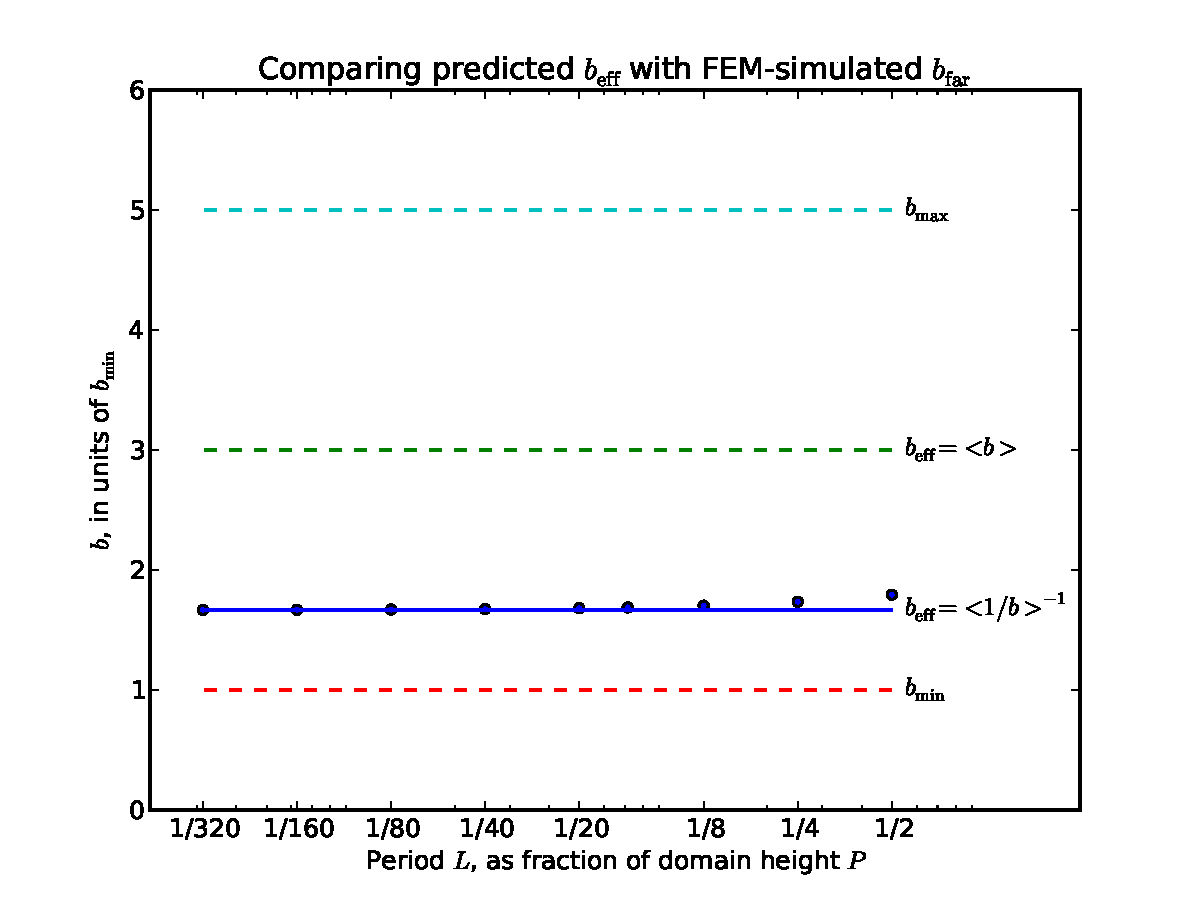
\includegraphics[scale=0.595]{Lund_Thesis_FEM_plot_flat_L}
% Absurd scale factor is to suppress the error message!
\caption{Comparison of numerical $\bfar$ values with predicted $\beff$ for different period sizes, with $b \sim P$.  The dots are values of $\bfar$.  The solid line is the $\beffh$ prediction.}\label{FEMplotflatL}
\end{figure}

As Figure (\ref{FEMplotflatL}) shows, if $b \sim P$, the harmonic mean $\beffh$ formula is an excellent approximation of $\bfar$ if $L \ll P$, and still a good approximation even if $L \sim P$.  Thus, at least in this numerical simulation, the requirement $L \ll P$ is in practice met by the condition $L \leq \frac{1}{10}P$.

\clearpage
\subsubsection{Simple Mean Formula}

The perturbation analysis also yielded a formula $\beffm$ in the limit of vanishing slip length.  This simple area-weighted mean was derived assuming $L \ll P$, and is expected to be a good approximation to $\bfar$ in the limit $b \ll L \ll P$.  To explore this, we ran a series of FEM simulations with fixed $L = \frac{1}{10}P$, and $\bmax$ varying from $\bmax = P$ down to $\bmax = \frac{1}{400}P$.  The $\bfar$ of each simulation is plotted as a dot in Figure (\ref{FEMplotflatb}).
%\clearpage

\begin{figure}[ht]
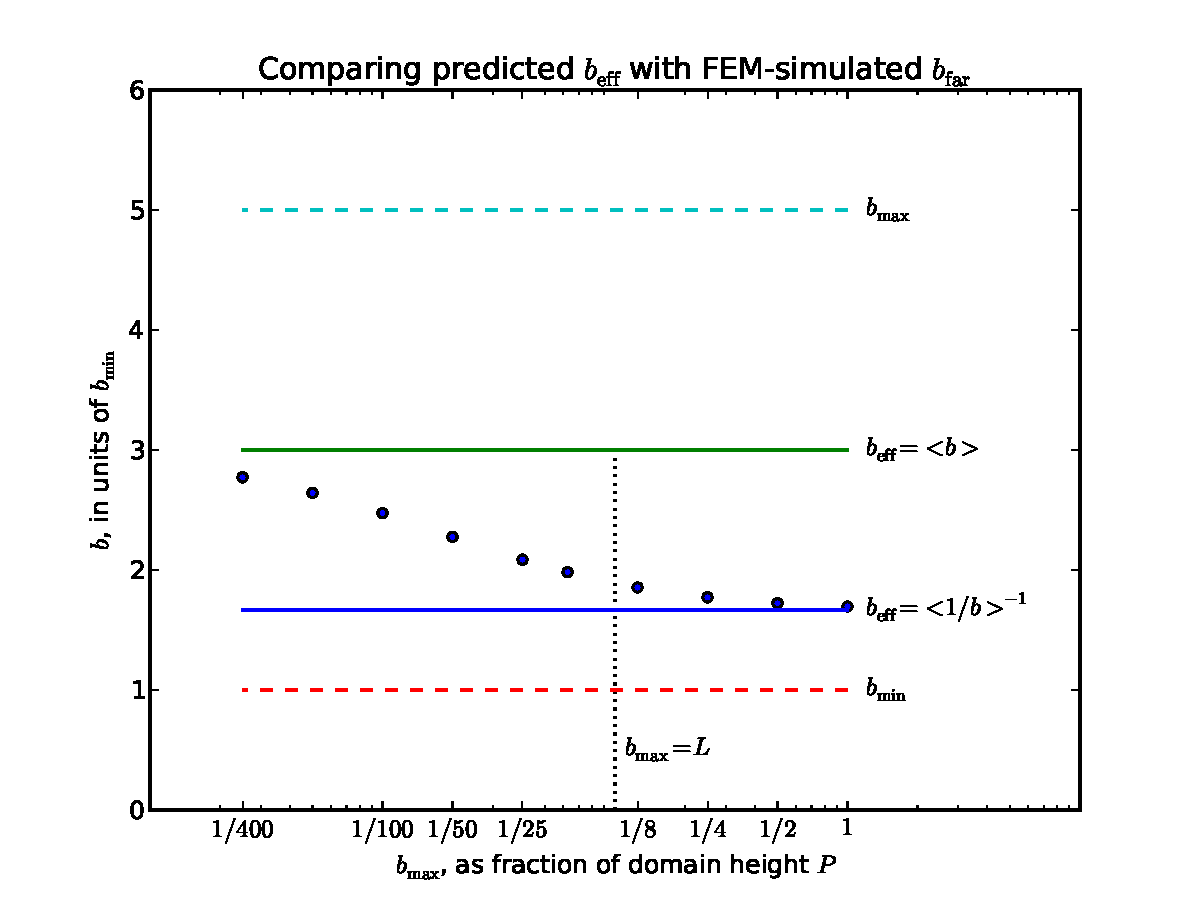
\includegraphics[scale=0.595]{Lund_Thesis_FEM_plot_flat_b}
% Absurd scale factor is to suppress the error message!
\caption{Comparison of numerical $\bfar$ values with $\beff$ predictions, for different values of $\bmax$, with $L = \frac{1}{10}P$. The dots are values of $\bfar$. The lower solid line is the $\beffh$ prediction, and the upper solid line is $\beffm$ prediction.  The vertical dotted line indicates where $\bmax = L$.}\label{FEMplotflatb}
\end{figure}

The values of $\bfar$ in Figure (\ref{FEMplotflatb}) demonstrate a gradual transition from the regime where $\beffh$ applies to the regime where $\beffm$ applies.
Figure (\ref{FEMplotflatb}) affirms that $\beffh$ is an excellent approximation in the regime $L \ll b,P$, and reveals that $\beffh$ is a surprisingly good approximation in the regime $ L \sim b \ll P$.
 The `limit of vanishing slip length' is shown to be quite a strong condition: The regime $b \approx \frac{1}{1	0} L \ll P$ is a `transition regime', with the $\bfar$ values midway between the simple mean and the harmonic mean; the simple mean is not a good approximation until $\bmax \leq \frac{1}{40}L$.

\clearpage
\subsection{Rough Surface}

The FEM testing on a flat surface showed our harmonic mean $\beffh$ formula to be an excellent approximation in the regime $L \ll P, \bmax$.  We now wish to investigate the importance of the arc-length correction -- the correction due to the increased area of liquid-solid contact on a rough surface.

To that end, we ran a series of FEM simulations with sinusoidal surfaces. Each surface was a corrugation with the standard sine-wave profile -- the amplitude and period are always in the ratio $1:2\pi$.  The slip length varied in a binary fashion, with high slip in the valleys of the sinusoid, and low slip on the peaks of the sinusoid.  This models a nanograting with air pockets in the grooves.  The flow was shear-driven by a fixed shear rate, and the slip lengths were fixed at $\bmin = \frac{1}{5} P, \; \bmax = P$.  A schematic appears in Figure (\ref{FEMroughmodel}).

\begin{figure}[ht]
\centering
\begin{tikzpicture}
\node at (3.7,5) {Top Boundary Condition: $\frac{\partial u}{\partial z} = 1 $};

\draw[->, ultra thick] (3,4) -- ++(3,0);
\draw[->, ultra thick] (3,3) -- ++(2,0);
\draw[dashed] (3,2.5) ++(1.5,0) -- ++(2.5,2.5);

% \L = 3.2; length of period
\fill [color=yellow,domain=0:8,samples=200] plot (\x,{ (3.2 /6.2823) * sin( 6.2832 *\x / 3.2 r)} ) -- ++(0,-3) -| (0,0);

\draw[color=white,fill=white] (1.6,0) rectangle ++(1.6,-1.6);
\draw[color=white,fill=white] (4.8,0) rectangle ++(1.6,-1.6);

\draw [domain=0:8,samples=200] plot (\x,{ (3.2 /6.2823) * sin( 6.2832 *\x / 3.2 r)} );

\draw[<->] (3.2,-2.3) -- node[above] {$L$} ++(3.2,0);

\renewcommand{\baselinestretch}{1.00}
\node at (2.4,-1.1) [align=center] {High \\ Slip};
\node at (4,-0.2) [align=center] {Low\\ Slip};


\end{tikzpicture}
\caption{Schematic of the FEM model with corrugated mixed-slip surface.}\label{FEMroughmodel}
\end{figure}

A series of FEM simulations were done with different periods of the sinusoidal corrugation, starting from $L = \frac{1}{2}P$, down to $L = \frac{1}{200}P$. The $\bfar$ from each simulation appears as a dot in the plot of Figure (\ref{FEMplotsine}).

\begin{figure}[ht]
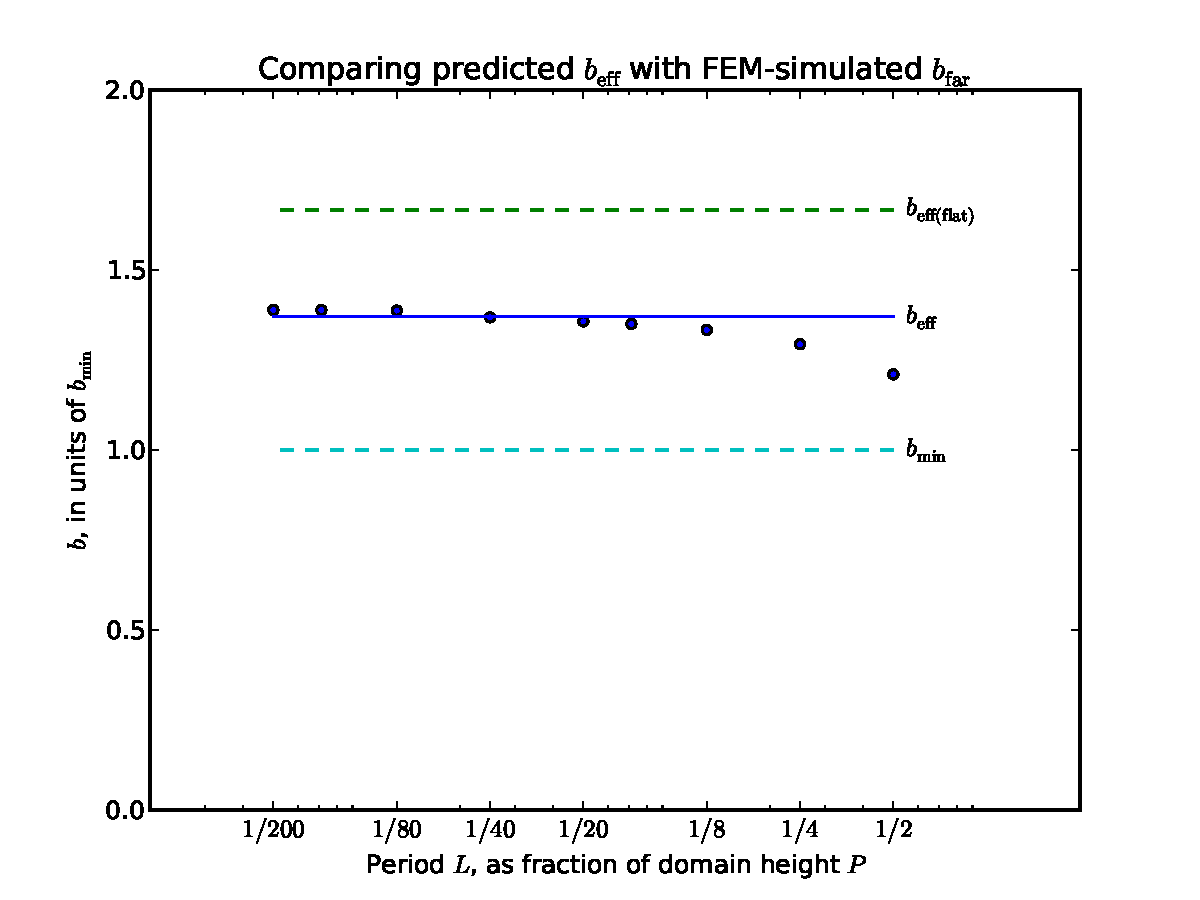
\includegraphics[scale=0.595]{Lund_Thesis_FEM_plot_sine}
% Absurd scale factor is to suppress the error message!
\caption{Comparison of numerical $\bfar$ values with $\beff$ predictions for \textbf{sinusoidal} surfaces for different periods, with $b\sim P$. The dots are values of $\bfar$. The solid line is the  $\beffha$ prediction.  The upper dashed line is the $\beffhf$ predicted if the surface were assumed to be flat.}\label{FEMplotsine}
\end{figure}

Figure (\ref{FEMplotsine}) clearly shows the significance of the arc length correction: The full $\beffha$ expression with arc length correction is shown as the solid line, and the $\bfar$ values converge on this line as $L$ gets smaller. The $\beffhf$ calculated if the surface were assumed to be flat is shown as the upper dotted line.  Thus, if $b\sim P$, then the full $\beff$ prediction is an excellent approximation when $L \ll P$.

To better test the accuracy of the $\beff$ prediction, we calculated the differences between the $\bfar$ values and $\beff$, expressed as a percentage of $\beff$.  The resulting percentage differences are plotted in Figure (\ref{FEMplotsinepcnt}). 

\clearpage
\begin{figure}[ht]
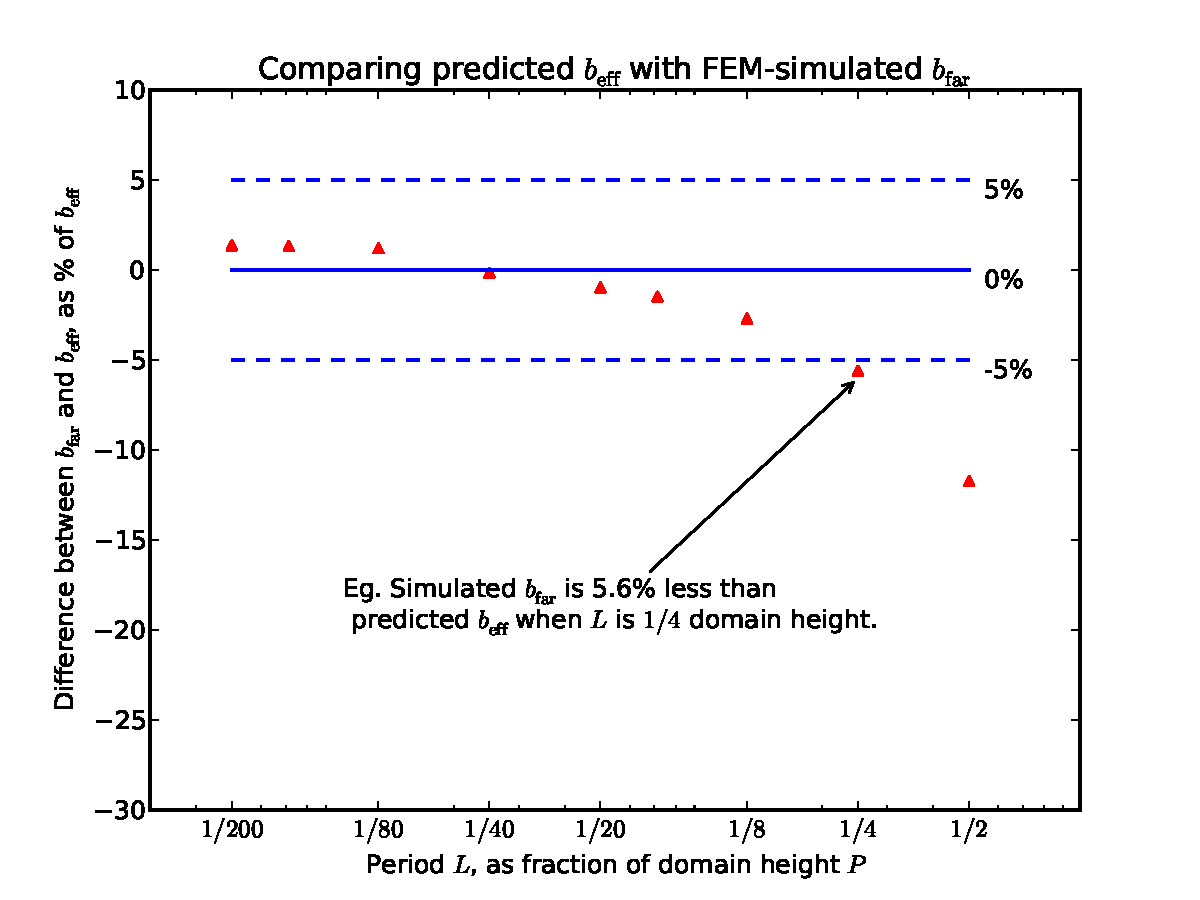
\includegraphics[scale=0.595]{Lund_Thesis_FEM_plot_sine_pcnt}
% Absurd scale factor is to suppress the error message!
\caption{Percentage comparisons between numerical $\bfar$ values and contact-area-corrected $\beffha$ predictions. The dots are values of $\bfar$, expressed as the percentage $(\bfar -\beff)/\beff \times 100 $. }\label{FEMplotsinepcnt}
\end{figure}

The percentage differences of Figure (\ref{FEMplotsinepcnt}) reveal that our contact-area-corrected $\beffha$ prediction for rough surfaces is accurate to within a few \% when $L \ll P, \bmax$.
For example: Accurate to within 5\% when $L \leq \frac{1}{5}P$, and within 1\% when $L$ is less than 5\% of $P$.

The slip lengths in these FEM simulations were calculated with respect to the $z=0$ line, about which the sinusoids oscillate.  In Chapter 3 we noted the ambiguity in the definition of slip length -- does the surface begin at the $z=0$ line or at the tops of the sine wave peaks?  To investigate this issue, we recalculated the measured slip lengths with respect to the \textbf{tops of the peaks}.  These are plotted as the crosses in Figure (\ref{FEMplotsinecorr}) (along with the `uncorrected' slip lengths).

\clearpage
\begin{figure}[ht]
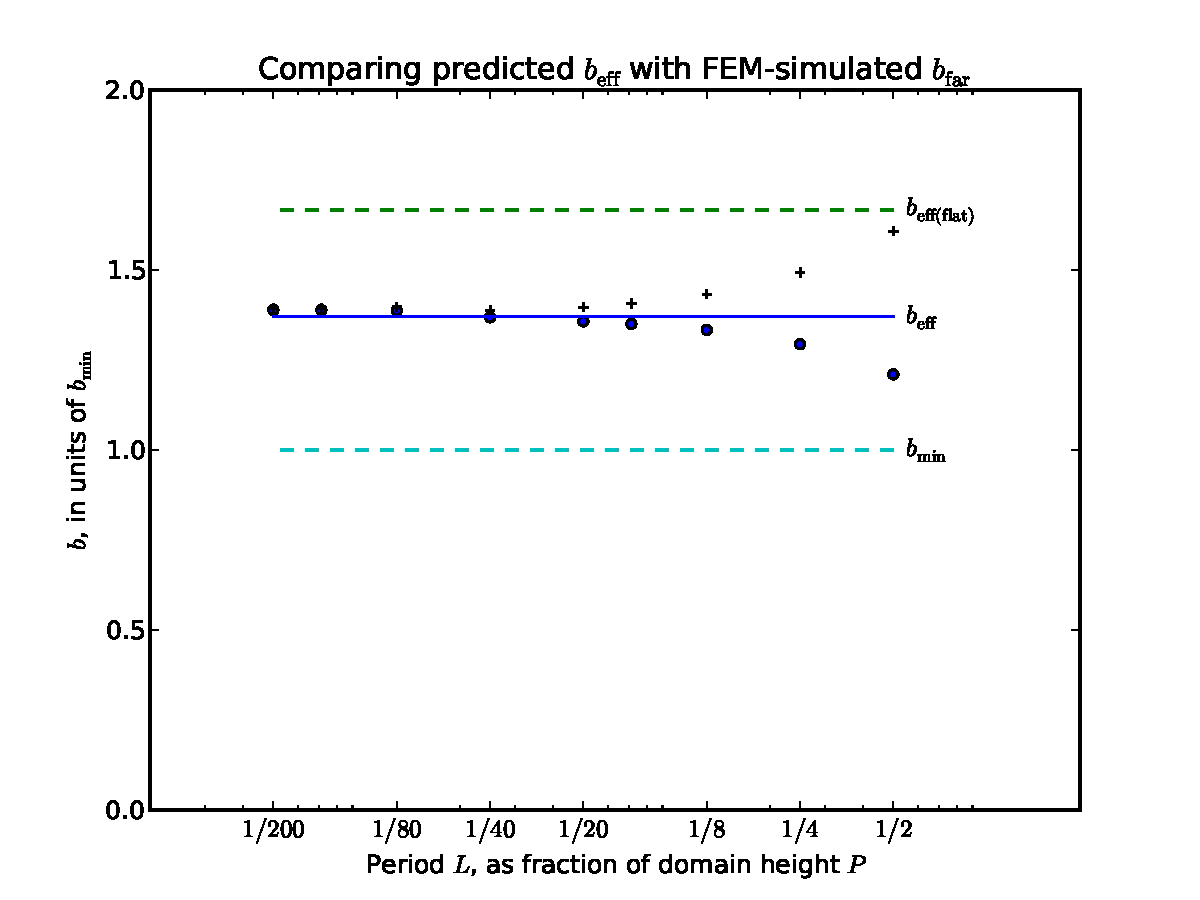
\includegraphics[scale=0.595]{Lund_Thesis_FEM_plot_sine_corr}
% Absurd scale factor is to suppress the error message!
\caption{Comparison of numerical $\bfar$ values with $\beff$ predictions for \textbf{sinusoidal} surfaces for different periods, with $b\sim P$. The dots are values of $\bfar$ calculated w.r.t. the $z=0$ line, and the crosses are $\bfar$ values calculated w.r.t. the top of the sinusoid. The solid line is the $\beffha$ prediction.  The upper dashed line is the $\beffhf$ predicted if the surface were assumed to be flat.}\label{FEMplotsinecorr}
\end{figure}

Figure (\ref{FEMplotsinecorr}) shows that the slip lengths defined with respect to the tops of the surface peaks differ from the predicted $\beff$ by about the same amount as the $z=0$ based slip lengths -- but in the other direction.
In other words, for a given period $L$, the predicted $\beff$ value lies between the two numerical $\bfar$ values calculated with respect to the two different reference points.  The difference between the two types of $\bfar$ values increases as $L$ increases, because the roughness amplitude increases in concert. 
The accuracy of $\beff$ depends on how the measured $\bfar$ values are calculated, and
the `correct' way to calculate $\bfar$ depends on the circumstance.  If effective slip lengths are measured with respect to the tops of the roughness, then our $\beff$ predictions will underestimate measured effective slip lengths. 
%; without being quantitative, Figure (\ref{FEMplotsine3}) suggests that neither of the two types of $\bfar$ considered give rise to significantly better accuracy than the other. 

%\clearpage
A final note about numerical issues:  A close look look at the data plotted in Figure (\ref{FEMplotsinepcnt}) reveals that the numerics and the prediction agree better and better as $L$ gets smaller and smaller --- up to a point.  Then the prediction \emph{underestimates} the numerical values.  We believe this to be a computational artefact, due to an insufficient number of lattice points  on a very rapidly oscillating boundary:  When we noticed that the $\bfar$ values overshot the prediction, we ran the same simulations with double the number of lattice points.  The overshoot reduced, so we further increased the number of lattice points, which gave even better results.  At some point we hit the limit of our computional power, but it is reasonable to think that given sufficient computational power, the discrepancy would disappear.
  
%As the FEM simulations were tuned using finer and finer mesh granularity, the $\bfar$ values overshot $\beff$ by less and less, suggesting that the overshoot is due to an insufficient number of lattice points on a very rapidly oscillating boundary.

%As the simulations were tuned, using finer and finer mesh granularity, in the regime $L \ll P$, the $\bfar$ values got closer and closer to predicted $\beff$ (overshooting by less and less).  Extrapolating to the limit of infinite computing power, we suggest that the numerics would \emph{never} overshoot $\beff$, and the overshoot seen here is due to an insufficient number of lattice points on a very small and rapidly oscillating sine wave boundary.








\clearpage
\section{Finite Difference Numerics}

As an exercise, the same slip problem was also solved numerically using the finite difference method.  The main benefit of this exercise (apart form educational) was that the software employed allowed the easy visualisation of 3-dimensional flow fields.  We employed Python using the Numpy library, which is a front end to various very fast C and Fortran libraries, and the Mayavi library for visualisation.  A curved boundary is difficult to implement in this approach, so the case of the flat slip boundary was studied.

Three-dimensional velocity profiles were generated.  The $x$-velocity $u$ for flow over a mixed-slip surface is shown in Figure (\ref{flow}).

\begin{figure}[ht]
\centering
\begin{tikzpicture}
\node [above right] { 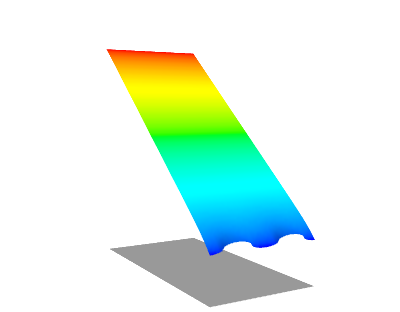
\includegraphics[scale=0.595]{Lund_Thesis_Flow} };

\coordinate (origin) at (4.53,0.22);
\draw[->] (origin) -- node[below]{$x$} ++(11:3cm);
\draw[->] (origin) -- node[below]{$z$} ++(150:2.5cm) -- node[left]{$u$} ++(0,5);
\draw (origin) ++(150:2.5cm) ++(0,4.17) -- ++(-0.15,0) node[left] {$u_P$};

\node at (6.8,1.65)[right]{$u$ with mixed-slip boundary};
\end{tikzpicture}
\caption{The coloured surface is $u$, the $x$-velocity component of a velocity field of a finite difference simulation of flow over a flat mixed-slip surface.}\label{flow}
\end{figure}


The $x$-velocity is high and uniform at the top boundary condition (large $z$), and varies periodically over the slip boundary.

\clearpage
To provide some perspective, flow profiles over \emph{pure} high-slip and low-slip surfaces were generated.  These are plotted together, along with the mixed-slip flow profile, in Figure (\ref{flowhilo}).

\begin{figure}[ht]
\centering
\begin{tikzpicture}
\node [above right] { 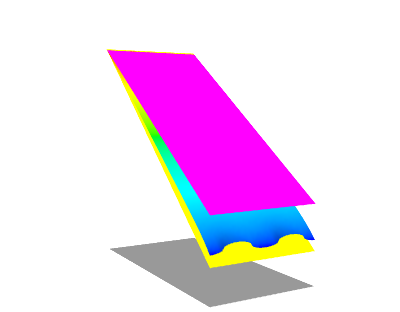
\includegraphics[scale=0.595]{Lund_Thesis_Flow_HiLo} };

\coordinate (origin) at (4.53,0.22);
\draw[->] (origin) -- node[below]{$x$} ++(11:3cm);
\draw[->] (origin) -- node[below]{$z$} ++(150:2.5cm) -- node[left]{$u$} ++(0,5);
\draw (origin) ++(150:2.5cm) ++(0,4.15) -- ++(-0.15,0) node[left] {$u_P$};

\node at (6.6,2.7)[right]{$u$ with high-slip boundary};
\node at (6.6,1.8)[right]{$u$ with mixed-slip boundary};
\node at (6.6,1.25)[right]{$u$ with low-slip boundary};

\end{tikzpicture}
\caption{The same mixed-slip flow field as in Figure (\ref{flow}), plus the flow solutions for flow over the purely high-slip surface (pink), and the purely low-slip surface (yellow).}\label{flowhilo}
\end{figure}

There is an interesting feature in the mixed-slip flow field: while the velocity at the slip boundary varies periodically, the variation is not very large.  The slip velocity does \emph{not} swing between the extremes of velocities over the pure high-slip and low-slip surfaces.  Instead, the slip velocity has only a moderate periodic variation about a central value.

What is that central value?  Of course, we expect it to be the slip velocity that would occur if the surface had a single slip length equal to our predicted $\beff$.
We explore this by generating a last flow profile with a pure $\beff$ slip length surface.  We plot this (in black) together with the mixed-slip flow profile in Figure (\ref{floweff}).

\clearpage
\begin{figure}[ht]
\centering
\begin{tikzpicture}
\node [above right] { 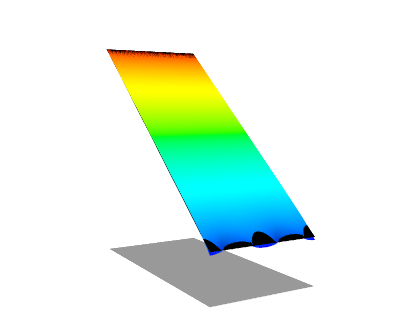
\includegraphics[scale=0.595]{Lund_Thesis_Flow_Eff} };

\coordinate (origin) at (4.53,0.22);
\draw[->] (origin) -- node[below]{$x$} ++(11:3cm);
\draw[->] (origin) -- node[below]{$z$} ++(150:2.5cm) -- node[left]{$u$} ++(0,5);
\draw (origin) ++(150:2.5cm) ++(0,4.17) -- ++(-0.15,0) node[left] {$u_P$};

\node at (6.7,1.9)[right]{$u$ with $\beff$ slip boundary (black)};
\node at (6.6,1.45)[right]{$u$ with mixed-slip boundary};
\end{tikzpicture}
\caption{The same mixed-slip flow field as in Figure (\ref{flow}), plus the flow field corresponding to a homogeneous boundary of slip length $\beff$ (black).}\label{floweff}
\end{figure}

Figure (\ref{floweff}) shows excellent agreement between the effective flow profile and the mixed-slip profile.  For most of the domain, they are almost indistinguishable.  Only very close to the slip boundary does the mixed-slip profile exhibit a periodic variation about the effective slip profile.

\vspace{1em}

The plot of Figure (\ref{floweff}) also throws light on another issue: how thick is the boundary layer?  The boundary layer can be  arbitrarily defined to end where the flow becomes (arbitrarily close to) uniform.  Without being quantitative, we can see that a reasonable choice for boundary layer thickness $d$ could be less than the period $L$.
%  This would explain why the FEM simulations showed that $\beff$ works unexpectedly well even when it is not strictly true that $L \ll \bmin$.  The explanation is that even when $L \sim \bmin$, it may still be true that $d < \bmin$.  

%Finally, recall that the condition $L \ll \bmin$ is not a `requirement' as such.  In the mathematical model, $L$ and $\bmin$ are the appropriate nonarbitrary length scales, and the expression for $\beff$ becomes more and more exact as $L \to 0$.  To summarise the concept `$L$ is closer to zero than $\bmin$ is close to zero', one simply states that $L \ll \bmin$.


\clearpage
\section{Conclusion}

Numerical simulations reveal that if the period of surface patterning $L$ is much less than the domain height $P$ and typical slip lengths, then the effective slip length as defined in the far field of the system is very well approximated by:
\begin{equation}
\beff = \left<  \frac{\sqrt{1 + |\nabla h  |^2}}{b} \right> ^{-1}
\label{eq:harm}
\end{equation}
The $\beff$ expression incorporates a correction for the increased area of solid-liquid contact in rough surfaces.  Numerical testing shows this correction to be accurate, so therefore our $\beff$ expression of Equation (\ref{eq:harm}) is valid for both flat and rough surfaces.

Numerical simulations further reveal that if $L \ll P$ and slip lengths are of the same order as the period, $L \sim b$, then Equation (\ref{eq:harm}) is a surprisingly good approximation for effective slip lengths.

If slip lengths are much smaller than any other length scale, then the effective slip length is best approximated by a simple area-weighted mean.  Numerical testing with a flat surface showed that if $\bmax \leq \frac{1}{40} \ll P$, then the effective slip length is well approximated by:
\begin{equation}
\beff = \langle b \rangle
\end{equation}




\iftoggle{compilealone}
    {
    \bibliography{Lund_Thesis.bib}
    \bibliographystyle{plain}
    }

\end{document}




\clearpage
\subsection{Rough Surface (Old)}

Using FreeFem++, we modelled a two-dimensional fluid.  The fluid was driven by a fixed shear rate at the top boundary.  The slip boundary at the bottom was a sine wave profile, with an intrinsic slip length that varied in a binary fashion with the same period: The slip length on the peak of the sine wave was a low value, and the slip length on the trough of the sine wave was a high value.  This models shear-driven flow transverse to a grating or corrugation, with an air pocket in the grooves. 
A schematic is shown in Figure (\ref{FEMmodel}).


\begin{figure}[ht]
\centering
\begin{tikzpicture}
\node at (3.7,5) {Top Boundary Condition: $\frac{\partial u}{\partial z} = 1 $};

\draw[->, ultra thick] (3,4) -- ++(3,0);
\draw[->, ultra thick] (3,3) -- ++(2,0);
\draw[dashed] (3,2.5) ++(1.5,0) -- ++(2.5,2.5);

% \L = 3.2; length of period
\fill [color=yellow,domain=0:8,samples=200] plot (\x,{ (3.2 /6.2823) * sin( 6.2832 *\x / 3.2 r)} ) -- ++(0,-3) -| (0,0);

\draw[color=white,fill=white] (1.6,0) rectangle ++(1.6,-1.6);
\draw[color=white,fill=white] (4.8,0) rectangle ++(1.6,-1.6);

\draw [domain=0:8,samples=200] plot (\x,{ (3.2 /6.2823) * sin( 6.2832 *\x / 3.2 r)} );

\draw[<->] (3.2,-2.3) -- node[above] {$L$} ++(3.2,0);

\renewcommand{\baselinestretch}{1.00}
\node at (2.4,-1.1) [align=center] {High \\ Slip};
\node at (4,-0.2) [align=center] {Low\\ Slip};


\end{tikzpicture}
\caption{Schematic of the model used in the finite element analysis.}\label{FEMmodel}
\end{figure}

\clearpage
Specifics:  The minimum slip length was $\bmin = 1$, the maximum slip length was $\bmax = 5$, the   height of domain was $P = 20$, and the fixed shear rate at $P$ was 1 s$^{-1}$.  The sinusoidal surface was centered at $z=0$, with $\bmin$ on the peaks and $\bmax$ in the troughs.   With $\bmax$ at 25\% of domain height $P$, this regime is \emph{not} near the limit of vanishing slip length, so we expect the homogenized area-weighted harmonic mean formula to apply.  The formula predicts $\beff = 1.36$.

The FEM analysis was done for a series of sinusoidal slip surfaces, each with a different period $L$, but with the same values of $\bmin$ and $\bmax$.  For each $L$, an effective slip length $\bfar$ was calculated from the far-field velocity field solution. These are plotted as the dots in Figure (\ref{FEMplot}).  
The predicted $\beff$ appears as a solid line.  
Period $L$ is expressed as a fraction of $P$.

%The FEM solution for each surface is a velocity field; from the far-field part of this solution an effective slip length $\bfar$ was calculated. 
% The fixed slip lengths and the sine wave profile were plugged into our formula, generating $\beff$.  The results are plotted in Figure (\ref{FEMplot}).  The solid line is the predicted $\beff$ (which does not depend on $L$), and the dots are the simulated $\bfar$ values at various values of $L$.


\begin{figure}[ht]
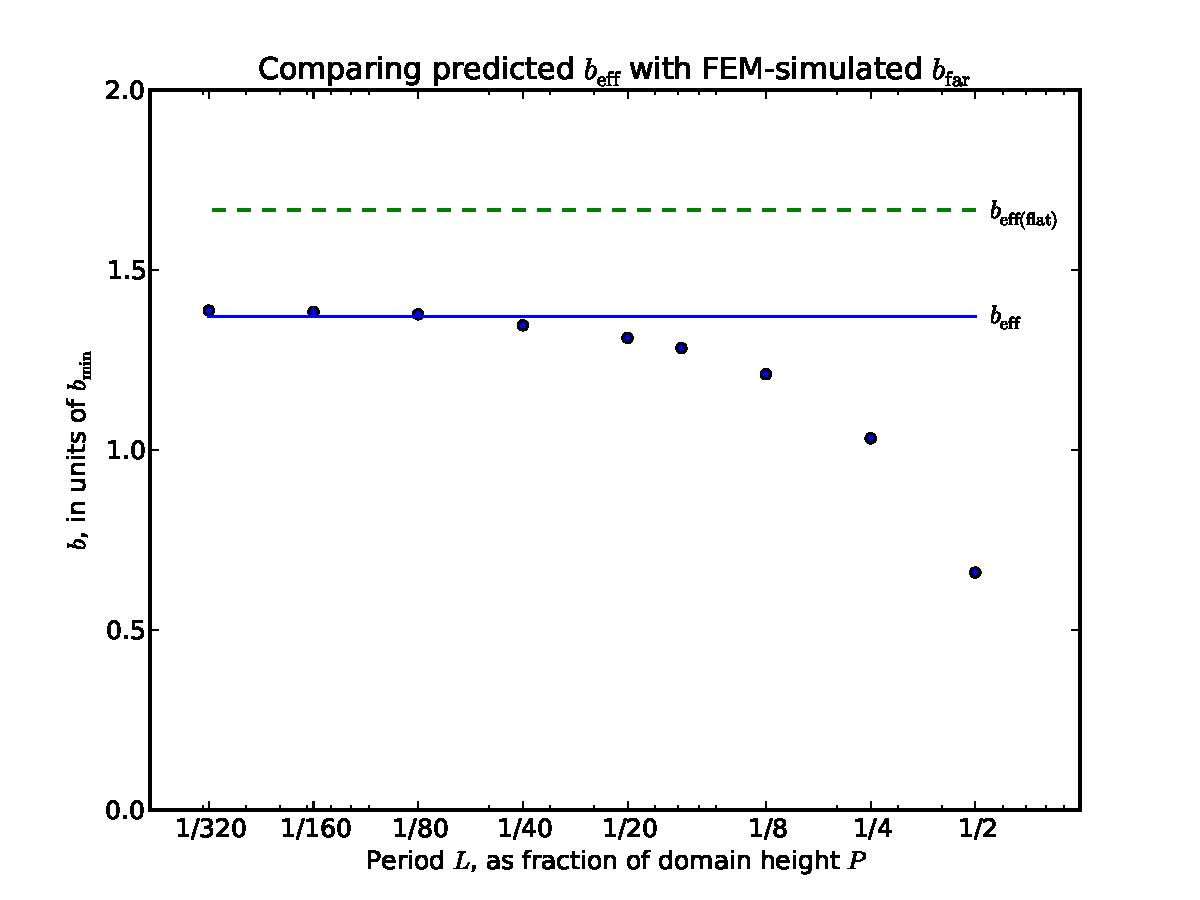
\includegraphics[scale=0.595]{Lund_Thesis_FEM_plot_LonP}
% Absurd scale factor is to suppress the error message!
\caption{Dots are values of $\bfar$ -- the effective slip length values calculated from the far-field velocity solutions of FEM simulations.  Solid line is the predicted $\beff$.  Dotted line is the $\beff$ predicted if the surface were assumed to be flat. }\label{FEMplot}
\end{figure}

As noted, a system is `near the limit' if $L \ll P$, in which case the predicted $\beff$ should approximate measured $\bfar$ very well.  Figure (\ref{FEMplot}) shows this to be true.

%As noted, a system is `near to the limit' if $L \ll \bmin$, in which case the predicted $\beff$ should approximate measured $\bfar$ very well.  This is true.  At $L = 0.1 \bmin$, the plot shows the numerically-calculated $\bfar$ (dots) to be within a few percent of predicted $\beff$ (solid line).

For interest,
the dashed green line is the effective slip length calculated if the surface were naively assumed to be flat.  Comparison with the numerical values shows the importance of the correction from using true contact area: the naive flat calculation overshoots numerical slip lengths by about 20\%.



%But the pleasant surprise is that our full roughness-corrected $\beff$ prediction appears to be good even where $L \sim \bmin$.
%For ease of comparing relative magnitudes, in Figure (\ref{FEMplotpcnt}) we plot the data with $\bfar$ expressed as a percentage difference from $\beff$.


To better quantify the success of our $\beff$ prediction, we plot the same data with $\bfar$ expressed as a percentage difference from $\beff$.  This is shown in Figure (\ref{FEMplotpcnt}).

\begin{figure}[ht]
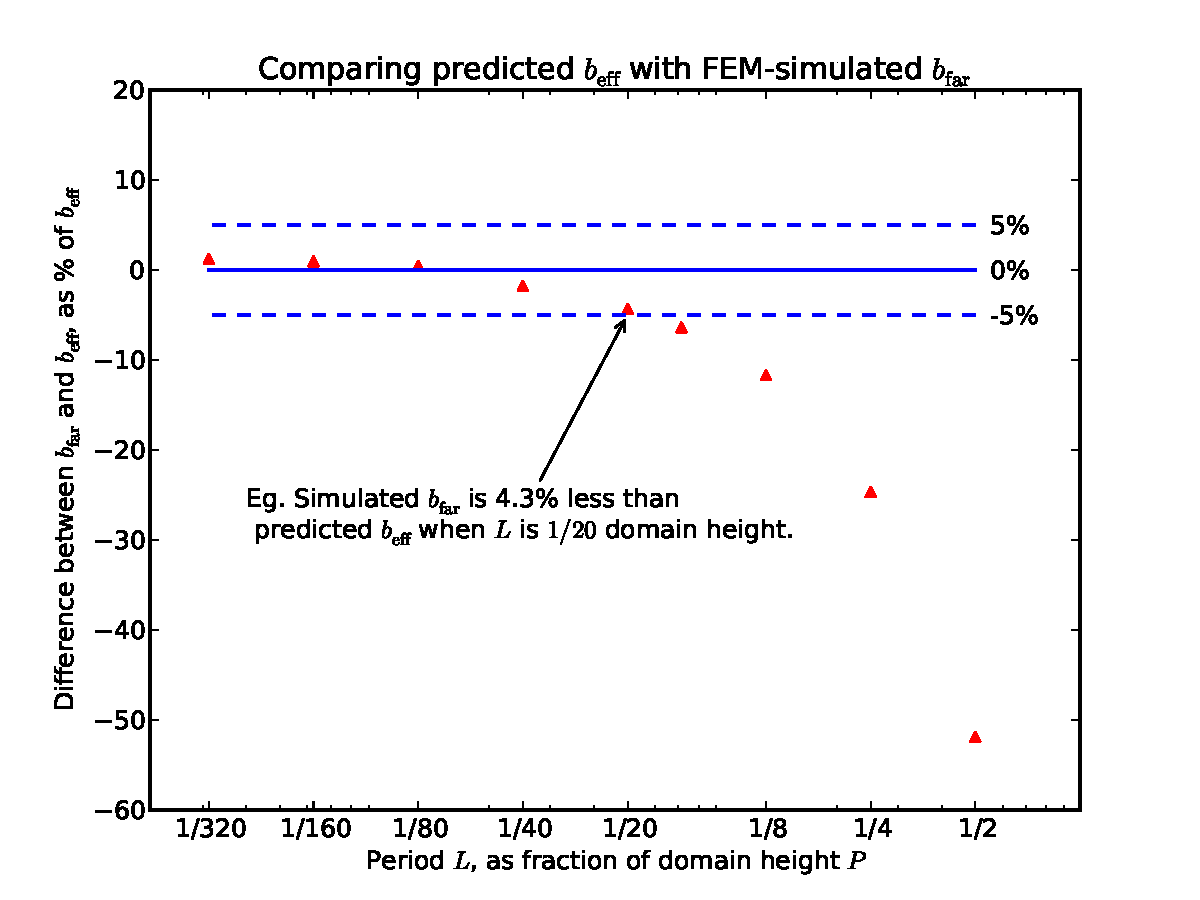
\includegraphics[scale=0.595]{Lund_Thesis_FEM_plot_pcnt_LonP}
% Absurd scale factor is to suppress the error message!
\caption{Triangles are values of $\bfar$ -- effective slip lengths from FEM simulations.  Solid line is predicted $\beff$.  Dashed lines are 5\% above and below $\beff$.}\label{FEMplotpcnt}
\end{figure}

We see that if $L$ is 5\% of $P$, then the numerical results differ from our prediction by less than 5\%.
In fact the data suggest a rough rule of thumb: if $L$ is $x$\% of $P$, measured $\bfar$ will be $x$\% less than predicted $\beff$.



%So, while \emph{a priori} we can only expect our prediction to be trustworthy if $L \ll \bmin$, in practice --- or at least in this numerical simulation --- our prediction is very good for much larger values of roughness period, where $L \leq \bmin$.

%\clearpage
The slip lengths in these FEM simulations were calculated with respect to the $z=0$ line, about which the sinusoids oscillate.  In Chapter \ref{C:mixedslip} we noted the ambiguity in the definition of slip length -- does the surface begin at the $z=0$ line or at the tops of the sine wave peaks?  To investigate this issue, we recalculated the measured slip lengths with respect to the \textbf{tops of the peaks}.  These are plotted as the crosses in Figure (\ref{FEMplotcorrected}) (along with the `uncorrected' slip lengths).

\begin{figure}[ht]
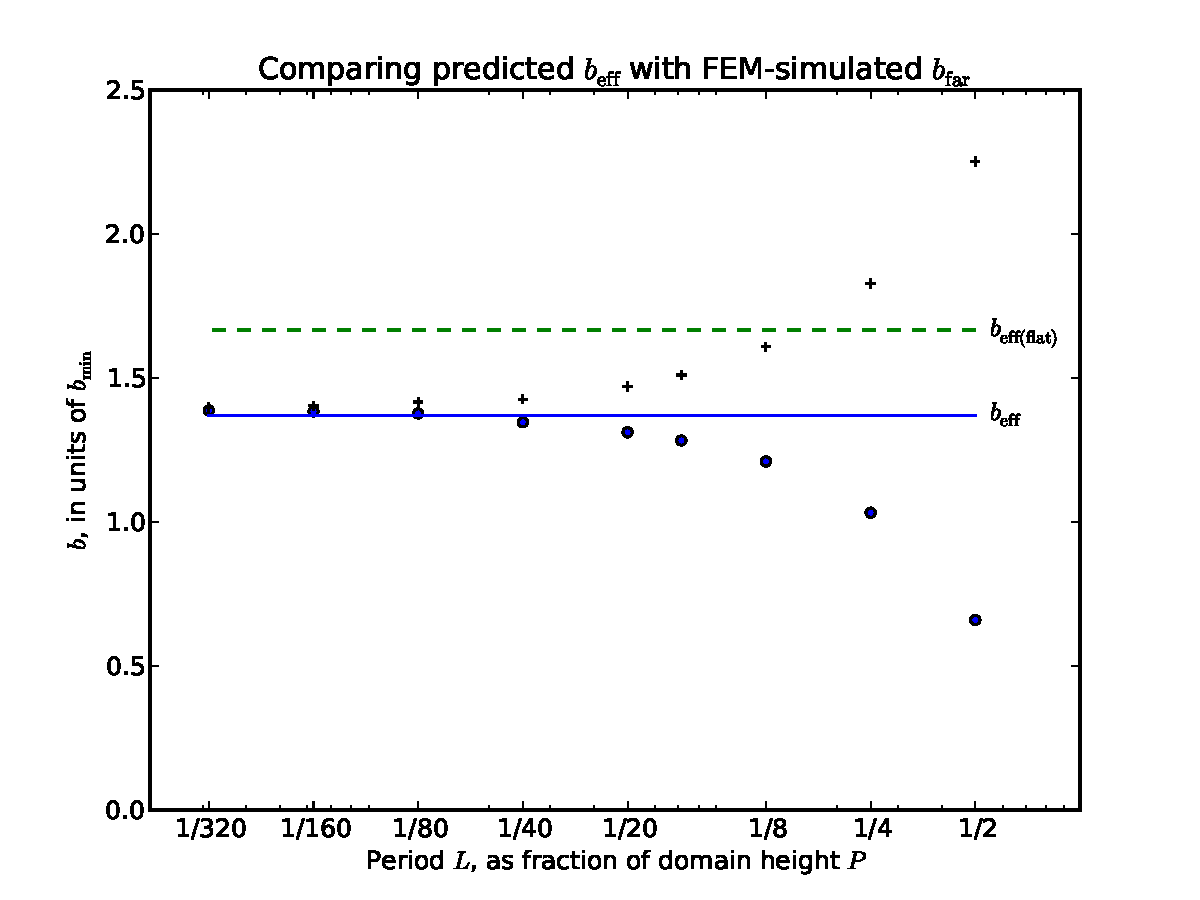
\includegraphics[scale=0.595]{Lund_Thesis_FEM_plot_LonP_corrected}
% Absurd scale factor is to suppress the error message!
\caption{Dots are values of $\bfar$, as in Figure (\ref{FEMplot}).  Crosses are $\bfar$ calculated w.r.t the tops of the surface peaks.  Solid line is the predicted $\beff$.  Dotted line is the $\beff$ predicted if the surface were assumed to be flat. }\label{FEMplotcorrected}
\end{figure}

Figure (\ref{FEMplotcorrected}) shows that the slip lengths defined with respect to the tops of the surface peaks differ from the predicted $\beff$ by about the same amount as the $z=0$ based slip lengths -- but in the other direction.  The good news is that our predicted $\beff$ is pretty much in the middle of the defensible range of measured slip lengths.


Note that while the homogenized $\beff$ is expected to work when $L \ll P$, the perturbation method \emph{assumed} $L \ll P$, and the result was considered valid when $b \sim P$.  The example here, with $\bmin$ = 10\% of $P$, and $\bmax$ = 25\% of $P$, is on the borderline of this requirement.  But the result still works excellently.  This suggests that the requirement of the perturbative result is not fundamental, and affirms that homogenization is a stronger technique. 

A final note about numerical issues:  A close look look at the data plotted in Figures (\ref{FEMplot}) and (\ref{FEMplotpcnt}) reveals that the numerics and the prediction agree better and better as $L$ gets smaller and smaller --- up to a point.  Then the prediction \emph{underestimates} the numerical values.  We believe this to be a computational artefact.  As the simulations were tuned, using finer and finer mesh granularity, in the regime $L \ll P$, the $\bfar$ values got closer and closer to predicted $\beff$ (overshooting by less and less).  Extrapolating to the limit of infinite computing power, we suggest that the numerics would \emph{never} overshoot $\beff$, and the overshoot seen here is due to an insufficient number of lattice points on a very small and rapidly oscillating sine wave boundary.

% Finished September 26, 2013
% Put into VUW Thesis format Wednesday 2 April 2014

\documentclass[12pt, a4paper, twoside, openright]{book}

\usepackage{vuwthesis} % sets up some local things, mostly the front page

\setlength{\intextsep}{12pt} % set space above and below in-line float
\setlength{\abovecaptionskip}{0pt} % set space between figure and caption.


\usepackage{amssymb, amsmath}
%\usepackage{mathtools}
\usepackage{tikz}
\usetikzlibrary{calc}
\usepackage{url}

%\usepackage{marvosym}

\newcommand{\beff}{\ensuremath{b_{\mathrm{eff}}}}
\newcommand{\bmin}{\ensuremath{b_{\mathrm{min}}}}
\newcommand{\bmax}{\ensuremath{b_{\mathrm{max}}}}
\newcommand{\bfar}{\ensuremath{b_{\mathrm{far}}}}

\newcommand{\Tr}{\ensuremath{T_{\mathrm{room}}}}

\newcommand{\Finc}{\ensuremath{F_{\mathrm{inc}}}}
\newcommand{\Fads}{\ensuremath{F_{\mathrm{ads}}}}
\newcommand{\Fdes}{\ensuremath{F_{\mathrm{des}}}}
\newcommand{\Fcat}{\ensuremath{F_{\mathrm{cat}}}}

\newcommand{\kcat}{\ensuremath{k_{\mathrm{cat}}}}

\title{Chapter 9: Analogues of Effective Slip}
\author{Nat Lund}


\begin{document}
\chapter{Analogues of Effective Slip}

We have found the effective slip length for Stokes flow over a periodic mixed-slip surface.  However, on a purely mathematical level we have shown that Laplace's equation with a particular boundary condition:
\begin{gather}
\nabla^2 u = f \\
u = b(x,y) \frac{\partial u}{\partial z}
\end{gather}
has solutions:
\begin{equation}
\beff = \left< \frac{1}{b} \right>^{-1} \text{   if   } L \ll \bmin, \qquad \text{and} \qquad
\beff = \left< b \right> \text{   if   } \bmin \ll L
\end{equation}
Where $b$ is some periodic function on the boundary with units of length and period $L$.

\vspace{1em}
This models our slip problem.  The obvious question is: what other physical systems does it model?  If we can find appropriate systems, then we automatically have a solution --- some analogue of effective slip length.

We shall investigate two such physical systems forthwith: a thermal insulation problem and a heterogeneous catalyst problem.


\section*{Thermal Insulation}

Consider an atypical New Zealand house: one with insulation in the roof.  A standard house has an angled roof situated above a flat ceiling, with a fairly large crawlspace in between.  The ceiling panels are attached to the underside of wooden beams known as rafters, which are spaced 600 mm apart.  It is traditional to devote several entire weekends to laying insulating material on top of the ceiling panels, in the gaps between the rafters.
Thus, above the warm living space of a house, is a heterogeneous insulator, comprising wood (the rafters), highly insulating material, and those air gaps that are left over because you couldn't be bothered cutting scatchy, unwieldy fibreglass batts to exactly the right size.

\begin{figure}[ht]
\centering
\begin{tikzpicture}
%Walls and ceiling
\draw[fill=brown] (0,0) rectangle ++(-0.5,-3);
\draw[fill=brown] (6,0) rectangle ++(0.5,-3);
\draw[fill=gray] (0,0) rectangle ++(6,-0.1);
\draw[fill=gray] (-1.5,0) rectangle ++(1,-0.1);
\draw[fill=gray] (6.5,0) rectangle ++(1,-0.1);

%Roof
\draw[fill=brown] (-1.5,0) rectangle ++(0.25,0.5);
\draw[fill=brown] (7.5,0) rectangle ++(-0.25,0.5);
\draw[ultra thick] (-1.6,0.5) -- ++(4.6,2) -- ++(4.6,-2);

% Rafters
\foreach \x in {1,2,3}
        {\draw[fill=brown] (-1.5,0) ++(\x*1.9375,0) ++(\x*0.25,0) rectangle ++(0.25,0.5);}

% Fibreglass batts
\foreach \x in {0,1,2,3}
        {\draw[fill=pink] (-1.25,0) ++(\x*1.9375,0) ++(\x*0.25,0) rectangle ++(1.9375,0.5);}

\node at (3,-1.5) {Warm Room};
\node at (2,1) {Rafters};
\draw[<-] (-1.25,0) ++(1.9375,0) ++(0.2,0.625) -- ++(35:0.5cm);
\draw[<-] (-1.25,0) ++(1.9375,0) ++(0.25,0) ++(1.9375,0) ++(0.05,0.625) -- ++(135:0.4cm);
\node at (4.1,0.25) {Insulation};

\end{tikzpicture}
\caption{a}\label{a}
\end{figure}

\subsection*{Mathematical Model}

We are interested in the `net' insulating properties of the heterogeneous insulator comprising wood, insulating material and possibly air gaps.  To that end, we model the heterogeneous insulator as a bulk material
with: a warm room at the lower boundary, and convection-dominated heat loss on the top boundary.  For consistency with our slip model, we shall invert the vertical dimension, and let $z=0$ denote the top of the bulk and $z=d$ the bottom of the bulk.  The temperature field is $T(x,y,z)$, with boundary conditions at $T(x,y,0)$ and $T(x,y,d)$, denoted $T(0)$ and $T(d)$.

\subsubsection*{Dirichlet Condition}

The warm room can be considered to be held at a constant temperature, due to the interventions of its human occupants.  Therefore, on the $z=d$ boundary is the Dirichlet condition
\begin{equation}
T(z) = \Tr = \text{constant}
\end{equation}

\subsubsection*{Bulk Condition}

The distribution of temperature $T$ in a material is governed by the diffusion equation:
\begin{equation}
\frac{\partial T}{\partial t} = \frac{k}{\rho C_p} \nabla^2 T
\end{equation}
where $k$ is the thermal conductivity, and $C_p$ is the specific heat capacity.

We shall assume that the system is at equilibrium, so that the time dependent term vanishes.  Hence, the solid material -- wooden rafters and insulating material -- is governed simply by Laplace's equation:
\begin{equation}
\nabla^2 T = 0
\end{equation}

\subsubsection*{Conductive Heat Current}
Consider a bar of test material of cross-sectional area $A$ clamped between a hot reservoir and a cold reservoir.
The heat current in the bar (Joules per second) depends on the temperature gradient, the thermal conductivity $k$ and the area $A$:
\begin{equation}
\frac{dQ}{dt} = k A \frac{\partial T}{\partial x}
\end{equation}

\begin{figure}[ht]
\centering
\begin{tikzpicture}
\draw[fill=red](0,-0.5) rectangle node{Hot} ++(-2,2);

\draw(0,0) rectangle ++(4,1);
\draw(0,0) ++(4,-0.5)[fill=blue] rectangle node{Cold} ++(2,2);

\draw (2,0.5)[fill=gray] ellipse (0.1cm and 0.5cm);
\node at (2,0) [below] {$A$};

\end{tikzpicture}
\caption{b}\label{b}
\end{figure}

\subsubsection*{Convective Heat Current}
Convection is harder to quantify than conduction.   
A plate at temperature $T$ convecting into an infinite reservoir of gas at temperature $T_0$ shows a heat flux approximately proportional to $(T - T_0)^{5/4}$.
However, consider the experimental setup in the diagram: a body of convecting air between a hot body and a cold body.  For such a system, the heat flux is usually considered to have a simple linear relationship to temperature difference. 

\begin{figure}[ht]
\centering
\begin{tikzpicture}
%\everymath{\displaystyle}

\node at (0,0) {Convecting Air};
\draw[fill=red] (-1.5,-1.5) rectangle node {Hot} ++(3,-1);
\draw[fill=blue] (-1.5,1.5) rectangle node {Cold} ++(3,1);

\node at (3,0)[right] {$\displaystyle \frac{dQ}{dt} = h A (T - T_0) $};

\node at (1.75,-2) {$T$};
\node at (1.75,2)  {$T_0$};

%Curved Arrows
\draw[->,thick] (0.25,0.4) to [out=90,in=180] ++(0.4,0.75) to [out=0,in=90] ++(0.4,-0.75);
\draw[->,thick] (-0.25,0.4) to [out=90,in=0] ++(-0.4,0.75) to [out=180,in=90] ++(-0.4,-0.75);
\draw[<-,thick] (0.25,-0.4) to [out=-90,in=180] ++(0.4,-0.75) to [out=0,in=-90] ++(0.4,0.75);
\draw[<-,thick] (-0.25,-0.4) to [out=-90,in=0] ++(-0.4,-0.75) to [out=180,in=-90] ++(-0.4,0.75);

\end{tikzpicture}
\caption{c}\label{c}
\end{figure}

This is known as Newton's law of cooling, and $h$ is the \emph{heat transfer coefficient.}

\subsubsection*{Convective Boundary Condition}

The highly-conductive steel roof of a house can be presumed to be at the same low temperature $T_0$ as the outside air. Then convection occurs between the bulk heterogeneous insulator and the cold roof, with heat flux \emph{leaving} the boundary given approximately by Newton's law of cooling.

Furthermore, heat flux will arrive \emph{at} the boundary in accordance with the heat conduction equation.

\begin{figure}[ht]
\centering
\begin{tikzpicture}
\draw[fill = brown] (1.5,0) rectangle ++(-4,-2);
\draw (0,0) -- ++(1,-0.667) -- ++(-0.5,0) -- ++(0,-1);
\draw (0,0) -- ++(-1,-0.667) -- ++(0.5,0) -- ++(0,-1);
\draw (0,2) -- ++(1,-0.667) -- ++(-0.5,0) -- ++(0,-1);
\draw (0,2) -- ++(-1,-0.667) -- ++(0.5,0) -- ++(0,-1);

\node at (2,-1)[right] {Flux to boundary: $\displaystyle \frac{dQ}{dt} = k A \frac{\partial T}{\partial z} $};
\node at (2,1) [right] {Flux from boundary: $\displaystyle \frac{dQ}{dt} = h A (T - T_0)$};

\end{tikzpicture}
\caption{d}\label{d}
\end{figure}

Since the boundary is a virtual plane with no heat capacity, the fluxes are always equal:
\begin{equation}
h A (T - T_0) = k A \frac{\partial T}{\partial z}
\end{equation}

For convenience, define the low temperature to be $T_0 = 0$.  Then the convective boundary condition is:
\begin{equation}
T = \frac{k}{h} \frac{\partial T}{\partial z}
\end{equation}

Now the heat transfer coefficient $h$ is constant for the system.  But the thermal conductivity $k$ varies spatiallly because the bulk material is heterogenous.  Therefore define the variable:
\begin{equation}
b(x,y) = \frac{k}{h}
\end{equation}

And we now have a system of equations equivalent to those describing steady shear-driven Stokes flow with Navier slip:
\begin{gather}
\nabla^2 T = 0 \\
T = b \frac{\partial T}{\partial z}
\end{gather}

The function $b(x,y)$ has units of length, and we can now solve to find an effective `insulation length' for the heterogeneous insulation.  To minimize heat loss for a given room temperature, we want the lowest temperature on the convective boundary, which in turn demands the lowest effective insulation length.

\begin{figure}[ht]
\centering
\begin{tikzpicture}
\draw [<->] (0,4) -- (0,0) -- (9,0);
\draw (4,0) -- ++(0,4);
\draw[thick, color=red] (0,3) -- (4,1.5);
\draw[thick, color=red,dashed] (4,1.5) -- (8,0);

\node at (4,0)[below] {0};
\node at (0,0)[below] {$d$};

\draw (0,3) -- ++(-0.1,0);
\node at (-0.1,3)[left] {\Tr};

\draw[<->] (4,-0.7) -- node[below]{\beff} ++(4,0);

\end{tikzpicture}
\caption{e}\label{e}
\end{figure}


\subsubsection*{Ready-Made Solution}

To apply one of the two solutions we have already found, we need to know which regime the system is in.

The heterogeneity of the bulk material is due to the wooden rafters, spaced about half a meter apart.  Thus the period $L \simeq 1$m.
The heat transfer coefficient for air is experimentally determined to be in the range 10 - 100 Wm$^{-2}$K${-1}$.

The thermal conductivity for wood depends on the moisture content: from 0.04 - 0-.12 Wm$^{-1}$K$^{-1}$ for oven-dry wood, and up to 0.4 Wm$^{-1}$K$^{-1}$ for wood with more than 12\% water content.
Typical highly-insulating materials might be polystyrene foam or polyurethane foam, with $k$ = 0.03 Wm$^{-1}$K$^{-1}$, or mineral wool, sheep's wool, or fibreglass wool, at $k$ = 0.04 Wm$^{-1}$K$^{-1}$.
Air itself -- if sufficiently constrained to avoid convection -- has a very low thermal conductivity of $k$ = 0.024 Wm$^{-1}$K$^{-1}$.

Thus values of $b = k/h$ are in the range 0.0003 to 0.012 meters.  Clearly, $b \ll L$ so we are in the regime where the effective insulation length is given by the area-weighted average:
\begin{equation}
\beff = \left< b \right>
\end{equation}


\vspace{1em}
Note that while the boundary condition is heterogeneous -- $b(x,y)$ is a function of position on the boundary plane -- this is due to the fact that \emph{bulk} is heterogeneous.  The coupling occurs because the heat fluxes match at the boundary.

\vspace{1em}
An interesting historical note: The first expression for effective slip is the one by J.R. Philip from 1972.  His method `generalizes a device of Karush and Young'.  The 1952 paper by Karush and Young
dealt with the effect of a periodic array of perfectly insulating stripes or circles, that partially block the loss of heat from a lump of radioactive material.


\section*{Catalysis}

One particularly widespread application of catalysts is in the catalytic converters fitted to the exhaust systems of motorcars.  Efforts are underway to improve these catalysts by the use of nanostructured material.  The improvement is partly from the increased surface area, and partly from a geometric effect: the sharp corners of a catalyst nanoparticle seem to be more active than flat surfaces of the same catalyst.

Thus, it is possible that a nanostructured catalyst has a catalytic activity that varies across a nominal surface  -- the catalyst is heterogeneous, and may be a candidate for modelling as a homogenization problem.  We shall attempt this here.

\vspace*{1em}
Below is a schematic diagram of a catalyst in action.  We shall consider the simplest case of a single gas species -- say N$_2$O$_4$, that diffuses to the surface of the catalyst, where a catalysed reaction breaks the molecule down into separate N$_2$ and O$_2$ molecules.  The catalyst surface has some `sharp bits' that have greater catalytic activity than the flat regions.



\begin{figure}[ht]
\centering
\begin{tikzpicture}

\shade[top color=brown] (0,0) rectangle ++(6,4);
\draw[fill=gray] (0,0) rectangle node {Catalyst} ++(6,-1);

\foreach \x in {0.5,1,2, 4, 6,7,7.5, 9}
                      {
                      \draw[fill=gray]  (6* \x/10, 0) rectangle ++(0.1,0.1);
                      }
 
\node at (2,1) {Highly Active Sites};
\draw[<-] (0.65,0.2) -- ++(0.2,0.5);
\draw[<-] (1.25,0.2) -- ++(0.0,0.5);
\draw[<-] (2.45,0.2) -- ++(-0.2,0.5);

\node at (3,3) {Gas Diffusing Down to Catalyst};


\end{tikzpicture}
\caption{f}\label{f}
\end{figure}

\subsubsection*{Model}

The concentration of the gas species (eg. N$_2$O$_4$) is $C$.  The presence of the reaction products is presumed to not influence the behaviour of the gas species, so they are ignored.
\vspace*{1em}

The system is `driven' by a fixed concentration of gas in the exhaust gases flowing past.  This gives the top boundary condition as $C(top) = C_D$.


\subsubsection*{Bulk Condition: Laplace}

Oxides of nitrogen comprise less than 1\% of exhaust gas, so our gas species is very dilute, and so its concentration is governed by the diffusion equation.  Furthermore, we shall assume equilibrium conditions, so the time-dependent term vanishes, and the bulk gas obeys Laplace's equation:
\begin{equation}
\nabla^2 C = 0
\end{equation}


\subsubsection*{Boundary Layer}

The layer of gas from which atoms rain down onto the surface is the \textbf{boundary layer}.  There are four fluxes of molecules associated with the boundary layer: the flux of particles \emph{into} the boundary layer from the bulk gas; the flux of particles that adsorb to the surface; the flux of particles that desorb from the surface before being catalysed; and the virtual flux of molecules destroyed by the catalyst, that leave the boundary layer by ceasing to exist. 

\begin{figure}[ht]
\centering
\begin{tikzpicture}
\draw[fill=cyan] (0,0) rectangle (7,-2);
\draw[dashed] (0,2.5) -- ++(7,0);

\node at (7.5,3.5)[right] {Bulk Gas};
\node at (7.5,1.25)[right] {Boundary Layer};
\node at (7.5,-1)[right] {Catalyst};

\coordinate (finc) at (2,2.6);
\draw[fill=gray] (finc) ++(0.75,1.5) -- ++(0,-1) -- ++(0.25,0) -- (finc) -- ++(-1,0.5) -- ++(0.25,0) -- ++(0,1);

\coordinate (fcat) at (2,-1.6);
\draw[thick,dashed, fill=gray] (fcat) ++(0.75,1.5) -- ++(0,-1) -- ++(0.25,0) -- (fcat) -- ++(-1,0.5) -- ++(0.25,0) -- ++(0,1);

\coordinate (fads) at (1.25,2.4);
\draw[fill=gray] (fads) -- ++(0,-1.7) -- ++(-0.25,0) -- ++(1.25,-0.625) -- ++(1.25,0.625)
-- ++(-0.25,0) -- ++(0,0.5) to [out=90,in=180] ++(0.5,0.5) -- ++(1,0)
to [out=0,in=90] ++(0.5,-0.5) -- ++(0.5,0) to [out=90,in=0] ++(-1,1) -- ++(-1,0)
to [out=180,in=90] ++(-1,-1) -- ++(0,1.2);

\draw[color=gray,fill=gray] (fads) ++(4,-1.2) -- ++(0.5,0) -- ++(-0.25,0.25);

\coordinate (fdes) at (5.25,0.1);
\draw[fill=gray] (fdes) -- ++(0,0.75) -- ++(-0.25,0) -- ++(0.5,0.25) -- ++(0.5,-0.25) -- ++(-0.25,0) -- ++(0,-0.75);


\node at (2,3.35) {\Finc};
\node at (2,-0.85) {\Fcat};
\node at (2.25,0.85) {\Fads};
\node at (6.2,0.45) {\Fdes};

\end{tikzpicture}
\caption{g}\label{g}
\end{figure}


\subsubsection*{Mass Balance}
There is a \emph{net} flux $\Finc$ of molecules per second entering the boundary layer.  There is a virtual flux of molecules destroyed per second by the catalyst, $\Fcat$.  By conservation of mass, they must be equal:
\begin{equation}
\Finc = \Fcat
\end{equation}

As an aside, there may also be an auxiliary flux cycle:
In order to be catalysed, a molecule must first adsorb to the catalyst.  However, in principle, an adsorbed molecule may \emph{desorb} before being catalysed.  Thus:
\begin{equation}
\Fads = \Fcat + \Fdes
\end{equation}


\subsubsection*{Incoming Flux}

The flux of molecules entering the boundary layer -- moles per second per square meter -- is given by Fick's first law of diffusion:
\begin{equation}
\Finc = D \frac{\partial C}{\partial z}
\end{equation}
For an ideal gas, the diffusion coefficient $D$ is given by $\frac{1}{3} \lambda \bar{u}$, where $\lambda$ is the mean free path in the gas and $\bar{u}$ is the mean speed of gas particles. So:
\begin{equation}
\Finc = \frac{1}{3} \lambda \bar{u} \frac{\partial C}{\partial z}
\end{equation}

\subsubsection*{Catalyzed Flux}

One can imagine how the behaviour of a catalyst could be studied experimentally.  Keeping temperature and pressure constant, for a given concentration of gas at the catalyst surface, the experimentalist will observe a certain number of moles catalysed per second (per square meter).  If the concentration is not too high, then we would expect the catalyzed flux to have a linear dependence on concentration.  (At higher concentrations, the catalyst will saturate.)
\begin{equation}
\Fcat \propto C 
\end{equation}

We can refine this with some statistical mechanics.  In Appendix A, we show that the flux incident on a surface in a gas of concentration $C$ is:
\begin{equation}
F = \frac{1}{4} \bar{u} C
\end{equation}
An incident particle has some probability of adsorbing to the surface, and once adsorbed has some probability of being catalysed before desorbing.  Let $\kcat$ be the probability that a particle striking the surface is adsorbed \emph{and} catalysed.  Then the virtual flux of particles hitting the surface and being catalysed out of existence is:
\begin{equation}
\Fcat = \frac{1}{4} \kcat \bar{u} C
\end{equation}

(If the concentration is very high, and the `dwell time' between adsorbing and vanishing is too long, then a pool of reactants will build up on the surface.  At some level of coverage, there is a non-negligible chance that an incident particle will bounce off an adsorbed particle, rather than striking the catalyst.  In these saturated conditions, the linear relationship will break down; put another way, $\kcat$ stops being a constant and becomes a function of $C$.)


\subsubsection*{Catalyst Boundary Condition}

As noted, by mass balance, $\Finc = \Fcat$. Therefore:
\begin{equation}
\frac{1}{3} \lambda \bar{u} \frac{\partial C}{\partial z} = \frac{1}{4} \kcat \bar{u} C
\end{equation}
Let us introduce the catalytic parameter:
\begin{equation}
b = \frac{4}{3} \frac{\lambda}{\kcat}
\end{equation}
Then the catalyst boundary condition is:
\begin{equation}
C = b \frac{\partial C}{\partial z}
\end{equation}
which once again resembles the Navier slip condition.
Furthermore, $b$ again has units of length, since it is a multiple of the mean free path.

If the catalyst is heterogeneous, perhaps due to nanostructure, then the catalytic parameter $b(x,y)$ is a function on the surface of the catalyst.

\vspace*{1em}




\subsection*{Solution}
We can provide a ready-made solution to
\begin{gather}
\nabla^2 C = 0 \\
C = b \frac{\partial C}{\partial z}
\end{gather}
provided that we know $b(x,y)$ as a function of position on the catalyst surface. Whether or not that is feasible is a question for chemistry, and is beyond the scope of this thesis.  This naive, physicist's analysis suggest that if it is feasible, then the homogenization technique may be applied, and an effective parameter for catalytic activity $\beff$ can be calculated.

\vspace*{1em}
Since $\kcat$ is a probability between 0 and 1, $b$ is in the range $\frac{4}{3}\lambda$ to $\infty$. The mean free path of air at standard temperature and pressure is $\lambda = 68$nm.  However temperatures and pressures in automotive catalytic converters are much higher: they need a temperature of at least 250$^{\circ}$C to work properly, and actual operating temperatures vary from 300$^{\circ}$C at idle up to 1000$^{\circ}$C if driven by bogans. Now,
\begin{equation}
\lambda = \frac{k_{\mathrm{B}} T}{\sqrt{2} \pi d^2 p}
\end{equation}
So, if typical $T$ is double or triple room temperature, and $p$ is somewhat higher than ambient, then we would expect $\lambda \sim 100$nm, and similarly $b \geq 100$nm.

The appropriate solution regime depends on $L$ and $\kcat$.  If a `nanostructured' catalyst truly has a roughness with a period of at most tens of nanometers, then certainly $L \ll b$, regardless of $\kcat$, so that:
\begin{equation}
\beff = \left< \frac{1}{b} \right>^{-1} \quad \text{if} \quad L < \sim 100 \mathrm{nm}
\end{equation}

If on the other hand, the surface structure has a period of a micron or more, and the catalyst is reasonably efficient -- $\kcat > \sim 0.5$ -- then $b \ll L$ and:
\begin{equation}
\beff = \left< b \right> \quad \text{if} \quad L > \sim 1 \mu \mathrm{m} \;\;\; \text{and} \;\;\; \kcat > \sim 0.5
\end{equation}

If the catalyst is very inefficient, $\kcat < 0.1$, then $b$ is very sensitive to small changes in $\kcat$.  Therefore we cannot give any definite guidelines about whether the system is in the $b \ll L$ regime or the $L\ll b$ regime.

\vspace*{1em}
Conversely, if the effective catalytic activity of a nanostuctured catalyst is measured, and compared with the standard flat plane morphology, then the activity of the sharp bits of the catalyst may be estimated using the homogenized harmonic mean (or mean) formula.

\end{document}

% Finished 
% Put into VUW Thesis format Wednesday 2 April 2014

\documentclass[12pt, a4paper, twoside, openright]{book}

\usepackage{vuwthesis} % sets up some local things, mostly the front page

\setlength{\intextsep}{12pt} % set space above and below in-line float
\setlength{\abovecaptionskip}{0pt} % set space between figure and caption.

\usepackage{url}

\usepackage{amssymb, amsmath}
%\usepackage{mathtools}
\usepackage{tikz}
\usetikzlibrary{calc}

\newcommand{\beff}{\ensuremath{b_{\mathrm{eff}}}}
\newcommand{\bmin}{\ensuremath{b_{\mathrm{min}}}}
\newcommand{\bmax}{\ensuremath{b_{\mathrm{max}}}}

\newcommand{\blow}{\ensuremath{b_{\mathrm{low}}}}
\newcommand{\bhigh}{\ensuremath{b_{\mathrm{high}}}}

%\usepackage{marvosym}

\usepackage{etoolbox}
\newtoggle{compilealone}
\toggletrue{compilealone}

\title{Chapter 10: Conclusion}
\author{Nat Lund}

\begin{document}
\chapter{Conclusion}\label{C:conclusion}

\section{Summary}

In this PhD thesis we studied the effective slip length of Stokes flow over rough heterogeneous surfaces.  In our mathematical model, the rough surface is modelled as a periodic function $h(x,y)$, and the local intrinsic slip length is modelled as a periodic function $b(x,y)$.  The period $L$ of both functions is the same.  The slip function $b(x,y)$ has a minimum $\bmin$ and a maximum $\bmax$.  At some height $P$ above the surface, a fixed velocity or shear rate drives the fluid.

Using the homogenization technique for partial differential equations, we showed that if $L$ is much smaller than other length scales, then the effective slip length is well-approximated by the harmonic mean of intrinsic slip lengths, weighted by area of contact between fluid and surface:

\begin{equation}
\beff = \left< \frac{\sqrt{1+ |\nabla h|^2}}{b(x,y)} \right>^{-1}
\end{equation}

%We tested this formula against a numerical simulation using finite element methods.  The FEM results show excellent agreement with our prediction:  If $L$ is 5\% of $P$, then the slip length calculated from the FEM solution is within 5\% of our predicted $\beff$.

% if $L \ll \bmin$, and are even within 5\% of our prediction when $L \sim \bmin$.

\clearpage
Using a quite different technique, a perturbation method, we replicated this result for the simplified case where the surface is flat, not rough:

\begin{equation}
\beff = \left< \frac{1}{b(x,y)} \right>^{-1}
\end{equation}

The perturbative result reconciles with the homogenized result, since for a flat surface $\sqrt{1+ |\nabla h|^2} = 1$.  The perturbative result also applies when $L$ is much smaller than other length scales.

Also using the perturbation method, we studied flat surfaces in the limit of vanishing slip length. If $\bmax \ll P$, then the slip length is expected to be best approximated by the area-weighted average of intrinsic slip lengths:
% where the length scales are in the opposite relation: $\bmax \ll L$.  In this regime, the effective slip length is simply the area-weighted average of intrinsic slip lengths:
\begin{equation}
\beff = \left< b(x,y) \right>
\end{equation}


We then tested these effective slip length formulae with numerical simulations using the finite element method.  The tests confirmed that the formula are excellent approximations in their respective limits. For example, if $L$ is 5\% of $P$, then  $ \beff = \left< \frac{1}{b} \right>^{-1} $ is within 1\% of the effective slip length calculated from the FEM simulation. The numerics also revealed that the harmonic mean formula is a surprisingly good approximation in the case where $L$ is of the same order as $b$, and both are smaller than $P$.  Finally, the numerics suggested that the simple mean formula is a good approximation only when $b$ is on the order of two orders of magnitude smaller than $L$, which itself is much smaller than $P$.

To summarise:
\begin{equation}
\text{If  } L \ll P,b: \qquad \beff \simeq \left< \frac{\sqrt{1 + |\nabla h|^2}}{b}  \right>^{-1}
\end{equation}

\begin{equation}
\text{If  } L \sim b \ll P: \qquad \beff \approx \left< \frac{\sqrt{1 + |\nabla h|^2}}{b}  \right>^{-1}
\end{equation}

\begin{equation}
\text{If  } b \ll L \ll P: \qquad \beff \simeq \left< b  \right>
\end{equation}


%\clearpage

\section{Consequences}

What are the consequences of these formulae for the engineers of, say, nanostructured superhydrophobic surfaces?

Consider a \textbf{binary} surface, composed of two different surface types, low-slip regions (eg. Teflon), and high-slip regions (eg. air gaps).  Let $\phi$ be the area fraction of the surface that is occupied the low-slip region.  
Then given fixed intrinsic slip lengths $\blow$ and $\bhigh$ for the two regions, the two effective slip expressions are:
\begin{equation}
\beff = \left< \frac{1}{b} \right>^{-1} =
\left[ \phi \frac{1}{\blow} + (1-\phi) \frac{1}{\bhigh} \right]^{-1}
\label{eq:harmbinary}
\end{equation}
and
\begin{equation}
\beff = \left< b \right> = \phi \blow + (1-\phi) \bhigh
\end{equation}


We plot the predicted effective slip lengths as a function of $\phi$ in Figure (\ref{formulaeplot}).

\begin{figure}[ht]
\centering
\begin{tikzpicture}

\draw[<->] (0,5.5) -- node[left]{\beff} (0,0) -- node[below]{$\phi$} (5.5,0);
\node at (0,0) [below]{0};
\node at (5,0) [below]{1};
\draw (5,0) -- ++(0,0.1);
\draw (0,1) -- ++(-0.1,0);% node [left] {\blow};
\draw (0,5) -- ++(-0.1,0);% node [left] {\bhigh};

\draw[dashed] (0,1) -- ++(5.5,0) node [right] {\blow};
\draw[dashed] (0,5) -- ++(5.5,0) node [right] {\bhigh};

\draw[thick,red] (0,5) -- (5,1);
\draw[thick,blue] [domain=0:5,samples=200] plot (\x, {1/( (\x/5) *1  + (1-(\x/5))*0.2  )} );

\node at (3.1,3) {$\left< b \right>$};
\node at (1,1.8) {$\left< \frac{1}{b} \right>^{-1}$};

\end{tikzpicture}
\caption{The harmonic mean $\beff$ formula (blue), and mean formula (red, straight), as functions of  $\phi$, for a flat binary surface where $\phi$ is the area fraction with $\blow$.}\label{formulaeplot}
\end{figure}

\clearpage
The graph of Figure (\ref{formulaeplot}) is possibly bad news for a nanoengineer aiming to maximise effective slip.  A typical nanoengineering effort may involve a nanopatterned surface, say nanogrooves, with a period of tens of nanometers, on the wall of a micron-sized pipe.  Air trapped in the nanogrooves creates a liquid-gas interface with a slip length on the order of microns.  A credible slip length for the solid surface is perhaps 20 nm (see Chapter 2). Then $L \ll P, b$ or $L \sim b \ll P$, and the harmonic mean formula of Equation (\ref{eq:harmbinary}) applies.  As Figure (\ref{formulaeplot}) shows, $\beff$ is \textbf{dominated by the lowest slip present,} and a large $\beff$ is achieved only with a very small fraction of low-slip surface.

%The graph is possibly bad news for a nanoengineer: For surface tension to support water on top of air gaps, the air gaps must be quite narrow, hence period $L$ is very small.  Then it is likely that $L < \bmin$, so the harmonic mean formula applies, and therefore, $\beff$ is \textbf{dominated by the lowest slip present.}  The lower (blue) line of the graph shows that a large $\beff$ is achieved only with a very small fraction of low-slip surface.

%Conversely, for macroscale patterning, one has $\bmax \ll L$, and so the simple mean formula applies.  In that case, any increase in the area of the high-slip region generates a proportional increase in $\beff$.


\section{Future Work}

We have mathematically rigorous results for an approximate $\beff$ that is a good approximation if $L \ll P$, and a progressively better approximation as $L/P$ gets smaller.  Assuming $L \ll P$, we have a perturbative approximation that in the limit of $b$ vanishing, $\beff$ is given by the simple average.

We do not have any mathematically rigorous results for regimes where $L \sim P$ or $L > P$.  These regimes could apply in some lubrication systems for example. The concept of effective slip length could be different in these situations -- it may not arise from the diffusion of momentum, but could be some kind of `forced' average caused by the constraints of the physical system.  Work on these regimes is a possibility for the future.

%While the result for the limit of vanishing slip length is not particularly useful, it would be interesting to know \emph{when} this regime applies, that is, when the simple mean formula becomes a better approximation than the harmonic mean formula, as $b$  becomes very small compared to $P$.  Investigating this is another avenue for future work.


Finally, the homogenization technique is a very powerful method that can be applied to many problems featuring periodic heterogeneous media.  Finding further applications of homogenization is of definite future interest.

%We have mathematically rigorous results for $\beff$ in the opposing regimes $L \ll \bmin$ and $\bmax \ll L$.  Obviously, a complete theory of effective slip would present a rigorous formula that \textbf{interpolates} between the two extremes.  The graph above shows that the two formulae we present are upper and lower bounds on any hypothetical interpolating formula:  The formula (as a function of $\phi$) would have a curve lying somewhere between the two curves shown, depending on the ratio $b/ L$.  Finding such a formula is an obvious challenge for future work.

%\vspace*{1em}

%While the harmonic mean expression $\left< \frac{1}{b} \right>^{-1}$ is expected on mathematical grounds to be accurate when $L \ll \bmin$, numerical simulation reveals it to be rather good -- within 5\% -- even when $L$ and $b$ are similar.  At present, we cannot say why.  Another avenue for future work would be to attempt to rigorously quantify the error of $\beff$, as a function of $b/L$.

%One clue is revealed in the 3-D flow surface plots: the velocity at the slip boundary does \emph{not} vary much, despite being subjected to varying boundary conditions.  It seems that the fluid does not have enough time to significantly speed up (or down) as the local slip length changes.  Perhaps quantifying the slip velocity variation as a function of $L$, $u$ and slip variation, would yield some insight.

\iftoggle{compilealone}
    {
    \bibliography{Lund_Thesis.bib}
    \bibliographystyle{plain}
    }

\end{document}


\appendix
%\documentclass{paper}
%\documentclass[a4paper]{report}

\documentclass[12pt, a4paper, twoside, openright]{book}

\usepackage{vuwthesis} % sets up some local things, mostly the front page

\setlength{\intextsep}{12pt} % set space above and below in-line float
\setlength{\abovecaptionskip}{0pt} % set space between figure and caption.


\usepackage{amssymb, amsmath}
\usepackage{tikz}

\newcommand{\vens}{\ensuremath{v_{\mathrm{ens}}}}

\usepackage{etoolbox}
\newtoggle{compilealone}
\toggletrue{compilealone}

\title{De Gennes's gas kinetic theory of slip}
\author{Nat Lund}

\begin{document}

\chapter{De Gennes's Gas Kinetic Theory of Slip}\label{C:degennes}

We seek to replicate the work of de Gennes. In his elegant little paper in Langmuir from 2002, entitled simply ``On Fluid/Wall Slippage" \cite{deGennes2002}, he presented a gas kinetic expression for slip length.  However, the paper seems to contain a few typographical errors, and the result is stated in terms of the non-standard quantity $\bar{v}_z$, which is apparently defined as the average of the \emph{absolute value} of the $z$ component of velocity.

As an exercise, we derive the expression from scratch using the more standard scalar quantity of particle \emph{speed}, $v$, with our final expression in terms of average speed $\bar{v}$.  We show that our results ultimately agree with those of de Gennes.% --- we show that $\bar{v} = 4 \bar{v}_{z}$.

\vspace{1em}
We start by figuring out the number of gas molecules hitting a surface per second, then calculate the momentum transferred per second, yielding a shear stress, from which a slip length follows.

\clearpage
\section{Particle Flux}

Consider a gas of density $\rho$.  If the mass of each particle is $m$, then the \emph{number} density of the gas is $\rho / m$.  This has units of number per cubic meter, and is therefore a concentration, $C$.

Each particle in the gas has a different velocity. The directions of motion will be uniformly distributed over all solid angles. In an ideal gas, the speeds come from the Maxwell-Boltzmann distribution.
In general, the gas has some speed probability distribution $P(v)$, in the frequentist sense that fraction $P(v)$ of all atoms have speed $v$.
% In general, each gas particle has speed $v$ with some probability $P(v)$.

\vspace*{1em}
Our strategy is to split the gas into separate ensembles of particles, each ensemble defined as a group of particles \textbf{all with the same speed} $\vens$.
At the end of the derivation, we will sum over all ensembles -- for now we work with a single arbitrary ensemble, identified by its speed $\vens$.

\vspace{1em}
Consider a layer of gas over some area $A$ on the surface. Let the layer width be $l$, where $l$ is well under the \emph{mean free path} in the gas. So, particles within the layer are sparsely distributed, and we can assume they do not interact.

There are $CAl$ molecules in the layer, and fraction $P(\vens)$ of them have speed $\vens$.
Thus, the ensemble indexed by $\vens$ contributes
\begin{equation}
C A l P(\vens)
\end{equation}
atoms to the layer.

\vspace{1em}
We are interested in how many atoms \textbf{from the layer} hit the surface in some timeslice; during the time interval, we do not want outside atoms to enter the layer then hit the surface. To ensure this, we define an `isolation' time:

First, define the layer to be the \emph{closed} interval $z \in [0,l]$; then an atom at distance $l$ from the wall is the \emph{outermost} atom in the layer.

Such an atom, at distance $l$ from the wall, travelling via the shortest path to the wall, i.e. perpendicular to the wall, will hit the wall in time:

\begin{equation}
t_0 = \frac{l}{\vens}
\end{equation}

Therefore, any atom outside the layer -- further than $l$ from the wall -- cannot hit the wall in time $t_0$.  So $t_0$ is the isolation time we need.

By construction, in time $t_0$, each ensemble atom travels distance $l$ (in a random direction).

\vspace*{1em}
Now, we want to know what fraction of the ensemble atoms in the layer hit the wall in time interval $t_0$.  

Consider a sphere of radius $l$ centred on an atom. The surface of the $l$-sphere is the set of all possible positions of the atom after time $t_0$.
The probability that an atom hits the wall is equal to the fraction of the area of the  $l$-sphere that intersects the wall. This area of intersection area depends on the distance $h$ that the $l$-sphere protrudes into the wall.  See Figure (\ref{sphereintersect}).

%\begin{center}
%\begin{tikzpicture}
%
%\fill[color=gray] (0,-4.5) rectangle ++(3,9.5);
%\draw[dashed] (2.5,0) -- ++(-7,0);
%\draw[dotted] (-4,-4.5) -- ++(0,9.5);
%\draw[<->] (0,-1.8) -- node[above]{$l$} ++(-4,0);
%
%%\draw[thick] (2,0) arc (0:130:4cm);
%\draw[thick] (-2,0) circle (4cm);
%\draw (-2,0) -- node[left]{$l$} (0,3.5);
%\draw (-1.6,0) arc  (0:60:0.4cm);
%\draw[<->] (0,0) --  node[above]{$h$} (2,0);
%
%\draw[<->] (-4,-0.2) --  node[below]{$h$} (-2,-0.2);
%\end{tikzpicture}
%\end{center}

\begin{figure}[ht]
\centering
\begin{tikzpicture}
\fill[yellow] (0,-4) rectangle ++(3,8);
\draw[dotted] (-3,-3.5) -- ++(0,6);
\draw[<->] (0,-2) -- node[above]{Layer Width $l$} ++(-3,0);
\node at (1.5,-3) {Solid Wall};

\coordinate (atom) at (-1.5,0);
\draw[very thick,blue] (atom) circle (3cm);
\fill[cyan] (atom) circle (1.5 mm);
\node at (-1.5,-0.4) {Atom};
\draw[dashed] (atom) -- ++(1.5,0);
\draw[<->] (atom) -- node[above]{$h$} ++(-1.5,0);
\draw[<->] (1.5,0) -- node[above]{$h$} ++(-1.5,0);
\draw[->] (atom) -- node[left]{$l$} ++(60:3);

\draw[->] (-4,2.6) -- ++(-60:5mm);
\renewcommand{\baselinestretch}{1.00}
\node at (-4,3.1) [align=left] {Possible positions\\ after time $t_0$};

\end{tikzpicture}
\caption{Some fraction of the $l$-sphere intersects the wall.}\label{sphereintersect}
\end{figure}

\begin{align*}
\text{Area of sphere:} \quad 4 \pi l^2 \\
\text{Area of spherical cap:} \quad 2 \pi l h
\end{align*}

$\therefore$ fraction of spherical surface inside solid is:
\begin{equation}
\phi(h) = \frac{2 \pi l h}{4 \pi l^{2}} = \frac{h}{2l}
\end{equation}

The distance $h$ that the sphere penetrates into the wall is equal to the distance from the layer boundary to the atom's starting position.  So, $h$ varies from 0 to $l$, as the starting position of the atom may be anywhere between the layer boundary and the solid wall.

For a group of atoms with starting position a distance $h$ inside the layer, we know what fraction of them hit the wall.
To find the fraction for \emph{all} atoms in the layer, we \emph{average} over all positions in the layer. That is, we integrate $\phi(h)$ over the layer, and divide by domain size $l$:

\begin{equation}
\phi = \frac{1}{l}\int_{0}^{l} \frac{h}{2l} \; dh = \frac{1}{2l^{2}} \int_{0}^{l} h \;dh = 
\frac{1}{2l^{2}} [\frac{1}{2} h^{2}]_{0}^{l} =
\frac{1}{4l^{2}}[l^{2} - 0] = \frac{1}{4}
\end{equation}


So, in time interval $t_{0}$, 1/4 of ensemble atoms within the layer hit the wall.

\vspace{1em}
Recall that the number of \emph{ensemble} atoms in the layer is $ C A l P(\vens) $,
thus, the number hitting area $A$ per second is:
\begin{equation}
\frac{\frac{1}{4} C A l P(\vens)  }{t_0} 
 = \frac{ \frac{1}{4} C A l P(\vens)}{ \frac{l}{\vens} } =
 \frac{1}{4} C A P(\vens) \vens
\end{equation}

Note that layer width $l$ has cancelled out.

\vspace{1em}
Define the `ensemble flux' as the number of particles with given speed $\vens$ hitting the wall per second per unit area:
\begin{equation}
F(\vens) = \frac{1}{4} C P(\vens) \vens
\end{equation}

\vspace{1em}
To find the \emph{total} number of atoms hitting of \emph{all} speeds, we simply need to integrate over all speeds.  In other words, sum over all possible ensembles:
\begin{equation}
F = \int_{0}^{\infty} F(v) \; dv = \int_{0}^{\infty} \frac{1}{4} C P(\vens) \vens \; dv = \frac{C}{4} \int_{0}^{\infty} P(\vens) \vens \; dv
\end{equation}

Now -- here's the cunning bit -- the construction $ \int P(\vens) \vens \; dv$ is just the \emph{average} of $v$, denoted $\bar{v}$. Hence:
\begin{equation}
F = \frac{1}{4} C \bar{v}
\end{equation}


Note that we did \emph{not} need to know the specific statistical mechanical probability distribution for the particle speeds.

\vspace*{1em}
In the next section, we deal with the momentum of gas particles, so it is expedient to express concentration as $C = \rho/m$, where $m$ is the mass of a gas particle.  Then the flux is:
\begin{equation}
F = \frac{\rho \bar{v}}{4 m}
\end{equation}

\section{Lateral Momentum Transfer = Shear Stress}

Consider a bulk of water separated from a solid surface by a very thin gas layer of thickness $l$.  Assume $l$ is less than the mean free path in the gas, so that the previous analysis is valid.

Assume that the water bulk is moving, and that the bottom surface (facing the gas) has a constant tangential velocity $v_{s}$.

The gas is a vapour of liquid molecules, detaching and reattaching from the bulk liquid.  Each molecule detaches from the liquid in a random direction, with an \emph{average} tangential velocity of $v_{s}$.  Each atom has mass $m$, so has average lateral momentum $mv_{s}$. Each atom subsequently hits the solid surface, and sticks to the surface  -- an inelastic collision that transfers all of momentum $mv_{s}$ to the surface. See Figure (\ref{atommomentum})
% After some time, the gas molecule may separate from the surface, in a random %direction, with an \emph{average} tangential velocity of $0$.


\begin{figure}[ht]
\centering
\begin{tikzpicture}

\fill[color=cyan] (0,3) rectangle (10,5);
\fill (0,0) rectangle (10,-1);

\node at (5,4) {Liquid};

\draw[->] (3.5,3) -- (4.5,3);
\node at (4.2,3.3) [left] {Surface Velocity $v_{s}$};

\fill[color=cyan] (1,2) circle (3mm);
\node at (1.3,2)[right] {Mass $m$};

\fill[color=cyan] (3.5,1.5) circle (3mm);
\draw[->] (3.5,1.5) -- (4.5,0.5);
\draw[->,dashed] (3.5,1.5) -- (4.5,1.5);
\renewcommand{\baselinestretch}{1.00}
\node at (4.5,1.5) [right,align=left] {Average\\ horizontal\\ velocity $v_{s}$}; 

\fill[color=cyan] (8.5,0.3) circle (3mm);
\node at (8.5,0.7) [above,align=left] {Atom sticks,\\ transferring all\\ momentum $mv_{s}$};

\end{tikzpicture}
\caption{Each incident atom transfers average momentum $mv_s$ to the solid surface.}\label{atommomentum}
\end{figure}

\vspace{1em}
Recall, the number of particles hitting the solid surface is $ \rho \bar{v} / 4 m$ per second per area.

Thus, momentum transferred to the surface per second per area:
\begin{equation}
\frac{1}{A} \frac{dP}{dt} = \frac{\rho \bar{v}}{4 m} m v_{s} 
= \frac{1}{4} \rho \bar{v} v_{s}
\end{equation}

This force per unit area is a \emph{shear stress:}
\begin{equation}
 \sigma = \frac{1}{4} \rho \bar{v} v_{s}
\end{equation}

Now, a velocity gradient in the bulk of a \emph{viscous} fluid of viscosity $\eta$ causes a shear stress:
\begin{equation}
\sigma = \eta \left| \frac{dv(z)}{dz} \right|
\end{equation}

At the surface, however, $dv/dz$ may be infinite, so surface shear stress may be better conceptualized --- by analogy with solid-solid friction --- with a friction coefficient $k$:
\begin{equation}
 \sigma = k v_{s}
\end{equation}
Equating the gas kinetic shear stress with the frictive shear stress:
\begin{gather}
\sigma = k v_{s} = \frac{1}{4} \rho \bar{v} v_{s} \quad \Rightarrow \quad
 k = \frac{1}{4} \rho \bar{v}
\end{gather}

Alternatively, since $dv/dz$ is defined \emph{above} the surface, we may extrapolate $dv/dz$ down into the surface, getting the Navier slip condition:
\begin{equation}
v_{s} = b \left| \frac{dv(z)}{dz} \right|
\end{equation}

Equating frictive and viscous shear stresses, and substituting $v_{s}$:
\begin{equation}
\sigma = k v_{s} = k b \left| \frac{dv(z)}{dz} \right| = \eta \left| \frac{dv(z)}{dz} \right|
\end{equation}

Therefore, quite generally:
\begin{equation}
 b = \frac{\eta}{k}
\end{equation}

And for our de Gennes-inspired gas kinetic theory:
\begin{equation}
b = \frac{4 \eta}{\rho \bar{v}}
\end{equation}

This is the slip length in the Navier slip boundary condition as experienced by the fluid at the \textbf{bottom of the liquid.}  If we consider the slip length to be a parameter of the \textbf{solid} surface, then we must subtract the gas layer thickness $l$:
\begin{equation}
b = -l + \frac{4 \eta}{\rho \bar{v}}
\end{equation}
If the gas layer is only a few atom diameters thick, then $l < 1$ nm, and is therefore negligible.

de Gennes himself says:
\begin{equation}
b = -l + \frac{\eta}{\rho \bar{v}_{z}} \simeq  \frac{\eta}{\rho \bar{v}_{z}}
\end{equation}
--- Note that I have corrected what I think are typos; his original paper says:
\begin{equation}
 b = -l + \frac{\eta}{\rho \bar{v}_{x}} \simeq  \frac{\eta}{\rho v_{z}}
\end{equation}


\section{Reconciling with de Gennes}

We use average speed (in any direction) $\bar{v}$. De Gennes used average speed \emph{in the z direction}, $\bar{v}_{z}$.
\begin{equation}
\text{We have shown:} \quad b \simeq \frac{4 \eta}{\rho \bar{v}}, \quad \text{de Gennes claims:} \quad
b \simeq \frac{\eta}{\rho \bar{v}_{z}}
\end{equation}

If 
\begin{equation}
\bar{v} = 4 \bar{v}_{z} 
\end{equation}
then our analyses are in perfect agreement.
\vspace*{1em}

De Gennes defines $\bar{v}_{z}$ like this:
\begin{equation}
\bar{v}_{z} = \int_{0}^{\infty} \frac{1}{(2 \pi)^{1/2} v_{\mathrm{th}} }
v_{z} \mathrm{e}^{-v_{z}^{2} / 2v_{\mathrm{th}}^{2}}  \; \mathrm{d} v_{z} = v_{\mathrm{th}} / (2 \pi)^{1/2}
\end{equation}
where $v_{\mathrm{th}}^{2} =  kT/m $.

That is:
\begin{equation}
\bar{v}_{z} = \int_{0}^{\infty} \sqrt{\frac{m}{2 \pi k T}} v_{z} 
   \mathrm{e}^{\frac{- \frac{1}{2} m v_{z}^{2}}{kT}} \; dv_{z} = 
   \sqrt{\frac{kT}{2 \pi m}}
\end{equation}
   
Now, in the Maxwell-Boltzmann statistics for an ideal gas, the distribution of a given \emph{component} of velocity is:
\begin{equation}
f_{v}(v_{z}) = \sqrt{\frac{m}{2 \pi k T}} \exp
  \left[ \frac{-m v_{z}^{2}}{2 k T} \right]
\end{equation}
which is clearly what de Gennes is playing with.


This is a Gaussian distribution, therefore the average of $v_{z}$, given by
$ \int_{- \infty}^{\infty} f_{v}(v_{z}) v_{z} \; dv_{z}  $ is \textbf{zero.}

Hence, de Gennes's definition $\bar{v}_{z} = \int_{0}^{\infty} f_{v}(v_{z}) v_{z} \; dv_{z} $ is the average of the \textbf{absolute value} of $v_{z}$.

\vspace{1em}
So to reconcile.  The Maxwell-Boltzmann statistics yield an average value of the particle speed:
\begin{equation}
\bar{v} = \sqrt{\frac{8 k T}{\pi m}}
\end{equation}
which is:
\begin{equation}
\bar{v} = \sqrt{\frac{8 k T}{\pi m}} = \sqrt{\frac{16 k T}{2 \pi m}}
   = \sqrt{16} \sqrt{\frac{k T}{2 \pi m}} = 4 \sqrt{\frac{k T}{2 \pi m}}
   = 4 \bar{v}_{z}
\end{equation}
   
So we have found that $ \bar{v} = 4 \bar{v}_{z} $, hence our analysis and that of de Gennes reconcile perfectly.
Therefore
\begin{equation}
b \simeq \frac{4 \eta}{\rho \bar{v}} = \frac{\eta}{\rho \bar{v}_{z}}
\end{equation}

\iftoggle{compilealone}
    {
    \bibliography{Lund_Thesis.bib}
    \bibliographystyle{plain}
    }

\end{document}



\documentclass[12pt, a4paper, twoside, openright]{book}

\usepackage{vuwthesis} % sets up some local things, mostly the front page

\setlength{\intextsep}{12pt} % set space above and below in-line float
\setlength{\abovecaptionskip}{0pt} % set space between figure and caption.

\usepackage{amssymb, amsmath}
\usepackage{tikz}

\usepackage{etoolbox}
\newtoggle{compilealone}
\toggletrue{compilealone}

\title{Replicating John Philip 1972}
\author{Nat Lund}

\begin{document}

\chapter{Replicating John Philip 1972}\label{C:jrphilip}

The first known expression for an effective slip length appeared in 1972, in a paper in ZAMP by John R. Philip entitled ``Flows Satisfying Mixed No-Slip and No-Shear Conditions" \cite{Philip1972}.

In the paper, John R. Philip says that the limit of
\begin{equation}
W_{3} = \Im \left[  
 \alpha^{-1} \cos^{-1} 
 \left\{ \frac{\cos(\alpha \Theta)}{\cos \alpha} \right\} - \Theta
   \right]
\end{equation}
as $y\rightarrow \infty$ is
\begin{equation}
W_{3} = \alpha^{-1} \ln \sec \alpha
\end{equation}

Let us prove this forthwith.
\vspace*{1em}

$\Theta = x + iy$ is a complex number, $\alpha$ is real.  Trig identities for \emph{complex} cosine and exponential:
\begin{gather}
%\arccos z = - i \ln (z + \sqrt{z^{2} - 1}) \\
\cos z = \frac{e^{iz}+e^{-iz}}{2} \\
e^{i \theta} = \cos \theta + i \sin \theta 
\end{gather}

\clearpage
\section{Expand cosine term, dump negligible parts}

In Euler's formula $e^{i\theta} = cis(\theta)$, if $\theta$ is \emph{real}, then $e^{i \theta}$ traces out the unit circle in $\mathbb{C}$, with $\theta$ being the angle.

\begin{figure}[h]
\centering
\begin{tikzpicture}
\draw (-2,0) -- ++ (4,0);
\draw (0,-2) -- ++(0,4);
\node at (-2,0.5) {$\mathbb{C}$};

\draw[thick, red] (0,0) circle (1cm);
\draw[thick,->] (0,0) -- ++(60:1);
\draw (0.2,0) arc  (0:60:2mm);
\node at (0.35,0.2) {$\theta$};

\end{tikzpicture}
\caption{Euler's formula $e^{i \theta}$ for real $\theta$ .}
\end{figure}


This gives insight into the $\cos z$ function.  If $z$ is real, then $\frac{1}{2} e^{iz}$ and $\frac{1}{2} e^{-iz}$ are two vectors of length $\frac{1}{2}$ that cycle in opposite directions, with $z$ being the angle. Then $\cos z$ is the sum of the two vectors, which always ends on the real line between -1 and 1, as shown in Figure (\ref{fig:cos}). 

\begin{figure}[h]
\centering
\begin{tikzpicture}
\draw (-4,0) -- ++ (8,0);
\draw (0,-2.5) -- ++(0,5);
\node at (-3,0.5) {$\mathbb{C}$};
\draw (4,0.1) -- ++(0,-0.2) node[below] {1};
\draw (-4,0.1) -- ++(0,-0.2) node[below] {-1};

\draw[thick, red, dashed] (0,0) circle (2cm);
\draw[thick, ->] (0,0) -- ++(45:2) -- ++(-45:2) node[below]{cos $z$};
\draw[thick, ->] (0,0) -- ++(45:2);
\node at (0.2,1)[right]{$\frac{1}{2} e^{iz}$};
\node at (2,1)[right]{$\frac{1}{2} e^{-iz}$};

\draw (0.3,0) arc  (0:45:3mm);
\node at (0.45,0.15) {$z$};

\draw[thick, dashed, ->] (0,0) -- ++(-45:2);
\draw (0.25,0) arc (0:-45:2.5mm);
\node at (0.5,-0.15) {$-z$};

\end{tikzpicture}
\caption{The complex cosine.} \label{fig:cos}
\end{figure}

With this insight, it is useful to rewrite $\cos z$ as:
\begin{equation}
\cos (x + iy) = \frac{ e^{i(x+iy)}+e^{-i(x+iy)} }{2} =
%\frac{ e^{ix - y} + e^{-ix + y} }{2} = 
e^{y} \frac{1}{2}e^{-ix} + e^{-y} \frac{1}{2} e^{ix}
\end{equation}

Then it is clear that $\cos (x + iy)$ is the sum of two rotating vectors in $\mathbb{C}$ with amplitudes $e^y$ and $e^{-y}$.  A consequence is that for large $y$, $e^y$ is \emph{very} large, while $e^{-y}$ is negligible, therefore $\cos (x + iy)$ is dominated by the vector $ e^{y} \frac{1}{2}e^{-ix} $.  See Figure (\ref{fig:coslargey}).

\begin{figure}[ht]
\centering
\begin{tikzpicture}
\draw (-2,0) -- ++ (8,0);
\draw (0,-2) -- ++(0,4);
\node at (-2,0.5) {$\mathbb{C}$};

\draw[thick, red] (0,0) circle (1cm);

\draw[thick,->] (0,0) -- ++(30:5) -- ++(-30:0.2);
\draw[thick,->] (0,0) -- ++(30:5);
\draw (0.2,0) arc  (0:30:2mm);
\draw[thick,->] (0,0) -- ++(-30:0.2);
\draw (0.1,0) arc (0:-30:1mm);

\node at (3,1.1) {$e^{y} \frac{1}{2}e^{-ix}$};
{
\renewcommand{\baselinestretch}{1.00}
\node at (5.6,2)[align=left] {$\cos (x+iy)$\\ for large $|y|$};
}
\end{tikzpicture}
\caption{Complex cosine at large $|y|$.} \label{fig:coslargey}
\end{figure}

\begin{equation}
\text{Therefore} \quad \cos (x + iy) \to  \frac{e^{y} e^{-ix}}{2}
\quad \text{as} \quad y \to \infty
\end{equation}

\begin{equation}
\cos z \to \frac{1}{2} e^{-iz} \quad \text{as} \quad y \to \infty
\end{equation}


\section{Inverse Cosine at Large $y$}

As $y \to \infty$:
\begin{equation}
w = \cos z \to \frac{1}{2} e^{-iz}
\end{equation}
Solve $w = \cos z$ for $z$ to get:
\begin{equation*}
\arccos w = z
\end{equation*}
Likewise solve $w = \frac{1}{2} e^{-iz}$ for $z$:
\begin{gather*}
w = \frac{1}{2} e^{-iz} \\
2 w = e^{-iz} \\
\ln (2w) = -iz \\
%\text{Multiply both sides by }i \\
i \ln (2w) = -i^2 z \\
%\text{Now, } -i^2 = 1, \text{  so} \\
i \ln (2w) = z
\end{gather*}
Equate the two expressions to obtain the inverse cosine in terms of a logarithm:
\begin{equation}
\arccos z = i \ln(2z)
\end{equation}

\section{Put into J.\ R.\ Philip's Expression}

\begin{equation}
W_{3} = \Im \left[  
 \alpha^{-1} \cos^{-1} 
 \left\{ \frac{\cos(\alpha \Theta)}{\cos \alpha} \right\} - \Theta
   \right]
\end{equation}

As $y \to \infty$, the cosine expression may be substituted:

\begin{equation}
W_{3} = \Im \left[  
 \alpha^{-1} \cos^{-1} 
 \left\{ \frac{\frac{1}{2} e^{-i \alpha \Theta}}{\cos \alpha} \right\} - \Theta
   \right]
\end{equation}

And the inverse cosine expression may also be substituted:

\begin{equation}
W_{3} = \Im \left[  
 i \alpha^{-1} \ln 
 \left\{ 2 \frac{\frac{1}{2} e^{-i \alpha \Theta}}{\cos \alpha} \right\} - \Theta
   \right]
\end{equation}

\begin{equation}
W_{3} = \Im \left[  
 i \alpha^{-1} \ln 
 \left\{ e^{-i \alpha \Theta} \frac{1 }{\cos \alpha} \right\} - \Theta
   \right]
\end{equation}

Recall that $\ln ab = \ln a + \ln b$.

\begin{equation}
W_{3} = \Im \left[  
 i \alpha^{-1} \ln 
 \left\{ e^{-i \alpha \Theta}  \right\}
+
i \alpha^{-1} \ln 
 \left\{ \frac{1 }{\cos \alpha} \right\} 
  - \Theta
   \right]
\end{equation}

Invoke definition of logarithm: $\ln e^z = z$.

\begin{equation}
W_{3} = \Im \left[  
 i \alpha^{-1} 
 \left\{ -i \alpha \Theta  \right\}
+
i \alpha^{-1} \ln 
 \left\{ \frac{1 }{\cos \alpha} \right\} 
  - \Theta
   \right]
\end{equation}

%\begin{equation}
%W_{3} = \Im \left[  
% -i^2 \alpha^{-1} \alpha \Theta
%+
%i \alpha^{-1} \ln 
% \left\{ \frac{1 }{\cos \alpha} \right\} 
%  - \Theta
%   \right]
%\end{equation}

\begin{equation}
W_{3} = \Im \left[  
\Theta
+
i \alpha^{-1} \ln 
 \left\{ \frac{1 }{\cos \alpha} \right\} 
  - \Theta
   \right]
\end{equation}

\begin{equation}
W_{3} = \Im \left[  
i \alpha^{-1} \ln 
 \left\{ \frac{1 }{\cos \alpha} \right\} 
   \right]
\end{equation}

%\begin{equation}
%W_{3} =
%\alpha^{-1} \ln 
% \left\{ \frac{1 }{\cos \alpha} \right\} 
%\end{equation}

\begin{equation}
W_{3} =
\alpha^{-1} \ln \sec \alpha
\end{equation}

We have demonstrated that which we set out to prove.
%As required.

\iftoggle{compilealone}
    {
    \bibliography{Lund_Thesis.bib}
    \bibliographystyle{plain}
    }

\end{document}





%The complex cosine term in J. R. Philip's expression is:
%\begin{equation}
%\left\{ \frac{\cos(\alpha \Theta)}{\cos \alpha} \right\} = 
%\left\{ \frac{\cos(\alpha(x + iy)}{\cos \alpha} \right\} =
%\left\{ \frac{\cos(\alpha x + i \alpha y)}{\cos \alpha} \right\}
%\end{equation}
%For any fixed real $\alpha$, as $y \to \infty$,
%\begin{equation}
%\left\{ \frac{\cos(\alpha x + i \alpha y)}{\cos \alpha} \right\} \to
%\left\{ \frac{ e^{\alpha y} e^{-i\alpha x} }{2 \cos \alpha} \right\}
%\end{equation}
%The magnitude of this complex number tends to infinity as $y \to \infty$.
%
%\end{document}

\documentclass[12pt, a4paper, twoside, openright]{book}

\usepackage{vuwthesis} % sets up some local things, mostly the front page

\setlength{\intextsep}{12pt} % set space above and below in-line float
\setlength{\abovecaptionskip}{0pt} % set space between figure and caption.


\usepackage{amssymb, amsmath}
\usepackage{tikz}

\newcommand{\vens}{\ensuremath{v_{\mathrm{ens}}}}

\usepackage{etoolbox}
\newtoggle{compilealone}
\toggletrue{compilealone}

\title{Dimensional Analysis of Perturbation Height}
\author{Nat Lund}

\begin{document}
\chapter{Dimensional Analysis of Perturbation Height}\label{C:dimension}

The highly influential paper ``Achieving large slip with superhydrophobic surfaces: Scaling laws for generic geometries" by Christophe Ybert \emph{et al.} \cite{Ybert2007} gives several scaling laws.  In the derivation for the first scaling law, they appear to assume that if a surface feature of width $a$ causes a perturbation in the flow that extends a height $d$, then $d$ scales as $a$.

In this appendix we use dimensional analysis to argue that for a flow with a fixed velocity and pressure, then it is indeed true that $d$ scales as $a$.

\section{Simple Analysis}

The physical situation is that of two-dimensional perturbed plug flow.  The liquid sits on top of a sparse nanograting, so that most of the fluid boundary is a liquid-air interface, which is assumed to have negligible drag (perfect slip).  The ridges of the nanograting have width $a$, and the liquid sticks to the top them (no slip).  The flow is transverse to the ridges, and is very close to plug flow, since the fluid boundary is mostly perfect slip.

The plug-like flow is perturbed by the presence of the no-slip ridges; the perturbation can be considered to be the region where flow is different from pure plug flow to some (arbitrary) degree.  The perturbed region has a perturbation height $d$. 
See Figure (\ref{perturbedplugflow}).

\begin{figure}[ht]
\centering
\begin{tikzpicture}

\filldraw[color=cyan] (-5,4) rectangle (5,0);
\filldraw (0,0) rectangle (1,-3);
\node at (-3,-1) {Air};
\node at (1,-1) [right] {Solid};

\draw [color=white, <->] (0,-2) -- node[above] {$a$} (1,-2);

\node at (-1,3.5) {Plug Flow, at velocity $U$};

\foreach \z in {0,1,2,3}
   \draw [->,very thick] (-3, \z) -- (-1.5, \z);
   
\node at (0.5,1.2) [align=center] {Perturbed\\Flow};
\draw [->, very thick] (-0.5,0.25) .. controls (0,0.5) and (1,0.5) .. (1.5, 0.25);
\foreach \z in {2,3}
   \draw [->, very thick] (0, \z) -- (1.5, \z);

\draw [<->] (2,0) -- node[right,align=left]{Perturbation\\Height, $d$} (2,2);


%\filldraw (6.5,0) rectangle +(1,-3);
%\draw [<->](6.5,0) -- node[left] {$d$} +(0,2);
%\draw [->](6.5,2) -- node[above] {$U$} +(2,0);
%\draw [<->](6.5,0) --  +(2,2);
%\node at (7.5,0.7) [right] {$\frac{\partial u}{\partial z} \simeq \frac{U}{d}$};

\end{tikzpicture}
\caption{Plug-like flow perturbed by widely-separated no-slip ridges.}\label{perturbedplugflow}
\end{figure}

What is perturbation height $d$?

It will be a function of some fundamental physical parameters:
\begin{itemize}
    \item Ridge width $a$
    \item Velocity $U$
    \item Viscosity $\eta$
    \item Density $\rho$
    \item Pressure $p$
\end{itemize}

In other words $d = g(a, U, \eta, \rho, p )$. $\;\;$ Or equivalently, $f(d,a,U,\eta, \rho, p)=0$.
\vspace*{1em}

Physical variables have dimensions:
%\begin{gather*}
%d = [m],\;\; a = [m],\;\; U = [ms^{-1}],\\
% \eta = [kg s^{-1} m^{-1}], \;\; \rho = [kg m^{-3}], \;\;\; p = [kg m^{-1} s^{-2}]
%\end{gather*}
%or
\begin{equation}
d = [m],\;\;\; a = [m],\;\;\; U = \left[\frac{m}{s} \right],\;\;\;
 \eta = \left[\frac{kg}{ms} \right],\;\;\; \rho = \left[\frac{kg}{m^{3}} \right]
 ,\;\;\; p = \left[ \frac{kg}{m s^{2}} \right]
\end{equation}

Units are arbitrary, so it is useful to obtain the height $d$ in terms of the other length scale $a$.  In other words, $d$ and $a$ have some \emph{ratio} that is a dimensionless function of the other physical variables:
\begin{equation}
\frac{d}{a} = \text{Dimensionless} \; f(U, \eta, \rho, p)
\end{equation}

Furthermore, the physical variables will appear as \emph{powers}, multiplied by some constant, or as the argument of functions such as log and cosine.  Those functions are dimensionless, so their arguments must be dimensionless.  Wrapping those functions into the dimensionless variable $C$, we have something like:
\begin{equation}
\frac{d}{a} = C \; U^{w} \eta^{x} \rho^{y} p^{z}
\end{equation}

Now, the physical variables on the right hand side must be in powers such that the units cancel out to be a dimensionless constant.
\begin{gather*}
\text{Constant} = \left[ \frac{m}{s} \right]^{w} \left[ \frac{kg}{ms} \right]^{x}
\left[ \frac{kg}{m^{3}} \right]^{y} \left[ \frac{kg}{m s^{2}} \right]^{z} \\
 = \left[ \frac{m^{w} kg^{x} kg^{y} kg^{z}}{s^{w} m^{x} s^{x} m^{3y} m^{z} s^{2z}} \right] 
 = \left[ \frac{m^{w} kg^{x+y+z}}{m^{x+3y+z} s^{w+x+2z}} \right]
\end{gather*}
\begin{equation}
\text{Constant} = \left[ kg^{x+y+z} m^{w-x-3y-z} s^{-w-x-2z} \right] 
\end{equation}

Thus, the units cancel iff the indices $w,x,y,z$ simultaneously satisfy:
\begin{align}
x+y+z = 0 \\ w-x-3y-z = 0 \\ -w-x-2z = 0 
\end{align}

We can express and solve these three simultaneous equations with matrix algebra.

\begin{equation}
 \begin{bmatrix}
0  &  1 & 1  &  1 \\
1  & -1 & -3 & -1 \\
-1 & -1 & 0  & -2
\end{bmatrix}
\begin{bmatrix}
w \\ x \\ y \\ z \\
\end{bmatrix}
=
\begin{bmatrix}
0 \\ 0 \\ 0 \\ 0 \\
\end{bmatrix}
\end{equation}

Gauss-Jordan reduction:

\begin{equation*} 
\begin{bmatrix}
0  &  1 & 1  &  1 \\
1  & -1 & -3 & -1 \\
-1 & -1 & 0  & -2
\end{bmatrix}
\begin{matrix}
\text{Swap} \\
\text{R1 \& R2} \\
\\
\end{matrix}
\begin{bmatrix}
1  & -1 & -3 & -1 \\
0  &  1 & 1  &  1 \\
-1 & -1 & 0  & -2
\end{bmatrix}
\begin{matrix}
\\
\\
\text{R3 + R1}
\end{matrix}
\begin{bmatrix}
1  & -1 & -3 & -1 \\
0  &  1 & 1  &  1 \\
0 & -2 & -3  & -3
\end{bmatrix} 
\end{equation*}

\begin{equation*}
\begin{matrix}
\\
\\
\text{R3 + 2R2}
\end{matrix}
\begin{bmatrix}
1  & -1 & -3 & -1 \\
0  &  1 & 1  &  1 \\
0  &  0 & -1 & -1
\end{bmatrix}
\begin{matrix}
\text{R1 + R2} \\
\\
\\
\end{matrix}
\begin{bmatrix}
1  &  0 & -2 & 0 \\
0  &  1 & 1  &  1 \\
0  &  0 & -1 & -1
\end{bmatrix}
\begin{matrix}
\\
\text{R2 + R3} \\
\\
\end{matrix}
\begin{bmatrix}
1  &  0 & -2 & 0 \\
0  &  1 & 0  & 0 \\
0  &  0 & -1 & -1
\end{bmatrix}
\end{equation*}

\begin{equation*}
\begin{matrix}
\\
\\
\text{R3 $\times$ -1} \\
\end{matrix}
\begin{bmatrix}
1  &  0 & -2 & 0 \\
0  &  1 & 0  & 0 \\
0  &  0 & 1  & 1
\end{bmatrix}
\begin{matrix}
\text{R1 + 2R3} \\
\\
\\
\end{matrix}
\begin{bmatrix}
1  &  0 & 0  & 2 \\
0  &  1 & 0  & 0 \\
0  &  0 & 1  & 1
\end{bmatrix}
\end{equation*}

Our simultaneous equations have simplified to:
\begin{equation*}
\begin{bmatrix}
1  &  0 & 0  & 2 \\
0  &  1 & 0  & 0 \\
0  &  0 & 1  & 1
\end{bmatrix}
\begin{bmatrix}
w \\ x \\ y \\ z
\end{bmatrix}
=
\begin{bmatrix}
0 \\ 0 \\ 0 \\ 0
\end{bmatrix}
\quad
\Rightarrow
\quad
\begin{matrix}
w + 2z  = 0 \\
x = 0 \\
y + z = 0
\end{matrix}
\quad \text{so} \quad
\begin{matrix}
w = -2z \\ x = 0 \\ y = -z
\end{matrix}
\end{equation*}

As a check, we substitute $w = -2z $, $x=0$ and $ y = -z $ back into
\begin{align*}
x + y + z = 0      & &                  & & 0 + -z +z = 0        & &                 & & 0 = 0 \\
w - x - 3y - z = 0 & & \mathrm{getting} & & -2z + 0 + 3z - z = 0 & & \text{which is} & & 0 = 0 \\
-w - x - 2z = 0    & &                  & & 2z - 0 - 2z = 0      & &                 & & 0 = 0
\end{align*}

%\begin{equation}
%\begin{matrix}
%x+y+z = 0 \\
%w-x-3y-z = 0 \\
%-w-x-2z = 0
%\end{matrix} \;\;\;
%\text{getting} \;\;\;
%\begin{matrix}
%0 + -z + z =0 \\
%-2z + 0 + 3z -z =0\\
%2z - 0 - 2z = 0
%\end{matrix} \;\;\;
%\text{which is} \;\;\;
%\begin{matrix}
%0 = 0 \\
%0 = 0 \\
%0 = 0 \\
%\end{matrix}
%\end{equation}

Hence, our formula must be of the form:
\begin{equation}
\frac{d}{a} = C \; U^{-2z} \eta^{0} \rho^{-z} p^{z}
\end{equation}

Interestingly, our formula is \emph{not} a function of viscosity $\eta$.
For the simplest case of $z=1$, we have:
\begin{equation}
\frac{d}{a} = C \frac{p}{\rho U^2}
\end{equation}

The dimensionless quantity
\begin{equation}
 \frac{\rho U^2}{p} = \frac{[kg m^{-3}] [m s^{-1}]^2}{[kg m^{-1} s^{-2}]} = \frac{[kg m^{-1} s^{-2}]}{[kg m^{-1} s^{-2}]} 
\end{equation}
has the obscure name of the Ruark number.

\vspace*{1em}
But the expressions
\begin{equation}
\frac{d}{a} = C \left( \frac{\rho U^2}{p} \right)^7
\quad \text{or} \quad
\frac{d}{a} = \sqrt{ \frac{\rho U^2}{p} } \cos \left( \frac{\rho U^2}{p} \right)
\end{equation}
would be equally valid.  How can we refine further?

\vspace{1em}
Note that we have explicitly assumed that the ratio $d/a$ is a function of $U, \eta, \rho, p$ \emph{only.} i.e. $d$ and $a$ do not appear on the right hand side. A more complete treatmeat would relax that assumption.  Such a treatment is the Buckingham Pi Theorem.  We shall explore this now.

\pagebreak

\section{Formal Treatment - Buckingham $\pi$ \\ Theorem }

Assume there is a physical relationship that can be expressed as $f(a,\rho ,U,\eta, p, d) = 0 $.
Formally, there are 6 dimensional variables, and 3 physical units.
So if $f$ \emph{expresses a valid physical law,} there will be 
6 - 3 = 3 dimensionless variables, $\pi_1$, $\pi_3$ and $\pi_2$.
Then $f$ can be expressed as:
\begin{equation}
\Phi (\pi_1,\pi_2,\pi_3) = 0
\end{equation}

%We suspect
%\begin{equation*}
%\pi_1 = \frac{d}{a}, \quad \pi_2 = \frac{\rho U^2}{p}, \quad \pi_3 = \eta^0 = 1
%\end{equation*}
%
%
%Then $f(a,\rho ,U,\eta, p, d) = 0 $ would be equivalent to  $\Phi(\pi_1, \pi_2)=0$, which we have found to be
%\begin{equation*}
%\pi_1 - C \pi_2 = 0
%\end{equation*}
%Let us find out.
%\vspace{1em}

The relations between physical variables and dimensions are expressed in the dimensional matrix $M$:

\begin{center}
\begin{tabular}{l l l l l l l }
   & $a$ & $\rho$ & $U$ & $\eta$ & $p$  & $d$ \\
m  & 1   &  -3    &  1  &   -1   &  -1  & 1  \\
kg & 0   &  1     &  0  &    1   &  1   & 0  \\
s  & 0   &  0     &  -1 &   -1   &  -2  & 0  \\
\end{tabular}
\end{center}

The components of the dimensional matrix $M$ are the exponents on the fundamental units.  The components of a vector $\vec{x}$ are the exponents of the physical variables.  The simultaneous equations that express the constraint that the physical formula be dimensionless are expressed as:
\begin{equation}
M \vec{x} = 0
\end{equation}
We are solving for the appropriate exponents on the physical variables that satisfy the non-dimensionality requirement.

However, there will be a whole \emph{family} of solutions. They form a space; the set of all $\vec{x}$ satisfying $M\vec{x}= 0$.  The set is known as the \emph{null space} or \emph{kernel} of $M$.  We would like a basis for the space.  The basis vectors will represent the dimensionless variables $\pi_1,\pi_2, \pi_3$; they will be things like the Reynolds number.

\subsection{Basis of Nullspace from Column Echelon Form}

To find a basis for the null space of $M$, we use the following technique:
Glue the identity matrix $I$ underneath $M$.  Transpose the result, forming a new matrix $A$.  Row reduce $A$ until the part corresponding to $M$ is in row echelon form.  Then, the basis vectors are: any row of $I$ with all zeros in the corresponding row of $M$.

Here goes:

\begin{equation*} 
\begin{bmatrix}
1  & -3  &  1  & -1  & -1  &  1  \\
0  &  1  &  0  &  1  &  1  &  0  \\
0  &  0  & -1  & -1  & -2  &  0 \\
\hline
1  &  0  &  0  &  0  &  0  &  0 \\ 
0  &  1  &  0  &  0  &  0  &  0 \\ 
0  &  0  &  1  &  0  &  0  &  0 \\ 
0  &  0  &  0  &  1  &  0  &  0 \\ 
0  &  0  &  0  &  0  &  1  &  0 \\ 
0  &  0  &  0  &  0  &  0  &  1 \\ 
\end{bmatrix}^T
=
\begin{bmatrix}
1  &  0  &  0  &  1  &  0  &  0  &  0  &  0  &  0 \\
-3 &  1  &  0  &  0  &  1  &  0  &  0  &  0  &  0 \\
1  &  0  & -1  &  0  &  0  &  1  &  0  &  0  &  0 \\
-1 &  1  & -1  &  0  &  0  &  0  &  1  &  0  &  0 \\
-1 &  1  & -2  &  0  &  0  &  0  &  0  &  1  &  0 \\
1  &  0  &  0  &  0  &  0  &  0  &  0  &  0  &  1
\end{bmatrix}
\end{equation*}

\begin{equation*}
\begin{matrix}
\\
\text{R3 + 3R1}\\
\text{R3 - R1} \\
\text{R4 + R1} \\
\text{R5 + R1} \\
\text{R6 - R1}
\end{matrix}
\begin{bmatrix}
1  &  0  &  0  &  1  &  0  &  0  &  0  &  0  &  0 \\
0  &  1  &  0  &  3  &  1  &  0  &  0  &  0  &  0 \\
0  &  0  & -1  & -1  &  0  &  1  &  0  &  0  &  0 \\
0  &  1  & -1  &  1  &  0  &  0  &  1  &  0  &  0 \\
0  &  1  & -2  &  1  &  0  &  0  &  0  &  1  &  0 \\
0  &  0  &  0  & -1  &  0  &  0  &  0  &  0  &  1
\end{bmatrix}
\end{equation*}

\begin{equation*}
\begin{matrix}
\\
\\
\text{R3 $\times$ -1} \\
\text{R4 - R2} \\
\text{R5 - R2} \\
\\
\end{matrix}
\begin{bmatrix}
1  &  0  &  0  &  1  &  0  &  0  &  0  &  0  &  0 \\
0  &  1  &  0  &  3  &  1  &  0  &  0  &  0  &  0 \\
0  &  0  &  1  &  1  &  0  & -1  &  0  &  0  &  0 \\
0  &  0  & -1  & -2  & -1  &  0  &  1  &  0  &  0 \\
0  &  0  & -2  & -2  & -1  &  0  &  0  &  1  &  0 \\
0  &  0  &  0  & -1  &  0  &  0  &  0  &  0  &  1
\end{bmatrix}
\end{equation*}

\begin{equation*}
\begin{matrix}
\\
\\
\\
\text{R4 + R3} \\
\text{R5 + 2R3} \\
\\
\end{matrix}
\begin{bmatrix}
1  &  0  &  0  &  1  &  0  &  0  &  0  &  0  &  0 \\
0  &  1  &  0  &  3  &  1  &  0  &  0  &  0  &  0 \\
0  &  0  &  1  &  1  &  0  & -1  &  0  &  0  &  0 \\
0  &  0  &  0  & -1  & -1  & -1  &  1  &  0  &  0 \\
0  &  0  &  0  &  0  & -1  & -2  &  0  &  1  &  0 \\
0  &  0  &  0  & -1  &  0  &  0  &  0  &  0  &  1
\end{bmatrix}
\end{equation*}

At this point we can stop; the part corresponding to $M$ (the left three columns) is in row echelon form, with the bottom three rows consisting entirely of zeros.  Therefore, the three basis vectors are the bottom three rows of what was the identity matrix:
\begin{equation*}
\begin{bmatrix}
-1 & 0 & 0 & 0 & 0 & 1
\end{bmatrix}
,\;\;
\begin{bmatrix}
0 & -1 & -2 & 0 & 1 & 0
\end{bmatrix}
,\;\;
\begin{bmatrix}
-1 & -1 & -1 & 1 & 0 & 0
\end{bmatrix}
\end{equation*}
whose components are the exponents of our physical variables
\begin{equation*}
\begin{bmatrix}
a & \rho & U & \eta & p & d
\end{bmatrix}
\end{equation*}

We are free to take the \emph{negative} of the basis vectors.  If we do this, then the corresponding dimensionless variables appear in the convenient form:
\begin{equation}
 \pi_1 = \frac{d}{a}, \quad \pi_2 = \frac{\rho U^2}{p}, \quad
 \pi_3 = \frac{\rho a U}{\eta}
\end{equation}


Then, the dimensionless number
\begin{equation*}
\pi_3 = \frac{\rho a U}{\eta} = \frac{[kg m^{-3}] [m] [m s^{-1}]}{[kg m^{-1} s^{-1}]} = \frac{[kg m^{-1} s^{-1}]}{[kg m^{-1} s^{-1}]} = 1
\end{equation*}
is the familiar \emph{Reynolds} number, while $\pi_2 = \frac{\rho U^2}{p}$ is the more obscure \emph{Ruark} number.

\vspace{1em}
(The three vectors \emph{are} linearly independent -- none can be obtained by a linear combination of the other two, since each contains a unique physical variable (specifically $d$, $p$ and $\eta$ ).
But $\pi_3$ is coupled to the other two; in some physical sense, the variables are not independent.)

\vspace{2em}

So while our naive treatment showed that $d/a$ is a function of the Ruark number, the full Buckingham Pi theorem shows that there is a \emph{third} possible dimensionless variable, the Reynolds number:
\begin{equation*}
\pi_1 = \frac{d}{a}, \quad \pi_2 = \frac{\rho U^2}{p}, \quad
 \pi_3 = \frac{\rho a U}{\eta}
\end{equation*}
Note that these are not the \emph{only} possible basis vectors for the nullspace of $M$.  %One could even use the dreaded Gram-Schmidt procedure to get an orthonormal basis.
But any basis can be expressed in terms of the basis we have found here.  Therefore, any formula $\Phi(\pi_1, \pi_2, \pi_3)=0$ (for any basis $\pi_1,\pi_2,\pi_3$) can be rewritten so that the ratio $d/a$ appears as a variable, and can be rearranged to:
\begin{gather}
\frac{d}{a} = \Phi(Ru, Re )
\\
\text{where} \quad  Ru = \frac{\rho U^2}{p}, \quad Re = \frac{\rho a U}{\eta}
\end{gather}

\section{Conclusion}
The ratio $d/a$ is an unknown function of the Ruark number and the Reynolds number.  Therefore:

\vspace*{1em}
In a series of experiments with a fluid of constant density and viscosity,\\
\textbf{for fixed velocity and pressure,} perturbation height $d$ scales as anomaly width $a$.

\vspace{1em} 
Note that the ratio $d/a$ is not fixed, so $d$ is not \emph{determined} by $a$.  If $a$ is fixed, then $d$ may change as a function of $U, \rho, p$ etc.



\iftoggle{compilealone}
    {
    \bibliography{Lund_Thesis.bib}
    \bibliographystyle{plain}
    }

\end{document}







\pagebreak

\subsubsection*{Addendum: Orthogonalize Basis Vectors?}
The basis vectors are not orthogonal.  Does it help to orthogonalize?

The most physically meaningful dimensionless variable is the ratio $d/a$.  So we choose to keep $\pi_1$, and orthogonalize based on that.

\subsubsection*{Dreaded Gram-Schmidt Orthogonalization}
\[ \vec{v}_1 = (1, 0,0,0,0,-1),\;\;\; \vec{v}_2 = (0,1,2,0,-1,0),\;\;\;
\vec{v}_3 = (1,1,1,-1,0,0) \]

\[ \vec{u}_1 = \vec{v}_1 \]

\[ \vec{u}_2 = \vec{v}_2 - \frac{\vec{u}_1 \cdot \vec{v}_2}{\vec{u}_1 \cdot \vec{u}_1} \vec{u}_1 = \vec{v}_2 - 0 = \vec{v}_2 \]

\[ \vec{u}_3 = \vec{v}_3 - \frac{\vec{u}_1 \cdot \vec{v}_3}{\vec{u}_1 \cdot \vec{u}_1} \vec{u}_1  -  \frac{\vec{u}_2 \cdot \vec{v}_3}{\vec{u}_2 \cdot \vec{u}_2} \vec{u}_2 \]

\[ = (1,1,1,-1,0,0) - \frac{1}{1+1}(1, 0,0,0,0,-1) - \frac{1+2}{1+4+1}(0,1,2,0,-1,0) \]
\[ = (1,1,1,-1,0,0) - (1/2, 0,0,0,0,-1/2) - (0,1/2,1,0,-1/2,0) \]
\[ = (1/2, 1/2, 0, -1, 1/2, 1/2) \]
Multiplying by 2 gives a parallel vector that is still orthogonal:
\[ \vec{u}_3 = (1,1, 0,-2,1, 1)\]
Three orthogonal vectors. Check:
\[(1,0,0,0,0,-1)\cdot(1,1,0,-2,1,1) = 1-1 = 0 \] 
\[ (0,1,2,0,-1,0)\cdot(1,1,0,-2,1,1) = 1-1 = 0 \]

Recall the physical variables:
\[
\begin{bmatrix}
a & \rho & U & \eta & p & d
\end{bmatrix}
\]

So:
\[ \pi_1 = \frac{d}{a},\;\;\; \pi_2 = \frac{\rho U^2}{p},\;\;\;
 \pi_3 = \frac{a \rho p d}{\eta^2} \]


Check that $\pi_3$ is dimensionless:
\[ \pi_3 = \frac{a \rho p d}{\eta^2} = 
\frac{[m][kg m^{-3}][kg m^{-1}s^{-2}][m]}{[kg m^{-1}s^{-1}]^2} 
= \frac{[kg^2 m^{-2} s^{-2}]}{[kg^2 m^{-2} s^{-2}]} = 1 \]

We have three orthogonal dimensionless variables.  But they are still coupled -- can you vary one without affecting the others?  $\pi_1$ and $\pi_2$ are independent in that sense, but $\pi_3$ causes trouble.  Does this matter? Is there a justification for saying that $\pi_3$ must appear to the zeroth power, i.e. vanish?

\end{document}

\vspace{5em}

\subsubsection*{Basis of Null Space found `by hand'}
As an exercise, we solve $ M \underline{x} = 0$ via Gauss-Jordan reduction.

\[ 
\begin{bmatrix}
1  & -3  &  1  & -1  & -1  &  1  \\
0  &  1  &  0  &  1  &  1  &  0  \\
0  &  0  & -1  & -1  & -2  &  0  
\end{bmatrix}
\begin{matrix}
\text{R1 + 3R2} \\ \\ \\
\end{matrix}
\begin{bmatrix}
1  &  0  &  1  &  2  &  2  &  1  \\
0  &  1  &  0  &  1  &  1  &  0  \\
0  &  0  & -1  & -1  & -2  &  0  
\end{bmatrix}
\]
\[
\begin{matrix}
\text{R1 + R3} \\ \\ \\
\end{matrix}
\begin{bmatrix}
1  &  0  &  0  &  1  &  0  &  1  \\
0  &  1  &  0  &  1  &  1  &  0  \\
0  &  0  & -1  & -1  & -2  &  0  
\end{bmatrix}
\begin{matrix}
\\ \\ \text{R3 $\times$ -1}
\end{matrix}
\begin{bmatrix}
1  &  0  &  0  &  1  &  0  &  1  \\
0  &  1  &  0  &  1  &  1  &  0  \\
0  &  0  &  1  &  1  &  2  &  0  
\end{bmatrix}
\]

Letting $\hat{d}, \hat{\rho}, \hat{U}, \hat{\eta}, \hat{p}, \hat{a}$ stand for the exponents of
$d, \rho, U, \eta, p, a$ respectively, we have:

\[
\begin{bmatrix}
1  &  0  &  0  &  1  &  0  &  1  \\
0  &  1  &  0  &  1  &  1  &  0  \\
0  &  0  &  1  &  1  &  2  &  0  
\end{bmatrix}
\begin{bmatrix}
\hat{d} \\ \hat{\rho} \\ \hat{U} \\ \hat{\eta} \\ \hat{p} \\  \hat{a}
\end{bmatrix}
=
\begin{bmatrix}
0 \\ 0 \\ 0 \\ 0 \\ 0 \\ 0
\end{bmatrix}
\]

By inspection, a kernel vector of $M$ is:
\[
\begin{bmatrix}
1 \\ -1 \\ -2 \\ 0 \\ 1 \\ -1
\end{bmatrix}
\;\;\;
\begin{matrix}
\text{expressible as the sum of} \\ \text{two orthogonal vectors}
\end{matrix}
\;\;\;
\begin{bmatrix}
1 \\ 0 \\ 0 \\ 0 \\ 0 \\ -1
\end{bmatrix}
+
\begin{bmatrix}
0 \\ -1 \\ -2 \\ 0 \\ 1 \\ 0
\end{bmatrix}
\]

The two orthogonal vectors give us:
\[ \pi_1 = \frac{d}{a},\;\;\; \pi_2 = \frac{p}{\rho U^2} \]


\vspace{2em}
Can we cancel the $\eta$ on algebraic grounds?
\[
\begin{matrix}
\hat{d} + \hat{\eta} + \hat{a} = 0 \\
\hat{\rho} + \hat{\eta} + \hat{p} = 0 \\
\hat{U} + \hat{\eta} + 2 \hat{p} = 0 
\end{matrix}
\]

Hmmmm.... $- \hat{\eta} = \hat{U} + 2\hat{p}$ and $-\hat{\eta} = \hat{\rho} + \hat{p}$.  Therefore, $\hat{U} + 2\hat{p} = \hat{\rho} + \hat{p}$, so $\hat{U} + \hat{p} = \hat{\rho}$. Errrr...


\end{document}

% Finished July 18, 2013
% Put into format of VUW Thesis on March 20, 2014.
% Cut out of Chapter 6 and formed into Appendix D on Friday, 21 March 2014.

\documentclass[12pt, a4paper, twoside, openright]{book}

\usepackage{vuwthesis} % sets up some local things, mostly the front page

\setlength{\intextsep}{12pt} % set space above and below in-line float
\setlength{\abovecaptionskip}{0pt} % set space between figure and caption.


\usepackage{amssymb, amsmath}
%\usepackage{mathtools}
\usepackage{tikz}
\usetikzlibrary{calc}

\newcommand{\beff}{\ensuremath{b_{\mathrm{eff}}}}
\newcommand{\bhom}{\ensuremath{b_{\mathrm{hom}}}}

%\usepackage{marvosym}

\usepackage{etoolbox}
\newtoggle{compilealone}
\toggletrue{compilealone}

\title{Appendix D: The Variational Formulation}
\author{Nat Lund}

\begin{document}
\chapter{The Variational Formulation}\label{C:variational}

In this appendix, we provide an in-depth explanation of the variational formulation of PDEs and its relation to the calculus of variations.  This appendix is intended to be a stand-alone document, that can be read without reference to Chapter 6.  As such, it contains material which is duplicated in Chapter 6.

\clearpage
\section{Variational Form}

The variational form comes originally from the Calculus of Variations.  The canonical use for the calculus of variations is with a \emph{minimization} problem.  We seek a \emph{function} on a domain that minimizes some quantity.  The quantity to be minimized is a \emph{functional}, a mapping from the space of functions to the real numbers.  The functional will be some kind of integral, with the integrand being some combination of the function, its derivatives (of various order), and position in the domain.

\begin{equation}
F(u) = \int_a^b f(u,u', ...\, ,x) \; dx,  \qquad F(u) \mapsto \mathbb{R}
\end{equation} 

The boundary values of the function $u(x)$ are given.  The basic concept of calculus of variations is to take $u(x)$ to be the solution function that minimizes the functional $F$.  That being the case, any \emph{variation} away from $u$, however small, will increase $F$.  Let $v(x)$ be an arbitrary function that is zero at the boundary (i.e. zero at $a$ and $b$), and let $\epsilon$ be a small parameter. Then:
\begin{equation}
F(u) \leq F(u + \epsilon v) \qquad \forall v: v(a) = v(b) = 0
\end{equation}
This minimizing function and variation are depicted in Figure (\ref{variation}).

\begin{figure}[ht]
\centering
\begin{tikzpicture}

\draw[<->] (7,0) -- (0,0) -- node[left]{$u(x)$} (0,5);
\node at (6.5,0) [below] {$x$};
\draw[dotted] (1,0) -- +(0,3);
\draw[dotted] (5,0) -- +(0,4.5);
\node at (1,0)[below] {$a$};
\node at (5,0)[below] {$b$};

%\draw[very thick] (1,2) to [out=-50, in=180] (2,1.5) to [out=0,in=240] (5,3.5);
\draw[very thick, domain=1:5] plot (\x, { 1.5 + 0.25*(\x-2)*(\x-2) });
\draw[color=red,thick, samples=97, domain=1:5] plot (\x, { 0.2 * sin( 3*pi*(\x-1) r) } );
\draw[color=red,thick, samples=97, domain=1:5] plot (\x, { 1.5 + 0.25*(\x-2)*(\x-2) + 0.2 * sin( 3*pi*(\x-1) r)  });

\draw[<-](4.7,0.3) -- (5.5,1);
\node at (5.5,1.1)[right] {variation $v$};
\draw[<-] (4.62,3.05) -- (5.5,2.7);
\node at (5.5,2.7)[right] {$u$};
\draw[<-] (4.3,2.5) -- (5.5,2);
\node at (5.5,2)[right] {$u + \epsilon v$};

\end{tikzpicture}
\caption{The minimizing function $u(x)$ and an arbitrary variation $v(x)$ added to it.}\label{variation}
\end{figure}

For an arbitrary variation $v$, the small parameter $\epsilon$ can be treated as a variable, so that $F(u + \epsilon v)$ is a function from $\mathbb{R}$ to $\mathbb{R}$. Since $u$ minimizes $F$, $\epsilon = 0$ minimizes $F(\epsilon): \mathbb{R} \mapsto \mathbb{R}$. % Here's the cunning bit: 
The minimum is a stationary point, so the \emph{slope} of $F(\epsilon)$ is zero also at the minimum.  That is, for minimizing function $u$, for any variation $v$,

\begin{equation}
\frac{d}{d \epsilon} F(u + \epsilon v) = 0
\end{equation}
This is shown in Figure (\ref{minimum}).

\begin{figure}[ht]
\centering
\begin{tikzpicture}
\draw[<->] ( -3,0) -- (3,0);
\draw[->] (0,0) --  (0,3);
\node at (2,0) [below] {$\epsilon$};
\node at (0,0) [below] {0};
\node at (0,2.5)[right]{$F(u + \epsilon v) $};

%\draw[thick,dashed] (-2.5,3) to [out=-60, in=180] (0,1) to [out=0, in=240] (2.5,3);
\draw[thick, domain=-2.5:2.5] plot ( \x, {1 + 0.3* \x*\x} );

\draw[dashed] (-1,1) -- +(2,0);
\node at (0,0.6) [right] {$\frac{d}{d \epsilon} F(u + \epsilon v) = 0$};
 
\end{tikzpicture}
\caption{The slope of $F(\epsilon)$ is zero at the minimum of $F(\epsilon)$.}\label{minimum}
\end{figure}


\subsection{Example: Energy Balance}

For example, consider a film of soapy water suspended across an aperture.  At equilibrium, the soap film lies in the $x,y$ plane.  Let $u(x,y)$ be the the height of the film above the $x,y$ plane (at point ($x,y$)), as in the schematic of Figure (\ref{soapy}).

\begin{figure}[ht]
\centering
\begin{tikzpicture}

\draw [thick] (0,0) arc (120:60:7cm);
\draw (0,0) arc (120:60:7cm) [dashed] -- (0,0);

\draw [fill=gray] (0,0) rectangle ++(-1,-0.5);
\draw [fill=gray] (7,0) rectangle ++(1,-0.5);

\draw[->] (3,0) -- node[right]{$u(x,y)$} ++(0,0.92);

\end{tikzpicture}
\caption{A film of soapy water suspended across an aperture.}\label{soapy}
\end{figure}

Assume some force below the film distorts it, pushing it upwards.  The force does work on the soap film. If $f$ is the force on the film per unit area (pressure), then the work done moving an infinitesimal area element $dA$ a distance $u(x,y)$ is $dW = u f dA$. Thus the total work done on the soap film is the integral: 
\begin{equation}
W = \int_{\Omega} f u \,dA
\end{equation} 
The geometry of the work done appears in Figure (\ref{work}).
\begin{figure}[ht]
\centering
\begin{tikzpicture}

\draw [fill=cyan] (0,0) arc (120:60:7cm) [dashed] -- (0,0);
\draw [thick] (0,0) arc (120:60:7cm);

\draw [fill=gray] (0,0) rectangle ++(-1,-0.5);
\draw [fill=gray] (7,0) rectangle ++(1,-0.5);

\draw[<-] (3,0) -- node[right]{pressure $f(x,y)$} ++(0,-0.7);
\draw[<-] (1,0) -- ++(0,-0.7);
\draw[<-] (2,0) -- ++(0,-0.7);

\draw[<-] (4,0.5) -- ++(0.7,1.2);
\node at (6,2) {$\displaystyle W = \int_{\Omega} f u \,dA $};
\end{tikzpicture}
\caption{The work done by the pressure distorting the soap film.}\label{work}
\end{figure}


The work done on the soap film is stored as elastic potential energy.  The soap film has a surface tension that acts tangentially to the surface.  A virtual length $dy$ has a force $2 \gamma dy$ acting perpendicularly to it. The force is \emph{constant,} so if the length is moved distance $dx$, creating new area $dxdy$, the work done is $ 2 \gamma dxdy$.  Thus, the change in potential energy is proportional to the change in area.

Consider a tangent plane of $u(x,y)$ located above an infinitesimal area element $dxdy$.  The tangent plane is bounded by the vectors $(dx,0,dx \partial_x u)$ and $(0,dy,dy \partial_y u)$. Their cross product is the normal vector to the plane\\
 $\vec{n} = (-dxdy \partial_x u, -dxdy \partial_y u, dxdy) $. The area of the infinitesimal tangent plane is equal to the magnitude of the normal vector:
\begin{equation}
dA = |\vec{n}| = dxdy \sqrt{1 + \partial_x u^2 + \partial_y u^2}
\end{equation}
For convenience, we use $|\nabla u|^2 = \nabla u \cdot \nabla u = \partial_x u^2 + \partial_y u^2  $.  The total area of the soap film is:
\begin{equation}
A =  \int_{\Omega} \sqrt{1 + |\nabla u|^2} \;dxdy
\end{equation}

\clearpage
If the soap bubble is distorted not too far from its equilibrium shape, then $\partial_x u \ll 1$ and $\partial_y u \ll 1$, so that:
\begin{equation}
\sqrt{1 + |\nabla u|^2} \approx \sqrt{1 + |\nabla u|^2 + \frac{1}{4} |\nabla u|^4}
= \sqrt{(1 + \frac{1}{2} |\nabla u|^2)^2}
= 1 + \frac{1}{2} |\nabla u|^2
\end{equation}
Then the \emph{change} in area from the equilibrium area is:
\begin{equation}
\int_{\Omega} 1 + \frac{1}{2} |\nabla u|^2 \;dxdy - \int_{\Omega} dxdy = 
\int_{\Omega} \frac{1}{2} |\nabla u|^2 \;dxdy
\end{equation}
Let $k$ be the surface tension coefficient.  Then the elastic potential energy is:
\begin{equation}
U = k \frac{1}{2} \int_{\Omega}  |\nabla u|^2 \;dA 
\end{equation} 
This shown in the schematic of Figure (\ref{potential}).

\begin{figure}[ht]
\centering
\begin{tikzpicture}

\draw [fill=cyan] (0,0) arc (120:60:7cm) [dashed] -- (0,0);
\draw [thick] (0,0) arc (120:60:7cm);

\draw [fill=gray] (0,0) rectangle ++(-1,-0.5);
\draw [fill=gray] (7,0) rectangle ++(1,-0.5);

%\draw[<-] (3,0) -- node[right]{pressure $f(x,y)$} ++(0,-0.7);
%\draw[<-] (1,0) -- ++(0,-0.7);
%\draw[<-] (2,0) -- ++(0,-0.7);

%\draw[<-] (4,0.5) -- ++(0.8,2.2);
%\node at (6,3) {$\displaystyle W = \int_{\Omega} f u \,dA $};

\draw[<-] (2.5,0.9) -- ++(-0.7,1.5);
\node at (1.5,3) {$\displaystyle U = k \frac{1}{2} \int_{\Omega}  |\nabla u|^2 \;dA  $};

\renewcommand{\baselinestretch}{1.00}
\node at (-0.5,1)[align=center] {Increase in surface\\ area $ \frac{1}{2} \int_{\Omega}  |\nabla u|^2 \;dA $ };

\end{tikzpicture}
\caption{The elastic potential energy due to the increase in area of the soap film.}\label{potential}
\end{figure}

\clearpage
The elastic potential energy is exactly equal to the work done on the soap film by the pressure:
\begin{equation}
k \frac{1}{2} \int_{\Omega} |\nabla u|^2 \;dA = \int_{\Omega} f u \;dA
\end{equation}
A summary schematic is shown in Figure (\ref{balance}).

\begin{figure}[ht]
\centering
\begin{tikzpicture}

\draw [fill=cyan] (0,0) arc (120:60:7cm) [dashed] -- (0,0);
\draw [thick] (0,0) arc (120:60:7cm);

\draw [fill=gray] (0,0) rectangle ++(-1,-0.5);
\draw [fill=gray] (7,0) rectangle ++(1,-0.5);

\draw[<-] (3,0) -- node[right]{pressure $f(x,y)$} ++(0,-0.7);
\draw[<-] (1,0) -- ++(0,-0.7);
\draw[<-] (2,0) -- ++(0,-0.7);

\draw[<-] (4,0.5) -- ++(0.8,2.2);
\node at (6,3) {$\displaystyle W = \int_{\Omega} f u \,dA $};

\draw[<-] (2.5,0.9) -- ++(-0.7,1.5);
\node at (1.5,3) {$\displaystyle U = k \frac{1}{2} \int_{\Omega}  |\nabla u|^2 \;dA  $};

\renewcommand{\baselinestretch}{1.00}
\node at (-0.5,1)[align=center] {Increase in surface\\ area $ \frac{1}{2} \int_{\Omega}  |\nabla u|^2 \;dA $ };

\end{tikzpicture}
\caption{The work done distorting the soap film is equal to the elastic potential energy due to the increase in area.}\label{balance}
\end{figure}

\textbf{NOTE:}  This also models the energy balance of a deformed rubber membrane, \emph{if} the deformation is small enough that the tension is considered to be \emph{constant} throughout the deformation (rather than increasing linearly with area).

\vspace{2em}
We can express this as a functional to be minimized:
\begin{equation}
F(u) =  k \frac{1}{2} \int_{\Omega} |\nabla u|^2 \,dA - \int_{\Omega} f u \,dA
\end{equation}

And take the functional derivative:
\begin{align}
\frac{d}{d\epsilon}F & = \lim_{\epsilon \rightarrow 0}
                         \frac{F(u + \epsilon v) - F(u)}{\epsilon} \\
  & = \lim_{\epsilon \rightarrow 0}
    \frac{k \frac{1}{2} \int_{\Omega} |\nabla (u + \epsilon v)|^2 - |\nabla u|^2 \,dA
        - \int_{\Omega} f (u + \epsilon v) - f u \,dA}
         {\epsilon} \\
  & = \lim_{\epsilon \rightarrow 0}
    \frac{k \frac{1}{2} \int_{\Omega} |\nabla u + \epsilon \nabla v|^2 - |\nabla u|^2 \,dA
        - \int_{\Omega} f u + \epsilon f v - f u \,dA}
         {\epsilon} \\
  & = \lim_{\epsilon \rightarrow 0}
    \frac{k \frac{1}{2} \int_{\Omega} (\nabla u +  \epsilon \nabla v) \cdot 
    (\nabla u +  \epsilon \nabla v) - \nabla u \cdot \nabla u \,dA
        - \int_{\Omega} \epsilon f v \,dA}
         {\epsilon} \\       
  & = \lim_{\epsilon \rightarrow 0}
    \frac{k \frac{1}{2} \int_{\Omega} \nabla u \cdot \nabla u + 2 \epsilon \nabla u \cdot 
    \nabla v + \epsilon^2 \nabla v \cdot \nabla v - \nabla u \cdot \nabla u \,dA
        - \int_{\Omega} \epsilon f v \,dA}
         {\epsilon} \\                    
  & = \lim_{\epsilon \rightarrow 0}
    \frac{k \frac{1}{2} \int_{\Omega} 2 \epsilon \nabla u \cdot \nabla v
     + \epsilon^2 \nabla v \cdot \nabla v \,dA
        - \int_{\Omega} \epsilon f v \,dA}
         {\epsilon} \\
  & = \lim_{\epsilon \rightarrow 0}
    k \frac{1}{2} \int_{\Omega} 2 \nabla u \cdot \nabla v
     + \epsilon \nabla v \cdot \nabla v \,dA
        - \int_{\Omega} f v \,dA\\     
  & =
    k \int_{\Omega} \nabla u \cdot \nabla v \,dA
        - \int_{\Omega} f v \,dA
\end{align}

Thus the variational form $\frac{d}{d\epsilon}F = 0$ is:
\begin{equation}
k \int_{\Omega} \nabla u \cdot \nabla v \,dA
        - \int_{\Omega} f v \,dA = 0
\end{equation}

This relation is true for any \emph{almost} arbitrary variation $v$.  In fact, $v$ must be integrable on the domain $\Omega$, and its first derivatives must be integrable on $\Omega$.
The space of functions meeting these requirements is known as the Sobolev space $H^1(\Omega) $.  So formally, $v$ belongs to the Sobolev space:
\begin{equation}
v \in H^1 (\Omega)
\end{equation}
Moreover, because the value of $u$ is given at the boundary, $v$ must be zero at the boundary.  Formally, $v$ is in the Sobolev space:
\begin{equation}
v \in H_0^1 (\Omega)
\end{equation}

\section{Alternative Route to Variational Form}

The point is that the variational form
\begin{equation}
k \int_{\Omega} \nabla u \cdot \nabla v \,dA  - \int_{\Omega} f v \,dA = 0
\qquad
\forall v \in H_0^1(\Omega)
\end{equation}
may be easier to solve than the original energy functional:
\begin{equation}
k \frac{1}{2} \int_{\Omega} |\nabla u|^2 \,dA - \int_{\Omega} f u \,dA = 0
\end{equation}
However, the variational form can be derived by other means.  In fact, there are variational formulations for which there is \emph{no} corresponding functional to minimize.  So in a sense the variational formulation is more fundamental than the calculus of variations.

To illustrate:  The functional $ \frac{1}{2} \int_{\Omega} |\nabla u|^2 \,dA $ 
is known as Dirichlet's energy functional.  A solution $u$ that minimizes the functional is \emph{also} a solution to the Laplace equation $ \nabla^2 u = 0 $.
This energy functional can be put into the variational form $ \int_{\Omega} \nabla u \cdot \nabla v \,dA $ by using the calculus of variations.  However, the variational form $ \int_{\Omega} \nabla u \cdot \nabla v \,dA $ can also be derived directly from the Laplace equation.
\begin{equation}
u \; \text{minimizing} \;\;\; \frac{1}{2} \int_{\Omega} |\nabla u|^2 \,dA
\;\;\; \text{also satisfies} \;\; \int_{\Omega} \nabla u \cdot \nabla v \,dA = 0
\;\;\; \text{iff} \;\;\; \nabla^2 u =0 
\end{equation}

\iftoggle{compilealone}
    {
    \bibliography{Lund_Thesis.bib}
    \bibliographystyle{plain}
    }

\end{document}

% Finished July 18, 2013
% Put into format of VUW Thesis on March 20, 2014.
% Cut out of Chapter 6 and formed into Appendix E on Monday, 24 March 2014.

\documentclass[12pt, a4paper, twoside, openright]{book}

\usepackage{vuwthesis} % sets up some local things, mostly the front page

\setlength{\intextsep}{12pt} % set space above and below in-line float
\setlength{\abovecaptionskip}{0pt} % set space between figure and caption.


\usepackage{amssymb, amsmath}
%\usepackage{mathtools}
\usepackage{tikz}
\usetikzlibrary{calc}

\newcommand{\beff}{\ensuremath{b_{\mathrm{eff}}}}
\newcommand{\bhom}{\ensuremath{b_{\mathrm{hom}}}}

%\usepackage{marvosym}

\usepackage{etoolbox}
\newtoggle{compilealone}
\toggletrue{compilealone}

\title{Appendix E: Tensor Identities}
\author{Nat Lund}

\begin{document}
\chapter{Tensor Identities}\label{C:tensors}

In this Appendix, we introduce the double dot product of two tensors, and work with the velocity gradient tensor to ultimately derive the tensor identity
\begin{equation*}
\nabla^2 \vec{u} \cdot \vec{g} = 
\nabla \cdot ( (\nabla \vec{u} + \nabla \vec{u}^T) \cdot \vec{g})
- 2 \mathbf{E}(\vec{u}):\mathbf{E}(\vec{g})
\end{equation*}
for use in Chapter 6.


\subsection{Tensor Double Dot Product}

The double dot product of two tensors, also known as the Frobenius inner product, is a generalization of the vector inner product:

\begin{equation}
A = 
\begin{bmatrix}
a & b \\
c & d
\end{bmatrix}
, \quad Z = 
\begin{bmatrix}
x & y \\
z & w
\end{bmatrix}
, \quad
A:Z = ax + by + cz + dw
\end{equation}

As expected, addition distributes over this form of multiplication:
\begin{equation}
(A + B):(Z + W) = A:Z + A:W + B:Z + B:W
\end{equation}

\clearpage
\subsection{Tensor Vector Divergence Identity}

For a tensor $T$ and vector $\vec{g}$:

\begin{equation}
T:\nabla \vec{g} = T_{11}\partial_x g_x + T_{12}\partial_x g_y + T_{21}\partial_y g_x
+ T_{22} \partial_y g_y
\end{equation}
and
\begin{equation}
\nabla \cdot T = 
\begin{bmatrix}
\partial_x & , & \partial_y
\end{bmatrix}
\begin{bmatrix}
T_{11} & T_{12} \\
T_{21} & T_{22}
\end{bmatrix} =
\begin{bmatrix}
\partial_x T_{11} + \partial_y T_{21} &,& \partial_x T_{12} + \partial_y T_{22}
\end{bmatrix}
\end{equation}
so that
\begin{equation}
(\nabla \cdot T) \cdot \vec{g} = 
g_x \partial_x T_{11} + g_x \partial_y T_{21} + g_y \partial_x T_{12}
 + g_y \partial_y T_{22}
\end{equation}
 Furthermore
\begin{equation}
T \cdot \vec{g} = 
\begin{bmatrix}
T_{11} & T_{12} \\
T_{21} & T_{22}
\end{bmatrix}
\begin{bmatrix}
g_x \\
g_y
\end{bmatrix} = 
\begin{bmatrix}
T_{11} g_x + T_{12} g_y \\
T_{21} g_x + T_{22} g_y
\end{bmatrix}
\end{equation}
Therefore
% "What do the underbraces mean?".   Easier to just rearrange terms into groups inside square brackets.
%\begin{align*}
%\nabla \cdot (T \cdot \vec{g}) & = 
%\partial_x (T_{11} g_x) + \partial_x (T_{12} g_y) +
%\partial_y (T_{21} g_x) + \partial_y (T_{22} g_y) \\
% & = g_x \partial_x T_{11} + \underbrace{T_{11} \partial_x g_x} +
%     g_y \partial_x T_{12} + \underbrace{T_{12} \partial_x g_y} +
%     g_x \partial_y T_{21} + \underbrace{T_{21} \partial_y g_x} +
%     g_y \partial_y T_{22} + \underbrace{T_{22} \partial_y g_y} \\
% & = T:\nabla \vec{g} + (\nabla \cdot T) \cdot \vec{g}
%\end{align*}
\begin{align}
\nabla \cdot (T \cdot \vec{g}) & = 
\partial_x (T_{11} g_x) + \partial_x (T_{12} g_y) +
\partial_y (T_{21} g_x) + \partial_y (T_{22} g_y) \\
 & = g_x \partial_x T_{11} + T_{11} \partial_x g_x +
     g_y \partial_x T_{12} + T_{12} \partial_x g_y \\
 & \quad +    g_x \partial_y T_{21} + T_{21} \partial_y g_x +
     g_y \partial_y T_{22} + T_{22} \partial_y g_y \\
 & =\left[ T_{11} \partial_x g_x  +  T_{12} \partial_x g_y +
           T_{21} \partial_y g_x  +  T_{22} \partial_y g_y \right] \\
 & \quad + \left[ g_x \partial_x T_{11}  +  g_x \partial_y T_{21} +
           g_y \partial_x T_{12}  +  g_y \partial_y T_{22} \right] \\
 & = T:\nabla \vec{g} + (\nabla \cdot T) \cdot \vec{g}
\end{align}


We have shown:
\begin{equation}
\nabla \cdot (T \cdot \vec{g}) =  T:\nabla \vec{g} + (\nabla \cdot T) \cdot \vec{g}
\end{equation}

\clearpage
\subsection{Application to Velocity Gradient Tensor}

Substituting $T = \nabla \vec{u}$ in the identity gives:
\begin{equation}
\nabla \cdot (\nabla \vec{u} \cdot \vec{g}) = 
\nabla \vec{u}:\nabla \vec{g} + (\nabla \cdot \nabla \vec{u}) \cdot \vec{g}
\end{equation}
and the `vector Laplacian' is defined:
\begin{equation}
\nabla \cdot \nabla \vec{u} =
\begin{bmatrix}
\partial_x \partial_x u + \partial_y \partial_y u &,& \partial_x \partial_x v + \partial_y \partial_y v
\end{bmatrix} =
\begin{bmatrix}
\nabla^2 u &,& \nabla^2 v
\end{bmatrix}
= \nabla^2 \vec{u}
\end{equation}
So
\begin{equation}
\nabla \cdot (\nabla \vec{u} \cdot \vec{g}) = 
\nabla \vec{u}:\nabla \vec{g} + \nabla^2 \vec{u} \cdot \vec{g}
\end{equation}

Similarly for the transpose of the velocity gradient tensor:
\begin{equation}
\nabla \cdot (\nabla \vec{u}^T \cdot \vec{g}) = 
\nabla \vec{u}^T:\nabla \vec{g} + (\nabla \cdot \nabla \vec{u}^T) \cdot \vec{g}
\end{equation}
Now, however, the last term vanishes:
\begin{align}
\nabla \cdot \nabla \vec{u}^T & =
\begin{bmatrix}
\partial_x \partial_x u + \partial_x \partial_y v &,&
 \partial_y \partial_x u + \partial_y \partial_y v
\end{bmatrix} \\
 & =
\begin{bmatrix}
\partial_x ( \partial_x u + \partial_y v ) &,&
\partial_y ( \partial_x u + \partial_y v )
\end{bmatrix} \\
 & = 
\begin{bmatrix}
\partial_x ( \nabla \cdot \vec{u}) &,&
\partial_y ( \nabla \cdot \vec{u})
\end{bmatrix} \\
 & = 
 \begin{bmatrix}
 0 &,& 0
 \end{bmatrix}
\end{align}
since we assume the fluid is \textbf{incompressible}, so $\nabla \cdot \vec{u} = 0$ everywhere.

Thus
\begin{equation}
\nabla \cdot (\nabla \vec{u}^T \cdot \vec{g}) = \nabla \vec{u}^T:\nabla \vec{g}
\end{equation}

\clearpage
\subsection{Deformation Rate Tensor Identity}

Extending our notation slightly to include vector fields other than $\vec{u}$, recall that the deformation rate tensor is:
\begin{equation}
\mathbf{E}(\vec{u}) = \frac{\nabla \vec{u} + \nabla \vec{u}^T }{2}
\end{equation}
so that:
\begin{equation}
2 \mathbf{E}(\vec{g}) = \nabla \vec{g} + \nabla \vec{g}^T
\end{equation}

Then the double dot product of two such tensors is:
\begin{align}
2 \mathbf{E}(\vec{u}):2 \mathbf{E}(\vec{g}) & =
(\nabla \vec{u} + \nabla \vec{u}^T ):(\nabla \vec{g} + \nabla \vec{g}^T ) \\
4 \mathbf{E}(\vec{u}): \mathbf{E}(\vec{g}) & =
   \nabla \vec{u}:\nabla \vec{g} + \nabla \vec{u}:\nabla \vec{g}^T
 + \nabla \vec{u}^T:\nabla \vec{g} + \nabla \vec{u}^T: \nabla \vec{g}^T
\end{align}
Now, transposition affects the double dot product such that \\
 $\nabla \vec{u}:\nabla \vec{g} =\nabla \vec{u}^T: \nabla \vec{g}^T$ 
 and $ \nabla \vec{u}^T:\nabla \vec{g} = \nabla \vec{u}:\nabla \vec{g}^T $ , so
\begin{align}
4 \mathbf{E}(\vec{u}): \mathbf{E}(\vec{g}) & =
   2 \nabla \vec{u}:\nabla \vec{g} + 2 \nabla \vec{u}^T:\nabla \vec{g} \\
2 \mathbf{E}(\vec{u}): \mathbf{E}(\vec{g}) & =
   \nabla \vec{u}:\nabla \vec{g} + \nabla \vec{u}^T:\nabla \vec{g}   
\end{align}

\vspace{1em}
Finally,
\begin{align}
\nabla \cdot ( (\nabla \vec{u} + \nabla \vec{u}^T) \cdot \vec{g}) & =
\nabla \cdot ( \nabla \vec{u} \cdot \vec{g} + \nabla \vec{u}^T \cdot \vec{g}) \\
  & = \nabla \cdot ( \nabla \vec{u} \cdot \vec{g}) +
      \nabla \cdot ( \nabla \vec{u}^T \cdot \vec{g}) \\
  & = \nabla^2 \vec{u} \cdot \vec{g} + \nabla \vec{u}:\nabla \vec{g}
      + \nabla \vec{u}^T:\nabla \vec{g} \\
  & = \nabla^2 \vec{u} \cdot \vec{g} + 2 \mathbf{E}(\vec{u}):\mathbf{E}(\vec{g})
\end{align}
Therefore:
\begin{equation}
\nabla^2 \vec{u} \cdot \vec{g} = 
\nabla \cdot ( (\nabla \vec{u} + \nabla \vec{u}^T) \cdot \vec{g})
- 2 \mathbf{E}(\vec{u}):\mathbf{E}(\vec{g})
\end{equation}

\iftoggle{compilealone}
    {
    \bibliography{Lund_Thesis.bib}
    \bibliographystyle{plain}
    }

\end{document}

% Finished July 18, 2013
% Put into format of VUW Thesis on March 20, 2014.
% Cut out of Chapter 6 and formed into Appendix E on Monday, 24 March 2014.

\documentclass[12pt, a4paper, twoside, openright]{book}

\usepackage{vuwthesis} % sets up some local things, mostly the front page

\setlength{\intextsep}{12pt} % set space above and below in-line float
\setlength{\abovecaptionskip}{0pt} % set space between figure and caption.


\usepackage{amssymb, amsmath}
%\usepackage{mathtools}
\usepackage{tikz}
\usetikzlibrary{calc}

\newcommand{\beff}{\ensuremath{b_{\mathrm{eff}}}}
\newcommand{\bhom}{\ensuremath{b_{\mathrm{hom}}}}

%\usepackage{marvosym}

\usepackage{etoolbox}
\newtoggle{compilealone}
\toggletrue{compilealone}

\title{Appendix F: Periodic Functions Weakly Converge To Their Mean}
\author{Nat Lund}

\begin{document}
\chapter{Periodic Functions Weakly Converge To Their Mean}\label{C:weakconvergence}

In this Appendix we prove that periodic functions weakly converge to their mean, a fact we use in Chapter 6.  To keep the Appendix self-contained, we start by defining weak convergence, using the definitions duplicated in Chapter 6.

\clearpage
\section{Weak Convergence}

Consider a sequence of functions defined by:
\begin{equation}
f_n = \sin(n x)
\end{equation}
the first three functions of which appear in Figure (\ref{sinnx}).
\begin{figure}[ht]
\centering
\begin{tikzpicture}

\draw[->] (0,0) -- (7,0);
\draw[<->] (0,-2) -- (0,2);

% samples = 4n per period + 1. n is resolution
\draw [thick, domain=0:6.283,samples=41] plot (\x, { sin(\x  r) });
\draw [color=blue,thick, domain=0:6.283, samples=81] plot (\x, { sin(2*\x  r) });
\draw [color=green,thick, domain=0:6.283, samples=121] plot (\x, { sin(3*\x r) });

\node at (1.57,1.2) {$f_1$};
\node at (0.85,1.2) [color=blue] {$f_2$};
\node at (0.45,1.2) [color=green] {$f_3$};

%\draw[color=red,thick, samples=97, domain=1:5] plot (\x, { 0.2 * sin( 3*pi*(\x-1) r) } );

\end{tikzpicture}
\caption{The first three functions in the sequence $\sin (n x)$.}\label{sinnx}
\end{figure}

As $n$ increases, the period of the sine wave gets smaller and smaller, but the amplitude is unchanged.  In the limit as $n \to \infty$, the waveform gets infinitely `spiky'.  What does the sequence converge to?  There is no intuitive sense of the sinewave sequence getting `closer to' some limit function.  In fact, the sequence does not strongly converge.

However, there is a sense in which the function sequence converges. 

We multiply each function in the sequence by an arbitrary test function $g$, and integrate, thus creating a sequence of integrals:
\begin{equation}
\int g f_n \;dx
\end{equation}
If the sequence of integrals (strongly) converges to a limit integral:
\begin{equation}
\int g f_n \;dx \to \int g f \;dx
\end{equation}
then we say that $f_n$ \textbf{weakly converges} to $f$, and the `limit function' $f$ appearing in the limit integral is known as the \textbf{weak limit.}  This is also written:
\begin{equation}
f_n \rightharpoonup f
\end{equation}
%What is the weak limit $f$?  
%If $f_n$ is a sequence of periodic functions (like our sine wave example) then $f$ is the \textbf{mean} of $f_n$, denoted $\left< f_n \right>  $.

%We shall prove (and use) this incredibly useful result.

\subsection{Periodic Functions Weakly Converge to their Mean}

It is a `standard result' that periodic functions weakly converge to their mean.  In a 2002 paper \cite{Lukkassen2002}, Lukkassen and Wall state: ``We have not found proofs of [this] fact in the literature.  The aim of this paper is to present such proofs."  Their paper provides a rigorous proof (and generalization) of this proof.  Here, however, we present a simple intuitive proof, suitable for this thesis.

\vspace{1em}

Consider our example of a sine wave sequence, together with an arbitrary test function $g$, integrated over the domain $0$ to $2 \pi$.
Each integral in the sequence is of the form:
\begin{equation}
\int_0^{2\pi} g(x) \sin(nx) \;dx
\end{equation}
Over the domain $0$ to $2\pi$, the function $\sin(nx)$ has exactly $n$ periods, each of width $2\pi /n$.
We chop up the integral into $n$ separate integrals, each with a subdomain of width $2\pi/n$.
\begin{equation}
\sum_{k=1}^n  \int_{(k-1) \frac{2\pi}{n}}^{k \frac{2\pi}{n}} g(x) \sin(nx) \;dx
\end{equation}
This is shown in Figure (\ref{sineg}).
\begin{figure}[ht]
\centering
\begin{tikzpicture}

\draw[->] (0,0) -- (5,0);
\draw[<->] (0,-2) -- (0,2.5);
\node at (4.5,0) [below] {$x$};


% samples = 4n per period + 1. n is resolution
\draw [thick, domain=0:3.1416, samples=121] plot (\x, { sin(4*\x*2 r) });

\draw [color=blue, thick] (0,1.5) arc (120:60:3.1516 cm);

\node at (1.2,1.2) {$\sin(nx)$};
\node at (1,2.2) [color=blue] {$g(x)$};

\node at (3.4,-0.2) {$2\pi$};

\draw[dashed] (3.1416,2) -- ++(0,-3.5);
\foreach \k in {1,2,3}
{\draw[dashed] (\k*3.1416/4, 0.75) --++(0,-2.25);}

\draw[<->] (3.1416,-1.2) -- node[below] {$\frac{2\pi}{n}$} ++(-3.1416/4, 0);


\end{tikzpicture}
\caption{The periodic function $\sin (nx) $ and test function $g(x)$.}\label{sineg}
\end{figure}

\clearpage
By a change of variable, we `stretch' the domain so that in terms of the new variable, the period of the sine wave is again $2\pi$.  The domain is dilated by factor $n$ and now has width $2\pi n$. 
With change of variable $x = t/n$, we have $dx = 1/n \,dt$.  Pulling the Jacobian $1/n$ out of the sum, we have:
\begin{equation}
\frac{1}{n} \sum_{k=1}^n  \int_{(k-1) 2\pi}^{k 2\pi} g \left(\frac{t}{n} \right) \sin(t) \;dt 
, \qquad x = \frac{t}{n}, \quad dx = \frac{1}{n} dt
\end{equation}
Put another way, we move the $n$ dependence from the sine function to the test function $g$.  See Figure (\ref{dilate}).

\begin{figure}[ht]
\centering
\begin{tikzpicture}

\draw[->] (0,0) -- (8.5,0);
\draw[<->] (0,-2) -- (0,2.5);
\node at (8,0) [below] {$t$};

% samples = 4n per period + 1. n is resolution
\draw [thick, domain=0:6.283, samples=121] plot (\x, { sin(4*\x r) });

\draw [color=blue, thick] (0,1.5) arc (120:60:6.283 cm);

\node at (2.2,1.2) {$\sin(t)$};
\node at (1,2.4) [color=blue] {$g(\frac{t}{n})$};

\node at (1.85,-0.2) {$2\pi$};
\node at (3.4,-0.2) {$4\pi$};
\node at (6.7,-0.2) {$2\pi n$};

\draw[dashed] (6.283,2) -- ++(0,-3.5);
\foreach \k in {1,2,3}
{\draw[dashed] (\k*3.1416/2, 0.75) --++(0,-2.25);}

\draw[<->] (3.1416,-1.2) -- node[below] {$2\pi$} ++(-3.1416/2, 0);


\end{tikzpicture}
\caption{Change of variable dilates the domain.}\label{dilate}
\end{figure}

%Even more cunningly, 
We note that a period of $\sin(t)$ is the same for all $k$, so we use \emph{only} the integral from $0$ to $2\pi$, and `transport' the appropriate bit of $g(t)$ back to the interval $0$ to $2\pi$.  This is accomplished by adding $(k-1) (2\pi /n)$ to the argument of $g(t/n)$.  For clarity, we shall change variables again, $t \to \xi$, to highlight the fact that while the domain of $t$ is the interval $0$ to $2\pi n$, the domain of $\xi$ is only the interval $0$ to $2\pi$.
\begin{equation}
\frac{1}{n} \sum_{k=1}^n  \int_0^{2\pi} g\left(\frac{\xi}{n} + (k-1) \frac{2\pi}{n} \right) \sin(\xi) \;d\xi , \qquad x = \frac{\xi}{n}
\end{equation}
The reduced domain is shown in Figure (\ref{reduced}).

\clearpage
\begin{figure}[ht]
\centering
\begin{tikzpicture}

\draw[->] (0,0) -- (8.5,0);
\draw[<->] (0,-2) -- (0,2.5);
\node at (8,0) [below] {$\xi$};

% samples = 4n per period + 1. n is resolution
\draw [thick, domain=0:1.5708, samples=32+1] plot (\x, { sin(4*\x r) });

\draw [dashed,color=blue, thick] (0,1.5) arc (120:60:6.283 cm);
\draw [color=blue, thick] (0,1.5) arc (120:104:6.283 cm);

\node at (0.7,1.2) {$\sin(\xi)$};
\node at (1,2.4) [color=blue] {$g(\frac{\xi}{n})$};

\node at (1.85,-0.2) {$2\pi$};
%\node at (3.4,-0.2) {$4\pi$};
%\node at (6.7,-0.2) {$2\pi n$};

%\draw[dashed] (1.5708,2) -- ++(0,-3.5);
%\draw[dashed] (6.283,2) -- ++(0,-3.5);
\foreach \k in {1,2,3,4}
{\draw[dashed] (\k*3.1416/2, 2.5) --++(0,-3);}

%\draw[<->] (3.1416,-1.2) -- node[below] {$2\pi$} ++(-3.1416/2, 0);


\end{tikzpicture}
\caption{Reduced domain with $g$ parameterised by $k$.}\label{reduced}
\end{figure}

So we have:
\begin{equation}
\frac{1}{n}   \int_0^{2\pi} g\left(\frac{\xi}{n}\right) \sin(\xi) \;d\xi
 + \frac{1}{n}   \int_0^{2\pi} g\left(\frac{\xi + 2\pi}{n} \right) \sin(\xi) \;d\xi
 + \cdots
\end{equation}
%The sum can go under a single integral sign:
%\begin{equation}
%\frac{1}{n}
%\int_0^{2\pi} g\left(\frac{\xi}{n}\right) \sin(\xi)
% + g\left(\frac{\xi + 2\pi}{n} \right) \sin(\xi) 
% + g\left(\frac{\xi + 4\pi}{n} \right) \sin(\xi) + \cdots \;d\xi
%\end{equation}
%And multiplication distributes over addition, so this is:
%\begin{equation}
%\frac{1}{n} \int_0^{2\pi} \sin(\xi)
%\left[
%g\left(\frac{\xi}{n} \right) + g\left(\frac{\xi + 2\pi}{n} \right)  +  
%g\left(\frac{\xi + 4\pi}{n} \right) + \cdots 
%\right] \;d\xi
%\end{equation}
%Or:
The sum can go under a single integral sign, and the $\sin(\xi)$ common factor can be pulled out of the sum:
\begin{equation}
\frac{1}{n} \int_0^{2\pi} \sin(\xi)
 \sum_{k=1}^n g\left(\frac{\xi + (k-1) 2\pi}{n} \right) \;d\xi
\end{equation}
For later convenience, introduce a $2\pi$ and shift the $1/n$ factor:
\begin{equation}
\frac{1}{2\pi} \int_0^{2\pi} \sin(\xi) \;
 \sum_{k=1}^n g\left(\frac{\xi + (k-1) 2\pi}{n} \right) \frac{2\pi}{n} \;d\xi
 \end{equation}

What happens as $n \to \infty$?  The summation term can be written:
\begin{equation}
\sum_{k=1}^n g\left((k-1)\frac{ 2\pi}{n} + \frac{\xi}{n} \right) \frac{2\pi}{n}
 \end{equation}
Since $\xi$ is between $0$ and $2\pi$, the $\xi/n$ term is between $0$ and $2\pi/n$.
As $k$ ranges from $1$ to $n$, the $g(k)$ term provides $n$ `samples' of the function at discrete points a distance $2\pi/n$ apart, with the starting point offset from $0$ by the amount $\xi/n$.  Each sample $g(k)$ is multiplied by the width of the inter-sample distance, giving $n$ rectangles to sum up.   In the limit $n \to \infty$, this is one definition of the Riemann integral of $g$ over the interval $2\pi$.
\begin{equation}
\lim_{n \to \infty} \sum_{k=1}^n g\left((k-1)\frac{ 2\pi}{n} + \frac{\xi}{n} \right) \frac{2\pi}{n} = \int_0^{2\pi} g(x) \;dx
 \end{equation}
The geometry of this Riemann integral is depicted in Figure (\ref{riemann}).
\begin{figure}[ht]
\centering
\begin{tikzpicture}
\draw[->] (0,0) -- (8.5,0);
\draw[->] (0,0) -- (0,3);
\node at (8,0) [below] {$x$};
\node at (6.283,0)[below] {$2\pi$};

\draw [color=blue, thick] (0,1.5) arc (120:60:6.283 cm);

\foreach \k / \y in {1 /1.78, 2/2.25, 3/2.32, 4/1.97}
{\draw[dashed] (\k*3.1416/2, 0) -- ++(0,3);
\draw (\k*3.1416/2,\y) rectangle (\k*3.1416/2 - 3.1416/2,0);
\draw[fill] (\k*3.1416/2 - 1, \y) circle (0.5mm); }

\draw[<->,very thick] (0,2) -- node[above]{$\frac{\xi}{n}$} ++(0.571,0);

\end{tikzpicture}
\caption{The geometry of the Riemann integral of $g$.}\label{riemann}
\end{figure}


Thus we have:
\begin{equation}
\frac{1}{2\pi} \int_0^{2\pi} \sin(\xi)
\int_0^{2\pi} g(x) \;dx \;d\xi
= 
\left( \frac{1}{2\pi} \int_0^{2\pi} \sin(\xi) \;d\xi \right)
\left( \int_0^{2\pi} g(x) \;dx \right)
 \end{equation}
Now the integral with the sine function defines the \textbf{mean} of a function:
\begin{equation}
\left< \sin(x) \right> = \frac{1}{2\pi} \int_0^{2\pi} \sin(\xi) \;d\xi
\end{equation}
Therefore, we have shown that:
\begin{equation}
\lim_{n \to \infty} \int_0^{2\pi} g(x) \sin(nx) \;dx = \left< \sin(x) \right>
 \int_0^{2\pi} g(x) \;dx
\end{equation}
Or:
\begin{equation}
\int_0^{2\pi} g(x) \sin(nx) \;dx  \to  
 \int_0^{2\pi} g(x) \left< \sin(x) \right> \;dx
\end{equation}

The mean of $\sin(x)$ happens to be zero, so the limit vanishes.  But the foregoing argument holds for \emph{any} periodic function.  Therefore we have shown that \textbf{periodic functions weakly converge to their mean:}
\begin{equation}
\int g f_n \;dx \to \int g \left< f \right> \;dx
\end{equation}



\iftoggle{compilealone}
    {
    \bibliography{Lund_Thesis.bib}
    \bibliographystyle{plain}
    }

\end{document}


%%%%%%%%%%%%%%%%%%%%%%%%%%%%%%%%%%%%%%%%%%%%%%%%%%%%%%%
% \backmatter caused problems with appendices :-(
\backmatter  % Nat says: Dunno, seems to be OK.

%\bibliographystyle{ieeetr}
\bibliographystyle{acm}
\bibliography{Lund_Thesis}

\end{document}
